\documentclass[hidelinks,a4paper,oneside]{memoir}

% \includeonly{deriving-matching}
%
% \setulmarginsandblock{3.3cm}{4cm}{*}
% \setlrmarginsandblock{3cm}{3cm}{*}

\usepackage{fenna-files/packages}
\addbibresource{fenna-files/references.bib}
\usepackage{fenna-files/abbreviations}

\begin{document}

\bookmarksetup{startatroot}

\frontmatter

\begin{titlingpage}

\center
\Large

\phantom{xx}

\vspace{6em}

{\Huge
Case competition in headless relatives}\\

\vspace{6em}

Inauguraldissertation\\
zur Erlangung des Grades eines Doktors der Philosophie\\
im Fachbereich Neuere Philologien\\
der Johann Wolfgang Goethe-Universität\\
zu Frankfurt am Main\\

\vspace{8em}

vorgelegt von\\
Fenna Bergsma\\
aus\\
Boarnsterhim, Niederlande\\

\vspace{8em}

2021

\end{titlingpage}

\clearpage

% !TEX root = thesis.tex

\chapter*[Acknowledgements]{Acknowledgements}

I would like to thank the two supervisors of this thesis, Katharina Hartmann and Pavel Caha, for their support, advice and inspiration.
Katharina, I want to thank you for giving me the space and trust to find my own path.
Pavel, I am grateful for the many discussions we had, especially those Friday mornings at 9 on Skype.

My thanks also go to all principle researchers of the Research Training Group `Nominal Modification' for their advice and comments on my work:
Angela Grimm,
Beata Moskal,
Caroline Fery,
Cecilia Poletto,
Cécile Meier,
Cornelia Ebert,
Ede Zimmermann,
Esther Rinke,
Frank Kügler,
Gert Webelhuth,
Helmut Weiß,
Jakopo Torregrossa,
Jost Gippert,
Katarina Hartmann,
Manfred Sailer,
Merle Weicker,
Peter Smith,
Petra Schulz and
Sven Grawunder.

I also thank my colleagues from the Research Training Group for sharing their ideas, experiences and feedback:
Abigail Anne Bimpeh,
Ahmad Al-Bitar,
Astrid Gößwein,
Carolin Reinert,
Emine Sahingöz,
Eugenia Greco,
Lydia Grohe,
Melanie Hobich,
Mariam Kamarauli,
Priscilla Adenuga,
Ruby Sleeman,
Sanja Srdanović,
Sebastian Bredemann,
Yat Han Lai and
Yranahan Traoré.
Thanks also to
Derya Nuhbalaoglu,
Heidi Klockmann and
Zheng Shen,
for their time and advice.
The same thanks goes to my colleagues from the Syntax department:
Anke Himmelreich and Johannes Mursell.
Not only did I enjoy your company as colleagues, I am also grateful that I can call some of you now good friends.
Because of you I had a wonderful time in Frankfurt in and other places on the planet.

During my three years as a PhD-student I was lucky enough to get the opportunity to visit the University of Pennsylvania in Philadelphia and the Masaryk University in Brno (twice). Thank you for giving me the chance to come and for the inspiration and ideas I got during my stays.
I presented my work at
ConSOLE XXVI in London,
The 42nd Penn Linguistics Conference in Philadeplhia,
GLOW 41 in Budapest,
the 28th Colloquium on Generative Grammar in Tarragona,
On the place of case in grammar (PlaCiG) in Rethymnon and
the Exploring Nanosyntax workshop at the LSA annual meeting in New York.
I am grateful to the participants of these conferences and workshops for their helpful comments and questions.
I am also grateful for the opportunity to present my work at colloquia at Universität Leipzig and at the Georg-August-Universität Göttingen and for the feedback I received there.

I also want to thank the Nanosyntax community for creating such a nice environment to do linguistics in.
The nanolabs and lecture series always keep me inspired and motivated.
I especially thank
Bartosz Wiland,
Guido Vanden Wyngaerd,
Karen de Clercq,
Lucie Janku,
Maria Cortiula,
Michal Starke and
Pavel Caha.

To Peter Smith and Beata Moskal,
thank you for the warm welcome when I first arrived in Frankfurt and for the continuous support until the day I handed in this dissertation.
Pete, also thank you for your advice (linguistic and non-linguistic) and calming words in your role as my supervisor. Jan Don, dankjewel voor de aanmoediging om voor de positie in Frankfurt te solliciteren en voor het noemen van mijn naam, wat er steeds weer voor zorgt dat er deuren voor me open gaan.

Aan mijn familie en vrienden in Nederland, bedankt dat jullie me niet zijn vergeten en dat jullie me zijn komen opzoeken in Frankfurt en Offenbach, om me aan te moedigen en af te leiden.
Heit en mem, dankewol dat jim my oanmoedige hawwe om myn eigen paad te gean en dankewol foar jim support ûnderweis.

Lieber Jan, Danke für deine Geduld mit mir, für deine Unterstützung und dass du immer den Laden am Laufen hältst, sodass ich meine Dissertation fertig schreiben konnte.
Leave lytse Malte, ek troch dy hat it publisearjen fan myn proefskrift sa lang duorre. Ik kin my gjin bettere reden foarstelle.



\clearpage
\tableofcontents

\clearpage
\listoftables

\clearpage
\listoffigures

\chapter*[List of abbreviations]{List of abbreviations}
\begingroup
  \setlength{\LTleft}{-\tabcolsep}
\printacronyms[include=abbr, heading=none]
\endgroup
\addcontentsline{toc}{chapter}{List of abbreviations}


%%%%
\mainmatter
\setcounter{secnumdepth}{4}

% !TEX root = thesis.tex

\chapter{Introduction}

This dissertation is about case competition, a situation in which two cases are assigned but only one of them surfaces. One of the constructions in which case competition appears is relative clauses that lack a head, i.e. headless relatives.

I show that one aspect about case competition in headless relatives holds for all languages (under discussion here at least). That is, there is a fixed order which decides which case wins the competition. Another aspect of case competition in headless relatives differs per language. That is, whether the competition takes place to begin with. I connect this variable to the morphology of the language in question.

This phenomenon has been described as some special property of a few special languages. Therefore, language-specific rules have been postulated to account for the data. My goal is to show that this phenomenon can be captured with `normal' syntactic processes, like ellipsis, c-command. The account makes predictions about how a language behaves based on the shape of its relative pronouns. And we see that the phenomenon is actually more wide-spread than what has been assumed.
%%this is too difficult

In this introduction I first introduce what I mean exactly with case competition in headless relatives. Then I introduce the topics I discuss in this dissertation.


\section{Introducing the title}

First, case marks the grammatical role of the noun phrases. Case also appears on relative pronoun. Case on head can differ from case on relative pronoun. What happens if there is no noun? Two cases come together on the relative pronoun. What holds for all languages: there is a fixed order of who wins the competition. Specific from language to language: when does the competition take place?

Languages can use case to mark the grammatical role of a noun phrase in a clause. Consider the two Modern German sentences in \ref{ex:germancase}. The case marking of the noun phrases is reflected on the determiner in the noun phrase.
In \ref{ex:germancase1}, \tit{der} in \tit{der Lehrer} `the teacher' is assigned nominative case, because it is the subject in the clause. \tit{Den} in \tit{den Schüler} `the pupil' is assigned accusative case, because it is an object of \tit{mag} `likes'.
In \ref{ex:germancase2}, the roles are reversed: \tit{der} in \tit{der Schüler} `the pupil' is assigned nominative case, because it is the subject in the clause. \tit{Den} in \tit{den Lehrer} `the teacher' is assigned accusative case, because it is the object of \tit{mag} `likes'.
The grammatical roles of the noun phrases in \ref{ex:germancase} can also be derived from the positioning in the clause. The subjects precede the predicate \tit{mag} `likes' and the objects follow it. As it is not relevant for the discussion here, I do not discuss the positioning of noun phrases in the clause into further detail.

\ex.\label{ex:germancase}
\ag. Der Lehrer mag den Schüler.\\
 the.\ac{nom} teacher likes the.\ac{acc} student\\
 `The teacher likes the pupil.'\label{ex:germancase1}
\bg. Der Schüler mag den Lehrer.\\
 the.\ac{nom} student likes the.\ac{acc}\\
 `the pupil likes the teacher.'\label{ex:germancase2}

Not only full noun phrases, but also other elements can be marked for case, such relative pronouns. Modern German marks relative pronouns, just like full noun phrases, for the grammatical role they have in the clause. Consider the two sentences in \ref{ex:germanrelatives}. These two sentences both consist of a main clause that is modified by a relative clause, which is placed between brackets.
In \ref{ex:germanrelative1}, the relative clause \tit{der nach draußen guckt} `that looks outside' modifies \tit{den Schüler} `the pupil'. \tit{Den Schüler} `the pupil` is called the head (noun) or the antecedent of the relative clause. \tit{Den} in \tit{den Schüler} `the pupil` is assigned accusative case, because it is the object of \tit{mag} `likes' in the main clause. The relative pronoun \tit{der} `that.\ac{nom}' is assigned nominative case, because it is the subject of in the relative clause.

In \ref{ex:germanrelative2}, the relative clause \tit{den er beim Verstecktspiel sucht} `that he is searching for playing hide-and-seek' modifies \tit{den Schüler} `the pupil'. \tit{Den} in \tit{den Schüler} `the pupil` is again marked as accusative, because it is the object of \tit{mag} `likes' in the main clause. The relative pronoun \tit{den} `that.\ac{acc}' is assigned accusative case, because it is the object of \tit{sucht} `searches' in the relative clause.

\ex.\label{ex:germanrelatives}
\ag. Der Lehrer mag den Schüler, [der nach draußen guckt].\\
 the.\ac{nom} teacher likes the.\ac{acc} student that.\ac{nom} to outside looks\\
 `The teacher likes the pupil that is looking outside.'\label{ex:germanrelative1}
 \bg. Der Lehrer mag den Schüler, [den er beim Verstecktspiel sucht].\\
 the.\ac{nom} teacher likes the.\ac{acc} student that.\ac{acc} he {at the} {hide-and-seek game} searches\\
 `The teacher likes the pupil that he is searching for playing hide-and-seek.'\label{ex:germanrelative2}

Compare the two sentences in \ref{ex:germanrelatives}. In both sentences the head is marked accusative because it is the object in the main clause. The case of the relative pronoun in \ref{ex:germanrelative2} is also accusative, because of it is the object in the relative clause. The case of the relative pronoun in \ref{ex:germanrelative1} differs from the case of the head, it is nominative.


The focus of this dissertation lies on the headless relative, i.e. a relative clause that does not have a head. As the name suggests, this type of relative clause lacks a head.\footnote{
This `missing noun' has been interpreted in two different ways. Some researchers argue that the noun is truly missing, it is absent, cf. \citealt{vanriemsdijk2006}. Others claim that there is actually a head, but it is phonologically zero, \citealt{himmelreich2017}. At this point in the discussion this distinction is not relevant. I return to the issue in Chapter \ref{ch:connecting}.
}
Consider the Gothic example of a headless relative in \ref{ex:gothicaccacc}. I placed subscripts between the square brackets on the glosses of verbs. They indicate which case the verbs assign to their object.
In \ref{ex:gothicaccacc}, the relative clause \tit{þan -ei arma} `who I pity' is placed between square brackets. There is no head that this relative clause modifies, it is a headless relative. This is different from the examples from German I gave above, which each had a head.
The relative pronoun \tit{þan(a)} `who.\ac{acc}' is assigned accusative case.\footnote{
The relative pronoun without the complementizer \tit{-ei} is \tit{þana}. Therefore, I refer to the relative pronoun as \tit{þan(a)}.
}

\exg. gaarma [þan -ei arma]\\
 pity\scsub{[acc]} who.\ac{acc} -\ac{comp} pity\scsub{[acc]}\\
 `I will pity (him) whom I pity' \flushfill{Gothic, \ac{rom} 9:15, after \pgcitealt{harbert1978}{339}}\label{ex:gothicaccacc}

Where does this accusative case assignment come from? Logically speaking, there are two candidates: the predicate in the main clause \tit{gaarma} `pity' and the predicate in the relative clause \tit{arma} `pity'. Did the predicate in the relative clause \tit{arma} `pity' assign accusative case? In the headed relative clauses in \ref{ex:germanrelatives}, the relative pronoun received its case from the predicate in the relative clause. The crucial difference with that type of relative clause is that there is a head for the main clause to assign its case to. Did the predicate in the main clause \tit{gaarma} `pity' assign accusative case? I will argue that both of them did. \ref{ex:gothicaccacc} is indeed the first example I gave of case competition in a headless relative. It is an uninteresting one, because the two competing cases are identical.

In the remainder of this section I show evidence for the claim that there is case competition going on in headless relatives. I illustrate that relative pronouns can take the case assigned from within the relative clause or the case assigned from outside the relative clause (the main clause).

Consider the example in \ref{ex:gothicaccdat}. In this example there is a subscript on a preposition, indicating that this is the element that assigns the case. The relative clause is placed between square brackets. The preposition \tit{ana} `on' is part of the relative clause, and it assigns dative case. The predicate \tit{ushafjands} `picking up' is not part of the relative clause but it is situated in the main clause. This predicate assigns accusative case. The relative pronoun \tit{þamm(a)} appears in the dative case. This dative can only be assigned by the preposition \tit{ana} `on', which is part of the relative clause.

\exg. [ ushafjands [ ana þamm -ei lag ] ]\\
 \phantom{x} {picking up} \phantom{x} on what.\ac{dat} -\ac{comp} lay \scsub{[dat]} \scsub{[acc]}\\
 `picking up (that) on which he lay' \flushfill{Gothic, \ac{luke} 5:25, after \pgcitealt{harbert1978}{343}}\label{ex:gothicaccdat}

The conclusion that follows is that in headless relatives the relative pronoun can take the case assigned within the relative clause. At this point it remains unclear what happened to the accusative case which is assigned by the predicate in the main clause.

Now consider the example in \ref{ex:gothicdatacc}. The relative clause is placed between square brackets. The predicate \tit{qiþiþ} `say' is part of the relative clause, and assigns accusative case. The predicate \tit{taujau} `do' is not part of the relative clause but it is situated in the main clause. This predicate assign dative case. The relative pronoun \tit{þamm(a)} appears in the dative case. This dative can only be assigned by the predicate \tit{taujau} `do', which is part of the main clause.

\exg. hva nu wileiþ ei taujau [þamm -ei qiþiþ þiudan Iudaie]?\\
 what now want that do\scsub{[dat]} who.\ac{dat} -\ac{comp} say\scsub{[acc]} king {of Jews}\\
 `what now do you wish that I do to (him) whom you call King of the Jews?' \flushfill{Gothic, \ac{mark} 15:12, after \pgcitealt{harbert1978}{339}}\label{ex:gothicdatacc}

The conclusion that follows is that in headless relatives the relative pronoun takes the case assigned in the main clause. Again, it is unclear at this point what happened to the accusative case, which is now assigned by the predicate in the relative clause.

The examples in \ref{ex:gothicaccdat} and \ref{ex:gothicdatacc} have shown that the relative pronoun in headless relatives is sensitive to cases assigned from within the relative clause and from the main clause. In these examples, accusative and dative were assigned, and it both cases, the relative pronoun appeared in dative case. In other words, there was a competition between accusative and dative, and dative won.



\section{The content of this dissertation}

In the previous section I introduced the notion of case competition, and I illustrated how it appears in headless relatives. This dissertation discusses two question regarding this phenomenon.
The first one is which case is going to win the case competition, i.e. which case surfaces. I discuss this in Part \ref{part:complexity}.
The second question is whether both competitors are able to compete in the competition, i.e. whether one of the cases is surfacing or both are ungrammatical. I discuss this in Part \ref{part:direction}.
For both I will show that morphology is leading. What we observe in syntax is a reflex of the morphology.

In Part \ref{part:complexity} I discuss the pattern observed in headless relatives in Gothic. This pattern has also been described for German, Greek, etc. etc. references references.
The pattern that arises in headless relatives is not restricted to headless relatives. It can also be observed in another syntactic phenomenon: the accessiblity hierarchy. This is..
Lastly: the pattern we observe in these two syntactic phenomena is what we know from morphology. I discuss patterns in morphology: formal containment, syncretism patterns, suppletion patterns.

In Part \ref{part:complexity} I discuss an aspect of headless relatives that differs per language. That is, not all languages act like Gothic.

\ex. Modern German
\ag. accusative dative\\
 \\
 `'
\bg. dative accusative\\
 \\
 `'

 \ex. Old High German
 \ag. accusative dative\\
  \\
  `'
 \bg. dative accusative\\
  \\
  `'

  \ex. Italian
  \ag. accusative dative\\
   \\
   `'
  \bg. dative accusative\\
   \\
   `'

So far people said..
I connect this crosslinguistic variation to morphology.. so i reduce it to differences in the lexicon

In Part \ref{part:details} I show how all of this can be derived in derivations.


\part{Case competition}\label{part:case-facts}
% !TEX root = thesis.tex

\chapter{A recurring pattern}\label{ch:recurring}

This chapter introduces the pattern that forms the focus of the first part of the dissertation. In Section \ref{sec:pattern-rels} I show that case competition in headless relatives adheres to the case scale in \ref{ex:case-scale-intro}.

\ex. \ac{nom} < \ac{acc} < \ac{dat}\label{ex:case-scale-intro}

Then I show that this pattern is not unique to headless relatives. It appears in more syntactic and morphological phenomena. Section \ref{sec:impl-hier} discusses two implicational hierarchies that show the same case ordering. The hierarchies concern agreement and relativization across languages. Section \ref{sec:case-morphology} shows that the case scale also shows up in morphological patterns. It can be observed in patterns of syncretism and in morphological containment.


\section{In headless relatives}\label{sec:pattern-rels}

As the name suggests, headless relatives are relative clauses that lack an (overt) head. The internal case, the case from the relative clause, and the external case, the case from the main clause, compete to surface on the relative pronoun. It has been argued in the literature that the two competing cases always adhere a to particular case scale \citep[cf.][]{harbert1978,pittner1995,vogel2001,grosu2003,caha2019,bergsma2019}. This is the scale I gave in the introduction, repeated here in \ref{ex:case-scale}. Elements more to the right on this scale win over elements more to the left on this scale.\footnote{
In the literature about headless relatives, the genitive is often discussed together with the nominative, accusative and dative \citep[cf.][]{harbert1978,pittner1995}. In this dissertation I do not discuss the genitive. The reason is that I restrict myself to cases that appear in all possible case competition combinations. As the genitive does not fulfill that requirement, it is therefore excluded. In Chapter \ref{ch:conclusion} I briefly return to the issue.
}

\ex. \ac{nom} < \ac{acc} < \ac{dat}\label{ex:case-scale}

This can be reformulated as follows. In a competition, dative wins over accusative, and dative wins over nominative. Additionally, accusative wins over nominative. In this section I illustrate this scale with examples. When two cases compete, the relative pronoun always appears in the case more to the right on the case scale. It does not matter whether it is the internal or the external case. I illustrate this with examples from headless relatives in Gothic.

The description of Gothic is mostly based on \citep{harbert1978}. The spelling (if differing) follows the Wulfila Project website.\footnote{
<http://www.wulfila.be>
} The glossing and translations are modified from \citeauthor{harbert1978}. The glossing follows the information on the Wulfila Project website. The translations are my own.

I end with the competition between accusative and nominative. Following the case scale in \ref{ex:case-scale}, the relative pronoun appears in accusative case and never in nominative.

Consider the example in \ref{ex:gothic-acc-nom-rep}, repeated from the introduction. In this example, the internal case is accusative and the external case is nominative.
The internal case is accusative. The predicate \tit{frijon} `to love' takes accusative objects.
The external case is nominative. The predicate \tit{wisan} `to be' takes nominative subjects.
The relative pronoun \tit{þan(a)} `\ac{rel}.\ac{acc}.\ac{sg}.\ac{m}' appears in the internal case: the accusative. The relative pronoun is marked in bold, just like as the relative clause, showing that the relative pronoun patterns with the relative clause.
Examples in which the internal case is accusative, the external case is nominative and the relative pronoun appears in nominative case are unattested.

\exg. \tbf{þan} \tbf{-ei} \tbf{frijos} siuks ist\\
 \ac{rel}.\ac{acc}.\ac{sg}.\ac{m} -\ac{comp} love.\ac{pres}.2\ac{sg}.\scsub{[acc]} sick be.\ac{pres}.3\ac{sg}\scsub{[nom]}\\
 `the one whom you love is sick' \flushfill{Gothic, \ac{john} 11:3, adapted from \pgcitealt{harbert1978}{342}}\label{ex:gothic-acc-nom-rep}

Consider the example in \ref{ex:gothic-nom-acc-rep}, repeated from the introduction. In this example, the the internal case is nominative and the external case is accusative.
The internal case is nominative. The predicate \tit{wisan} `to be' takes nominative subjects.
The external case is accusative. The predicate \tit{ussiggwan} `to read' takes accusative objects.
The relative pronoun \tit{þo} `\ac{rel}.\ac{acc}.\ac{sg}.\ac{n}' appears in the external case: the accusative. The relative pronoun is not marked in bold, just like as the main clause, showing that the relative pronoun patterns with the main clause.
Examples in which the internal case is nominative, the external case is accusative and the relative pronoun appears in nominative case are unattested.

\exg. jah þo \tbf{-ei} \tbf{ist} \tbf{us} \tbf{Laudeikaion} jus ussiggwaid\\
 and \ac{rel}.\ac{acc}.\ac{sg}.\ac{n} -\ac{comp} be.\ac{pres}.3\ac{sg}\scsub{[nom]} from Laodicea you.\ac{pl} read.?.\scsub{[acc]}\\
 `and you read the one which is from Laodicea' \flushfill{Gothic, \ac{col} 4:16, adapted from \pgcitealt{harbert1978}{357}}\label{ex:gothic-nom-acc-rep}

I continue with the competition between dative and nominative. Following the case scale in \ref{ex:case-scale}, the relative pronoun appears in dative case and never in nominative.

Consider the example in \ref{ex:gothic-dat-nom}, in which the internal case is dative and the external case is nominative.
The internal case is dative. The predicate \tit{fraletan} `to forgive' takes dative objects.
The external case is nominative. The predicate \tit{frijon} `to love' takes nominative subjects.
The relative pronoun \tit{þamm(a)} `\ac{rel}.\ac{dat}.\ac{sg}.\ac{m}' appears in the internal case: the dative. The relative pronoun is marked in bold, just as the relative clause, showing that the relative pronoun patterns with the relative clause.
Examples in which the internal case is dative, the external case is nominative and the relative pronoun appears in nominative case are unattested.

\exg. iþ \tbf{þamm} \tbf{-ei} \tbf{leitil} \tbf{fraletada} leitil frijod\\
 but \ac{rel}.\ac{dat}.\ac{sg}.\ac{m} -\ac{comp} little {forgive}.\ac{pass}.\ac{pres}.3\ac{sg}\scsub{[dat]} little love.?.\scsub{[nom]}\\
 `but the one whom little is forgiven loves little' \flushfill{Gothic, \ac{luke} 7:47, adapted from \pgcitealt{harbert1978}{342}}\label{ex:gothic-dat-nom}

Consider the example in \ref{ex:gothic-nom-dat}, in which the internal case is nominative and the external case is dative.
The internal case is nominative. The predicate \tit{wisan} `to be' takes nominative subjects.
The external case is dative. The predicate \tit{fraþjan} `to think about' takes dative indirect objects.
The relative pronoun \tit{þaim} `\ac{rel}.\ac{dat}.\ac{pl}.\ac{n}' appears in the external case: the dative. The relative pronoun is not marked in bold, just like as the main clause, showing that the relative pronoun patterns with the main clause.
Examples in which the internal case is nominative, the external case is dative and the relative pronoun appears in nominative case are unattested.

\exg. þaim \tbf{-ei} \tbf{iupa} \tbf{sind} fraþjaiþ \\
 \ac{rel}.\ac{dat}.\ac{pl}.\ac{n} -\ac{comp} above be.\ac{pres}.3\ac{pl}\scsub{[nom]} {think about}.\tsc{opt}.\ac{pres}.2\ac{pl}\scsub{[dat]}\\
 `think about those which are above' \flushfill{Gothic, \ac{col} 3:2, adapted from \pgcitealt{harbert1978}{339}}\label{ex:gothic-nom-dat}

I end with the competition between dative and accusative. Following the case scale in \ref{ex:case-scale}, the relative pronoun appears in dative case and never in accusative.

Consider the example in \ref{ex:gothic-acc-dat}, in which the internal case is dative and the external case is accusative.
The internal case is dative. The preposition \tit{ana} `on' takes dative complements.\footnote{
Throughout the dissertation I give examples in which the case is assigned to the relative pronoun (or the absent head) by a verbal predicate. The reason for that is to keep the data set as homogenous as possible. \citet{harbert1978} reports there is no such example with the dative as internal case and the accusative as external case. My own research reaches the same conclusion.

The absence of this example is not surprising, mainly for two reasons. First, the headless relative construction is infrequent to begin with. \citeauthor{harbert1978} reports of some case competition combinations only a single or a few occurrences.
Second, Gothic only has a few verbs that take dative complements.

There is reason to believe that this missing occurrence is due to the above mentioned reasons rather than a meaningful gap in the paradigm. Datives often appear after prepositions. There are instances in which the internal dative case is assigned by a preposition and the external accusative case is assigned by a verbal predicate. In each of these instances, the relative pronoun surfaces in the internal dative case and not in the external accusative case (as in \ref{ex:gothic-acc-dat}). For the other way around holds the same: with an accusative internal case assigned by a verbal predicate and a dative external predicate assigned by a preposition, the relative pronoun surfaces in the dative and not in the accusative.

Therefore, the system that I set up later in this dissertation is able to generate the dative as internal case and accusative as external case which are both assigned by verbal predicates.
}\footnote{
\tit{Ana} `on' takes dative complements when the PP is interpreted as locational. \tit{Ana} `on' takes accusative complements when the PP is interpreted as directional. \tit{Ana þammei} `on that' in \ref{ex:gothic-acc-dat} refers to a location.
}
The external case is accusative. The predicate \tit{ushafjan} `to pick up' takes accusative objects.
The relative pronoun \tit{þamm(a)} `\ac{rel}.\ac{dat}.\ac{sg}.\ac{n}' appears in the internal case: the dative. The relative pronoun is marked in bold, just like as the relative clause, showing that the relative pronoun patterns with the relative clause.
Examples in which the internal case is dative, the external case is accusative and the relative pronoun appears in accusative case are unattested.

\exg. ushafjands \tbf{ana} \tbf{þamm} \tbf{-ei} \tbf{lag}\\
{pick up}.\ac{pres}.\ac{ptcp}\scsub{[acc]} on\scsub{[dat]} \ac{rel}.\ac{dat}.\ac{sg}.\ac{n} -\ac{comp} lie.\ac{pret}.3\ac{sg}\\
`picking up that what he lay on' \flushfill{Gothic, \ac{luke} 5:25, adapted from \pgcitealt{harbert1978}{343}}\label{ex:gothic-acc-dat}

Consider the example in \ref{ex:gothic-dat-acc}, in which the internal case is accusative and the external case is dative.
The internal case is accusative. The predicate \tit{insandjan} `to send' takes accusative objects.
The external case is dative. The predicate \tit{galaubjan} `to believe' takes dative objects.
The relative pronoun \tit{þamm(a)} `\ac{rel}.\ac{dat}.\ac{sg}.\ac{m}' appears in the external case: the dative. The relative pronoun is not marked in bold, just like as the main clause, showing that the relative pronoun patterns with the main clause.
Examples in which the internal case is accusative, the external case is dative and the relative pronoun appears in accusative case are unattested.

\exg. ei galaubjaiþ þamm \tbf{-ei} \tbf{insandida} \tbf{jains}\\
that believe.\ac{opt}.\ac{pres}.2\ac{pl}\scsub{[dat]} \ac{rel}.\ac{dat}.\ac{sg}.\ac{m} -\tsc{comp} {send}.\ac{pret}.3\ac{sg}\scsub{[acc]} \tsc{dem}.\ac{nom}.3\ac{sg}.\ac{m}\\
`that you believe in him whom he sent' \flushfill{Gothic, \ac{john} 6:29, my translation}\label{ex:gothic-dat-acc}

A summary of the Gothic data as a whole is given in Table \ref{tbl:summary-gothic}. The left column shows the internal case between square brackets. The upper row shows the external case between square brackets. The other cells indicate the case of the relative pronoun. The diagonal is left blank, because these are instances in which the internal and external case match.
The remaining six cells show instances where the internal and external case differ. Within the cells, two cases are given. The case in the lower left corner stands for the relative pronoun in the internal case. The case in the upper right corner stands for the relative pronoun in the external case. The grammatical examples are marked in gray. The unattested examples are marked with an asterix and are unmarked.\footnote{
Throughout this dissertation * stands for 'not found in natural language'. For extinct languages this means that there are no attested examples. For modern languages it means that the examples are ungrammatical.
}

\begin{table}[ht]
  \center
  \caption {Case competition in Gothic headless relatives}
    % !TEX root = ../thesis.tex

\begin{tabular}{c|c|c|c}
  \toprule
    \diagbox[linecolor=white]{\ac{int}}{\ac{ext}}
        & [\ac{nom}]
        & [\ac{acc}]
        & [\ac{dat}]
        \\ \cmidrule{1-4}
    [\ac{nom}]
        & 
        & \diagbox[linecolor=white]{*\ac{nom}}{\colorbox{LG}{\ac{acc}}}
        & \diagbox[linecolor=white]{*\ac{nom}}{\colorbox{LG}{\ac{dat}}}
        \\ \cmidrule{1-4}
    [\ac{acc}]
        & \diagbox[linecolor=white]{\colorbox{LG}{\ac{acc}}}{*\ac{nom}}
        &
        & \diagbox[linecolor=white]{*\ac{acc}}{\colorbox{LG}{\ac{dat}}}
        \\ \cmidrule{1-4}
    [\ac{dat}]
        & \diagbox[linecolor=white]{\colorbox{LG}{\ac{dat}}}{*\ac{nom}}
        & \diagbox[linecolor=white]{\colorbox{LG}{\ac{dat}}}{*\ac{acc}}
        &
        \\
  \bottomrule
\end{tabular}

    \label{tbl:summary-gothic}
\end{table}

The three instances in the lower left corner correspond to the examples \ref{ex:gothic-acc-nom}, \ref{ex:gothic-dat-nom} and \ref{ex:gothic-dat-acc}. In the attested examples, the relative pronoun appears in the internal case.
The three instances in the upper right corner correspond to the examples in \ref{ex:gothic-nom-acc}, \ref{ex:gothic-nom-dat} and \ref{ex:gothic-acc-dat}. In the attested examples, the relative pronoun appears in the external case.

\begin{table}[ht]
  \center
  \caption {Summary of Gothic matching headless relative data}
    % !TEX root = ../thesis.tex

\begin{tabular}{c|c|c|c}
  \toprule
      \textsubscript{\ac{int}} \textsuperscript{\ac{ext}}
        & [\ac{nom}]
        & [\ac{acc}]
        & [\ac{dat}]
        \\ \cmidrule{1-4}
    [\ac{nom}]
        & \ac{nom}
        & \ac{acc}
        & \ac{dat}
        \\ \cmidrule{1-4}
    [\ac{acc}]
        & \ac{acc}
        & \ac{acc}
        & \ac{dat}
        \\ \cmidrule{1-4}
    [\ac{dat}]
        & \ac{dat}
        & (\ac{dat})
        & \ac{dat}
        \\
  \bottomrule
\end{tabular}

    \label{tbl:summary-gothic-1}
\end{table}

To sum up, case competition in headless relative is subject to the case scale, repeated in \ref{ex:case-scale-rep}.

\ex. \ac{nom} < \ac{acc} < \ac{dat}\label{ex:case-scale-rep}

If two cases compete, dative wins over accusative and nominative, and accusative wins over nominative. In this section I gave examples from Gothic that illustrate this. As I mentioned in the introduction of this section, this case scale is not specific for Gothic, but it holds across languages (cf. see \citealt{pittner1995} for Modern, Middle High and Old High German, \citealt{grosu2003} for Ancient Greek and \citealt{daskalaki2011} for Modern Greek).\footnote{
These languages differ from Gothic in that they are subject to an additional constraint. That is, they only allow either the internal or the external case to win case competitions. If the other case is more to the right on the case scale \ref{ex:case-scale-rep}, the result is ungrammatical.
Old High German is an example of a language that only allows the external case to win the case competition. If the internal case is more to the right on the case scale, the headless relative is ungrammatical. Modern German is an example of a language that only allows the internal case to win the case competition. If the external case is more to the right on the case scale, the headless relative is ungrammatical.
This topic is the main focus of Part \ref{part:complexity} of this dissertation.}

In the remainder of this chapter I show that headless relatives are not the only place where the case scale shows up. Instead, it appears with more syntactic phenomena. Moreover, exactly this scale is also reflected in morphology.


\section{In syntax}\label{sec:impl-hier}

In this section I discuss two additional syntactic phenomena that reflect the \ac{nom} < \ac{acc} < \ac{dat} scale. The first one is an implicational hierarchy that concerns agreement. The second one is an implicational hierarchy about relativization.


\subsection{Agreement}

Agreement can be seen as ``a systematic covariance between a semantic or formal property of one element and a formal property of another'' \citep{steel1978}. Put differently, the shape of one element changes according to some properties of an element it relates to. In this section I discuss the agreement between a predicate and its arguments.

It differs per language with how many of its arguments a predicate agrees. However, it is not random with which agreement takes place. Instead, there is an implicational hierarchy that is identical to the one observed for headless relatives: \ac{nom} < \ac{acc} < \ac{dat}.

\citet{moravcsik1978} formulated the implicational hierarchy in terms of grammatical functions subject, direct object and indirect object.\footnote{
\citet{moravcsik1978} also included adverbs on the lowest end of the hierarchy. I leave them out here, because they are not relevant for the discussion.
}
The hierarchy is schematically represented in Figure \ref{fig:agr-sub-do-io}. It should be read as follows: if a language allows the predicate to agree with the argument in a particular circle, it also allows the predicate to agree with the argument in the circle around it.

\begin{figure}[ht]
  \centering
  \begin{tikzpicture}
    \draw (0,1) circle (2.25);
    \draw [fill opacity=0.4, fill=LG] (0,0.5) circle (1.75);
    \draw [fill opacity=0.4, fill=DG] (0,0) circle (1.25);

    \node[] at (0,2.75) {subject};
    \node[] at (0,1.5) {direct object};
    \node[align=center] at (0,0) {indirect\\ object};
  \end{tikzpicture}
  \caption{\posscitealt{moravcsik1978} schema}
  \label{fig:agr-sub-do-io}
\end{figure}

Then, there are four types of languages possible: first, a language that does not show any agreement; second, a language that shows agreement only with the subject and not with the direct and indirect object; third, a language that shows agreement with the subject and direct object but not with the indirect object; and fourth, a language that shows agreement with the subject, the direct object and the indirect object.

The implicational hierarchy holds for languages, not for sentences. That is, it is not the case that in a language of a particular type all instances of the grammatical function show agreement. To be more precise, in a language of the second type, that only shows agreement with the subject, not all subjects have to show agreement. Particular types of subject, such as experiencer subjects often do not show any agreement.

Japanese is an example of a language that does not show any agreement on the predicate. An example is given in \ref{ex:japanese-agr}. The predicate \tit{okutta} `sent' does not agree with the subject \tit{Tarooga} `Taro', with the direct object \tit{nimotuo} `package' or with the indirect object \tit{Hanakoni} `Hanako'.

\exg. Taroo-ga Hanako-ni nimotu-o okutta.\\
 Taro-\ac{nom} Hanako-\ac{dat} package-\ac{acc} sent\\
 `Taro sent Hanako a package.' \flushfill{Japanese, \pgcitealt{miyagawa2004}{5}}\label{ex:japanese-agr}

German is an example of a language that shows agreement with the subject of the clause. An example is given in \ref{ex:german-agr}. The predicate \tit{gibst} `give' contains the morpheme \tit{-st}, marked in bold. This morpheme is the agreement morpheme for second person singular subjects (in the present tense). The predicate \tit{gibst} `give' agrees in person and number with the subject \tit{du} `you'. There is no agreement with the direct object \tit{das Buch} `the book' or the indirect object \tit{mir} `me'.

\exg. Du gib \tbf{-st} mir {das Buch}.\\
 you.\ac{nom} give -\ac{pres}.2\ac{sg} I.\ac{dat} {the book.\ac{acc}}\\
 `You give me the book.' \flushfill{German}\label{ex:german-agr}

Hungarian is an example of a language that shows agreement with the subject and the direct object of a clause. An example is given in \ref{ex:hungarian-agr}. The predicate \tit{adom} `give' contains the morpheme \tit{-om}, marked in bold. This is a portmonteau morpheme for a first person singular subject and a third person object agreement. The predicate \tit{adom} `give' agrees with the subject \tit{én} `I' and the direct object \tit{a könyvet} `the book'. There is no agreement with the indirect object \tit{neked} `you'. Agreement with the the first person singular subject \tit{én} `I' and second person singular indirect object \tit{neked} `you.\ac{dat}.\ac{sg}' is ungrammatical, as indicated by the ungrammaticality of \tit{-lak}.

\exg. (Én) neked ad \tbf{-om}/ *-lak a könyv-et\\
 I you.\ac{dat} give -1\ac{sg}.\ac{subj}>3.\ac{obj} -1\ac{sg}.\ac{subj}>2.\ac{obj} the book-\ac{acc}\\
 `I give you the book.' \flushfill{Hungarian, András Bárány p.c.}\label{ex:hungarian-agr}

Basque is an example of a language that shows agreement with the subject, the direct object and the indirect object. Basque is an ergative-absolutive language, so in transitive clauses subjects are marked as ergative and objects are marked as absolutive. An example from the Bizkaian dialect is given in \ref{ex:basque-agr}. The stem of the auxiliary \tit{aus} combines with the morphemes \tit{d-}, \tit{-ta} and \tit{-zu}, marked in bold. The morpheme \tit{d-} is the agreement morpheme for third person singular as direct objects, which is here \tit{liburua} `the book'. The morpheme \tit{-ta} is the agreement morpheme for first person singular indirect objects, which is here \tit{niri} `me'. The morpheme \tit{-zu} is the agreement morpheme for second person singular ergative subjects, which is here \tit{zuk} `you'.

\exg. Zu-k ni-ri liburu-a emon \tbf{d} -aus \tbf{-ta} \tbf{-zu}.\\
 you-\ac{erg} I-\ac{dat} book-\ac{def}.\ac{abs} given \ac{abs}.3\ac{sg} -\ac{aux} -\ac{dat}.1\ac{sg} -\ac{erg}.2\ac{sg}\\
 `You gave me the book.' \flushfill{Bizkaian Basque, adapted from \pgcitealt{arregi2004}{45}}\label{ex:basque-agr}

Putting the languages in \posscitet{moravcsik1978} figure gives the following result.

 \begin{figure}[ht]
   \centering
   \begin{tikzpicture}
     \draw (0,1) circle (2.25);
     \draw [fill opacity=0.4, fill=LG] (0,0.5) circle (1.75);
     \draw [fill opacity=0.4, fill=DG] (0,0) circle (1.25);

     \node[] at (0,2.75) {subject};
     \node[] at (0,1.5) {direct object};
     \node[align=center] at (0,0) {indirect\\ object};

     \node[] at (2.5,3) {\footnotesize{● Japanese}};
     \node[] at (2.25,2) {\footnotesize{● German}};
     \node[] at (2,1) {\footnotesize{● Hungarian}};
     \node[] at (1.375,0) {\footnotesize{● Basque}};
   \end{tikzpicture}
   \caption{\posscitealt{moravcsik1978} schema with languages}
   \label{fig:agr-sub-do-io-lang}
 \end{figure}

\citet{gilligan1987} performed a typological study among 100 genetically and areally diverse languages, which confirms the picture. The results are shown in Table \ref{tbl:agr-typo}. There are 23 languages that do not show any agreement, like Japanese. There are 31 languages that show agreement only with the subject and not with the direct and indirect object, like German. There are 25 languages that show agreement with the subject and direct object but not with the indirect object, like Hungarian. There are 23 languages that show agreement with the subject, the direct object and the indirect object, like Basque.

 \begin{table}[ht]
   \center
   \caption {Agreement accessibility}
     \begin{tabular}[t]{ccccc}
       \toprule
           \multicolumn{3}{c}{agreement with} &              &         \\
       \cmidrule{1-3}
                    & direct & indirect       & number       &         \\
           subject  & object & object         & of languages & example \\
       \cmidrule{1-3} \cmidrule{4-4} \cmidrule{5-5}
           *    & * & * & 23  & Japanese    \\
           ✔    & * & * & 31  & German     \\
           ✔    & ✔ & * & 25  & Hungarian  \\
           ✔    & ✔ & ✔ & 23  & Basque     \\
           ✔    & * & ✔ & (1) & -          \\
           {*}  & ✔ & ✔ & 0   & -          \\
           {*}  & x & * & 0   & -          \\
           {*}  & * & ✔ & 0   & -          \\
       \bottomrule
     \end{tabular}
     \label{tbl:agr-typo}
 \end{table}

\citet{bobaljik2006} argues that the implicational hierarchy is more accurate if it is stated in terms of case rather than grammatical function. In these situations, case seem to capture the facts for the implicational hierarchy, and grammatical function does not. It is often the case that subjects appear in nominative case, and that direct objects appear in accusative. However, this is not always the case. Subjects can be non-nominative and direct objects can be non-accusative. \citeauthor{bobaljik2006} gives examples of two types of situations in which this is the case: non-nominative subjects in Icelandic and ergative-absolutive languages. In these situations, case seem to capture the facts for the implicational hierarchy, and grammatical function does not. I go through both situations \citeauthor{bobaljik2006} describes.

Icelandic is a language that has dative subjects. It is like German in that it only shows agreement with a single argument. If agreement takes place with the grammatical subject, it is expected that the dative subject agrees with the predicate. This is not what happens, as illustrated in \ref{ex:icelandic-dat-subj}. The dative subject \tit{morgum studentum} `many students' is plural. The sentence is ungrammatical with the predicate \tit{líka} `like' inflecting for plural as well. So, the dative subject does not agree in number with the predicate. In other words, it is not the grammatical subject that shows agreement.

\exg. *Morgum studentum líka verkið.\\
 many students.\ac{dat} like.\ac{pl} job.\ac{nom} \\
`Many students like the job.' \flushfill{\pgcitealt{harley1995}{208}}\label{ex:icelandic-dat-subj}

Instead, it is the nominative object that agrees with the verb. This is illustrated in \ref{ex:icelandic-nom-obj}. The dative subject \tit{konunginum} `the king' is singular. The nominative object \tit{ambáttir} `slaves' is plural. The predicate \tit{voru} `were' is inflected for plural, agreeing with the nominative object. This is expected if morphological case determines agreement: it is the nominative that shows agreement. The grammatical role, the fact that this nominative is an object, does not influence agreement.

\exg. Um veturinn voru konunginum gefnar ambáttir\\
In the.winter were.\ac{pl} the.king.\ac{dat} given slaves.\ac{nom}\\
`In the winter, the king was given (female) slaves.' \flushfill{\pgcitealt{zaenen1985}{112}}\label{ex:icelandic-nom-obj}

The second type of evidence that \citeauthor{bobaljik2006} gives comes from ergative-absolutive languages. Ergative-absolutive languages differ in their alignment from nominative-accusative languages. In nominative-accusative languages, the subject of an intransitive verb (S) has the same marking as the subject of a transitive verb (A), namely nominative. The object of a transitive verb (O) has its own marking, namely accusative. This is schematically shown in \ref{fig:nom-acc-lang}.

\begin{figure}[ht]
  \centering
  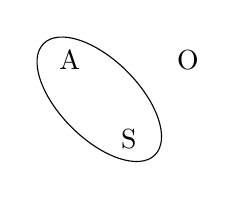
\begin{tikzpicture}
    \node[] at (0,1) {A};
    \node[] at (1.5,1) {O};
    \node[] at (0.75,0) {S};

    \draw[rotate around={45:(0.375,0.5)}] (0.375,0.5) ellipse (0.5 and 1);
  \end{tikzpicture}
  \caption{Nominative-accusative alignment}
  \label{fig:nom-acc-lang}
\end{figure}

In ergative-absolutive languages, the alignment is different. The subject of an intransitive verb (S) has the same marking as the object of the transitive verb (O), namely absolutive. The subject of the transitive verb (A) has its own marking, namely ergative. This is schematically shown in \ref{fig:erg-abs-lang}.

\begin{figure}[ht]
  \centering
  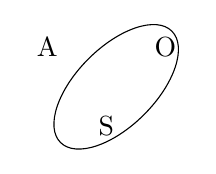
\begin{tikzpicture}
    \node[] at (0,1) {A};
    \node[] at (1.5,1) {O};
    \node[] at (0.75,0) {S};

    \draw[rotate around={135:(0.875,0.5)}] (0.875,0.5) ellipse (0.5 and 1);
  \end{tikzpicture}
  \caption{Ergative-absolutive alignment}
  \label{fig:erg-abs-lang}
\end{figure}

Note here that nominative-accusative languages use the same case marking for the same grammatical function (nominative for subject accusative for object), but ergative-absolutive languages do not.

\citet{bobaljik2006} describes how absolutives and ergatives behave with respect to whether they show agreement. There are languages in which there is agreement with both absolutives and ergatives. Besides that, there are languages in which there is only agreement with absolutives. Crucially, there is no language in which there is only agreement with ergatives. Absolutives are a heterogenous set with respect to grammatical function, i.e. they are subjects of intransitive verbs and objects of transitive verbs. However, with respect to showing agreement absolutives behave the same, and this behaviors is different from ergatives. This indicates that it is morphological case and not grammatical function that is the decisive factor.

\citeauthor{bobaljik2006} (following \citealt{marantz2000}) combines nominative-accusative and ergative-absolutive languages in the following way: accusative and ergative are dependent cases, and nominative or absolutive are unmarked case. Reformulating Figure \ref{fig:agr-sub-do-io} in terms of case instead of grammatical function gives the schema in Figure \ref{fig:agr-nom-acc-dat}.

\begin{figure}[H]
  \centering
  \begin{tikzpicture}
    \draw (0,1) circle (2.25);
    \draw [fill opacity=0.4, fill=LG] (0,0.5) circle (1.75);
    \draw [fill opacity=0.4, fill=DG] (0,0) circle (1.25);

    \node[] at (0,2.75) {unmarked case};
    \node[] at (0,1.5) {dependent case};
    \node[] at (0,0) {dative};

    \node[] at (2.5,3) {\footnotesize{● Japanese}};
    \node[] at (2.25,2) {\footnotesize{● German}};
    \node[] at (2,1) {\footnotesize{● Hungarian}};
    \node[] at (1.375,0) {\footnotesize{● Basque}};
  \end{tikzpicture}
  \caption{\posscitealt{bobaljik2006} actual schema}
  \label{fig:agr-def-dep-dat}
\end{figure}

This formulation in terms of case rather than grammatical function works as follows for the examples I gave earlier.
First, Japanese is a language that does not show any agreement, as shown in \ref{ex:japanese-agr}. There is no agreement with the unmarked case (here the nominative), not with the dependent case (here the accusative) and not with the dative case.
Second, German is a language that shows agreement only with the unmarked case, as shown in \ref{ex:german-agr}. The morpheme \tit{-st} on the predicate agrees with the element in unmarked nominative case \tit{du} `you'. There is no agreement with the dependent accusative case or with the dative case.
Third, Hungarian is a language that shows agreement with the unmarked and the dependent case, as shown in \ref{ex:hungarian-agr}. The portmanteau morpheme \tit{-om} on the predicates agrees with the element in unmarked nominative case \tit{én} `I' and the element in dependent accusative case \tit{a könyvet} `the book'.
Last, Basque is a language that shows agreement with the unmarked, the dependent and the dative case, as shown in \ref{ex:basque-agr}. The morpheme \tit{-zu} on the auxiliary agrees with the element in dependent ergative case \tit{zuk} `you'. The morpheme \tit{d-} on the auxiliary agrees with the element in unmarked absolutive case \tit{liburua} `the book'. The morpheme \tit{-ta} on the auxiliary agrees with the element in dative case \tit{niri} `me'.

In the languages I discuss in this dissertation, I focus on languages that have nominative as unmarked case and accusative as dependent case, so Figure \ref{fig:agr-nom-acc-dat} suffices.

\begin{figure}[ht]
  \centering
  \begin{tikzpicture}
    \draw (0,1) circle (2.25);
    \draw [fill opacity=0.4, fill=LG] (0,0.5) circle (1.75);
    \draw [fill opacity=0.4, fill=DG] (0,0) circle (1.25);

    \node[] at (0,2.75) {\ac{nom}};
    \node[] at (0,1.75) {\ac{acc}};
    \node[] at (0,0) {\ac{dat}};
  \end{tikzpicture}
  \label{fig:agr-nom-acc-dat}
  \caption{\posscitealt{bobaljik2006} simplified schema}
\end{figure}

In sum, this section has shown that agreement follows the same implicational hierarchy as the case scale in headless relatives: \ac{nom} < \ac{acc} < \ac{dat}.


\subsection{Relativization}

Relativization refers to the process in which a relative clause is derived from a non-relative clause. An example of the non-relative clause is given in \ref{ex:rel-non}. The relative clause derived from that is shown in \ref{ex:rel-realati}. The head of the relative clause is \tit{woman} and precedes the clause. The relative pronoun follows the head. The head of the head does not appear in the relative clause anymore.

\ex.
\a. You like the woman. \label{ex:rel-non}
\b. \tbf{the} \tbf{woman}, who you like \label{ex:rel-realati}

In \ref{ex:rel-realati}, it is the object of the clause that is relativized. It differs per language which elements can be relativized with a particular strategy. Just like the distribution was not random for agreement, it is not random which elements can be relativized. Instead, there is an implicational hierarchy that is identical to the one observed for the case scale: \ac{nom} < \ac{acc} < \ac{dat}.

\citet{keenan1977} formulated the implicational hierarchy in terms of the grammatical functions subject, direct object and indirect object.\footnote{
\citet{keenan1977} also included obliques, possessives and objects of comparison on the lowest end of the hierarchy. I leave them out here, because they are not relevant for the discussion.
}
The implicational hierarchy is schematically represented in Figure \ref{fig:rel-sub-do-io}. It should be read as follows: if a language allows a particular relativization strategy of the grammatical function in a particular circle, it also allows this relativization strategy of the grammatical function of the circle around it. The languages in the figure give examples of the circles they are in.

\begin{figure}[ht]
  \centering
  \begin{tikzpicture}
    \draw (0,1) circle (2.25);
    \draw [fill opacity=0.4, fill=LG] (0,0.5) circle (1.75);
    \draw [fill opacity=0.4, fill=DG] (0,0) circle (1.25);

    \node[] at (0,2.75) {subject};
    \node[] at (0,1.5) {direct object};
    \node[align=center] at (0,0) {indirect\\ object};

    \node[] at (2.25,2) {\footnotesize{● Malagasy/German}};
    \node[] at (2,1) {\footnotesize{● Malay}};
    \node[] at (1.375,0) {\footnotesize{● Basque}};
  \end{tikzpicture}
  \caption{Schema for relativization}
  \label{fig:rel-sub-do-io}
\end{figure}

There are four types of languages possible: first, a language that allows only the subject to be relativized with a particular strategy and not the direct and indirect object; second, a language that allows the subject and direct object to be relativized with a particular strategy but not the indirect object; and third, a language that allows the subject, the direct object and the indirect object to be relativized with a particular strategy.

Malagasy is an example of a language that allows subjects to be relativized using a particular strategy, but not direct and indirect objects. \ref{ex:malagasy-decl} is an example of a declarative sentence in Malagasy. It is a transitive sentence that contains the subject \tit{ny mpianatra} `the student' and the direct object \tit{ny vehivavy} `the woman'.

\exg. Nahita ny vehivavy ny mpianatra.\\
 saw the woman the student\\
 `The student saw the woman.' \flushfill{Malagasy, \pgcitealt{keenan1977}{70}}\label{ex:malagasy-decl}

In \ref{ex:malagasy-subj}, the subject from the declarative sentence, marked in bold, is relativized. The subject \tit{ny mpianatra} `the student' appears in the first position of the clause. It is followed by the invariable relativizer \tit{izay} `that'. After that, the rest of the relative clause follows, in this case \tit{nahita ny vehivavy} `saw the woman'.

\exg. \tbf{ny} \tbf{mpianatra} izay nahita ny vehivavy\\
 the student that saw the woman\\
 `the student that saw the woman' \flushfill{Malagasy, \pgcitealt{keenan1977}{70}, my boldfacing}\label{ex:malagasy-subj}

The object of \ref{ex:malagasy-decl} cannot be relativized in the same way, as shown in \ref{ex:malagasy-no-do}. Here the object \tit{ny vehivavy} `the woman', marked in bold, appears in the first position of the clause. It is again followed by the relativizer \tit{izay} `that' and the rest of the relative clause, which is here \tit{nahita ny mpianatra} `saw the student'. This example is ungrammatical.

\exg. *\tbf{ny} \tbf{vehivavy} izay nahita ny mpianatra\\
 the woman that saw the student\\
 `the woman that the student saw' \flushfill{Malagasy, \pgcitealt{keenan1977}{70}, my boldfacing}\label{ex:malagasy-no-do}

Later in this section I draw the parallel between subject and nominative, direct object and accusative and indirect object and dative \citep[after][]{caha2009}. As Malagasy does not have any overt morphological system, it does not hold that the subject corresponds to the nominative in this case.
German is another example of a language that allows subjects to be relativized using a particular strategy, but not direct and indirect object. This strategy is the participle construction \citep{keenan1977}. This strategy is a secondary strategy that exist besides the main strategy that can be used to relativize direct and indirect objects. \ref{ex:german-rel-decl} is an example of a declarative sentence in German. It is a transitive sentence that contains the subject \tit{die Frau} `the woman' and the object \tit{der Mann} `the man'.

\exg. Die Frau küsst den Mann.\\
the woman kisses the man\\
`The woman is kissing the man.' \flushfill{German}\label{ex:german-rel-decl}

The subject from the declarative in \ref{ex:german-rel-decl}, sentence \tit{die Frau} `the woman', is relativized in \ref{ex:german-rel-subj}. The predicate from the declarative clause \tit{küsst} `kisses' is turned in into the participle \tit{küssende} `kissing'. The participle appears at the end of the reduced relative clause \tit{den Mann küssende} `the man kissing'. The reduced relative clause directly precedes the noun of the subject, creating distance between the determiner \tit{die} `the' and \tit{Frau} `woman', which are both marked in bold.

\exg. \tbf{die} den Mann küssende \tbf{Frau}\\
 the the man kissing woman\\
 `the woman who is kissing the man' \flushfill{German}\label{ex:german-rel-subj}

The object from the declarative sentence in \ref{ex:german-rel-decl}, \tit{den Mann} `the man', cannot be relativized like the subject, as shown in \ref{ex:german-rel-no-do}. Again, the predicate from the declarative clause \tit{küsst} `kisses' is turned in into the participle \tit{küssende} `kissing'. The participle appears at the end of the relative clause \tit{die Frau küssende} `the woman kissing'. The reduced relative clause directly precedes the noun of the object, creating distance between the determiner \tit{der} `the' and \tit{Mann} `man', which are both marked in bold. This example is ungrammatical.

\exg. *\tbf{den} die Frau küssende \tbf{Mann}\\
 the the woman kissing man\\
 intended: `the man that the woman is kissing' \flushfill{German}\label{ex:german-rel-no-do}

Malay is an example of a language that has a relativization strategy for subjects and direct objects, but not for indirect objects. \ref{ex:malay-do} shows an example in which the object is relativized. The object here is \tit{ayam} `chicken', marked in bold. It is followed by the relativizer \tit{yang} `that'. After that, the rest of the relative clause \tit{Aminah sedang memakan} `Aminah is eating' follows. The same strategy works to relativize subjects, which is not illustrated with an example.

\exg. Ali bunoh \tbf{ayam} yang Aminah sedang memakan.\\
 Ali kill chicken that Aminah \ac{prog} eat\\
 `Ali killed the chicken that Aminah is eating.' \flushfill{Malay, \pgcitealt{keenan1977}{71}, my boldfacing}\label{ex:malay-do}

Indirect objects cannot be relativized using the same strategy. \ref{ex:malay-decl} is an example of a ditransitive sentence in Malay. The indirect object \tit{kapada perempuan itu} `to the woman' cannot be relativized using \tit{yang}.

\exg. Ali beri {ubi kentang} itu kapada perempuan itu.\\
 Ali give potato the to woman the\\
 `Ali gave the potato to the woman.'\label{ex:malay-decl} \flushfill{Malay, \pgcitealt{keenan1977}{71}}

This is illustrated by the examples in \ref{ex:malay-no-io}. In \ref{ex:malay-no-io1}, the direct object \tit{perempuan kapada} `to the woman', marked in bold, appears in the first position of the clause. It is followed by the relativizer \tit{yang} `that' and the rest of the relative clause \tit{Ali beri ubi kentang itu kapada} `Ali gave the potato to'. This example in ungrammatical.
The example in \ref{ex:malay-no-io2} differs from \ref{ex:malay-no-io1} in that the preposition \tit{kapada} `to' has been moved such that it precedes the relativizer \tit{yang} `that'. This example is ungrammatical as well, indicating this was not the reason for the ungrammaticality.

\ex.\label{ex:malay-no-io}
\ag. *\tbf{perempuan} yang Ali beri {ubi kentang} itu kapada\\
 woman that Ali give potato the to\\\label{ex:malay-no-io1}
\bg. *\tbf{perempuan} \tbf{kapada} yang Ali beri {ubi kentang} itu\\
 woman to who Ali give potato that\\\flushfill{Malay, \pgcitealt{keenan1977}{71}, my boldfacing}\label{ex:malay-no-io2}

% Later in this section I draw the parallel between subject and nominative, direct object and accusative and indirect object and dative \citep[after][]{caha2009}. As Malagasy does not have any overt morphological system, it does not hold that the subject corresponds to the nominative in this case.
% Finnish is another example..
%
%  (12) a. Poydalla tanssinut poika oli sairas.
%  on-table having-danced boy was sick
%  'The boy who had danced on the table was sick.'
%  b. Nakemani poika tanssi poydalla.
%  I-having-seen boy danced on-table
%  'The boy that I saw danced on the table.'



Basque is an example of a language that has a particular relativization strategy for subjects, direct objects and indirect objects. \ref{ex:basque-decl} is an example of a declarative ditransitive sentence in Basque. The sentence contains the subject \tit{gizonak} `the man', the direct object \tit{liburua} `the book' and the indirect object \tit{emakumeari} `the woman'.

\exg. Gizon-a-k emakume-a-ri liburu-a eman dio.\\
 man-\ac{def}-\ac{erg} woman-\ac{def}-\ac{dat} book-\ac{def}.\ac{abs} give has\\
 `The man has given the book to the woman.' \flushfill{Basque, \pgcitealt{keenan1977}{72}}\label{ex:basque-decl}

A relative clause in Basque appears in the prenominal position and it is marked by the invariable marker \tit{-n}.\footnote{
Additionally, the relativized positions do not appear in verbal agreement anymore, but this not visible in the example, because they are all phonologically zero.
}
\ref{ex:basque-sub} shows the three relativizations that are derived from \ref{ex:basque-decl}.
In \ref{ex:basque-sub}, the ergative subject \tit{gizonak} `the man' from \ref{ex:basque-decl} is relativized. The head \tit{gizona} `the man', marked in bold, has lost its ergative marker \tit{-k}, and follows the relative clause \tit{makumeari liburua eman dio} `who has given the book to the woman'. The suffix \tit{-n} is attached to the relative clause.
In \ref{ex:basque-do}, the absolutive direct object \tit{liburua} `the book' from \ref{ex:basque-decl} is relativized. The head \tit{liburua} `the book', marked in bold, follows the relative clause \tit{gizonak emakumeari eman dion} `that the man has given to the woman'.\footnote{
The absolutive direct object \tit{liburua} `the book' does not have an additional overt absolutive marker, so this difference cannot be observed when it is relativized.
}
The suffix \tit{-n} is attached to the relative clause.
In \ref{ex:basque-io}, the dative indirect object \tit{emakumeari} `the woman' from \ref{ex:basque-decl} is relativized. The head \tit{emakumea} `the man', marked in bold, has lost its dative marker \tit{-ri}, and follows the relative clause \tit{gizonak liburua eman dion} `that the man has given the book to'. The suffix \tit{-n} is attached to the relative clause.

\ex.\label{ex:basque-rel}
\ag. emakume-a-ri liburu-a eman dio-n \tbf{gizon-a}\\
 woman-\ac{def}-\ac{dat} book-\ac{def}.\ac{abs} give has-\ac{rel} man-\ac{def}\\
 `the man who has given the book to the woman'\label{ex:basque-sub}
\bg. gizon-a-k emakume-a-ri eman dio-n \tbf{liburu-a}\\
 man-\ac{def}-\ac{erg} woman-\ac{def}-\ac{dat} give has-\ac{rel} book-\ac{def}\\
 `the book that the man has given to the woman'\label{ex:basque-do}
\bg. gizon-a-k liburu-a eman dio-n \tbf{emakume-a}\\
 man-\ac{def}-\ac{erg} book-\ac{def}.\ac{abs} give has-\ac{rel} woman-\ac{def}\\
 `the woman that the man has given the book to' \flushfill{Basque, \pgcitealt{keenan1977}{72}, my boldfacing}\label{ex:basque-io}

\citet{caha2009} argues that the implicational hierarchy is more accurate if it is stated in terms of case rather than grammatical function. The main argument comes from ergative-absolutive languages, which was also one of \posscitet{bobaljik2006} argument with the implicational hierarchy for agreement. \citet{keenan1977} point out that some ergative-absolutive languages form a counterexample to their hierarchy. \citet{caha2009} points out that ergative subjects and oblique noun phrases use the same relativization strategy, which is not allowed with absolutive objects (which is also briefly mentioned in
\citealt{bobaljik2006}).

Reformulating Figure \ref{fig:agr-sub-do-io} in terms of case instead of grammatical function gives the schema in Figure \ref{fig:agr-nom-acc-dat}.

\begin{figure}[ht]
  \centering
  \begin{tikzpicture}
    \draw (0,1) circle (2.25);
    \draw [fill opacity=0.4, fill=LG] (0,0.5) circle (1.75);
    \draw [fill opacity=0.4, fill=DG] (0,0) circle (1.25);

    \node[] at (0,2.75) {unmarked case};
    \node[] at (0,1.5) {dependent case};
    \node[align=center] at (0,0) {dative};

    \node[] at (2.25,2) {\footnotesize{● Malagasy/German}};
    \node[] at (2,1) {\footnotesize{● Malay}};
    \node[] at (1.375,0) {\footnotesize{● Basque}};
  \end{tikzpicture}
  \caption{Schema for relativization}
  \label{fig:rel-def-dep-dat}
\end{figure}

This formulation in terms of case rather than grammatical function works as follows for the examples I gave earlier.

First, German is a language that has a particular relativization strategy for the unmarked case, as shown in \ref{ex:german-rel-subj}. The unmarked nominative case can be relativized with a reduced relative clause, but the dependent accusative case and the dative case cannot.
Second,
Last, Basque is a language that has a particular relativization strategy for unmarked, dependent and dative case, as shown in \ref{ex:basque-rel}. The unmarked ergative, dependent absolutive and dative case can be relativized by extraposing the head, and marking it with the invariable marker \tit{-n}.

In the languages I discuss in this dissertation, I focus on languages that have nominative as unmarked case and accusative as dependent case, so Figure \ref{fig:rel-nom-acc-dat} suffices.

\begin{figure}[ht]
  \centering
  \begin{tikzpicture}
    \draw (0,1) circle (2.25);
    \draw [fill opacity=0.4, fill=LG] (0,0.5) circle (1.75);
    \draw [fill opacity=0.4, fill=DG] (0,0) circle (1.25);

    \node[] at (0,2.75) {nominative};
    \node[] at (0,1.5) {accusative};
    \node[align=center] at (0,0) {dative};
  \end{tikzpicture}
  \caption{Schema for relativization}
  \label{fig:rel-nom-acc-dat}
\end{figure}

In sum, this section has shown that relativization follows the same implicational hierarchy as agreement and as the case scale in headless relatives: \ac{nom} < \ac{acc} < \ac{dat}.


\section{In morphology}\label{sec:case-morphology}

In the two previous sections I showed that the case scale \ac{nom} < \ac{acc} < \ac{dat} can be observed in three syntactic phenomena. First, it shows up in case competition in headless relatives. Second, the case scale forms the basis for the implicational hierarchy observed in agreement across languages. Third, the identical implicational holds for relativization strategies cross-linguistically.

In this section, I show that this same case scale also shows up in morphology. First, syncretism only targets continuous regions on the case scale. Second, several languages show formal containment that mirrors the case scale.


\subsection{Syncretism}

Syncretism refers to the phenomenon whereby two or more different functions are fulfilled by a single form \citep[cf.][]{baerman2002}. In this section I discuss literature that shows that syncretism patterns among nominative, accusative and dative are not random. Instead, they pattern along the case scale \ac{nom} < \ac{acc} < \ac{dat}.

It has widely been observed that syncretism is restricted by the linear sequence \ac{nom} --- \ac{acc} --- \ac{dat} \citep{baerman2005,caha2009,zompi2017} (and see \citealt{mcfadden2018,smith2019} for similar claims concerning root suppletion). That is, if one orders cases in this linear sequence, only contiguous regions in the sequence turn out to be syncretic.
Following that, four possible patterns are attested crosslinguistically. First, all three cases are syncretic. Second, nominative and accusative are syncretic and the dative is not. Third, the accusative and the dative are syncretic and the nominative is not. Fourth, all cases are non-syncretic.

There is one pattern that is not attested crosslinguistically. This pattern does not target continuous regions, but non-contiguous ones: nominative and dative are syncretic and accusative is not. In other words, there is no ABA pattern (in which a form B intervenes between the two identically formed As) \citep{bobaljik2012}.

Table \ref{tbl:syncretisms} shows examples for each of these possible patterns.
I give an example from three distinct forms from Faroese. The second person singular is \tit{tú} `you' for nominative, \tit{teg} `you' for accusative and \tit{tær} `you' for dative \pgcitep{lockwood1977}{70}.
I give an example from a syncretism between nominative, accusative and dative from Dutch. The second person plural pronoun is \tit{jullie} `you.\ac{pl}' is syncretic between nominative, accusative and dative.
I give an example from a syncretism between accusative and dative but not nominative from Icelandic. The first person singular plural is \tit{okkur} `us' is syncretic between accusative and dative. The nominative has a separate form: \tit{við} `we' \pgcitep{einarsson1949}{68}.
I give an example from a syncretism between nominative and accusative but not dative from German. The third person singular feminine \tit{sie} `she/her' is syncretic between nominative and accusative. The dative has a separate form: \tit{ihr} `her'.
Crucially, to the best of my knowledge, there is no language in which the nominative and the dative are syncretic but the accusative is not.

\begin{table}[ht]
  \center
  \caption {}
    % !TEX root = ../thesis.tex

\begin{tabular}{cccccccc}
  \toprule
      \multicolumn{3}{c}{pattern}
        & \ac{nom}
        & \ac{acc}
        & \ac{dat}
        & translation
        & language \\
  \cmidrule(lr){1-3} \cmidrule(lr){4-6} \cmidrule(lr){7-7} \cmidrule(lr){8-8}
      A & A & A
        & \cellcolor{LG}jullie
        & \cellcolor{LG}jullie
        & \cellcolor{LG}jullie
        & 2\ac{pl}
        & Dutch \\
      A & A & B
        & \cellcolor{LG}sie
        & \cellcolor{LG}sie
        & ihr
        & 3\ac{sg}.\ac{f}
        & German \\
      A & B & B
        & við
        & \cellcolor{LG}okkur
        & \cellcolor{LG}okkur
        & 1\ac{pl}
        & Icelandic \\
      A & B & C
        & tú
        & teg
        & tær
        & 2\ac{sg}
        & Faroese \\
      A & B & A
        & \cellcolor{LG}
        &
        & \cellcolor{LG}
        &
        & not attested \\
  \bottomrule
\end{tabular}

  \label{tbl:syncretisms}
\end{table}

In sum, case syncretism follows the ordering of the case scale in headless relatives: \ac{nom} < \ac{acc} < \ac{dat}.


\subsection{Formal containment}

This section shows a second way in which \ac{nom} < \ac{acc} < \ac{dat} is reflected in morphology: formal containment \citep[cf.][]{smith2019,zompi2017,caha2010}. In some languages, the form that is used for the accusative literally contains the form that is used for the nominative. In turn, the forms for the dative contains the form for the accusative. I illustrate this phenomenon with examples from Khanty.

Khanty (or Ostyak) shows formal containment in some of its pronouns (\pgcitealt{nikolaeva1999}{16} after \citealt{smith2019}). Three examples are given in Table \ref{tbl:cont-khanty}.

The nominative form for the first person singular is \tit{ma} `I.\ac{nom}'. The form for the accusative is \tit{ma:ne:m} `me'. This is the form for the nominative \tit{ma} plus the accusative marker \tit{-ne:m}. The form for the dative is \tit{ma:ne:mna} `me'. This is the form for the accusative \tit{ma:ne:m} plus the dative marker \tit{-na}. So, dative formally contains the accusative, and the accusative formally contains the nominative.

The third person singular and first person plural show the same pattern. The accusative forms \tit{luwe:l} `him/her' and \tit{muŋe:w} `us' contain the nominative forms \tit{luw} and the \tit{muŋ} plus the accusative marker \tit{-e:l} or \tit{-e:w}. The dative forms \tit{luwe:lna} `him/her' and \tit{muŋe:wna} `us' contain the accusative forms \tit{luwe:l} and \tit{muŋe:w} plus the dative marker \tit{-na}. Again, the dative formally contains the accusative, which in turn contains the nominative.

\begin{table}[ht]
  \center
  \caption {Case containment in Khanty}
  \begin{tabular}{clll}
  \toprule
            & \ac{1}\ac{sg}
            & \ac{3}\ac{sg}
            & \ac{1}\ac{pl}                           \\
            \cmidrule{2-4}
  \ac{nom}  & ma
            & luw
            & muŋ                                     \\
  \ac{acc}  & ma:\tbf{-ne:m}
            & luw\tbf{-e:l}
            & muŋ\tbf{-e:w}                           \\
  \ac{dat}  & ma:\tbf{-ne:m}\tcol{DG}{\tbf{-na}}
            & luw\tbf{-e:l}\tcol{DG}{\tbf{-na}}
            & muŋ\tbf{-e:w}\tcol{DG}{\tbf{-na}}       \\
  \bottomrule
  \end{tabular}
  \label{tbl:cont-khanty}
\end{table}

Other languages that show this phenomenon are West Tocharian \citep{gippert1987} and Vlakh and Kalderaš Romani (respectively \citealt{friedman1991} and \citealt{boretzky1994}).

In sum, some languages morphologically look like \ac{nom}-\ac{acc}-\ac{dat}. This exactly reflects the case scale \ac{nom} < \ac{acc} < \ac{dat}.

\section{Summary}

Case competition in headless relatives adheres to the case scale in \ref{ex:case-scale-sum}. If the internal and external case differ, cases more on the right of the scale win over cases more to the left on the case.

\ex. \ac{nom} < \ac{acc} < \ac{dat}\label{ex:case-scale-sum}

This case scale is not only found in case competition in headless relatives. Implicational hierarchies regarding two syntactic phenomena appear across languages. The first one concerns agreement. If a language shows agreement with datives, it also shows agreement with accusatives and nominatives. If a language shows agreement with accusatives, it also shows agreement with nominatives.
The second implicational hierarchy concerns relativization. If a dative in a language can be relativized with a particular strategy, an accusative and a nominative can be too using the same strategy. If an accusative can be relativized with a particular strategy, so can a nominative with this strategy.

The case scale also shows up in morphological patterns. First, if the cases are ordered according to the case scale, syncretism only target continuous forms, no ABA pattern appears. Second, some languages show how the dative formally contains accusative, and how the accusative formally contains the nominative.

These phenomena show that the pattern observed in headless relatives is not something that stands on itself. The scale is a pattern that recurs across languages and across different phenomena. Therefore, it should not be treated as an special process with its own stipulated rule. Instead, it is something general that should also follow from general processes in languages.

The next chapter shows how features of the nominative, accusative and dative are organized. All facts presented in this chapter can be derived from the organization of these features.

% !TEX root = thesis.tex

\chapter{Case decomposition}\label{ch:decomposition}

This chapter provides a theory that derives the first aspect of case competition in headless relatives that I discuss in this dissertation.
This theory seeks to capture that headless relatives crosslinguistically adhere to the case scale \tsc{nom} < \tsc{acc} < \tsc{dat}.

In most existing accounts for case competition in headless relatives (\citealt[cf.][]{pittner1995,vogel2001,grosu2003,harbert1978}, an exception to this is \citealt{himmelreich2017}) the case scale is stipulated. Headless relatives are said to simply obey to that scale. \pgcitet{pittner1995}{fn.4} makes this explicit: ``One of the reviewers notes that an explanation in terms of a Case hierarchy is rather stipulative. However, as far as I know, nobody has suggested a nonstipulative explanation for these facts.''

In the previous chapter I showed that the case scale \ac{nom} < \ac{acc} < \ac{dat} is not specific to headless relatives, but it is a wide-spread phenomenon: it can also be observed in morphology (and in syntax).

Within morphology it appears in syncretism patterns and morphological case containment. \pgcitet{pittner1995}{201:fn.4} makes this link to morphology as well: ``Furthermore, the Case hierarchies receive some independent support by morphology as shown by the various inflectional paradigms.''

As I already eluded to in the summary of Chapter \ref{ch:introduction}, I am not after a theory in which the case scale is something construction-specific, or one in which syntax and morphology both have their own case scale. Instead, argue that there is a single trigger that is responsible for the case scales in different subparts of language (which is identical to what \citealt{caha2019} suggests for case competition in numeral phrases). Specifically, I show that the observed case scale naturally follows on the assumption that the case scale is deeply anchored in syntax. The case scales in morphology and syntax are merely reflexes of how case is organized in the linguistic system.\footnote{
\citet{himmelreich2017} works this intuition out in a different way.
}

This chapter is structured as follows. First, I introduce a specific cumulative case decomposition \citep{caha2009}. In the two following sections, I show how this case decomposition is able to derive the syncretism and morphological case containment facts from Chapter \ref{ch:recurring}. I make this concrete in the framework Nanosyntax \citep{starke2009}. Finally, I show how the case decomposition relates to the winner in case competition in headless relatives.


\section{The basic idea}

\citet{caha2009,caha2013} (followed by \citealt[cf.][]{starke2009,bobaljik2012,mcfadden2018,smith2019,vanbaal2018}) has extensively argued that case should be decomposed into privative features. Specifically, the decomposition is cumulative: each case has a different number of case features, and the number grows one by one.
This is illustrated in Table \ref{tbl:case-decomposed}. Accusative has all the features that nominative has (here \tsc{k}1) plus one extra (here \tsc{k}2). Dative has all the features accusative has (\tsc{k}1 and \tsc{k}2) plus one extra (\tsc{k}3).

\begin{table}[ht]
  \center
	\caption {Cumulative case decomposition}
		\begin{tabular}{ll}
    \toprule
    case      & features                  \\
    \midrule
    \ac{nom} & \tsc{k}1                    \\
    \ac{acc} & \tsc{k}1, \tsc{k}2           \\
    \ac{dat} & \tsc{k}1, \tsc{k}2, \tsc{k}3  \\
    \bottomrule
    \end{tabular}
    \label{tbl:case-decomposed}
\end{table}

Consider the case scale, repeated in repeated in \ref{ex:case-scale-derive}.

\ex. \ac{nom} < \ac{acc} < \ac{dat}\label{ex:case-scale-derive}

This scale actually indicates containment.
Nominative corresponds to a set of features (\tsc{k}1) that is contained in the set of features of accusative (\tsc{k}1 and \tsc{k}2).
Similarly, nominative corresponds to a set of features that is contained in the set of features of dative (\tsc{k}1, \tsc{k}2 and \tsc{k}3).
Lastly, accusative corresponds to a set of features (\tsc{k}1 and \tsc{k}2) that is contained in the set of features of dative (\tsc{k}1, \tsc{k}2 and \tsc{k}3).

The decomposition in Table \ref{tbl:case-decomposed} forms the basis to derive the case scale effects observed in Chapter \ref{ch:recurring}. The following sections show how morphological case containment and syncretism effects follow naturally. After that, I show how the decomposition also derives the case competition facts in headless relatives.


\section{Deriving syncretism}\label{sec:syncretism}

Case syncretism follows the ordering of the case scale. Along this scale, only contiguous regions in the sequence are syncretic. In this section I show how case syncretism patterns can be derived from the case decomposition shown in Table \ref{tbl:case-decomposed}.
In Table \ref{tbl:syncretisms-derive} I repeat the examples that shows the possible and impossible syncretism patterns.

\begin{table}[ht]
  \center
  \caption {Syncretism patterns in Germanic pronouns (repeated)}
    % !TEX root = ../thesis.tex

\begin{tabular}{cccccccc}
  \toprule
      \multicolumn{3}{c}{pattern}
        & \ac{nom}
        & \ac{acc}
        & \ac{dat}
        & translation
        & language \\
  \cmidrule(lr){1-3} \cmidrule(lr){4-6} \cmidrule(lr){7-7} \cmidrule(lr){8-8}
      A & A & A
        & \cellcolor{LG}jullie
        & \cellcolor{LG}jullie
        & \cellcolor{LG}jullie
        & 2\ac{pl}
        & Dutch \\
      A & A & B
        & \cellcolor{LG}sie
        & \cellcolor{LG}sie
        & ihr
        & 3\ac{sg}.\ac{f}
        & German \\
      A & B & B
        & við
        & \cellcolor{LG}okkur
        & \cellcolor{LG}okkur
        & 1\ac{pl}
        & Icelandic \\
      A & B & C
        & tú
        & teg
        & tær
        & 2\ac{sg}
        & Faroese \\
      A & B & A
        & \cellcolor{LG}
        &
        & \cellcolor{LG}
        &
        & not attested \\
  \bottomrule
\end{tabular}

  \label{tbl:syncretisms-derive}
\end{table}

Table \ref{tbl:syncretisms-derive} shows that if one orders cases in the linear sequence \ac{nom} --- \ac{acc} --- \ac{dat}, only contiguous regions in the sequence turn out to be syncretic. First, all three cases can be non-syncretic, as in Faroese. Second, all three cases can be syncretic, as in Dutch. Third, the accusative and the dative can be syncretic and the nominative not, as in Icelandic. Fourth, nominative and accusative can be syncretic and the dative not, as in German. The pattern that is not attested crosslinguistically is the one that targets non-contiguous regions in the table, the ABA pattern \citep{baerman2005,caha2009,zompi2017}.

The syncretism facts follow in a system in which the case is decomposed as in Table \ref{tbl:case-decomposed} and in which lexicalization relies on containment. The latter means that a phonological form is not only inserted when the lexical specification is identical to the syntax, but also when the syntactic features are a subset of the lexical specification. The intuition is the following. Syncretic forms are realized by a single `lexical entry' from the `lexicon'. I elaborate on the terms lexical entry and lexicon shortly.
A lexical entry can be applied if it contains all features, as long as there is no more specific one. This system can generate the patterns ABC, AAA, ABB and AAB, but not ABA.

Before I show how the four attested patterns can be derived (and the unattested one cannot), I need to make some theoretical assumptions explicit about Nanosyntax, the framework in which this dissertation is worked out. First, I show how the Nanosyntactic system is set up in such a way that morphological patterns (like syncretism, but also morphological containment) can inform us about the way syntax is structured. Therefore, I briefly discuss the general architecture of Nanosyntax, its postsyntactic lexicon, and the content and shape of lexical entries. Lastly, I discuss how multiple features (like \tsc{k}1, \tsc{k}2 and \tsc{k}3 from Table \ref{tbl:case-decomposed}) can be spelled out by a single phonological element using phrasal spellout.

In Nanosyntax, syntax starts with atomic features, and it builds complex syntactic trees. Specifically, there are no `feature bundles' (from a pre-syntactic lexicon) that enter the syntax. The only way complex feature structures come to exist is a a result of merge.
After syntax (actually, each instance of merge), the syntactic structure is matched against the lexicon for pronunciation. The lexicon `translates' between lexical trees (i.e. syntactic representations) on the one hand and phonology (PF) and concepts (CF) on the other hand.\footnote{
Throughout the dissertation I call the syntactic representations in the lexicon `lexical trees' in order to distinguish them from syntactic structures in the syntax.
}

In Nanosyntax, the lexicon contains lexical entries, which are links between lexical trees, phonological representations and conceptual representations \citep{starke2014}.\footnote{
The lexical tree does not have to correspond to both a phonological and a conceptual representation. Lexical trees that only correspond to a conceptual representations and not to phonological representations are (phrasal or clausal) idioms. Lexical trees that only correspond to phonological representations but not to conceptual representations are for instance irregular plurals.
} I leave the conceptual representation out of discussion for now, as it is not relevant for the discussion here. The fact that only syntax can create complex feature structures also has a consequence for lexical entries in the lexicon.
Syntactic structures are constrained by certain principles, such that only well-formed syntactic structures exist. Since lexical entries in the lexicon link lexical trees to phonological and conceptual representation, these lexical trees are constrained by the same principles as syntactic structures are.
As a result, the lexicon only contains well-formed lexical trees. The lexicon does not contain unstructured `feature bundles', because they could never be created by syntax.

Following this logic, a feature bundle as in \ref{ex:feature-set} cannot exist. It cannot have entered syntax, because syntax starts with atomic features. It can also not be created by syntax, because complex structures can only be created with merge.

\ex. [ \tsc{k}1, \tsc{k}2, \tsc{k}3 ]\label{ex:feature-set}

Instead, a possible lexical tree looks as in \ref{ex:feature-structure}. The features are merged one by one in a binary structure.

\ex. \begin{forest} boom
  [\ac{dat}P
      [\tsc{k}3]
      [\ac{acc}P
          [\tsc{k}2]
          [\tsc{k}1]
      ]
  ]
\end{forest}\label{ex:feature-structure}

This structure leads to the concept of phrasal spellout: not terminals but multiple syntactic heads (phrases) are realized with a single piece of phonology (i.e. a single morpheme). Applying this to \ref{ex:feature-structure}, not the terminals \tsc{k}1, \tsc{k}2 and \tsc{k}3 receive a realization, but \ac{acc}P and \ac{dat}P are spelled out. A necessary requirement is that these multiple syntactic heads form a constituent. That means that \ac{dat}P cannot be spelled out without \ac{acc}P.

Let me illustrate all of the above with the Faroese pronouns from Table \ref{tbl:syncretisms-derive}. I simplify the situation in two respects. First, I do not show the internal complexity of the pronouns, including person and number features. Instead, I give a triangle, indicating that this is a complex syntactic structure. I refer to is as the person-number phrase it refers to, e.g. 2\ac{sg}P. Second, in this simplified representation I consider the Faroese pronouns to be monomorphemic. I ignore the fact that all three pronouns have the stem \tit{t} with a suffix following it.

The lexical entry for \tit{tú} is given in \ref{ex:faroese-tu-lexicon}. The lexical tree consists of the second person singular pronoun (the 2\ac{sg}P), and \tsc{k}1, making it a \ac{nom}P. The phonological representation that is linked to the lexical tree is \tit{tú}.\footnote{
Throughout the dissertation, I use lexical trees and phonological forms connected by a double arrow (⇔) to refer to a lexical entry.
}

\ex.
\begin{forest} boom
  [\ac{nom}P
      [\tsc{k}1]
      [2\ac{sg}P
          [\phantom{xxx}, roof]
      ]
  ]
  {\draw (.east) node[right]{⇔ \tit{tú}}; }
\end{forest}
\label{ex:faroese-tu-lexicon}

The lexical entry for \tit{teg} is given in \ref{ex:faroese-teg-lexicon}. The lexical tree consists of all the features of the lexical tree in \ref{ex:faroese-tu-lexicon}, plus \tsc{k}2, making it an \ac{acc}P. The linked phonological representation is \tit{teg}.

\ex.
\begin{forest} boom
  [\ac{acc}P
      [\tsc{k}2]
      [\ac{nom}P
          [\tsc{k}1]
          [2\ac{sg}P
              [\phantom{xxx}, roof]
          ]
      ]
  ]
  {\draw (.east) node[right]{⇔ \tit{teg}}; }
\end{forest}
\label{ex:faroese-teg-lexicon}

The lexical entry for \tit{tær} is given in \ref{ex:faroese-taer-lexicon}. The lexical tree consists of all the features of the lexical tree in \ref{ex:faroese-teg-lexicon}, plus \tsc{k}3, making it an \ac{dat}P. The linked phonological representation is \tit{tær}.

\ex.
\begin{forest} boom
  [\ac{dat}P
      [\tsc{k}3]
      [\ac{acc}P
          [\tsc{k}2]
          [\ac{nom}P
              [\tsc{k}1]
              [2\ac{sg}P
                  [\phantom{xxx}, roof]
              ]
          ]
      ]
  ]
  {\draw (.east) node[right]{⇔ \tit{tær}}; }
\end{forest}
\label{ex:faroese-taer-lexicon}

The lexical trees and their phonological counterparts I gave in \ref{ex:faroese-tu-lexicon} to \ref{ex:faroese-taer-lexicon} are lexical entries.
These lexical entries are used to spell out syntactic structures. I give examples of syntactic structures in \ref{ex:faroese-tu-spellout} to \ref{ex:faroese-taer-spellout}.

The lexical tree in \ref{ex:faroese-tu-lexicon} is identical to the syntactic structure in \ref{ex:faroese-tu-spellout}. Therefore, this syntactic structure is spelled out as \tit{tú}.\footnote{
Throughout this dissertation I circle the part of the syntactic structure that corresponds to a particular lexical entry, and I place the corresponding phonology under it.
}

\ex. \begin{forest} boom
[\ac{nom}P,
tikz={
\node[label=below:\tit{tú},
draw,circle,
scale=0.8,
fit to=tree]{};
}
    [\tsc{k}1]
    [2\ac{sg}P
        [\phantom{xxx}, roof]
    ]
]
\end{forest}
\label{ex:faroese-tu-spellout}

The lexical tree in \ref{ex:faroese-teg-lexicon} is identical to the syntactic structure in \ref{ex:faroese-teg-spellout}, and it is spelled out as \tit{teg}.

\ex. \begin{forest} boom
[\ac{acc}P,
tikz={
\node[label=below:\tit{teg},
draw,circle,
scale=0.825,
fit to=tree]{};
}
    [\tsc{k}2]
    [\ac{nom}P
        [\tsc{k}1]
        [2\ac{sg}P
            [\phantom{xxx}, roof]
        ]
    ]
]
\end{forest}
\label{ex:faroese-teg-spellout}

The lexical tree in \ref{ex:faroese-taer-lexicon} is identical to the syntactic structure in \ref{ex:faroese-taer-spellout}, and it is spelled out as \tit{tær}.

\ex. \begin{forest} boom
[\ac{dat}P,
tikz={
\node[label=below:\tit{tær},
draw,circle,
scale=0.85,
fit to=tree]{};
}
    [\tsc{k}3]
    [\ac{acc}P
        [\tsc{k}2]
        [\ac{nom}P
            [\tsc{k}1]
            [2\ac{sg}P
                [\phantom{xxx}, roof]
            ]
        ]
    ]
]
\end{forest}
\label{ex:faroese-taer-spellout}

In the Faroese examples above, the syntactic structures are all identical to the lexical trees. However, Nanosyntax assumes that to be a successful match, identity is not a necessary requirement. Instead, matching relies on a containment relation. This is formalized as in \ref{ex:superset-principle}.

\ex. \tbf{The Superset Principle} \citet{starke2009}:\\
A lexically stored tree matches a syntactic node iff the lexically stored tree contains the syntactic node.
\label{ex:superset-principle}

Let me illustrate this with the Dutch second person plural pronoun from Table \ref{tbl:syncretisms-derive}. This pronoun is syncretic between between the nominative, accusative and dative.
The lexicon only contains a single lexical entry, namely \ref{ex:dutch-jullie-lexicon}. The lexical tree consists of the complex lexical tree that corresponds to the second person plural pronoun (the \ac{2}\ac{pl}P), and \tsc{k}1, \tsc{k}2 and \tsc{k}3 making it a \ac{dat}P. The phonological representation that is linked to the lexical tree is \tit{jullie}.
The nominative, the accusative and the dative can all be spelled out with this single lexical entry using the Superset Principle in \ref{ex:superset-principle}.

\ex.
\begin{forest} boom
  [\ac{dat}P
      [\tsc{k}3]
      [\ac{acc}P
          [\tsc{k}2]
          [\ac{nom}P
              [\tsc{k}1]
              [2\ac{pl}P
                  [\phantom{xxx}, roof]
              ]
          ]
      ]
  ]
  {\draw (.east) node[right]{⇔ \tit{jullie}}; }
\end{forest}
\label{ex:dutch-jullie-lexicon}

The syntactic structure of the dative, given in \ref{ex:dutch-jullie-spellout-dat}, is the least exciting of the three. It is identical to the lexical tree \ref{ex:dutch-jullie-lexicon}, and therefore, spelled out as \tit{jullie}.

\ex. \begin{forest} boom
[\ac{dat}P,
tikz={
\node[label=below:\tit{jullie},
draw,circle,
scale=0.85,
fit to=tree]{};
}
    [\tsc{k}3]
    [\ac{acc}P
        [\tsc{k}2]
        [\ac{nom}P
            [\tsc{k}1]
            [2\ac{pl}P
                [\phantom{xxx}, roof]
            ]
        ]
    ]
]
\end{forest}
\label{ex:dutch-jullie-spellout-dat}

The syntactic structure of the accusative is given in \ref{ex:dutch-jullie-spellout-acc-empty}.

\ex. \begin{forest} boom
[\ac{acc}P
    [\tsc{k}2]
    [\ac{nom}P
        [\tsc{k}1]
        [2\ac{pl}P
            [\phantom{xxx}, roof]
        ]
    ]
]
\end{forest}
\label{ex:dutch-jullie-spellout-acc-empty}

The lexical entry in \ref{ex:dutch-jullie-lexicon} is not identical to this syntactic structure. However, the lexical tree contains the syntactic structure of the accusative.
I repeat the lexical entry for \tit{jullie} in \ref{ex:dutch-jullie-lexicon-acc}, marking the subpart of the tree that matches the syntactic structure in gray.

\ex. \begin{forest} boom
  [\ac{dat}P
      [\tsc{k}3]
      [\ac{acc}P,
      tikz={
      \node[draw,circle,transparent,
      fill=DG,fill opacity=0.2,
      scale=0.825,
      fit to=tree]{};
      }
          [\tsc{k}2]
          [\ac{nom}P
              [\tsc{k}1]
              [2\ac{pl}P
                  [\phantom{xxx}, roof]
              ]
          ]
      ]
  ]
  {\draw (.east) node[right]{⇔ \tit{jullie}}; }
\end{forest}
\label{ex:dutch-jullie-lexicon-acc}

As a result, the accusative is spelled out as \tit{jullie}, shown in \ref{ex:dutch-jullie-spellout-acc}.

\ex. \begin{forest} boom
[\ac{acc}P,
tikz={
\node[label=below:\tit{jullie},
draw,circle,
scale=0.825,
fit to=tree]{};
}
    [\tsc{k}2]
    [\ac{nom}P
        [\tsc{k}1]
        [2\ac{pl}P
            [\phantom{xxx}, roof]
        ]
    ]
]
\end{forest}
\label{ex:dutch-jullie-spellout-acc}

The same holds for the nominative. The syntactic structure is given in \ref{ex:dutch-jullie-spellout-nom-empty}.

\ex.
\begin{forest} boom
[\ac{nom}P
    [\tsc{k}1]
    [2\ac{pl}P
        [\phantom{xxx}, roof]
    ]
]
\end{forest}
 \label{ex:dutch-jullie-spellout-nom-empty}

The lexical tree in \ref{ex:dutch-jullie-lexicon} is not identical to this syntactic structure. However, again, the lexical tree contains the syntactic structure of the nominative.
I repeat the lexical entry for \tit{jullie} in \ref{ex:dutch-jullie-lexicon-nom}, marking the subpart of the tree that matches the syntactic structure in gray.

 \ex. \begin{forest} boom
   [\ac{dat}P
       [\tsc{k}3]
       [\ac{acc}P
           [\tsc{k}2]
           [\ac{nom}P,
           tikz={
           \node[draw,circle,transparent,
           fill=DG,fill opacity=0.2,
           scale=0.8,
           fit to=tree]{};
           }
               [\tsc{k}1]
               [2\ac{pl}P
                   [\phantom{xxx}, roof]
               ]
           ]
       ]
   ]
   {\draw (.east) node[right]{⇔ \tit{jullie}}; }
 \end{forest}
 \label{ex:dutch-jullie-lexicon-nom}

As a result, the nominative is spelled out as \tit{jullie}, as shown in \ref{ex:dutch-jullie-spellout-nom}.

\ex.
\begin{forest} boom
[\ac{nom}P,
tikz={
\node[label=below:\tit{jullie},
draw,circle,
scale=0.8,
fit to=tree]{};
}
    [\tsc{k}1]
    [2\ac{pl}P
        [\phantom{xxx}, roof]
    ]
]
\end{forest}
 \label{ex:dutch-jullie-spellout-nom}

A question arises at this point. Why are the accusative and nominative in Faroese not spelled out by the lexical entry for the dative (and why is the nominative not spelled out by the lexical entry for the accusative)? These syntactic structures are namely contained in the lexical tree for the dative (and the accusative).
The reason for this comes from how competition between lexical entries is regulated in Nanosyntax. When two lexical entries compete, the best fit wins. The best fit is the lexical tree with the least features that are not used. This is formalized as in \ref{ex:elsewhere-condition}.

\ex. \tbf{The Elsewhere Condition} (\citealt{kiparsky1973}, formulated as in \citealt{caha2020}):\\
When two entries can spell out a given node, the more specific entry wins. Under the Superset Principle governed insertion, the more specific entry is the one which has fewer unused features.
\label{ex:elsewhere-condition}

I show how the Superset Principle and the Elsewhere Condition interact in a competition with the Faroese lexical entries I discussed earlier in this section. I only discuss the nominative \tit{tú} and the accusative \tit{teg}, because for the dative \tit{tær} there is only a single candidate that contains all features: the lexical entry \tit{tær}.

Consider first again the syntactic structure for the nominative in \ref{ex:faroese-tu-structure-nom}, repeated from \ref{ex:faroese-tu-spellout}.

\ex. \begin{forest} boom
[\ac{nom}P
    [\tsc{k}1]
    [2\ac{sg}P
        [\phantom{xxx}, roof]
    ]
]
\end{forest}
\label{ex:faroese-tu-structure-nom}

The three lexical entries for \tit{tú}, \tit{teg} and \tit{tær} are candidates for this syntactic structure.
I repeat them in \ref{ex:faroese-lexicon-nom}, marking the subpart of the tree that matches the syntactic structure in gray.

\ex.\label{ex:faroese-lexicon-nom}
\a.
\begin{forest} boom
  [\ac{nom}P,
  tikz={
  \node[draw,circle,transparent,
  fill=DG,fill opacity=0.2,
  scale=0.8,
  fit to=tree]{};
  }
    [\tsc{k}1]
      [2\ac{sg}P
          [\phantom{xxx}, roof]
      ]
  ]
  {\draw (.east) node[right]{⇔ \tit{tú}}; }
\end{forest}
\label{ex:faroese-tu-lexicon-nom}
\b.
\begin{forest} boom
  [\ac{acc}P
      [\tsc{k}2]
      [\ac{nom}P,
      tikz={
      \node[draw,circle,transparent,
      fill=DG,fill opacity=0.2,
      scale=0.8,
      fit to=tree]{};
      }
          [\tsc{k}1]
          [2\ac{sg}P
              [\phantom{xxx}, roof]
          ]
      ]
  ]
  {\draw (.east) node[right]{⇔ \tit{teg}}; }
\end{forest}
\label{ex:faroese-teg-lexicon-nom}
\b. \begin{forest} boom
  [\ac{dat}P
      [\tsc{k}3]
      [\ac{acc}P
          [\tsc{k}2]
          [\ac{nom}P,
          tikz={
          \node[draw,circle,transparent,
          fill=DG,fill opacity=0.2,
          scale=0.8,
          fit to=tree]{};
          }
              [\tsc{k}1]
              [2\ac{sg}P
                  [\phantom{xxx}, roof]
              ]
          ]
      ]
  ]
  {\draw (.east) node[right]{⇔ \tit{tær}}; }
\end{forest}
\label{ex:faroese-taer-lexicon-nom}

The first, \ref{ex:faroese-tu-lexicon-nom}, has no unused features. The second, \ref{ex:faroese-teg-lexicon-nom}, has one unused feature: \tsc{k}2. The third, \ref{ex:faroese-taer-lexicon-nom}, has two unused features: \tsc{k}2 and \tsc{k}3.
Because \ref{ex:faroese-tu-lexicon-nom} has the least amount of unused features, it wins the competition, and the syntactic structure is spelled out as \tit{tú}. This is shown in \ref{ex:faroese-tu-spellout-nom}.

\ex. \begin{forest} boom
[\ac{nom}P,
tikz={
\node[label=below:\tit{tú},
draw,circle,
scale=0.8,
fit to=tree]{};
}
    [\tsc{k}1]
    [2\ac{sg}P
        [\phantom{xxx}, roof]
    ]
]
\end{forest}
\label{ex:faroese-tu-spellout-nom}

Consider the syntactic structure for the accusative in \ref{ex:faroese-teg-structure}, repeated from \ref{ex:faroese-teg-spellout}.

\ex. \begin{forest} boom
[\ac{acc}P
    [\tsc{k}2]
    [\ac{nom}P
        [\tsc{k}1]
        [2\ac{sg}P
            [\phantom{xxx}, roof]
        ]
    ]
]
\end{forest}
\label{ex:faroese-teg-structure}

The two lexical entries for \tit{teg} and \tit{tær} are candidates for this syntactic structure. The lexical entry for \tit{tú} is not a candidate here, because it does not contain the complete syntactic structure (i.e. it lacks \tsc{k}2).
I repeat the lexical entries for \tit{teg} and \tit{tær} in \ref{ex:faroese-lexicon-acc}, marking the subpart of the tree that matches the syntactic structure in gray.

\ex.\label{ex:faroese-lexicon-acc}
\a.
\begin{forest} boom
  [\ac{acc}P,
  tikz={
  \node[draw,circle,transparent,
  fill=DG,fill opacity=0.2,
  scale=0.825,
  fit to=tree]{};
  }
      [\tsc{k}2]
      [\ac{nom}P
          [\tsc{k}1]
          [2\ac{sg}P
              [\phantom{xxx}, roof]
          ]
      ]
  ]
  {\draw (.east) node[right]{⇔ \tit{teg}}; }
\end{forest}
\label{ex:faroese-teg-lexicon-acc}
\b.
\begin{forest} boom
  [\ac{dat}P
      [\tsc{k}3]
      [\ac{acc}P,
      tikz={
      \node[draw,circle,transparent,
      fill=DG,fill opacity=0.2,
      scale=0.825,
      fit to=tree]{};
      }
          [\tsc{k}2]
          [\ac{nom}P
              [\tsc{k}1]
              [2\ac{sg}P
                  [\phantom{xxx}, roof]
              ]
          ]
      ]
  ]
  {\draw (.east) node[right]{⇔ \tit{tær}}; }
\end{forest}
\label{ex:faroese-taer-lexicon-acc}

The former, \ref{ex:faroese-teg-lexicon-acc}, has no unused features. The latter, \ref{ex:faroese-taer-lexicon-acc}, has one unused feature: \tsc{k}2.
Because \ref{ex:faroese-teg-lexicon-acc} has fewer unused features than \ref{ex:faroese-taer-lexicon-acc}, it wins the competition, and the syntactic structure is spelled out as \tit{teg}. This is shown in \ref{ex:faroese-teg-spellout-acc}.

\ex. \begin{forest} boom
[\ac{acc}P,
tikz={
\node[label=below:\tit{teg},
draw,circle,
scale=0.825,
fit to=tree]{};
}
    [\tsc{k}2]
    [\ac{nom}P
        [\tsc{k}1]
        [2\ac{sg}P
            [\phantom{xxx}, roof]
        ]
    ]
]
\end{forest}
\label{ex:faroese-teg-spellout-acc}

Table \ref{tbl:syncretisms-derive} contains two more attested patterns: the ABB pattern in Icelandic and the AAB pattern in German. In the remainder of this section I show how these two patterns are derived. I also show how the system is unable to derive an ABA pattern, which is crosslinguistically unattested \citep{baerman2005,caha2009,zompi2017}.

Consider the Icelandic pattern. For the first person plural, Icelandic uses \tit{við} as nominative and \tit{okkur} as accusative and dative. Two lexical entries are needed for this. The first one in \ref{ex:icelandic-vid-lexicon} contains pronominal features and \tsc{k}1, and corresponds to the phonology \tit{við}.
The second one is given in \ref{ex:icelandic-okkur-lexicon}. It contains in addition to \ref{ex:icelandic-vid-lexicon} also the feature \tsc{k}2 and \tsc{k}3. The phonological representation that is linked to it is \tit{okkur}.

\ex.
\a.
\begin{forest} boom
  [\ac{nom}P
      [\tsc{k}1]
      [1\ac{pl}P
          [\phantom{xxx}, roof]
      ]
  ]
  {\draw (.east) node[right]{⇔ \tit{við}}; }
\end{forest}
\label{ex:icelandic-vid-lexicon}
\b.
\begin{forest} boom
  [\ac{dat}P
      [\tsc{k}3]
      [\ac{acc}P
          [\tsc{k}2]
          [\ac{nom}P
              [\tsc{k}1]
              [\ac{1}\ac{pl}P
                  [\phantom{xxx}, roof]
              ]
          ]
      ]
  ]
  {\draw (.east) node[right]{⇔ \tit{okkur}}; }
\end{forest}
\label{ex:icelandic-okkur-lexicon}

The syntactic structure for the dative is given in \ref{ex:icelandic-okkur-spellout-dat}. It is contained in the lexical tree in \ref{ex:icelandic-okkur-lexicon}, and therefore, spelled out as \tit{okkur}.
The lexical entry in \ref{ex:icelandic-vid-lexicon} is not considered, because it does not contain \tsc{k}2 and \tsc{k}3.

\ex. \begin{forest} boom
[\ac{dat}P,
tikz={
\node[label=below:\tit{okkur},
draw,circle,
scale=0.85,
fit to=tree]{};
}
    [\tsc{k}3]
    [\ac{acc}P
        [\tsc{k}2]
        [\ac{nom}P
            [\tsc{k}1]
            [1\ac{pl}P
                [\phantom{xxx}, roof]
            ]
        ]
    ]
]
\end{forest}
\label{ex:icelandic-okkur-spellout-dat}

The syntactic structure for the accusative is given in \ref{ex:icelandic-okkur-spellout-acc}. It is contained in the lexical tree in \ref{ex:icelandic-okkur-lexicon}, and therefore, spelled out as \tit{okkur}.
The lexical entry in \ref{ex:icelandic-vid-lexicon} is not considered, because it does not contain \tsc{k}2.

\ex. \begin{forest} boom
[\ac{acc}P,
tikz={
\node[label=below:\tit{okkur},
draw,circle,
scale=0.825,
fit to=tree]{};
}
    [\tsc{k}2]
    [\ac{nom}P
        [\tsc{k}1]
        [1\ac{pl}P
            [\phantom{xxx}, roof]
        ]
    ]
]
\end{forest}
\label{ex:icelandic-okkur-spellout-acc}

The syntactic structure for the nominative is given in \ref{ex:icelandic-vid-structure}.

\ex. \begin{forest} boom
[\ac{nom}P
    [\tsc{k}1]
    [1\ac{pl}P
        [\phantom{xxx}, roof]
    ]
]
\end{forest}
\label{ex:icelandic-vid-structure}

It is contained in the lexical tree for \tit{við} and in the one for \tit{okkur}.
I repeat the lexical entries for \tit{við} and \tit{okkur} in \ref{icelandic-lexicon-nom}, marking the subparts of the trees that match the syntactic structure in gray.

\ex.\label{icelandic-lexicon-nom}
\a.
\begin{forest} boom
  [\ac{nom}P,
  tikz={
  \node[draw,circle,transparent,
  fill=DG,fill opacity=0.2,
  scale=0.8,
  fit to=tree]{};
  }
      [\tsc{k}1]
      [1\ac{pl}P
          [\phantom{xxx}, roof]
      ]
  ]
  {\draw (.east) node[right]{⇔ \tit{við}}; }
\end{forest}
\label{ex:icelandic-vid-lexicon-nom}
\b.
\begin{forest} boom
  [\ac{dat}P
      [\tsc{k}3]
      [\ac{acc}P
          [\tsc{k}2]
          [\ac{nom}P,
          tikz={
          \node[draw,circle,transparent,
          fill=DG,fill opacity=0.2,
          scale=0.8,
          fit to=tree]{};
          }
              [\tsc{k}1]
              [1\ac{pl}P
                  [\phantom{xxx}, roof]
              ]
          ]
      ]
  ]
  {\draw (.east) node[right]{⇔ \tit{okkur}}; }
\end{forest}
\label{ex:icelandic-okkur-lexicon-nom}

The former, \ref{ex:icelandic-vid-lexicon-nom}, has no unused features. The latter, \ref{ex:icelandic-okkur-lexicon-nom}, has two unused features: \tsc{k}2 and \tsc{k}3.
Because \ref{ex:icelandic-vid-lexicon-nom} has fewer unused features, it wins the competition, and the syntactic structure is spelled out as \tit{við}. This is shown in \ref{ex:icelandic-vid-spellout-nom}.

\ex. \begin{forest} boom
[\ac{nom}P,
tikz={
\node[label=below:\tit{við},
draw,circle,
scale=0.8,
fit to=tree]{};
}
    [\tsc{k}1]
    [1\ac{pl}P
        [\phantom{xxx}, roof]
    ]
]
\end{forest}
\label{ex:icelandic-vid-spellout-nom}

For the third person singular feminine, German uses \tit{sie} as nominative and accusative, and \tit{ihr} as dative. Two lexical entries are needed for this.
The first one in \ref{ex:german-sie-lexicon} contains pronominal features, \tsc{k}1 and \tsc{k}2. It corresponds to the phonology \tit{sie}.
The second one is given in \ref{ex:german-ihr-lexicon}. It contains in addition to \tit{sie} in \ref{ex:german-sie-lexicon} also the feature \tsc{k}3. It corresponds to the phonology \tit{ihr}.

\ex.
\a.
\begin{forest} boom
  [\ac{acc}P
      [\tsc{k}2]
      [\ac{nom}P
          [\tsc{k}1]
          [\ac{3}\ac{sg}.\tsc{k}P
              [\phantom{xxx}, roof]
          ]
      ]
  ]
  {\draw (.east) node[right]{⇔ \tit{sie}}; }
\end{forest}
\label{ex:german-sie-lexicon}
\b.
\begin{forest} boom
  [\ac{dat}P
      [\tsc{k}3]
      [\ac{acc}P
          [\tsc{k}2]
          [\ac{nom}P
              [\tsc{k}1]
              [3\ac{sg}.\tsc{k}P
                  [\phantom{xxx}, roof]
              ]
          ]
      ]
  ]
  {\draw (.east) node[right]{⇔ \tit{ihr}}; }
\end{forest}
\label{ex:german-ihr-lexicon}

The syntactic structure for the dative is given in \ref{ex:german-ihr-spellout}. It is contained in the lexical tree in \ref{ex:german-ihr-lexicon}, and therefore, spelled out as \tit{ihr}.
The lexical entry in \ref{ex:german-sie-lexicon} is not considered, because it does not contain \tsc{k}3.

\ex. \begin{forest} boom
[\ac{dat}P,
tikz={
\node[label=below:\tit{ihr},
draw,circle,
scale=0.85,
fit to=tree]{};
}
    [\tsc{k}3]
    [\ac{acc}P
        [\tsc{k}2]
        [\ac{nom}P
            [\tsc{k}1]
            [3\ac{sg}.\tsc{k}P
                [\phantom{xxx}, roof]
            ]
        ]
    ]
]
\end{forest}
\label{ex:german-ihr-spellout}

The syntactic structure for the accusative is given in \ref{ex:german-sie-structure-acc}.

\ex. \begin{forest} boom
[\ac{acc}P
    [\tsc{k}2]
    [\ac{nom}P
        [\tsc{k}1]
        [3\ac{sg}.\tsc{k}P
            [\phantom{xxx}, roof]
        ]
    ]
]
\end{forest}
\label{ex:german-sie-structure-acc}

It is contained in the lexical tree for \tit{sie} and in the one for \tit{ihr}.
I repeat the lexical entries for \tit{sie} and \tit{ihr} in \ref{ex:german-lexicon-acc}, marking the subparts of the trees that match the syntactic structure in gray.

\ex.\label{ex:german-lexicon-acc}
\a.
\begin{forest} boom
  [\ac{acc}P,
  tikz={
  \node[draw,circle,transparent,
  fill=DG,fill opacity=0.2,
  scale=0.825,
  fit to=tree]{};
  }
      [\tsc{k}2]
      [\ac{nom}P
          [\tsc{k}1]
          [3\ac{sg}.\tsc{k}P
              [\phantom{xxx}, roof]
          ]
      ]
  ]
  {\draw (.east) node[right]{⇔ \tit{sie}}; }
\end{forest}
\label{ex:german-sie-lexicon-acc}
\b.
\begin{forest} boom
  [\ac{dat}P
      [\tsc{k}3]
      [\ac{acc}P,
      tikz={
      \node[draw,circle,transparent,
      fill=DG,fill opacity=0.2,
      scale=0.825,
      fit to=tree]{};
      }
          [\tsc{k}2]
          [\ac{nom}P
              [\tsc{k}1]
              [3\ac{sg}.\tsc{k}P
                  [\phantom{xxx}, roof]
              ]
          ]
      ]
  ]
  {\draw (.east) node[right]{⇔ \tit{ihr}}; }
\end{forest}
\label{ex:german-ihr-lexicon-acc}

The former, \ref{ex:german-sie-lexicon-acc}, has one no unused features. The latter, \ref{ex:german-ihr-lexicon-acc}, has one unused feature: \tsc{k}3.
Because \ref{ex:german-sie-lexicon-acc} has fewer unused features, it wins the competition, and the syntactic structure is spelled out as \tit{sie}. This is shown in \ref{ex:german-sie-spellout-acc}

\ex. \begin{forest} boom
[\ac{acc}P,
tikz={
\node[label=below:\tit{sie},
draw,circle,
scale=0.825,
fit to=tree]{};
}
    [\tsc{k}2]
    [\ac{nom}P
        [\tsc{k}1]
        [3\ac{sg}.\tsc{k}P
            [\phantom{xxx}, roof]
        ]
    ]
]
\end{forest}
\label{ex:german-sie-spellout-acc}

The syntactic structure for the nominative is given in \ref{ex:german-sie-structure}.

\ex. \begin{forest} boom
[\ac{nom}P
    [\tsc{k}1]
    [3\ac{sg}.\tsc{k}P
        [\phantom{xxx}, roof]
    ]
]
\end{forest}
\label{ex:german-sie-structure}

It is contained in the lexical tree for \tit{sie} and in the one \tit{ihr}.
I repeat the lexical entries for \tit{sie} and \tit{ihr} in \ref{ex:german-lexicon-nom}, marking the subparts of the trees that match the syntactic structure in gray.

\ex.\label{ex:german-lexicon-nom}
\a.
\begin{forest} boom
  [\ac{acc}P
      [\tsc{k}2]
      [\ac{nom}P,
      tikz={
      \node[draw,circle,transparent,
      fill=DG,fill opacity=0.2,
      scale=0.8,
      fit to=tree]{};
      }
          [\tsc{k}1]
          [3\ac{sg}.\tsc{k}P
              [\phantom{xxx}, roof]
          ]
      ]
  ]
  {\draw (.east) node[right]{⇔ \tit{sie}}; }
\end{forest}
\label{ex:german-sie-lexicon-nom}
\b.
\begin{forest} boom
  [\ac{dat}P
      [\tsc{k}3]
      [\ac{acc}P
          [\tsc{k}2]
          [\ac{nom}P,
          tikz={
          \node[draw,circle,transparent,
          fill=DG,fill opacity=0.2,
          scale=0.8,
          fit to=tree]{};
          }
              [\tsc{k}1]
              [3\ac{sg}.\tsc{k}P
                  [\phantom{xxx}, roof]
              ]
          ]
      ]
  ]
  {\draw (.east) node[right]{⇔ \tit{ihr}}; }
\end{forest}
\label{ex:german-ihr-lexicon-nom}

The former, \ref{ex:german-sie-lexicon-nom}, has one unused feature: \tsc{k}2. The latter, \ref{ex:german-ihr-lexicon-nom}, has two unused features: \tsc{k}2 and \tsc{k}3.
Because \ref{ex:german-sie-lexicon-nom} has fewer unused features, it wins the competition, and the syntactic structure is spelled out as \tit{sie}. This is shown in \ref{ex:german-sie-spellout-nom}.

\ex. \begin{forest} boom
[\ac{nom}P,
tikz={
\node[label=below:\tit{sie},
draw,circle,
scale=0.8,
fit to=tree]{};
}
    [\tsc{k}1]
    [3\ac{sg}.\tsc{k}P
        [\phantom{xxx}, roof]
    ]
]
\end{forest}
\label{ex:german-sie-spellout-nom}

This last example also illustrates that the laid out system is unable to derive an ABA pattern. The unability of the system to derive such a pattern is a welcome one, since the pattern is unattested crosslinguistically. In an ABA pattern, the nominative and the dative are syncretic, to the exclusion of the accusative. Such a language would be like German but then the nominative would be \tit{ihr} instead of \tit{sie}.

This result could never be derived with the lexical entries given in \ref{ex:german-sie-lexicon} and \ref{ex:german-ihr-lexicon}. \tit{Ihr} is inserted for the dative and the cases contained in it (so for accusative and nominative), unless a more specific lexical entry is found. \tit{Sie} is the more specific lexical entry that is found from the accusative on. From the accusative on (so for the accusative and nominative), \tit{sie} will be inserted until a more specific entry is found. If no entry is specified for nominative, \tit{sie} will surface. \tit{Ihr} will not resurface, because the lexical entry for \tit{sie} is and will remain to be more specific.

In sum, the cumulative case decomposition from Table \ref{tbl:case-decomposed} can derive the observed syncretism patterns.

\section{Deriving morphological case containment}

Some languages morphologically reflect the case scale \ac{nom} < \ac{acc} < \ac{dat}. Khanty is an example of such a language. The phonological form of the accusative literally contains the phonological form of the nominative, and the form of the dative contains the form of the accusative. In this section I show how morphological case containment can be derived from the case decomposition in Table \ref{tbl:case-decomposed}. I repeat an example from Khanty that shows morphological case containment in Table \ref{tbl:cont-khanty-3sg} \pgcitep{nikolaeva1999}{16}.

\begin{table}[ht]
  \center
  \caption {Morphological case containment of 3\ac{sg} in Khanty}
    % !TEX root = ../thesis.tex

\begin{tabular}{cl}
\toprule
          & 3\ac{sg} \\
          \cmidrule{2-2}
\ac{nom}
          & luw                                     \\
\ac{acc}  & luw\tbf{-e:l}                           \\
\ac{dat}  & luw\tbf{-e:l}\tcol{DG}{\tbf{-na}}       \\
\bottomrule
\end{tabular}

  \label{tbl:cont-khanty-3sg}
\end{table}

The intuition is the following. The morphological form of the pronouns mirrors the cumulative feature decomposition given in Table \ref{tbl:case-decomposed}. That is, the accusative has the morphology that the nominative has (\tit{luw}) plus something extra (\tit{e:l}). Similarly, the accusative also has the features that the nominative has (\tsc{k}1) plus something extra (\tsc{k}2). The dative has the morphology that the accusative has (\tit{luw-e:l}) plus something extra (\tit{na}). Again, similarly, the dative has the features that the accusative has (\tsc{k}1, \tsc{k}2) plus something extra (\tsc{k}3).

Before I show how languages with morphological case containment can be derived, I need to discuss how variation between languages is modeled in Nanosyntax. Crosslinguistic variation is namely explained in terms of differences in the lexicon. In other words, the syntactic structure is identical across languages, but the lexical entries package features together differently.

Let me discuss the differences between synthetic and agglutinative morphology to make this more concrete. Take the accusative, which contains \tsc{k}1 and \tsc{k}2 in all languages. The languages discussed in the previous section, Section \ref{sec:syncretism}, are all synthetic languages. \tsc{k}2 can only be spelled out in a single lexical entry together with \tsc{k}1. The result is that the examples are syncretic (i.e. formally identical) or suppletive (i.e. formally unrelated). The language I discuss in this section is agglutinative. \tsc{k}2 is not spelled out in the same lexical entry with \tsc{k}1. Instead, the \tsc{k}2 is spelled out by its own lexical entry. The result is that the accusative formally contains the nominative.

Let me illustrate this by deriving the 3\ac{sg} paradigm in Khanty.
First, I give the lexical entry for the nominative third person singular. It contains pronominal features and the feature \tsc{k}1. The phonological form associated with the structure is \tit{luw}. The lexical entry is given in \ref{ex:khanty-luw-lexicon}.

\ex.
\begin{forest} boom
  [\ac{nom}P
      [\tsc{k}1]
      [3\ac{sg}P
          [\phantom{xxx}, roof]
      ]
  ]
  {\draw (.east) node[right]{⇔ \tit{luw}}; }
\end{forest}\label{ex:khanty-luw-lexicon}

The syntactic structure in for the nominative is given in \ref{ex:khanty-luw-spellout}. It is contained in the lexical tree in \ref{ex:khanty-luw-spellout}, and the nominative is spelled out as \tit{luw}.

\ex. \begin{forest} boom
[\ac{nom}P,
tikz={
\node[label=below:\tit{luw},
draw,circle,
scale=0.8,
fit to=tree]{};
}
    [\tsc{k}1]
    [3\ac{sg}P
        [\phantom{xxx}, roof]
    ]
]
\end{forest}\label{ex:khanty-luw-spellout}

As shown in Table \ref{tbl:cont-khanty-3sg}, the morphological form of the accusative contains the morphological form of the nominative \tit{luw} plus an extra morpheme \tit{e:l}. As shown in Table \ref{tbl:case-decomposed}, the syntactic features of the accusative contain the syntactic features of the nominative \tsc{k}1 plus an extra feature \tsc{k}2.
Accordingly, I give the lexical entry for the accusative marker \tit{e:l} in \ref{ex:khanty-el-lexicon}.

\ex. \begin{forest} boom
  [\ac{acc}P
      [\tsc{k}2]
  ]
  {\draw (.east) node[right]{⇔ \tit{e:l}}; }
\end{forest}\label{ex:khanty-el-lexicon}

Note that it is crucial here to have a theory in which the features that form an accusative contain the features that form a nominative. If not, it would be a surprise that the nominative form is contained in the accusative form. The same holds for the accusative and dative.

\tit{Luw-e:l} consists of two morphemes that both correspond to their own piece of syntactic structure: \tit{luw} and \tit{e:l}. But how do these two morphemes combine? This issue brings me to another detour into the Nanosyntactic theory, which is about spellout-driven movement.

As discussed in the previous section, spellout in Nanosyntax only targets constituents. That means that it is impossible to let \ac{acc}P spell out as \tit{e:l} while it contains \ac{nom}P.\footnote{
Notice that this also gives the incorrect order of the morphemes: \tit{e:l-luw} instead of \tit{luw-e:l}.
}

\ex. \begin{forest} boom
[\ac{acc}P,name=accp, s sep=20mm,
tikz={
\node[draw,ellipse,rotate=35,yscale=0.4,
fit=(acc)(accp),
label={below left:\tit{e:l}}]{};
}
    [\tsc{k}2,name=acc]
    [\ac{nom}P,
    tikz={
    \node[label=below:\tit{luw},
    draw,circle,
    scale=0.8,
    fit to=tree]{};
    }
        [\tsc{k}1]
        [3\ac{sg}P
            [\phantom{xxx}, roof]
        ]
    ]
]
\end{forest}
\label{ex:khanty-el-luw-spellout}

The lexical entry in \ref{ex:khanty-el-lexicon} can only match the syntactic structure if \ac{nom}P moves away, leaving the \ac{acc}P containing \tsc{k}2 behind. In other words, the syntactic structure needs to be modified in such a way that the complement of \tsc{k}2 is not in the way anymore.

Exactly this movement is one of the two so-called `evacuation movements' that is part of the spellout procedure in Nanosyntax.\footnote{
In Part \ref{part:deriving} I introduce and illustrate the spellout procedure in more detail.
} I showed in the previous section that lexical entries are matched using the Superset Principle and the Elsewhere Condition. If there is no match in the lexicon for a particular syntactic structure, two types of (evacuation) movement can take place, in a fixed order.\footnote{
The two types of movement are cyclic movement and snowball movement, also used to derive the possible orders in \tsc{Dem} > \tsc{Num} > \tsc{Adj} > \tsc{N} \citep{cinque2005}.}
The movement types change the syntactic structure in such a way that they generate new constituents that are possible matches for spellout.\footnote{
This type of movement is different from syntactic movement. It is driven by spellout, it does not have any interpretational effects, and it does not leave any traces \citep{starke2018}.
}
For the discussion in this section, only the second type of movement is relevant: complement movement. In this type of movement, the complement of a particular feature moves to the specifier of that same feature.

This is exactly the type of movement I described as necessary for the Khanty pronoun. The movement is displayed in \ref{ex:khanty-luw-el-movement}. The complement of \tsc{k}2, the \ac{nom}P, moves to the specifier of \ac{acc}P.\footnote{
In its landing position the internal structure of the \ac{nom}P is no longer shown (to save some space), and its phonological form is placed under the triangle. The strikethrough of the lower \ac{nom}P indicates that the complement of \tsc{k}2 disappears.
}

\ex. \begin{forest} boom
[\ac{acc}P
   [\ac{nom}P,name=tgt
       [\tit{luw}, roof]
   ]
   [\ac{acc}P
        [\tsc{k}2]
            [\sout{\ac{nom}P},name=src,
             tikz={
             \node[label=below:\tit{luw},
             draw,circle,
             scale=0.8,
             fit to=tree]{};
             }
           [\tsc{k}1]
           [3\ac{sg}P
               [\phantom{xxx}, roof]
           ]
       ]
   ]
]
\draw[->,dashed] (src) to[out=south west,in=east] (tgt);
\end{forest}
\label{ex:khanty-luw-el-movement}

The result of the movement is given in \ref{ex:khanty-luw-el-spellout}. The lexical tree in \ref{ex:khanty-el-lexicon} matches the syntactic structure, and \ac{acc}P is spelled out as \tit{e:l}.\footnote{
Notice here that it is not a coincidence that the lexical tree for \ref{ex:khanty-el-lexicon} has a unary bottom, meaning that it only has a single feature at the bottom of its structure. Lexical entries with unary bottoms can only be inserted after an instance of spell-out driven movement has taken place \citep{starke2018}.
}

\ex. \begin{forest} boom
[\ac{acc}P
    [\ac{nom}P
        [\tit{luw}, roof]
    ]
    [\ac{acc}P,
    tikz={
    \node[label={below:\tit{e:l}},
    draw,circle,
    scale=0.775,
    fit to=tree]{};
    }
     [\tsc{k}2]
    ]
]
\end{forest}
\label{ex:khanty-luw-el-spellout}

Just as Khanty has an additional morpheme that appears in the accusative, it also has a morpheme that appears in the dative. Similarly, just as the accusative has one more feature than the nominative (\tsc{k}1, \tsc{k}2 vs. \tsc{k}1), the dative has one more feature than the accusative (\tsc{k}1, \tsc{k}2, \tsc{k}3 vs. \tsc{k}1, \tsc{k}2). This leads me to pose the lexical entry in \ref{ex:khanty-na-lexicon}.

\ex. \begin{forest} boom
  [\ac{dat}P
      [\tsc{k}3]
  ]
  {\draw (.east) node[right]{⇔ \tit{na}}; }
\end{forest}
\label{ex:khanty-na-lexicon}

Again, because spellout only targets constituents, \tsc{k}3 cannot be spelled out right after it has been merged, as shown in \ref{ex:khanty-na-luw-el-spellout}.

\ex.
\begin{forest} boom
[\ac{dat}P,name=datp, s sep=20mm,
tikz={
\node[draw,ellipse,rotate=35,yscale=0.4,
fit=(dat)(datp),
label={below left:\tit{na}}]{};
}
    [\tsc{k}3,name=dat]
    [\ac{acc}P
        [\ac{nom}P
            [\tit{luw}, roof]
        ]
        [\ac{acc}P
            [\tit{e:l}, roof]
        ]
    ]
]
\end{forest}
\label{ex:khanty-na-luw-el-spellout}

The same complement movement as before has to take place, which is shown in \ref{ex:khanty-luw-el-na-movement}. The complement of \tsc{k}3, the \ac{acc}P, moves to the specifier of \ac{dat}P.

\ex.
\begin{forest} boom
[\ac{dat}P
    [\ac{acc}P,name=tgt
        [\ac{nom}P
            [\tit{luw}, roof]
        ]
        [\ac{acc}P
            [\tit{e:l}, roof]
        ]
    ]
    [\ac{dat}P
        [\tsc{k}3]
        [\sout{\ac{acc}P},name=src,
         tikz={
         \node[draw,circle,
         scale=0.8,
         fit to=tree]{};
         }
            [\ac{nom}P
                [\tit{luw}, roof]
            ]
            [\ac{acc}P
                [\tit{e:l}, roof]
            ]
        ]
    ]
]
\draw[->,dashed] (src) to[out=south west,in=east] (tgt);
\end{forest}
\label{ex:khanty-luw-el-na-movement}

The result of the movement is given in \ref{ex:khanty-luw-el-na-spellout}. The lexical tree in \ref{ex:khanty-na-lexicon} matches the syntactic structure, and \ac{dat}P is spelled out as \tit{na}.

\ex.
\begin{forest} boom
[\ac{dat}P
    [\ac{acc}P
        [\ac{nom}P
            [\tit{luw}, roof]
        ]
        [\ac{acc}P
            [\tit{e:l}, roof]
        ]
    ]
    [\ac{dat}P,
    tikz={
    \node[label={below:\tit{na}},
    draw,circle,
    scale=0.775,
    fit to=tree]{};
    }
        [\tsc{k}3]
    ]
]
\end{forest}
\label{ex:khanty-luw-el-na-spellout}

In sum, the cumulative case decomposition from Table \ref{tbl:case-decomposed} can derive the morphological case containment facts.

\section{The intuition for headless relatives}

In headless relatives, the internal case and the external case compete to surface on the relative pronoun. The two competing cases adhere to the case scale \ac{nom} < \ac{acc} < \ac{dat}, in which cases more to the right always win over cases more to the left. In this section I show how case competition in headless relatives can be derived from the case decomposition in Table \ref{tbl:case-decomposed}.

% I repeat the summary of the data pattern for Gothic in Table \ref{tbl:summary-gothic-deriving}. I gave the cells different shadings depending on which cases compete. The dark gray cells are the ones in which dative and the accusative compete, and the dative wins. The light gray cells are the ones in which the dative and the nominative compete, and the dative again wins. The uncolored cells are the ones in which the accusative and the nominative compete, and the accusative wins.

The intuition is the following. Case competition in headless relatives reflects the cumulative feature decomposition given in Table \ref{tbl:case-decomposed}. A case wins the competition if it contains all features the other case has. The dative contains all features that the accusative has, so the dative surfaces. Similarly, the dative contains all features the nominative has, and again the dative surfaces. Lastly, the accusative contains all features the nominative has, so the accusative surfaces. I illustrate this per case pair.

I start with the competition between dative and accusative, in which dative wins. Table \ref{tbl:summary-gothic-deriving-datacc} shows the summary of the data pattern with the cells in which the dative and the accusative compete marked in gray.

\begin{table}[ht]
  \center
  \caption {Summary of Gothic headless relative (\tsc{dat} vs. \tsc{acc})}
  \begin{tabular}{c|c|c|c}
    \toprule
        \textsubscript{\tsc{int}} \textsuperscript{\tsc{ext}}
          & [\ac{nom}]
          & [\ac{acc}]
          & [\ac{dat}]
          \\ \cmidrule{1-4}
      [\ac{nom}]
          & \ac{nom}
          & \ac{acc}
          & \ac{dat}
          \\ \cmidrule{1-4}
      [\ac{acc}]
          & \ac{acc}
          & \ac{acc}
          & \cellcolor{LG}{\ac{dat}}
          \\ \cmidrule{1-4}
      [\ac{dat}]
          & \ac{dat}
          & \cellcolor{LG}{(\ac{dat})}
          & \ac{dat}
          \\
    \bottomrule
  \end{tabular}
    \label{tbl:summary-gothic-deriving-datacc}
\end{table}

In \ref{ex:dat-contains-acc} I show the syntactic structure of a dative relative pronoun. For now I let syntactic structure that has to do with being a relative pronoun correspond to a complex XP. I elaborate on the exact content of XP in Part \ref{part:deriving} of the dissertation.
Following that, a dative relative pronoun contains the XP, \tsc{k}1, \tsc{k}2 and \tsc{k}3.
Contained in this structure is an accusative relative pronoun, marked in gray. This consists of the XP, \tsc{k}1 and \tsc{k}2.
The larger structure wins over the smaller structure it contains: the dative wins over the accusative.

\ex.
\begin{forest} boom
  [\ac{dat}P
      [\tsc{k}3]
        [\ac{acc}P,
        tikz={
        \node[draw,circle,transparent,
        fill=DG,fill opacity=0.2,
        scale=0.825,
        fit to=tree]{};
        }
          [\tsc{k}2]
          [\ac{nom}P
              [\tsc{k}1]
              [XP
                  [\phantom{xxx}, roof]
              ]
          ]
      ]
  ]
\end{forest}\label{ex:dat-contains-acc}

Next is the competition between dative and nominative, in which dative wins. Table \ref{tbl:summary-gothic-deriving-datnom} shows the summary of the data pattern with the cells in which the dative and the nominative compete marked in gray.

\begin{table}[ht]
  \center
  \caption {Summary of Gothic headless relative (\tsc{dat} vs. \tsc{nom})}
  \begin{tabular}{c|c|c|c}
    \toprule
        \textsubscript{\tsc{int}} \textsuperscript{\tsc{ext}}
          & [\ac{nom}]
          & [\ac{acc}]
          & [\ac{dat}]
          \\ \cmidrule{1-4}
      [\ac{nom}]
          & \ac{nom}
          & \ac{acc}
          & \cellcolor{LG}{\ac{dat}}
          \\ \cmidrule{1-4}
      [\ac{acc}]
          & \ac{acc}
          & \ac{acc}
          & {\ac{dat}}
          \\ \cmidrule{1-4}
      [\ac{dat}]
          & \cellcolor{LG}{\ac{dat}}
          & {(\ac{dat})}
          & \ac{dat}
          \\
    \bottomrule
  \end{tabular}
    \label{tbl:summary-gothic-deriving-datnom}
\end{table}

In \ref{ex:dat-contains-nom} I show the syntactic structure of a dative relative pronoun. It contains the XP, \tsc{k}1, \tsc{k}2 and \tsc{k}3. Contained in this structure is a nominative relative pronoun, marked in gray. This consists of the XP and \tsc{k}1.
The larger structure wins over the smaller structure it contains: the dative wins over the nominative.

\ex.
\begin{forest} boom
  [\ac{dat}P
      [\tsc{k}3]
      [\ac{acc}P
          [\tsc{k}2]
          [\ac{nom}P,
          tikz={
          \node[draw,circle,transparent,
          fill=DG,fill opacity=0.2,
          scale=0.8,
          fit to=tree]{};
          }
              [\tsc{k}1]
              [XP
                  [\phantom{xxx}, roof]
              ]
          ]
      ]
  ]
\end{forest}\label{ex:dat-contains-nom}

Finally there is the competition between accusative and nominative, in which accusative wins. Table \ref{tbl:summary-gothic-deriving-accnom} shows the summary of the data pattern with the cells in which the accusative and the nominative compete marked in gray.

\begin{table}[ht]
  \center
  \caption {Summary of Gothic headless relative (\tsc{acc} vs. \tsc{nom})}
  \begin{tabular}{c|c|c|c}
    \toprule
        \textsubscript{\tsc{int}} \textsuperscript{\tsc{ext}}
          & [\ac{nom}]
          & [\ac{acc}]
          & [\ac{dat}]
          \\ \cmidrule{1-4}
      [\ac{nom}]
          & \ac{nom}
          & \cellcolor{LG}{\ac{acc}}
          & {\ac{dat}}
          \\ \cmidrule{1-4}
      [\ac{acc}]
          & \cellcolor{LG}{\ac{acc}}
          & \ac{acc}
          & {\ac{dat}}
          \\ \cmidrule{1-4}
      [\ac{dat}]
          & {\ac{dat}}
          & {(\ac{dat})}
          & \ac{dat}
          \\
    \bottomrule
  \end{tabular}
    \label{tbl:summary-gothic-deriving-accnom}
\end{table}

In \ref{ex:acc-contains-nom} I show the syntactic structure of an accusative relative pronoun. It contains the XP, \tsc{k}1 and \tsc{k}2. Contained in this structure is a nominative relative pronoun, marked in gray. This consists of the XP and \tsc{k}1.
The larger structure wins over the smaller structure it contains: the accusative wins over the nominative.

\ex.
\begin{forest} boom
      [\ac{acc}P
          [\tsc{k}2]
          [\ac{nom}P,
          tikz={
          \node[draw,circle,transparent,
          fill=DG,fill opacity=0.2,
          scale=0.8,
          fit to=tree]{};
          }
              [\tsc{k}1]
              [XP
                  [\phantom{xxx}, roof]
              ]
          ]
      ]
  ]
\end{forest}\label{ex:acc-contains-nom}

In sum, the cumulative case decomposition from Table \ref{tbl:case-decomposed} can derive the case scale observed for case competition in headless relatives.

\section{Summary}

In Chapter \ref{ch:recurring} I showed that the case scale appears in several subparts of language, among which in case competition in headless relatives. The goal of the current chapter is to provide a theory that anchors the case scale deeply in the linguistic system, such that the different appearances of the case scale are merely reflexes of a single trigger.

In this chapter, I showed how this can be achieved by assuming a cumulative case decomposition. Besides this, I assume a Nanosyntactic framework, in which syntactic structures are built from single features, and matched onto lexical entries in the postsyntactic lexicon.
I showed how a cumulative case decomposition can derive the case scale observed in syncretism patterns, morphological case containment and case competition in headless relatives.

Regarding syncretism, several patterns are attested crosslinguistically (ABC, AAA, AAB and ABB) but one is not: ABA. This follows in a system in which syncretic forms are realized by a single lexical entry. A lexical entry can be applied if it contains all features, as long as there is no more specific one.
Languages with morphological case containment show the cumulative case decomposition in their morphology. The phonological form of the accusative contains the form of the nominative plus an extra morpheme. The phonological form of the dative contains the form of the accusative plus an extra morpheme.

For headless relatives, the idea is that a case wins the competition if it contains all features the other case has. As the dative is the richest in features (it contains \tsc{k}1, \tsc{k}2 and \tsc{k}3), it wins over the accusative (which consists of \tsc{k}1 and \tsc{k}2) and the nominative (which contains only \tsc{k}1). Finally, the accusative wins over the nominative, because the former is richer in features than the latter.


\part{The typology}\label{part:variation}
% !TEX root = thesis.tex

\chapter{Languages with case competition}\label{ch:typology}

In this dissertation I discuss two aspects of case competition in headless relatives. The first aspect was the topic of Part \ref{part:case-facts} of the dissertation. It concerns which case wins the case competition. This is determined by the same case scale for all languages, repeated in \ref{ex:case-scale-two-patterns}.

\ex. \ac{nom} < \ac{acc} < \ac{dat}\label{ex:case-scale-two-patterns}

Cases more to the right on the scale win the case competition to cases more to the left on the scale.
In Chapter \ref{ch:decomposition} I showed that cases more on the right of the scale can be considered more complex than cases more to the left on the scale. In other words, more complex cases win the case competition over less complex cases.

The second part of the dissertation, Part \ref{part:variation}, introduces the second aspect of case competition in headless relatives that I discuss in this dissertation. This aspect is not stable crosslinguistically, but it differs across languages. Languages differ in whether they allow the internal case (the case from the relative clause) and the external case (the case from the main clause) to surface when either of them wins the case competition. Metaphorically speaking, even though a case wins the case competition, it is a second matter whether it is allowed to come forward as a winner. Logically, there are four possible patterns: (1) the internal case and the external case are allowed to surface when either of them wins the case competition, (2) only the internal case is allowed to surface when it wins the case competition, and the external case is not, (3) only the external case is allowed to surface when it wins the case competition, and the internal case is not, (4) neither the internal case nor the external case is allowed to surface when either of them wins the competition.\footnote{
On the surface, the last pattern cannot be distinguished from a language that does not have case competition and does not allow for any case mismatches. I come back to this matter in \ref{sec:possible-patterns}, where I argue that there actually is case competition in play.
}
I show in this chapter that one of these logically possible patterns is not attested in.

In this dissertation I discuss languages of which headless relatives have been described in the literature. As I write about case competition, I only focus on languages that morphologically distinguish between case, specifically the nominative, the accusative and the dative. By no means do I claim that my language sample is representative for the languages of the world. However, they build on independently established facts, which are the case scale from Chapter \ref{ch:recurring} and the subset requirement of the first possible external head, to be discussed in Part \ref{part:deriving}. Therefore, I predict that my generalizations hold for all natural languages.

The next section introduces the patterns with case competition that are logically possible. In Section \ref{sec:pattern-i} to Section \ref{sec:pattern-iv}, I discuss each of the patterns one by one, and I give examples when the pattern is attested.


\section{Four possible patterns}\label{sec:possible-patterns}

As I mentioned in the introduction of this chapter, this chapter introduces the second aspect of case competition in headless relatives that I discuss in this dissertation. This aspect concerns whether the case that wins the case competition is actually allowed to surface. It namely differs per language whether it allows the internal or the external case to do so.

Metaphorically, the second aspect can be described as a language-specific approval committee. The committee learns (from the first aspect) which case wins the case competition. Then it can either approve this case or not approve it. This approval happens based on where the winning case comes from: from inside of the relative clause (internal) or from outside of the relative clause (external). It is determined per language whether it approves the internal case, the external case, both of them or none of them. The approval committee can only approve the winner of the competition or deny it, it cannot propose an alternative winner. In this metaphor, the approval of the committee means that a particular case is allowed to surface. When the case is not allowed to surface, the headless relative as a whole is ungrammatical.

Taking this all together, there are four possible patterns. First, the internal case and the external case are allowed to surface. Second, only the internal case is allowed to surface, and the external case is not. Third, only the external case is allowed to surface, and the internal case is not. Fourth, neither the internal case nor the external case is allowed to surface when either of them wins the competition. In what follows, I introduce these four possible patterns.

The first possible pattern is that of a language that allows the internal case and the external case to surface when either of them wins the case competition. I call this the unrestricted type of language \citep[just as cf.][]{grosu1987,cinqueforthcoming}: the internal and external case do not need to match. The pattern might look familiar, because it is the one that Gothic has, which I discussed in Chapter \ref{ch:recurring}.
Table \ref{tbl:case-competition-int-ext} (repeated from Table \ref{tbl:summary-gothic-simple}) illustrates what the pattern for such a language looks like.

\begin{table}[ht]
  \center
  \caption{Internal and external case allowed}
  \begin{tabular}{c|c|c|c}
    \toprule
  \textsubscript{\tsc{int}} \textsuperscript{\tsc{ext}}
           & [\ac{nom}]
           & [\ac{acc}]
           & [\ac{dat}]
           \\ \cmidrule{1-4}
       [\ac{nom}]
           & \ac{nom}
           & \cellcolor{DG}\ac{acc}
           & \cellcolor{DG}\ac{dat}
           \\ \cmidrule{1-4}
       [\ac{acc}]
           & \cellcolor{LG}\ac{acc}
           & \ac{acc}
           & \cellcolor{DG}\ac{dat}
           \\ \cmidrule{1-4}
       [\ac{dat}]
           & \cellcolor{LG}\ac{dat}
           & \cellcolor{LG}\ac{dat}
           & \ac{dat}
           \\
     \bottomrule
  \end{tabular}
    \label{tbl:case-competition-int-ext}
\end{table}

The left column shows the internal case between square brackets. The top row shows the external case between square brackets. The other cells indicate the case of the relative pronoun.
The top-left to bottom-right diagonal corresponds to the examples in which the internal and external case match. The three cells in the bottom-left corner, marked in light gray, are the situations in which the internal case surfaces when it wins the competition. The three cells in the top-right corner, marked in dark gray, are the situations in which the external case surfaces when it wins the competition.
All these instances are grammatical.

The second possible pattern is that of a language that allows the internal case to surface when it wins the case competition, but it does not allow the external case to do so. In this type of language, the internal case gets to surface when it is more complex than the external one. When the external case is more complex, it is not allowed to surface, and the headless relative construction is ungrammatical. I call this the internal-only type of language: the internal and external case do not need to match, but only the internal case is allowed to surface as a winner.

Table \ref{tbl:case-competition-only-int} illustrates what the pattern for such a language looks like.

\begin{table}[ht]
  \center
  \caption{Only internal case allowed}
  \begin{tabular}{c|c|c|c}
    \toprule
    \textsubscript{\tsc{int}} \textsuperscript{\tsc{ext}}
           & [\ac{nom}]
           & [\ac{acc}]
           & [\ac{dat}]
           \\ \cmidrule{1-4}
       [\ac{nom}]
           & \ac{nom}
           & \cellcolor{DG}*
           & \cellcolor{DG}*
           \\ \cmidrule{1-4}
       [\ac{acc}]
           & \cellcolor{LG}\ac{acc}
           & \ac{acc}
           & \cellcolor{DG}*
           \\ \cmidrule{1-4}
       [\ac{dat}]
           & \cellcolor{LG}\ac{dat}
           & \cellcolor{LG}\ac{dat}
           & \ac{dat}
           \\
     \bottomrule
  \end{tabular}
    \label{tbl:case-competition-only-int}
\end{table}

Compared to the unrestricted type, it has three cells in which there is no grammatical relative pronoun.
The top-left to bottom-right diagonal corresponds to the examples in which the internal and external case match.
The three cells in the bottom-left corner, marked in light gray, are the situations in which the internal case surfaces when it wins the competition.
Just as in the unrestricted type, these six instances are grammatical.
The three cells in the top-right corner, marked in dark gray, are the situations in which the external case surfaces when it wins the competition. These instances are not grammatical for this type of language. The reasoning behind this is that the language does not allow the external case to surface when it wins the case competition.

The third possible pattern is that of a language that allows the external case to surface when it wins the case competition, but it does not allow the internal case to do so. In this type of language, only the external case gets to surface when it is more complex. When the internal case is more complex, it is not allowed to surface, and the headless relative construction is ungrammatical. I call this the external-only type of language: the internal and external case do not need to match, but only the external case is allowed to surface as a winner.

Table \ref{tbl:case-competition-only-ext} illustrates what the pattern for such a language looks like.

\begin{table}[ht]
  \center
  \caption{Only external case allowed}
  \begin{tabular}{c|c|c|c}
    \toprule
    \textsubscript{\tsc{int}} \textsuperscript{\tsc{ext}}
           & [\ac{nom}]
           & [\ac{acc}]
           & [\ac{dat}]
           \\ \cmidrule{1-4}
       [\ac{nom}]
           & \ac{nom}
           & \cellcolor{DG}\ac{acc}
           & \cellcolor{DG}\ac{dat}
           \\ \cmidrule{1-4}
       [\ac{acc}]
           & \cellcolor{LG}*
           & \ac{acc}
           & \cellcolor{DG}\ac{dat}
           \\ \cmidrule{1-4}
       [\ac{dat}]
           & \cellcolor{LG}*
           & \cellcolor{LG}*
           & \ac{dat}
           \\
     \bottomrule
  \end{tabular}
    \label{tbl:case-competition-only-ext}
\end{table}

Comparing this pattern to the second one, the ungrammatical cells are here the three on the other side of the diagonal.
The top-left to bottom-right diagonal corresponds to the examples in which the internal and external case match. Just as in the unrestricted type and the internal-only type, these instances are grammatical.
The three cells in the bottom-left corner, marked in light gray, are the situations in which the internal case surfaces when it wins the competition. Unlike in the unrestricted type and the internal-only type, these instances are not grammatical for this type of language. The reasoning behind this is that the language does not allow the internal case to surface when it wins the case competition.
The three cells in the top-right corner, marked in dark gray, are the situations in which the external case surfaces when it wins the competition. Just as in the unrestricted type but unlike in the internal-only type, these instances are grammatical.

The fourth possible pattern is that of a language that allows neither the internal case nor the external case to surface when either of them wins the competition. In other words, when the internal and the external case differ, there is no grammatical headless relative construction possible. Only when there is a tie, i.e. when the internal and external case match, there is a grammatical result. I call this the matching type of language: the internal and external case need to match.

Table \ref{tbl:case-competition-none} illustrates what the pattern for such a language looks like.

\begin{table}[ht]
  \center
  \caption{Only matching allowed}
  \begin{tabular}{c|c|c|c}
    \toprule
    \textsubscript{\tsc{int}} \textsuperscript{\tsc{ext}}
           & [\ac{nom}]
           & [\ac{acc}]
           & [\ac{dat}]
           \\ \cmidrule{1-4}
       [\ac{nom}]
           & \ac{nom}
           & \cellcolor{DG}*
           & \cellcolor{DG}*
           \\ \cmidrule{1-4}
       [\ac{acc}]
           & \cellcolor{LG}*
           & \ac{acc}
           & \cellcolor{DG}*
           \\ \cmidrule{1-4}
       [\ac{dat}]
           & \cellcolor{LG}*
           & \cellcolor{LG}*
           & \ac{dat}
           \\
     \bottomrule
  \end{tabular}
    \label{tbl:case-competition-none}
\end{table}

The top-left to bottom-right diagonal corresponds to the examples in which the internal and external case match. Just as in the other three pattern, these instances are grammatical.
The three cells in the bottom-left corner, marked in light gray, are the situations in which the internal case surfaces when it wins the competition. Just as the external-only type, but unlike the unrestricted type and the internal-only type, these instances are not grammatical for this type of language.
The three cells in the top-right corner, marked in dark gray, are the situations in which the external case surfaces when it wins the competition. Just as the internal-only type, but unlike the unrestricted type and the external-only pattern, these instances are not grammatical for this type of language. The reasoning behind the ungrammaticality of these six cells is that the language allows neither the internal case nor the external case to surface when either of them wins the competition.

On the surface, this pattern cannot be distinguished from a pattern that does not have case competition and does not allow for any case mismatches. I understand `a language with case competition' as a language that compares the internal and external case in its headless relatives. If the internal and external case are not compared in this type of language, it would be unclear why the diagonal is different from all the other cells. The source of ungrammaticality for the cells in Table \ref{tbl:case-competition-none} can only come from the comparing the internal and external case and concluding that the internal case and the external case differ. The grammaticality of the diagonal follows from the conclusion that the internal and the external case match. In Chapter \ref{sec:without-case-competition} I discuss languages without case competition, in which the internal and external case are not compared to each other.

In this chapter I show that three of the four patterns I introduced are attested crosslinguistically. Section \ref{sec:pattern-i} shows that the unrestricted type, in which either the internal case or the external case can surface, is exemplified by Gothic (repeated from Chapter \ref{ch:recurring}) and by Old High German. The internal-only type, in which only the internal case can surface, is illustrated by Modern German in Section \ref{sec:pattern-ii}. To my knowledge, there is no language in which only the external case can surface when it wins the case competition. This is discussed in \ref{sec:pattern-iii}. Section \ref{sec:pattern-iv} shows a language that only allows the case to surface when there is a tie, i.e. when the internal and external case match, namely Polish.

\section{Internal and external case allowed}\label{sec:pattern-i}

This section discusses the situation in which the internal case and the external case are allowed to surface when either of them wins the case competition. I repeat the pattern from Section \ref{sec:possible-patterns} in Table \ref{tbl:case-competition-int-ext-repeated}.

\begin{table}[ht]
  \center
  \caption{Internal and external case allowed (repeated)}
  \begin{tabular}{c|c|c|c}
    \toprule
    \textsubscript{\tsc{int}} \textsuperscript{\tsc{ext}}
           & [\ac{nom}]
           & [\ac{acc}]
           & [\ac{dat}]
           \\ \cmidrule{1-4}
       [\ac{nom}]
           & \ac{nom}
           & \ac{acc}
           & \ac{dat}
           \\ \cmidrule{1-4}
       [\ac{acc}]
           & \ac{acc}
           & \ac{acc}
           & \ac{dat}
           \\ \cmidrule{1-4}
       [\ac{dat}]
           & \ac{dat}
           & \ac{dat}
           & \ac{dat}
           \\
     \bottomrule
  \end{tabular}
    \label{tbl:case-competition-int-ext-repeated}
\end{table}

Two examples of languages that show this pattern are Gothic and Old High German. In this section, I repeat the summary of the findings from Gothic (from Chapter \ref{ch:recurring}), and I present the data for Old High German, which is the result of my own research.

In Chapter \ref{ch:recurring}, I discussed case competition in Gothic headless relatives, based on the work of \citet{harbert1978}. I repeat the results from Section \ref{sec:pattern-rels} in Table \ref{tbl:summary-gothic-repeated}.

\begin{table}[ht]
  \center
  \caption{Summary of Gothic headless relatives (repeated)}
    % !TEX root = ../thesis.tex

\begin{tabular}{c|c|c|c}
  \toprule
      \textsubscript{\ac{int}} \textsuperscript{\ac{ext}}
        & [\ac{nom}]
        & [\ac{acc}]
        & [\ac{dat}]
        \\ \cmidrule{1-4}
    [\ac{nom}]
        & \ac{nom}
        & \ac{acc}
        & \ac{dat}
        \\ \cmidrule{1-4}
    [\ac{acc}]
        & \ac{acc}
        & \ac{acc}
        & \ac{dat}
        \\ \cmidrule{1-4}
    [\ac{dat}]
        & \ac{dat}
        & (\ac{dat})
        & \ac{dat}
        \\
  \bottomrule
\end{tabular}

    \label{tbl:summary-gothic-repeated}
\end{table}

In Gothic, the relative pronoun is allowed to surface in the internal case and the external case. The top-left to bottom-right diagonal corresponds to the examples in which the internal and external case match. The three cells in the bottom-left corner, marked in light gray, are the situations in which the internal case surfaces when it wins the competition. The three cells in the top-right corner, marked in dark gray, are the situations in which the external case surfaces when it wins the competition.
 All these instances are grammatical. The examples corresponding to the cells in Table \ref{tbl:summary-gothic-repeated} can be found in Section \ref{sec:pattern-rels}.

Old High German is another instance of a language in which the relative pronoun is allowed to surface in the internal case and the external case. This conclusion follows from my own research of the texts `Der althochdeutsche Isidor', `The Monsee fragments', `Otfrid's Evangelienbuch' and `Tatian' in ANNIS \citep{krause2016}.\footnote{
Old High German is widely discussed in the literature because of its case attraction in headed relatives \citep[cf.][]{pittner1995}, a phenomenon that seems related to case competition in headless relatives. Interestingly, Gothic does not have case attraction. I conclude from this that the mechanism responsible for case attraction is not necessary the same as the mechanism responsible for case competition in headless relatives. I leave it for future research to investigate the connection between case competition and case attraction.

A common observation is that case attraction in headed relatives in Old High German adheres to the case scale.
The same is claimed for headless relatives.
What, to my knowledge, has not been studied systematically is whether Old High German headless relatives allow the internal case and the external case to surface when either of them wins the case competition. This is what I investigated in my work.
}
The examples follow the spelling and the detailed glosses in ANNIS. The translations are my own.

First I discuss examples in which the internal and the external case match, and then examples in which they differ. If the internal case and the external case are identical, so there is a tie, the relative pronoun simply surfaces in that case. I illustrate this for the nominative, the accusative and the dative.

Consider the example in \ref{ex:ohg-nom-nom}, in which the internal nominative case competes against the external nominative case.
The internal case is nominative, as the predicate \tit{senten} `send' takes nominative subjects.
The external case is nominative as well, as the predicate \tit{queman} `come' also takes nominative subjects.
The relative pronoun \tit{dher} `\ac{rp}.\ac{sg}.\ac{m}.\ac{nom}' appears in the internal and external case: the nominative.

\exg. quham dher chisendit scolda uuerdhan\\
 come.\ac{pst}.3\ac{sg}\scsub{[nom]} \ac{rp}.\ac{sg}.\ac{m}.\ac{nom} send.\ac{pst}.\ac{ptcp}\scsub{[nom]} should.\ac{pst}.3\ac{sg} become.\ac{inf}\\
 `the one, who should have been sent, came' \flushfill{Old High German, \ac{isid} 35:5}\label{ex:ohg-nom-nom}

Consider the example in \ref{ex:ohg-acc-acc}, in which the internal accusative case competes against the external accusative case.
The internal case is accusative, as the predicate \tit{quedan} `speak' takes accusative objects.
The external case is accusative as well, as the predicate \tit{gihoren} `listen to' also takes accusative objects.
The relative pronoun \tit{thiu} `\ac{rp}.\ac{pl}.\ac{n}.\ac{acc}' appears in the internal and external case: the accusative.

\exg. gihortut ir thiu ih íu quad\\
 listen.\ac{pst}.2\ac{pl}\scsub{[acc]} 2\ac{pl}.\ac{nom} \ac{rp}.\ac{pl}.\ac{n}.\ac{nom} 1\ac{sg}.\ac{nom} 2\ac{pl}.\ac{dat} speak.\ac{pst}.1\ac{sg}\scsub{[acc]}\\
 `you listened to those things, that I said to you' \flushfill{Old High German, \ac{tatian} 165:6}\label{ex:ohg-acc-acc}

Consider the example in \ref{ex:os-dat-dat}, in which the internal dative case competes against the external dative case.\footnote{
I could not find an example for this situation in any of the Old High German texts. This example comes from the `Heliand', an Old Saxon text written around the same time as the Old High German works I give examples from. Old Saxon is linguistically speaking the closest relative of Old High German.
}
The internal case is dative, as the predicate \tit{willian} `wish' takes dative objects.
The external case is dative as well, as the predicate \tit{seggian} `say' takes dative indirect objects.
The relative pronoun \tit{them} `\ac{rp}.\ac{pl}.\ac{m}.\ac{dat}' appears in the internal and external case: the dative.

\exg. sagda them siu uuelda\\
 say.\ac{pst}.3\ac{sg}\scsub{[dat]} \ac{rp}.\ac{pl}.\ac{m}.\ac{dat} 3\ac{sg}.\ac{f}.\ac{nom} wish.\ac{pst}.3\ac{sg}\scsub{[dat]}\\
 `she said to those, whom she wished for' \flushfill{Old Saxon, \ac{hel} 4:293}\label{ex:os-dat-dat}

These findings can be summarized as in Table \ref{tbl:summary-ohg-matching}.

\begin{table}[ht]
  \center
  \caption{Old High German headless relatives (matching)}
  \begin{tabular}{c|c|c|c}
    \toprule
     \textsubscript{\tsc{int}} \textsuperscript{\tsc{ext}}
          & [\ac{nom}]
          & [\ac{acc}]
          & [\ac{dat}]
          \\ \cmidrule{1-4}
      [\ac{nom}]
          & \cellcolor{LG}{\ac{nom}}
          &
          &
          \\ \cmidrule{1-4}
      [\ac{acc}]
          &
          & \cellcolor{DG}{\ac{acc}}
          &
          \\ \cmidrule{1-4}
      [\ac{dat}]
          &
          &
          & (\ac{dat})
          \\
    \bottomrule
  \end{tabular}
    \label{tbl:summary-ohg-matching}
\end{table}

The top-left to bottom-right diagonal corresponds to the examples I have given so far in which the internal and external case match. The nominative marked in light gray corresponds to \ref{ex:ohg-nom-nom}, in which the internal nominative case competes against the external nominative case, and the relative pronoun surfaces in the nominative case. The accusative marked in dark gray corresponds to \ref{ex:ohg-acc-acc}, in which the internal accusative case competes against the external accusative case, and the relative pronoun surfaces in the accusative case. The unmarked dative corresponds to \ref{ex:os-dat-dat}, in which the internal dative case competes against the external dative case, and the relative pronoun surfaces in the dative case.

In Table \ref{tbl:summary-ohg-matching}, six cells remain empty. These are the cases in which the internal and the external case differ. In the remainder of this section, I discuss them one by one.

I start with the competition between the accusative and the nominative. Following the case scale, the relative pronoun appears in the accusative case and never in nominative. As Old High German allows the internal and external case to surface, the accusative surfaces when it is the internal case and when it is the external case.

Consider the example in \ref{ex:ohg-nom-acc}. In this example, the internal accusative case competes against the external nominative case.
The internal case is accusative, as the predicate \tit{zellen} `tell' takes accusative objects.
The external case is nominative, as the predicate \tit{sin} `be' takes nominative objects.
The relative pronoun \tit{then} `\ac{rp}.\ac{sg}.\ac{m}.\ac{acc}' appears in the internal case: the accusative. The relative pronoun is marked in bold, just as the relative clause, showing that the relative pronoun patterns with the relative clause.
Examples in which the internal case is accusative, the external case is nominative and the relative pronoun appears in the nominative case are unattested.

\exg. Thíz ist \tbf{then} \tbf{sie} \tbf{zéllent}\\
\ac{dem}.\ac{sg}.\ac{n}.\ac{nom} be.\ac{pres}.3\ac{sg}\scsub{[nom]} \ac{rp}.\ac{sg}.\ac{m}.\ac{acc} 3\ac{pl}.\ac{m}.\ac{nom} tell.\ac{pres}.3\ac{pl}\scsub{[acc]}\\
`this is the one whom they talk about' \flushfill{Old High German, \ac{otfrid} III 16:50}\label{ex:ohg-nom-acc}

Consider the example in \ref{ex:ohg-acc-nom}. In this example, the internal nominative case competes against the external accusative case.
The internal case is nominative, as the predicate \tit{gisizzen} `possess' takes nominative subjects.
The external case is accusative, as the predicate \tit{bibringan} `create' takes accusative objects.
The relative pronoun \tit{dhen} `\ac{rp}.\ac{sg}.\ac{m}.\ac{acc}' appears in the external case: the accusative. The relative pronoun is not marked in bold, just as the main clause, showing that the relative pronoun patterns with the main clause.
At the end of this section I discuss a counterexample to the case scale, in which the internal case is nominative, the external case is accusative, and the relative pronoun appears in the nominative case.

\exg. ih bibringu fona iacobes samin endi fona iuda dhen \tbf{mina} \tbf{berga} \tbf{chisitzit}\\
1\ac{sg}.\ac{nom} {create}.\ac{pres}.1\ac{sg}\scsub{[acc]} of Jakob.\ac{gen} seed.\ac{sg}.\ac{dat} and of Judah.\ac{dat} \ac{rp}.\ac{sg}.\ac{m}.\ac{acc} my.\ac{acc}.\ac{m}.\ac{pl} mountain.\ac{acc}.\ac{pl} possess.\ac{pres}.3\ac{sg}\scsub{[nom]}\\
`I create of the seed of Jacob and of Judah the one, who possess my mountains' \flushfill{Old High German, \ac{isid} 34:3}\label{ex:ohg-acc-nom}

The two examples in which the nominative and the accusative compete are highlighted in Table \ref{tbl:summary-old-high-german-nom-acc}.

\begin{table}[ht]
  \center
  \caption{Old High German headless relatives (\ac{nom} --- \ac{acc})}
  \begin{tabular}{c|c|c|c}
    \toprule
        \textsubscript{\tsc{int}} \textsuperscript{\tsc{ext}}
          & [\ac{nom}]
          & [\ac{acc}]
          & [\ac{dat}]
          \\ \cmidrule{1-4}
      [\ac{nom}]
          & \ac{nom}
          & \cellcolor{DG}\ac{acc}
          &
          \\ \cmidrule{1-4}
      [\ac{acc}]
          & \cellcolor{LG}\ac{acc}
          & \ac{acc}
          &
          \\ \cmidrule{1-4}
      [\ac{dat}]
          &
          &
          & (\ac{dat})
          \\
    \bottomrule
  \end{tabular}
    \label{tbl:summary-old-high-german-nom-acc}
\end{table}

The light gray marking corresponds to \ref{ex:ohg-nom-acc}, in which the internal accusative wins over the external nominative, and the relative pronoun surfaces in the accusative case. The dark gray marking corresponds to \ref{ex:ohg-acc-nom}, in which the external accusative wins over the internal nominative, and the relative pronoun surfaces in the accusative case.

I continue with the competition between the dative and the nominative. Following the case scale, the relative pronoun appears in the dative case and never in nominative. As Old High German allows the internal and the external case to surface, the dative surfaces when it is the internal case and when it is the external case.

Consider the example in \ref{ex:ohg-nom-dat}. In this example, the internal dative case competes against the external nominative case.
The internal case is dative, as the predicate \tit{forlazan} `read' takes dative indirect objects.
The external case is nominative, as the predicate \tit{minnon} `love' takes nominative subjects.
The relative pronoun \tit{themo} `\ac{rp}.\ac{sg}.\ac{m}.\ac{dat}' appears in the internal case: the dative. The relative pronoun is marked in bold, just as the relative clause, showing that the relative pronoun patterns with the relative clause.
Examples in which the internal case is dative, the external case is nominative and the relative pronoun appears in the nominative case are unattested.

\exg. \tbf{themo} \tbf{min} \tbf{uuirdit} \tbf{forlazan}, min minnot\\
\ac{rp}.\ac{sg}.\ac{m}.\ac{dat} less become.\ac{pres}.3\ac{sg} read.\ac{inf}\scsub{[dat]} less love.\ac{pres}.3\ac{sg}\scsub{[nom]}\\
`whom less is read, loves less' \flushfill{Old High German, \ac{tatian} 138:13}\label{ex:ohg-nom-dat}

Consider the example in \ref{ex:ohg-dat-nom}. In this example, the internal nominative case competes against the external dative case.
The internal case is nominative, as the predicate \tit{sprehhan} `speak' takes nominative subjects.
The external case is dative, as the predicate \tit{antwurten} `reply' takes dative objects.
The relative pronoun \tit{demo} `\ac{rp}.\ac{sg}.\ac{m}.\ac{dat}' appears in the external case: the dative. The relative pronoun is not marked in bold, just as the main clause, showing that the relative pronoun patterns with the main clause.
Examples in which the internal case is nominative, the external case is dative and the relative pronoun appears in the nominative case are unattested.

\exg. enti aer {ant uurta} demo \tbf{zaimo} \tbf{sprah}\\
and 3\ac{sg}.\ac{m}.\ac{nom} reply.\ac{pst}.3\ac{sg}\scsub{[dat]} \ac{rp}.\ac{sg}.\ac{m}.\ac{dat} {to 3\ac{sg}.\ac{m}.\ac{dat}} speak.\ac{pst}.3\ac{sg}\scsub{[nom]}\\
`and he replied to the one who spoke to him' \flushfill{Old High German, \ac{mons} 7:24, adapted from \pgcitealt{pittner1995}{199}}\label{ex:ohg-dat-nom}

The two examples in which the nominative and the dative compete are highlighted in Table \ref{tbl:summary-old-high-german-nom-dat}.

\begin{table}[ht]
  \center
  \caption{Old High German headless relatives (\ac{nom} --- \ac{dat})}
  \begin{tabular}{c|c|c|c}
    \toprule
        \textsubscript{\tsc{int}} \textsuperscript{\tsc{ext}}
          & [\ac{nom}]
          & [\ac{acc}]
          & [\ac{dat}]
          \\ \cmidrule{1-4}
      [\ac{nom}]
          & \ac{nom}
          & \ac{acc}
          & \cellcolor{DG}\ac{dat}
          \\ \cmidrule{1-4}
      [\ac{acc}]
          & \ac{acc}
          & \ac{acc}
          &
          \\ \cmidrule{1-4}
      [\ac{dat}]
          & \cellcolor{LG}\ac{dat}
          &
          & (\ac{dat})
          \\
    \bottomrule
  \end{tabular}
    \label{tbl:summary-old-high-german-nom-dat}
\end{table}

The light gray marking corresponds to \ref{ex:ohg-nom-dat}, in which the internal dative wins over the external nominative, and the relative pronoun surfaces in the dative case. The dark gray marking corresponds to \ref{ex:ohg-dat-nom}, in which the external dative wins over the internal nominative, and the relative pronoun surfaces in the dative case.

I end with the competition between the dative and the accusative. Following the case scale, the relative pronoun appears in the dative case and never in accusative. As Old High German allows the internal and the external case to surface, the dative should surface when it is the internal case and when it is the external case.

I have not found an example in which the internal dative case competes against the external accusative case.
Interestingly, this is the same example that has not been attested with two verbal predicates in Gothic. Gothic had an example in which the dative is assigned by a preposition, but this was not attested in Old High German.
Still, I believe that these missing occurrences are due to independent reasons rather than meaningful gaps in the paradigm.
Just as in Gothic, headless relative constructions are infrequent in Old High German and Old High German also only has few verbal predicates that take dative complements.

% not found:

% Consider the example in \ref{ex:ohg-acc-dat}. In this example, the internal dative case competes against the external accusative case.
% The internal case is dative, as the predicate \tit{zawen} `tell' takes dative subjects.
% The external case is accusative, as the predicate \tit{weizan} `know' takes accusative objects.
% The relative pronoun \tit{thémo} `\ac{rp}.\ac{sg}.\ac{m}.\ac{dat}' appears in the external case: the dative. The relative pronoun is marked in bold, just as the relative clause, showing that the relative pronoun patterns with the relative clause.
% Examples in which the internal case is accusative, the external case is dative and the relative pronoun appears in the accusative case are unattested.
%
% \exg. weiz \tbf{thémo} \tbf{ouh} \tbf{baz} \tbf{záweta}\\
% know.1\ac{sg}\scsub{[acc]} \ac{rp}.\ac{sg}.\ac{m}.\ac{dat} also better manage.\ac{pst}.3\ac{sg}\scsub{[dat]}\\
% `I know the one who also managed it better' \flushfill{Old High German, \ac{otfrid} V 5:5}\label{ex:ohg-acc-dat}

%sunta	ni	furliez	themo	ih	mit	rehtu	scolta (ext:dat, int:nom)

Consider the example in \ref{ex:ohg-dat-acc}. In this example, the internal accusative case competes against the external dative case.
The internal case is accusative, as the predicate \tit{zellen} `tell' takes accusative objects.
The external case is dative, as the comparative of the adjective \tit{furiro} `great' takes dative objects.
The relative pronoun \tit{thên} `\ac{rp}.\ac{pl}.\ac{m}.\ac{dat}' appears in the external case: the dative. The relative pronoun is not marked in bold, just as the main clause, showing that the relative pronoun patterns with the main clause.
Examples in which the internal case is accusative, the external case is dative and the relative pronoun appears in the accusative case are unattested.

\exg. bis -tú nu {zi wáre} furira Ábrahame? ouh thén \tbf{man} \tbf{hiar} \tbf{nu} \tbf{zálta}\\
be.\ac{pres}.2\ac{sg} -2\ac{sg}.\ac{nom} now truly {great}.\ac{cmpr}\scsub{[dat]} Abraham.\ac{dat} and \ac{rp}.\ac{pl}.\ac{m}.\ac{dat} one.\ac{nom}.\ac{m}.\ac{sg} here now tell.\ac{pst}.3\ac{sg}\scsub{[acc]}\\
`are you now truly greater than Abraham? and than those, who one talked about here now' \flushfill{Old High German, \ac{otfrid} III 18:33}\label{ex:ohg-dat-acc}

The two examples in which the accusative and the dative compete are highlighted in Table \ref{tbl:summary-old-high-german-acc-dat}.

\begin{table}[ht]
  \center
  \caption{Old High German headless relatives (\ac{acc} --- \ac{dat})}
  \begin{tabular}{c|c|c|c}
    \toprule
        \textsubscript{\tsc{int}} \textsuperscript{\tsc{ext}}
          & [\ac{nom}]
          & [\ac{acc}]
          & [\ac{dat}]
          \\ \cmidrule{1-4}
      [\ac{nom}]
          & \ac{nom}
          & \ac{acc}
          & \ac{dat}
          \\ \cmidrule{1-4}
      [\ac{acc}]
          & \ac{acc}
          & \ac{acc}
          & \cellcolor{DG}\ac{dat}
          \\ \cmidrule{1-4}
      [\ac{dat}]
          & \ac{dat}
          & \cellcolor{LG}*
          & (\ac{dat})
          \\
    \bottomrule
  \end{tabular}
    \label{tbl:summary-old-high-german-acc-dat}
\end{table}

The cell with the asterix that is marked light gray corresponds to the missing example, in which the internal dative would win over the external accusative, and the relative pronoun would surface in the dative case. The dark gray marking corresponds to \ref{ex:ohg-dat-acc}, in which the external dative wins over the internal accusative, and the relative pronoun surfaces in the dative case.

In my research I encountered a single counterexample to the pattern I just described.
Consider the example in \ref{ex:ohg-counterexample}. In this example, the internal nominative case competes against the external accusative case.
The internal case is nominative, as the predicate \tit{giheilen} `save' takes nominative subjects.
The external case is accusative, as the predicate \tit{beran} `bear' takes accusative objects.
Surprisingly, the relative pronoun \tit{thér} `\ac{rp}.\ac{sg}.\ac{m}.\ac{nom}' appears in the internal case: the nominative, which is the less complex of the two cases. The relative pronoun is marked in bold, just as the relative clause, showing that the relative pronoun patterns with the relative clause.

\exg. Tház si uns béran scolti \tbf{thér} \tbf{unsih} \tbf{gihéilti}\\
 that 3\ac{sg}.\ac{f}.\ac{nom} 1\ac{pl}.\ac{dat} bear.\ac{inf}\scsub{[acc]} should.\ac{subj}.\ac{pst}.3\ac{sg} \ac{rp}.\ac{sg}.\ac{m}.\ac{nom} 1\ac{pl}.\ac{acc} save.\ac{sbjv}.\ac{pst}.3\ac{sg}\scsub{[nom]}\\
 `that she should have beared for us the one, who had saved us' \flushfill{Old High German, \ac{otfrid} I 3:38}\label{ex:ohg-counterexample}

This example is unexpected, because the least complex case (the nominative) wins and not the most complex case (the accusative).
The only explanation for this I can see is a functional one. The \tit{thér} `\ac{rp}.\ac{sg}.\ac{m}.\ac{nom}' in \ref{ex:ohg-counterexample} refers to Jesus. In the relative clause he is the subject of \tit{unsih gihéilti} `had saved us', hence the internal nominative case. In the main clause he is the object of \tit{tház si uns béran scolti} `that she should have beared', hence the external accusative case.
Letting the relative pronoun surface in the internal case could be interpreted as emphasizing the role of Jesus as a savior, rather than him being the object of being given birth to. In line with this reasoning, it is expected that certain grammatical facts more often deviate from regular patterns if Jesus is involved. I leave investigating this prediction for future research.
Of course, this does not answer the question of what happens to the accusative case required by the external predicate. It also does not explain why not another emphasizing strategy is used, for instance forming a light-headed relative, which would leave space for two cases.
I acknowledge this example as a counterexample to the pattern I describe, but I do not change my generalization, as this is a single occurrence.

Leaving the counterexample aside, I conclude that Gothic and Old High German are both instances of languages that allow the internal and the external case to surface. The relative pronoun surfaces in the case that wins the case competition.\footnote{
Note that the two languages of the unrestricted type that I discuss are both extinct languages. In Section \ref{sec:pattern-iii} I argue that Ancient Greek (another extinct language) is also of this type. I am not aware of any non-extinct language that is of the unrestricted type. I have no explanation for this observation.
}


\section{Only internal case allowed}\label{sec:pattern-ii}

%there is variation, see vogel 2011 on exceptions. sometimes modern german seems to be like polish, sometimes like itself and sometimes like gothic. (1) in case of polish: do these headless relatives maybe have a definite interprettaion, and the light head is not r but der? then it cannot be deleted! (2) in case of modern german: it is really wen - r, (3) there is a syncretism between acc and dat (object case, brandenburg) or between nom and acc (see also was already being a syncretism), so that's why this is all allowed. the nom-dat incompatibility corroborates this hypothesis

This section discusses the situation in which only the internal case is allowed to surface when it wins the case competition. When the internal case wins the case competition, the result is ungrammatical. I repeat the pattern from Section \ref{sec:possible-patterns} in Table \ref{tbl:case-competition-only-int-repeated}.

\begin{table}[ht]
  \center
  \caption{Only internal case allowed (repeated)}
  \begin{tabular}{c|c|c|c}
    \toprule
    \textsubscript{\tsc{int}} \textsuperscript{\tsc{ext}}
           & [\ac{nom}]
           & [\ac{acc}]
           & [\ac{dat}]
           \\ \cmidrule{1-4}
       [\ac{nom}]
           & \ac{nom}
           & *
           & *
           \\ \cmidrule{1-4}
       [\ac{acc}]
           & \ac{acc}
           & \ac{acc}
           & *
           \\ \cmidrule{1-4}
       [\ac{dat}]
           & \ac{dat}
           & \ac{dat}
           & \ac{dat}
           \\
     \bottomrule
  \end{tabular}
    \label{tbl:case-competition-only-int-repeated}
\end{table}

An example of a language that shows this pattern is Modern German. In this section I discuss the Modern German data, based on the research of \citet{vogel2001}. The examples and the judgements are \posscitet{vogel2001}. I made the glosses more detailed, and I added translations where they were absent.

First I discuss examples in which the internal and the external case match, and then examples in which they differ. If the internal case and the external case are identical, so there is a tie, the relative pronoun simply surfaces in that case. I illustrate this for the nominative, the accusative and the dative.

Consider the example in \ref{ex:mg-nom-nom}, in which the internal nominative case competes against the external nominative case.
The internal case is nominative, as the predicate \tit{mögen} `like' takes nominative subjects.
The external case is nominative as well, as the predicate \tit{besuchen} `visit' also takes nominative subjects.
The relative pronoun \tit{wer} `\ac{rp}.\ac{an}.\ac{nom}' appears in the internal and external case: the nominative.

\exg. Uns besucht, wer Maria mag.\\
 2\ac{pl}.\ac{acc} visit.\ac{pres}.3\ac{sg}\scsub{[nom]} \ac{rp}.\ac{an}.\ac{nom} Maria.\ac{acc} like.\ac{pres}.3\ac{sg}\scsub{[nom]}\\
 `Who visits us likes Maria.' \flushfill{Modern German, adapted from \pgcitealt{vogel2001}{343}}\label{ex:mg-nom-nom}

Consider the example in \ref{ex:mg-acc-acc}, in which the internal accusative case competes against the external accusative case.
The internal case is accusative, as the predicate \tit{mögen} `like' takes accusative objects.
The external case is accusative as well, as the predicate \tit{einladen} `invite' also takes accusative objects.
The relative pronoun \tit{wen} `\ac{rp}.\ac{an}.\ac{acc}' appears in the internal and external case: the accusative.

\exg. Ich {lade ein}, wen auch Maria mag.\\
 1\ac{sg}.\ac{nom} invite.\ac{pres}.1\ac{sg}\scsub{[acc]} \ac{rp}.\ac{an}.\ac{acc} also Maria.\ac{nom} like.\ac{pres}.3\ac{sg}\scsub{[acc]}\\
 `I invite who Maria also likes.' \flushfill{Modern German, adapted from \pgcitealt{vogel2001}{344}}\label{ex:mg-acc-acc}

Consider the examples in \ref{ex:mg-dat-dat}, in which the internal dative case competes against the external dative case.
The internal case is dative, as the predicate \tit{vertrauen} `please' takes dative objects.
The external case is dative as well, as the predicate \tit{folgen} `follow' also takes dative objects.
The relative pronoun \tit{wem} `\ac{rp}.\ac{an}.\ac{dat}' appears in the internal and external case: the dative.

\exg. Ich folge, wem immer ich vertraue.\\
 1\ac{sg}.\ac{nom} folge.\ac{pres}.1\ac{sg}\scsub{[dat]} \ac{rp}.\ac{an}.\ac{dat} ever 1\ac{sg}.\ac{nom} vertraue.\ac{pres}.3\ac{sg}\scsub{[dat]}\\
 `I follow whoever I trust.' \flushfill{Modern German, adapted from \pgcitealt{vogel2001}{342}}\label{ex:mg-dat-dat}

These findings can be summarized as in Table \ref{tbl:summary-mg-matching}.

\begin{table}[ht]
 \center
 \caption{Modern German headless relatives (matching)}
 \begin{tabular}{c|c|c|c}
   \toprule
    \textsubscript{\tsc{int}} \textsuperscript{\tsc{ext}}
         & [\ac{nom}]
         & [\ac{acc}]
         & [\ac{dat}]
         \\ \cmidrule{1-4}
     [\ac{nom}]
         & \cellcolor{LG}{\ac{nom}}
         &
         &
         \\ \cmidrule{1-4}
     [\ac{acc}]
         &
         & \cellcolor{DG}{\ac{acc}}
         &
         \\ \cmidrule{1-4}
     [\ac{dat}]
         &
         &
         & \ac{dat}
         \\
   \bottomrule
 \end{tabular}
   \label{tbl:summary-mg-matching}
\end{table}

The top-left to bottom-right diagonal corresponds to the examples I have given so far in which the internal and external case match. The nominative marked in light gray corresponds to \ref{ex:mg-nom-nom}, in which the internal nominative case competes against the external nominative case, and the relative pronoun surfaces in the nominative case. The accusative marked in dark gray corresponds to \ref{ex:mg-acc-acc}, in which the internal accusative case competes against the external accusative case, and the relative pronoun surfaces in the accusative case. The unmarked dative corresponds to \ref{ex:mg-dat-dat}, in which the internal dative case competes against the external dative case, and the relative pronoun surfaces in the dative case.

In Table \ref{tbl:summary-mg-matching}, six cells remain empty. These are the cases in which the internal and the external case differ. In the remainder of this section, I discuss them one by one.

I start with the competition between the accusative and the nominative. Following the case scale, the relative pronoun appears in the accusative case and never in nominative. Following the internal-only requirement, when the accusative case is the internal case, the sentence is grammatical. When the accusative is the external case, the sentence is ungrammatical.

I start with the situation in which the internal case wins the competition, and it is possible to have a grammatical Modern German headless relative.
Consider the example in \ref{ex:mg-nom-acc}. In this example, the internal accusative case competes against the external nominative case.
The internal case is accusative, as the predicate \tit{mögen} `like' takes accusative objects.
The external case is nominative, as the predicate \tit{besuchen} `visit' takes nominative subjects.
The relative pronoun \tit{wen} `\ac{rp}.\ac{an}.\ac{acc}' appears in the internal case: the accusative. The relative pronoun is marked in bold, just as the relative clause, showing that the relative pronoun patterns with the relative clause.
The example is grammatical, because the example adheres to the case scale, and the most complex case (here the accusative) is the internal case.

\exg. Uns besucht, \tbf{wen} \tbf{Maria} \tbf{mag}.\\
 2\ac{pl}.\ac{acc} visit.\ac{pres}.3\ac{sg}\scsub{[nom]} \ac{rp}.\ac{an}.\ac{acc} Maria.\ac{nom} like.\ac{pres}.3\ac{sg}\scsub{[acc]}\\
 `Who visits us, Maria likes.' \flushfill{Modern German, adapted from \pgcitealt{vogel2001}{343}}\label{ex:mg-nom-acc}

The example in \ref{ex:mg-nom-acc-u} is identical to \ref{ex:mg-nom-acc}, except for that the relative pronoun appears in the external less complex nominative case.
The relative pronoun is not marked in bold, just as the main clause, showing that the relative pronoun patterns with the main clause.
This example is ungrammatical: although the internal case is more complex, the relative pronoun appears in the least complex case (the nominative) and not in the most complex case (the accusative).

\exg. *Uns besucht, wer \tbf{Maria} \tbf{mag}.\\
 2\ac{pl}.\ac{acc} visit.\ac{pres}.3\ac{sg}\scsub{[nom]} \ac{rp}.\ac{an}.\ac{nom} Maria.\ac{nom} like.\ac{pres}.3\ac{sg}\scsub{[acc]}\\
 `Who visits us, Maria likes.' \flushfill{Modern German, adapted from \pgcitealt{vogel2001}{343}}\label{ex:mg-nom-acc-u}

Now I turn to the situation in which the external case wins the competition, and there is no grammatical outcome possible, whichever case the relative pronoun appears in.
Consider the example in \ref{ex:mg-acc-nom}. In this example, the internal nominative case competes against the external accusative case.
The internal case is nominative, as the predicate \tit{sein} `be' takes nominative subjects.
The external case is accusative, as the predicate \tit{einladen} `invite' takes accusative objects.
The relative pronoun \tit{wen} `\ac{rp}.\ac{an}.\ac{acc}' appears in the external case: the accusative. The relative pronoun is not marked in bold, just as the main clause, showing that the relative pronoun patterns with the main clause.
The example adheres to the case scale, but the most complex case (here the accusative) is not the internal case. The example is ungrammatical, because only the internal can win the case competition in Modern German.

\exg. *Ich {lade ein}, wen \tbf{mir} \tbf{sympathisch} \tbf{ist}.\\
1\ac{sg}.\ac{nom} invite.\ac{pres}.1\ac{sg}\scsub{[acc]} \ac{rp}.\ac{an}.\ac{acc} 1\ac{sg}.\ac{dat} nice be.\ac{pres}.3\ac{sg}\scsub{[nom]}\\
`I invite who I like.' \flushfill{Modern German, adapted from \pgcitealt{vogel2001}{344}}\label{ex:mg-acc-nom}

The example in \ref{ex:mg-acc-nom-u} is identical to \ref{ex:mg-acc-nom}, except for that the relative pronoun appears in the internal less complex nominative case.
The relative pronoun is marked in bold, just as the relative clause, showing that the relative pronoun patterns with the relative clause.
This example is also ungrammatical: in addition to the most complex case not being the internal case, the relative pronoun also does not appear in the most complex case (the accusative) but in the least complex case (the nominative).\footnote{
Not every speaker or Modern German agrees with the ungrammaticality of \ref{ex:mg-acc-nom-u}. A sentence for which also has been claimed that speakers accept it is given in \ref{ex:mg-liebe-hasse}. This example was originally marked as ungrammatical by \pgcitet{groos1981}{206}.

\exg. Ich liebe \tbf{wer} \tbf{gutes} \tbf{tut}, und hasse, \tbf{wer} \tbf{mich} \tbf{verletzt}.\\
1\ac{sg}.\ac{nom} love.1\ac{sg}\scsub{[acc]} \ac{rp}.\ac{an}.\ac{nom} good.\ac{nmlz} do.3\ac{sg}\scsub{[nom]}
and hate.1\ac{sg}\scsub{[acc]} \ac{rp}.\ac{an}.\ac{nom} I\ac{sg}.\ac{acc} hurt.3\ac{sg}\scsub{[nom]}\\
`I love who does good and hate who hurts me.' \flushfill{Modern German, adapted from \pgcitealt{groos1981}{206}}\label{ex:mg-liebe-hasse}

The relative acceptability of \ref{ex:mg-acc-nom-u} and \ref{ex:mg-liebe-hasse} is unexpected because the relative pronoun appears in the least complex case (the nominative) and not in the more complex case (the accusative). However, the more complex case would also not be grammatical, because it is the external case, and Modern German only allows the relative pronoun to surface in the internal case. My hypothesis is that, because there is no way of making the headless relative grammatical, speakers try to make the construction work by somehow repairing it. I can think of two strategies for that: (1) they can take \tit{wer gutes tut} `who does good' and \tit{wer mich verletzt} `who hurts me' as clauses objects, which are not case-marked in German, or (2) they insert a morphologically silent object as the head of the relative clause.

Notice that this type of example is crucially different from the Old High German counterexample in \ref{ex:ohg-counterexample}. In the Old High German situation, there was a grammatical possibility which was not used, and in the Modern German situation, there is no grammatical way to make a headless relative.
}

\exg. *Ich {lade ein}, \tbf{wer} \tbf{mir} \tbf{sympathisch} \tbf{ist}.\\
1\ac{sg}.\ac{nom} invite.\ac{pres}.1\ac{sg}\scsub{[acc]} \ac{rp}.\ac{an}.\ac{nom} 1\ac{sg}.\ac{dat} nice be.\ac{pres}.3\ac{sg}\scsub{[nom]}\\
`I invite who I like.' \flushfill{Modern German, adapted from \pgcitealt{vogel2001}{344}}\label{ex:mg-acc-nom-u}

The two examples in which the nominative and the accusative compete are highlighted in Table \ref{tbl:case-competition-mg-nom-acc}.

 \begin{table}[ht]
   \center
   \caption{Modern German headless relatives (\ac{nom} --- \ac{acc})}
   \begin{tabular}{c|c|c|c}
     \toprule
     \textsubscript{\tsc{int}} \textsuperscript{\tsc{ext}}
            & [\ac{nom}]
            & [\ac{acc}]
            & [\ac{dat}]
            \\ \cmidrule{1-4}
        [\ac{nom}]
            & \ac{nom}
            & \cellcolor{DG}*
            &
            \\ \cmidrule{1-4}
        [\ac{acc}]
            & \cellcolor{LG}\ac{acc}
            & \ac{acc}
            &
            \\ \cmidrule{1-4}
        [\ac{dat}]
            &
            &
            & \ac{dat}
            \\
      \bottomrule
   \end{tabular}
     \label{tbl:case-competition-mg-nom-acc}
 \end{table}

The light gray marking corresponds to \ref{ex:mg-nom-acc}, in which the internal accusative wins over the external nominative, and the relative pronoun surfaces in the accusative case (and not in the losing nominative case as in \ref{ex:mg-nom-acc-u}).
The dark gray marking corresponds to \ref{ex:mg-acc-nom}, in which the external accusative wins over the internal nominative, but the relative pronoun is not allowed to surface in the accusative case (or in the losing nominative case as in \ref{ex:mg-acc-nom-u}).

I continue with the competition between the dative and the nominative. Following the case scale, the relative pronoun appears in the dative case and never in nominative. Following the internal-only requirement, when the dative case is the internal case, the sentence is grammatical.

I start again with the situation in which the internal case wins the competition, and it is possible to have a grammatical Modern German headless relative.
Consider the example in \ref{ex:mg-nom-dat}. In this example, the internal dative case competes against the external nominative case.
The internal case is dative, as the predicate \tit{vertrauen} `trust' takes dative objects.
The external case is nominative, as the predicate \tit{besuchen} `visit' takes nominative subjects.
The relative pronoun \tit{wem} `\ac{rp}.\ac{an}.\ac{dat}' appears in the internal case: the dative. The relative pronoun is marked in bold, just as the relative clause, showing that the relative pronoun patterns with the relative clause.
The example adheres to the case scale, and the most complex case (here the dative) is the internal case, so the example is grammatical.

\exg. Uns besucht, \tbf{wem} \tbf{Maria} \tbf{vertraut}.\\
2\ac{pl}.\ac{acc} visit.\ac{pres}.3\ac{sg}\scsub{[nom]} \ac{rp}.\ac{an}.\ac{dat} Maria.\ac{nom} trust.\ac{pres}.3\ac{sg}\scsub{[dat]}\\
`Who visits us, Maria trusts.' \flushfill{Modern German, adapted from \pgcitealt{vogel2001}{343}}\label{ex:mg-nom-dat}

The example in \ref{ex:mg-nom-dat-u} is identical to \ref{ex:mg-nom-dat}, except for that the relative pronoun appears in the external less complex nominative case.
The relative pronoun is not marked in bold, just as the main clause, showing that the relative pronoun patterns with the main clause.
This example is ungrammatical: although the internal case is more complex, the relative pronoun appears in the least complex case (the nominative) and not in the most complex case (the dative).

\exg. *Uns besucht, wer \tbf{Maria} \tbf{vertraut}.\\
2\ac{pl}.\ac{acc} visit.\ac{pres}.3\ac{sg}\scsub{[nom]} \ac{rp}.\ac{an}.\ac{nom} Maria.\ac{nom} trust.\ac{pres}.3\ac{sg}\scsub{[dat]}\\
`Who visits us, Maria trusts.' \flushfill{Modern German, adapted from \pgcitealt{vogel2001}{343}}\label{ex:mg-nom-dat-u}

Now I turn again to the situation in which the external case wins the competition, and there is no grammatical outcome possible, whichever case the relative pronoun appears in.
Consider the example in \ref{ex:mg-dat-nom}. In this example, the internal nominative case competes against the external dative case.
The internal case is nominative, as the predicate \tit{mögen} `like' takes nominative subjects.
The external case is dative, as the predicate \tit{vertrauen} `trust' takes dative objects.
The relative pronoun \tit{wem} `\ac{rp}.\ac{an}.\ac{dat}' appears in the external case: the dative. The relative pronoun is not marked in bold, just as the main clause, showing that the relative pronoun patterns with the main clause.
The example adheres to the case scale, but the most complex case (here the dative) is not the internal case. The example is ungrammatical, because only the internal can win the case competition in Modern German.

\exg. *Ich vertraue, wem \tbf{Hitchcock} \tbf{mag}.\\
1\ac{sg}.\ac{nom} trust.\ac{pres}.1\ac{sg}\scsub{[dat]} \ac{rp}.\ac{an}.\ac{dat} Hitchcock.\ac{acc} like.\ac{pres}.3\ac{sg}\scsub{[nom]}\\
`I trust who likes Hitchcock.' \flushfill{Modern German, adapted from \pgcitealt{vogel2001}{345}}\label{ex:mg-dat-nom}

The example in \ref{ex:mg-dat-nom-u} is identical to \ref{ex:mg-dat-nom}, except for that the relative pronoun appears in the internal less complex nominative case.
The relative pronoun is marked in bold, just as the relative clause, showing that the relative pronoun patterns with the relative clause.
This example is also ungrammatical: in addition to the most complex case not being the internal case, the relative pronoun also does not appear in the most complex case (the dative) but in the least complex case (the nominative).

\exg. *Ich vertraue, \tbf{wer} \tbf{Hitchcock} \tbf{mag}.\\
1\ac{sg}.\ac{nom} trust.\ac{pres}.1\ac{sg}\scsub{[dat]} \ac{rp}.\ac{an}.\ac{nom} Hitchcock.\ac{acc} like.\ac{pres}.3\ac{sg}\scsub{[nom]}\\
`I trust who likes Hitchcock.' \flushfill{Modern German, adapted from \pgcitealt{vogel2001}{345}}\label{ex:mg-dat-nom-u}

The two examples in which the nominative and the dative compete are highlighted in Table \ref{tbl:case-competition-mg-nom-dat}.

\begin{table}[ht]
  \center
  \caption{Modern German headless relatives (\ac{nom} --- \ac{dat})}
  \begin{tabular}{c|c|c|c}
    \toprule
    \textsubscript{\tsc{int}} \textsuperscript{\tsc{ext}}
           & [\ac{nom}]
           & [\ac{acc}]
           & [\ac{dat}]
           \\ \cmidrule{1-4}
       [\ac{nom}]
           & \ac{nom}
           & *
           & \cellcolor{DG}*
           \\ \cmidrule{1-4}
       [\ac{acc}]
           & \ac{acc}
           & \ac{acc}
           &
           \\ \cmidrule{1-4}
       [\ac{dat}]
           & \cellcolor{LG}\ac{dat}
           &
           & \ac{dat}
           \\
     \bottomrule
  \end{tabular}
    \label{tbl:case-competition-mg-nom-dat}
\end{table}

The light gray marking corresponds to \ref{ex:mg-nom-dat}, in which the internal dative wins over the external nominative, and the relative pronoun surfaces in the dative case (and not in the losing nominative case as in \ref{ex:mg-nom-dat-u}).
The dark gray marking corresponds to \ref{ex:mg-dat-nom}, in which the external dative wins over the internal nominative, but the relative pronoun is not allowed to surface in the dative case (or in the losing nominative case as in \ref{ex:mg-dat-nom-u}).

I end with the competition between the dative and the accusative. Following the case scale, the relative pronoun appears in the dative case and never in accusative. Following the internal-only requirement, when the dative case is the internal case, the sentence is grammatical.

I start again with the situation in which the internal case wins the competition, and it is possible to have a grammatical Modern German headless relative.
Consider the example in \ref{ex:mg-acc-dat}. In this example, the internal dative case competes against the external accusative case.
The internal case is dative, as the predicate \tit{vertrauen} `trust' takes dative objects.
The external case is accusative, as the predicate \tit{einladen} `invite' takes accusative objects.
The relative pronoun \tit{wem} `\ac{rp}.\ac{an}.\ac{dat}' appears in the internal case: the dative. The relative pronoun is marked in bold, just as the relative clause, showing that the relative pronoun patterns with the relative clause.
The example adheres to the case scale, and the most complex case (here the dative) is the internal case, so the example is grammatical.

\exg. Ich {lade ein}, \tbf{wem} \tbf{auch} \tbf{Maria} \tbf{vertraut}. \\
1\ac{sg}.\ac{nom} invite.\ac{pres}.1\ac{sg}\scsub{[acc]} \ac{rp}.\ac{an}.\ac{dat} also Maria.\ac{nom} trust.\ac{pres}.3\ac{sg}\scsub{[dat]}\\
`I invite whoever Maria also trusts.' \flushfill{Modern German, adapted from \pgcitealt{vogel2001}{344}}\label{ex:mg-acc-dat}

The example in \ref{ex:mg-acc-dat-u} is identical to \ref{ex:mg-acc-dat}, except for that the relative pronoun appears in the external less complex accusative case.
The relative pronoun is not marked in bold, just as the main clause, showing that the relative pronoun patterns with the main clause.
This example is ungrammatical: although the internal case is more complex, the relative pronoun appears in the least complex case (the accusative) and not in the most complex case (the dative).

\exg. *Ich {lade ein}, wen \tbf{auch} \tbf{Maria} \tbf{vertraut}. \\
1\ac{sg}.\ac{nom} invite.\ac{pres}.1\ac{sg}\scsub{[acc]} \ac{rp}.\ac{an}.\ac{acc} also Maria.\ac{nom} trust.\ac{pres}.3\ac{sg}\scsub{[dat]}\\
`I invite whoever Maria also trusts.' \flushfill{Modern German, adapted from \pgcitealt{vogel2001}{344}}\label{ex:mg-acc-dat-u}

Now I turn again to the situation in which the external case wins the competition, and there is no grammatical outcome possible, whichever case the relative pronoun appears in.
Consider the example in \ref{ex:mg-dat-acc}. In this example, the internal accusative case competes against the external dative case.
The internal case is accusative, as the predicate \tit{mögen} `like' takes accusative objects.
The external case is dative, as the predicate \tit{vertrauen} `trust' takes dative objects.
The relative pronoun \tit{wem} `\ac{rp}.\ac{an}.\ac{dat}' appears in the external case: the dative. The relative pronoun is not marked in bold, just as the main clause, showing that the relative pronoun patterns with the main clause.
The example adheres to the case scale, but the most complex case (here the dative) is not the internal case. The example is ungrammatical, because only the internal can win the case competition in Modern German.

\exg. *Ich vertraue, wem \tbf{auch} \tbf{Maria} \tbf{mag}. \\
1\ac{sg}.\ac{nom} trust.\ac{pres}.1\ac{sg}\scsub{[dat]} \ac{rp}.\ac{an}.\ac{dat} also Maria.\ac{nom} like.\ac{pres}.3\ac{sg}\scsub{[acc]}\\
`I trust whoever Maria also likes.' \flushfill{Modern German, adapted from \pgcitealt{vogel2001}{345}}\label{ex:mg-dat-acc}

The example in \ref{ex:mg-dat-acc-u} is identical to \ref{ex:mg-dat-acc}, except for that the relative pronoun appears in the internal less complex accusative case.
The relative pronoun is marked in bold, just as the relative clause, showing that the relative pronoun patterns with the relative clause.
This example is also ungrammatical: in addition to the most complex case not being the internal case, the relative pronoun also does not appear in the most complex case (the dative) but in the least complex case (the accusative).

\exg. *Ich vertraue, \tbf{wen} \tbf{auch} \tbf{Maria} \tbf{mag}. \\
1\ac{sg}.\ac{nom} trust.\ac{pres}.1\ac{sg}\scsub{[dat]} \ac{rp}.\ac{an}.\ac{acc} also Maria.\ac{nom} like.\ac{pres}.3\ac{sg}\scsub{[acc]}\\
`I trust whoever Maria also likes.' \flushfill{Modern German, adapted from \pgcitealt{vogel2001}{345}}\label{ex:mg-dat-acc-u}

The two examples in which the nominative and the dative compete are highlighted in Table \ref{tbl:case-competition-mg-acc-dat}.

\begin{table}[ht]
  \center
  \caption{Modern German headless relatives (\ac{acc} --- \ac{dat})}
  \begin{tabular}{c|c|c|c}
    \toprule
    \textsubscript{\tsc{int}} \textsuperscript{\tsc{ext}}
           & [\ac{nom}]
           & [\ac{acc}]
           & [\ac{dat}]
           \\ \cmidrule{1-4}
       [\ac{nom}]
           & \ac{nom}
           & *
           & *
           \\ \cmidrule{1-4}
       [\ac{acc}]
           & \ac{acc}
           & \ac{acc}
           & \cellcolor{DG}*
           \\ \cmidrule{1-4}
       [\ac{dat}]
           & \ac{dat}
           & \cellcolor{LG}\ac{dat}
           & \ac{dat}
           \\
     \bottomrule
  \end{tabular}
    \label{tbl:case-competition-mg-acc-dat}
\end{table}

The light gray marking corresponds to \ref{ex:mg-acc-dat}, in which the internal dative wins over the external accusative, and the relative pronoun surfaces in the dative case (and not in the losing accusative case as in \ref{ex:mg-acc-dat-u}).
The dark gray marking corresponds to \ref{ex:mg-dat-acc}, in which the external dative wins over the internal nominative, but the relative pronoun is not allowed to surface in the dative case (or in the losing accusative case as in \ref{ex:mg-dat-acc-u}).

In sum, Modern German is an instance of a language that only allows the internal case to surface. The relative pronoun surfaces in the most complex case, but only when this more complex case is the internal case.\footnote{
Another language that seems to be of the internal-only type is Finnish. The data I discuss is taken from \citet{bresnan1978} after \citet{carlson1977}.
The two cases that are compared are the partitive and the elative. I assume that the elative is a more complex case than the partitive. I believe so because the partitive can be syncretic with the accusative (and genitive), and the elative is a locative case \citep{karlsson2013}. Locatives are more complex than `structural' cases \citep[cf.]{caha2009}.

Consider the example in \ref{ex:fin-ela-part}. In this example, the internal elative case competes against the external partitive case.
The internal case is elative, as the predicate \tit{pitää} `like' takes elative objects.
The external case is partitive, as the predicate \tit{valita} `choose' takes partitive objects.
The relative pronoun \tit{mistä} `\ac{rp}.\ac{inan}.\ac{ela}' appears in the internal case: the elative. The relative pronoun is marked in bold, just as the relative clause, showing that the relative pronoun patterns with the relative clause.
The example lets the more complex case surface, and the most complex case (here the elative) is the internal case, so the example is grammatical.

\exg. Valitsen \tbf{mistä} \tbf{sinä} \tbf{pidät}.\\
choose.1\tsc{sg}\scsub{[part]} \ac{rp}.\ac{inan}.\ac{ela} 2\tsc{sg} like.2\tsc{sg}\scsub{[ela]}\\
'I choose what you like.' \flushfill{Finnish, adapted from \pgcitealt{bresnan1978}{373} after \citealt{carlson1977}}\label{ex:fin-ela-part}

Consider the example in \ref{ex:fin-part-ela-ela}. In this example, the internal partitive case competes against the external elative case.
The internal case is partitive, as the predicate \tit{valita} `choose' takes partitive objects.
The external case is elative, as the predicate \tit{pitää} `like' takes elative objects.
The relative pronoun \tit{mistä} `\ac{rp}.\ac{inan}.\ac{ela}' appears in the external case: the elative. The relative pronoun is not marked in bold, just as the main clause, showing that the relative pronoun patterns with the main clause.
The example adheres to the case scale, but the most complex case (here the elative) is not the internal case. The example is ungrammatical, because only the internal can win the case competition in Finnish.

\exg. *Pidän mistä \tbf{sinä} \tbf{valitset}.\\
like.1\tsc{sg}\scsub{[ela]} \ac{rp}.\ac{inan}.\ac{ela} 2\tsc{sg} choose.2\tsc{sg}\scsub{[part]}\\
`I like what you choose.' \flushfill{Finnish, adapted from \pgcitealt{bresnan1978}{373} after \citealt{carlson1977}}\label{ex:fin-part-ela-ela}

The example in \ref{ex:fin-part-ela-part} is identical to \ref{ex:fin-part-ela-ela}, except for that the relative pronoun appears in the internal less complex partitive case.
The relative pronoun is marked in bold, just as the relative clause, showing that the relative pronoun patterns with the relative clause.
This example is also ungrammatical: in addition to the most complex case not being the internal case, the relative pronoun also does not appear in the most complex case (the elative) but in the least complex case (the partitive).

\exg. *Pidän \tbf{mitä} \tbf{sinä} \tbf{valitset}.\\
like.1\tsc{sg}\scsub{[ela]} \ac{rp}.\ac{inan}.\ac{ptv} 2\tsc{sg} choose.2\tsc{sg}\scsub{[part]}\\
`I like what you choose.' \flushfill{Finnish, adapted from \pgcitealt{bresnan1978}{373} after \citealt{carlson1977}}\label{ex:fin-part-ela-part}

I leave it for future research to find out whether other case combinations in Finnish show the same pattern.
}



\section{Only external case allowed}\label{sec:pattern-iii}

This section discusses the situation in which only the external case is allowed to surface when it wins the case competition. When the internal case wins the case competition, the result is ungrammatical. I repeat the pattern from Section \ref{sec:possible-patterns} in Table \ref{tbl:case-competition-only-ext-repeated}.

\begin{table}[ht]
  \center
  \caption{Only external case allowed (repeated)}
  \begin{tabular}{c|c|c|c}
    \toprule
    \textsubscript{\tsc{int}} \textsuperscript{\tsc{ext}}
           & [\ac{nom}]
           & [\ac{acc}]
           & [\ac{dat}]
           \\ \cmidrule{1-4}
       [\ac{nom}]
           & \ac{nom}
           & \ac{acc}
           & \ac{dat}
           \\ \cmidrule{1-4}
       [\ac{acc}]
           & *
           & \ac{acc}
           & \ac{dat}
           \\ \cmidrule{1-4}
       [\ac{dat}]
           & *
           & *
           & \ac{dat}
           \\
     \bottomrule
  \end{tabular}
    \label{tbl:case-competition-only-ext-repeated}
\end{table}

To my knowledge, this pattern is not attested in any natural language, whether extinct or alive. Classical Greek has been mentioned in the literature both as a language of the third type (c.f. \citealt[120]{cinqueforthcoming}, who actually also classifies Gothic as such) and as a language of the first type \citep[cf.][41]{grosu1987}. I show that the correct description of Classical Greek is the latter, and that it patterns with Gothic and Old High German.\footnote{
It does seem to be the case that examples in which the external case wins over the internal case are more frequent in Classical Greek than examples in which the internal case wins over the external case (see \citealt{kakarikos2014} for numerous examples of the former type).
In this dissertation I do not address the question of why certain constructions and configurations are more frequent than others. My goal is to set up a system that generates the grammatical patterns and excludes the ungrammatical or unattested patterns.
}
I start with an example in which a more complex external case wins the case competition over a less complex internal case, and the relative pronoun surfaces in the external case.

Consider the example in \ref{ex:ag-dat-acc}. In this example, the internal accusative case competes against the external dative case.
The internal case is accusative, as the predicate \tit{tíktō} `give birth to' takes accusative objects.
The external case is dative, as the predicate \tit{ékhō} `provide' takes dative indirect objects.
The relative pronoun \tit{hō̃ͅ} `\ac{rp}.\ac{sg}.\ac{m}.\ac{dat}' appears in the internal case: the dative. The relative pronoun is not marked in bold, unlike as the relative clause, showing that the relative pronoun patterns with the main clause.

\exg. pãn {tò tekòn} trophḕn ékhei hō̃ͅ \tbf{án} \tbf{tékēͅ}\\
any parent.\ac{sg}.\ac{nom} food.\ac{sg}.\ac{acc} provide.\ac{pres}.3\ac{sg}\scsub{[dat]} \ac{rp}.\ac{sg}.\ac{m}.\ac{dat} \ac{mod} {gives birth}.\ac{aor}.3\ac{sg}\scsub{[acc]}\\
`any parent provides food to what he would have given birth to' \flushfill{Classical Greek, \ac{pl.men} 237e, adapted from \pgcitealt{kakarikos2014}{292}}\label{ex:ag-dat-acc}

This example is compatible with the picture of Classical Greek only allowing the external case to surface when it wins the competition. I repeat Table \ref{tbl:case-competition-only-ext-repeated} from the beginning of this section as Table \ref{tbl:case-competition-ag-poss1}, and I mark the cell that corresponds to the example in \ref{ex:ag-dat-acc} in gray.

\begin{table}[ht]
  \center
  \caption{Classical Greek headless relatives possibility 1}
  \begin{tabular}{c|c|c|c}
    \toprule
    \textsubscript{\tsc{int}} \textsuperscript{\tsc{ext}}
           & [\ac{nom}]
           & [\ac{acc}]
           & [\ac{dat}]
           \\ \cmidrule{1-4}
       [\ac{nom}]
           & \ac{nom}
           & \ac{acc}
           & \ac{dat}
           \\ \cmidrule{1-4}
       [\ac{acc}]
           & *
           & \ac{acc}
           & \cellcolor{LG}\ac{dat}
           \\ \cmidrule{1-4}
       [\ac{dat}]
           & *
           & *
           & \ac{dat}
           \\
     \bottomrule
  \end{tabular}
    \label{tbl:case-competition-ag-poss1}
\end{table}

However, the example in \ref{ex:ag-dat-acc} is not only compatible with the external-only type. Considering only the example I have given so far, it is still possible for Classical Classical Greek to be of the unrestricted type. I repeat Table \ref{tbl:case-competition-int-ext-repeated} from Section \ref{sec:pattern-i} as Table \ref{tbl:case-competition-ag-poss2}, and I mark the cell that corresponds to the example in \ref{ex:ag-dat-acc} in gray.

\begin{table}[ht]
  \center
  \caption{Classical Greek headless relatives possibility 2}
  \begin{tabular}{c|c|c|c}
    \toprule
    \textsubscript{\tsc{int}} \textsuperscript{\tsc{ext}}
           & [\ac{nom}]
           & [\ac{acc}]
           & [\ac{dat}]
           \\ \cmidrule{1-4}
       [\ac{nom}]
           & \ac{nom}
           & \ac{acc}
           & \ac{dat}
           \\ \cmidrule{1-4}
       [\ac{acc}]
           & \ac{acc}
           & \ac{acc}
           & \cellcolor{LG}\ac{dat}
           \\ \cmidrule{1-4}
       [\ac{dat}]
           & \ac{dat}
           & \ac{dat}
           & \ac{dat}
           \\
     \bottomrule
  \end{tabular}
    \label{tbl:case-competition-ag-poss2}
\end{table}

What sets Table \ref{tbl:case-competition-ag-poss1} and Table \ref{tbl:case-competition-ag-poss2} apart is the bottom-left corner of the table. These are cases in which the internal case wins the case competition.
In Table \ref{tbl:case-competition-ag-poss1} these examples are not allowed to surface, and in Table \ref{tbl:case-competition-ag-poss2} they are.
In what follows, I give an example in which a more complex internal case wins over a less complex external case. This indicates that Classical Greek cannot be of the type shown in Table \ref{tbl:case-competition-ag-poss1}, but is has to be of the type shown in Table \ref{tbl:case-competition-ag-poss2}. In other words, it is not of the type that only allows the external case to surface when it wins the case competition.

Consider the example in \ref{ex:ag-nom-acc}. In this example, the internal accusative case competes against the external nominative case.
The internal case is accusative, as the predicate \tit{philéō} `love' takes accusative objects.
The external case is nominative, as the predicate \tit{apothnḗiskō} `die' takes nominative subjects.
The relative pronoun \tit{hòn} `\ac{rp}.\ac{sg}.\ac{m}.\ac{acc}' appears in the internal case: the accusative. The relative pronoun is marked in bold, just as the relative clause, showing that the relative pronoun patterns with the relative clause.\footnote{
The sentence in \ref{ex:ag-nom-acc} can also be analyzed as a headed relative, in which the relative clause modifies the phonologically empty subject of \tit{apothnḗiskō} `die'. Then, however, more needs to be said about how it is possible for a relative clause to modify a phonologically empty element.
}

\exg. \tbf{hòn} \tbf{hoi} \tbf{theoì} \tbf{philoũsin} apothnḗͅskei néos\\
\ac{rp}.\ac{sg}.\ac{m}.\ac{acc} the god.\ac{pl} love.3\ac{pl}\scsub{[acc]} die.3\ac{sg}\scsub{[nom]} young\\
`He, whom the gods love, dies young.' \flushfill{Classical Greek, \ac{men.dd}, 125}\label{ex:ag-nom-acc}

This example shows that Classical Greek is not an instance of the third possible pattern, in which only the external case is allowed to surface. Instead, as illustrated by Table \ref{tbl:case-competition-classical-greek}, the language allows the internal case (marked light gray) and the external case (marked dark gray) to surface when either of them wins the case competition.

\begin{table}[ht]
  \center
  \caption{Summary of Classical Greek headless relatives}
  \begin{tabular}{c|c|c|c}
    \toprule
    \textsubscript{\tsc{int}} \textsuperscript{\tsc{ext}}
           & [\ac{nom}]
           & [\ac{acc}]
           & [\ac{dat}]
           \\ \cmidrule{1-4}
       [\ac{nom}]
           & \ac{nom}
           & \ac{acc}
           & \ac{dat}
           \\ \cmidrule{1-4}
       [\ac{acc}]
           & \cellcolor{LG}\ac{acc}
           & \ac{acc}
           & \cellcolor{DG}\ac{dat}
           \\ \cmidrule{1-4}
       [\ac{dat}]
           & \ac{dat}
           & \ac{dat}
           & \ac{dat}
           \\
     \bottomrule
  \end{tabular}
    \label{tbl:case-competition-classical-greek}
\end{table}

I do not discuss more examples from Classical Greek than I did until now. This does not change anything about the point I am making here: the only kind of system that is compatible with the examples given is the one in which the internal and the external case are allowed to surface when either of them wins the case competition. For more examples in which the external case wins, I refer the reader to \pgcitet{kakarikos2014}{292-294}. An example in which the external dative wins over the internal nominative can be found in \citet{noussia2015}. I am not aware of an example in which the internal dative wins over the external accusative.

To sum up, to my knowledge, there is no language in which only the external case is allowed to surface when it wins the case competition, and the internal case is not. Classical Greek patterns with Gothic and Old High German in that is allows the internal and the external case to surface.



\section{Only matching allowed}\label{sec:pattern-iv}

This section discusses the situation in which the case is neither the internal case nor the external case allowed to surface when either of them wins the competition. In other words, when the internal and the external case differ, there is no grammatical headless relative construction possible. Only when there is a tie, i.e. when the internal and external case match, there is a grammatical result. I repeat the pattern from Section \ref{sec:possible-patterns} in Table \ref{tbl:case-competition-none-repeated}.

\begin{table}[ht]
  \center
  \caption{The matching type (repeated)}
  \begin{tabular}{c|c|c|c}
    \toprule
    \textsubscript{\tsc{int}} \textsuperscript{\tsc{ext}}
           & [\ac{nom}]
           & [\ac{acc}]
           & [\ac{dat}]
           \\ \cmidrule{1-4}
       [\ac{nom}]
           & \ac{nom}
           & *
           & *
           \\ \cmidrule{1-4}
       [\ac{acc}]
           & *
           & \ac{acc}
           & *
           \\ \cmidrule{1-4}
       [\ac{dat}]
           & *
           & *
           & \ac{dat}
           \\
     \bottomrule
  \end{tabular}
    \label{tbl:case-competition-none-repeated}
\end{table}

An example of a language that shows this pattern is Polish. In this section I discuss the Polish data, based on the research of \citet{citko2013} after \citet{himmelreich2017}. I made the glosses more detailed, and I added translations where they were absent. I only go through the case competition between accusative and dative, as only this data is discussed. This does not change anything about the point I am making here: the only kind of system that is compatible with the examples given is the one in which neither the internal case nor in the external case is allowed to surface, when either of them wins the case competition.

First I discuss examples in which the internal and the external case match, and then examples in which they differ. If the internal case and the external case are identical, so there is a tie, the relative pronoun simply surfaces in that case. I illustrate this for the accusative and the dative.

Consider the example in \ref{ex:polish-acc-acc}, in which the internal accusative case competes against the external accusative case.
The internal case and external case are accusative, as the predicate \tit{lubić} `like' in both clauses takes accusative objects.
The relative pronoun \tit{kogo} `\ac{rp}.\ac{an}.\ac{acc}' appears in the internal and external case: the accusative.

\exg. Jan lubi kogo -kolkwiek Maria lubi.\\
 Jan like.\tsc{3sg}\scsub{[acc]} \ac{rp}.\ac{an}.\ac{acc} ever Maria like.\tsc{3sg}\scsub{[acc]}\\
 `Jan likes whoever Maria likes.' \flushfill{Polish, adapted from \citealt{citko2013} after \pgcitealt{himmelreich2017}{17}}\label{ex:polish-acc-acc}

Consider the example in \ref{ex:polish-dat-dat}, in which the internal dative case competes against the external dative case.
The internal case is dative, as the predicate \tit{ufać} `trust' takes dative objects.
The external case is dative as well, as the predicate \tit{pomagać} `help' also takes dative objects.
The relative pronoun \tit{komu} `\ac{rp}.\ac{an}.\ac{dat}' appears in the internal and external case: the dative.

\exg. Jan pomaga komu -kolkwiek ufa.\\
 Jan help.\tsc{3sg}\scsub{[dat]} \ac{rp}.\ac{an}.\ac{dat} ever trust.\tsc{3sg}\scsub{[dat]}\\
 `Jan helps whomever he trusts.' \flushfill{Polish, adapted from \citealt{citko2013} after \pgcitealt{himmelreich2017}{17}}\label{ex:polish-dat-dat}

These findings can be summarized as in Table \ref{tbl:summary-polish-matching}.

\begin{table}[ht]
 \center
 \caption{Polish headless relatives (matching)}
 \begin{tabular}{c|c|c}
   \toprule
   \textsubscript{\tsc{int}} \textsuperscript{\tsc{ext}}
          & [\ac{acc}]
          & [\ac{dat}]
          \\ \cmidrule{1-3}
      [\ac{acc}]
          & \cellcolor{LG}\ac{acc}
          &
          \\ \cmidrule{1-3}
      [\ac{dat}]
          &
          & \cellcolor{DG}\ac{dat}
          \\
    \bottomrule
 \end{tabular}
   \label{tbl:summary-polish-matching}
\end{table}

The top-left to bottom-right diagonal corresponds to the examples I have given so far in which the internal and external case match. The accusative marked in light gray corresponds to \ref{ex:polish-acc-acc}, in which the internal accusative case competes against the external accusative case, and the relative pronoun surfaces in the accusative case. The dative marked in dark gray corresponds to \ref{ex:polish-dat-dat}, in which the internal dative case competes against the external dative case, and the relative pronoun surfaces in the dative case.

In Table \ref{tbl:summary-polish-matching}, two cells remain empty. These are the cases in which the internal and the external case differ. In the remainder of this section, I discuss them one by one.

I give examples from the case competition between accusative and dative. According to the case scale, the dative would win over the accusative. However, as the case is neither allowed to surface in the internal case nor in the external case, all examples are ungrammatical.

I start with the situation in which the internal case wins the competition, and there is no grammatical outcome possible, whichever case the relative pronoun appears in.
Consider the example in \ref{ex:mg-acc-dat}. In this example, the internal dative case competes against the external accusative case.
The internal case is dative, as the predicate \tit{dokuczać} `tease' takes dative objects.
The external case is accusative, as the predicate \tit{lubić} `like' takes accusative objects.
The relative pronoun \tit{komu} `\ac{rp}.\ac{an}.\ac{dat}' appears in the internal case: the dative. The relative pronoun is marked in bold, just as the relative clause, showing that the relative pronoun patterns with the relative clause.
The example adheres to the case scale, but the internal case is not allowed to surface when it wins the case competition. Therefore, the example is ungrammatical.

\exg. *Jan lubi \tbf{komu} \tbf{-kolkwiek} \tbf{dokucza}.\\
Jan like.\tsc{3sg}\scsub{[acc]} \ac{rp}.\ac{an}.\ac{dat} ever tease.\tsc{3sg}\scsub{[dat]}\\
`Jan likes whoever he teases.' \flushfill{Polish, adapted from \citealt{citko2013} after \pgcitealt{himmelreich2017}{17}}\label{ex:polish-acc-dat}

The example in \ref{ex:polish-acc-dat-u} is identical to \ref{ex:polish-acc-dat}, except for that the relative pronoun appears in the external less complex accusative case.
The relative pronoun is not marked in bold, just as the main clause, showing that the relative pronoun patterns with the main clause.
This example is also ungrammatical: the external case is less complex, and the external case is not allowed to surface when it wins the case competition.

\exg. *Jan lubi kogo \tbf{-kolkwiek} \tbf{dokucza}.\\
Jan like.\tsc{3sg}\scsub{[acc]} \ac{rp}.\ac{an}.\ac{acc} ever tease.\tsc{3sg}\scsub{[dat]}\\
`Jan likes whoever he teases.' \flushfill{Polish, adapted from \citealt{citko2013} after \pgcitealt{himmelreich2017}{17}}\label{ex:polish-acc-dat-u}

Now I turn to the situation in which the external case wins the competition, and there is no grammatical outcome possible, whichever case the relative pronoun appears in.
Consider the example in \ref{ex:polish-dat-acc}. In this example, the internal accusative case competes against the external dative case.
The internal case is accusative, as the predicate \tit{wpuścić} `let' takes accusative objects.
The external case is dative, as the predicate \tit{ufać} `trust' takes dative objects.
The relative pronoun \tit{komu} `\ac{rp}.\ac{an}.\ac{dat}' appears in the external case: the dative. The relative pronoun is not marked in bold, just as the main clause, showing that the relative pronoun patterns with the main clause.
The example adheres to the case scale, but the external case is (as the internal case) not allowed to surface when it wins the case competition. Therefore, the example is ungrammatical.

\exg. *Jan ufa komu \tbf{-kolkwiek} \tbf{wpuścil} \tbf{do} \tbf{domu}.\\
Jan trust.\tsc{3sg}\scsub{[dat]} \ac{rp}.\ac{an}.\ac{dat} ever let.\tsc{3sg}\scsub{[acc]} to home\\
`Jan trusts whoever he let into the house.' \flushfill{Polish, adapted from \citealt{citko2013} after \pgcitealt{himmelreich2017}{17}}\label{ex:polish-dat-acc}

The example in \ref{ex:polish-dat-acc-u} is identical to \ref{ex:polish-dat-acc}, except for that the relative pronoun appears in the internal less complex accusative case.
The relative pronoun is marked in bold, just as the relative clause, showing that the relative pronoun patterns with the relative clause.
This example is also ungrammatical: the internal case is less complex, and the internal case is not allowed to surface when it wins the case competition.

\exg. *Jan ufa \tbf{kogo} \tbf{-kolkwiek} \tbf{wpuścil} \tbf{do} \tbf{domu}.\\
Jan trust.\tsc{3sg}\scsub{[dat]} \ac{rp}.\ac{an}.\ac{acc} ever let.\tsc{3sg}\scsub{[acc]} to home\\
`Jan trusts whoever he let into the house.' \flushfill{Polish, adapted from \citealt{citko2013} after \pgcitealt{himmelreich2017}{17}}\label{ex:polish-dat-acc-u}

The two examples in which the accusative and the dative compete are highlighted in Table \ref{tbl:summary-polish-acc-dat}.
The light gray marking corresponds to \ref{ex:polish-acc-dat}, in which the internal dative wins over the external accusative, but the relative pronoun is not allowed to surface in the dative case (or in the losing accusative case as in \ref{ex:polish-acc-dat-u}).
The dark gray marking corresponds to \ref{ex:polish-dat-acc}, in which the external dative wins over the internal accusative, but the relative pronoun is not allowed to surface in the dative case (or in the losing accusative case as in \ref{ex:polish-dat-acc-u}).

\begin{table}[ht]
  \center
  \caption{Polish headless relatives (\ac{acc} --- \ac{dat})}
  \begin{tabular}{c|c|c}
    \toprule
    \textsubscript{\tsc{int}} \textsuperscript{\tsc{ext}}
           & [\ac{acc}]
           & [\ac{dat}]
           \\ \cmidrule{1-3}
       [\ac{acc}]
           & \ac{acc}
           & \cellcolor{DG}{*}
           \\ \cmidrule{1-3}
       [\ac{dat}]
           & \cellcolor{LG}{*}
           & \ac{dat}
           \\
     \bottomrule
  \end{tabular}
    \label{tbl:summary-polish-acc-dat}
\end{table}

In sum, Polish is an instance of a language that only allows for matching cases. When the internal and the external case differ in Polish, there is no way to form a grammatical headless relative construction.

\section{Summary}\label{sec:summary-3-patterns}

In case competition in headless relatives two aspects play a role. The first one is which case wins the case competition. It is a crosslinguistically stable fact that this is determined by the case scale in \ref{ex:case-scale-two-patterns-sum}, repeated from Chapter \ref{ch:recurring}. A case more to the right on the scale wins over a case more to the left on the scale.

\ex. \ac{nom} < \ac{acc} < \ac{dat}\label{ex:case-scale-two-patterns-sum}

This generates the pattern shown in Table \ref{tbl:case-competition-table}.

\begin{table}[ht]
  \center
  \caption{Relative pronoun follows case competition}
  \begin{tabular}{c|c|c|c}
    \toprule
    \textsubscript{\tsc{int}} \textsuperscript{\tsc{ext}}
           & [\ac{nom}]
           & [\ac{acc}]
           & [\ac{dat}]
           \\ \cmidrule{1-4}
       [\ac{nom}]
           & \ac{nom}
           & \ac{acc}
           & \ac{dat}
           \\ \cmidrule{1-4}
       [\ac{acc}]
           & \ac{acc}
           & \ac{acc}
           & \ac{dat}
           \\ \cmidrule{1-4}
       [\ac{dat}]
           & \ac{dat}
           & \ac{dat}
           & \ac{dat}
           \\
     \bottomrule
  \end{tabular}
    \label{tbl:case-competition-table}
\end{table}

The left column shows the internal case between square brackets. The top row shows the external case between square brackets. The other cells indicate the case of the relative pronoun. When the dative wins over the accusative, the relative pronoun appears in the dative case. When the dative wins over the nominative, the relative pronoun appears in the dative case. When the accusative wins over the nominative, the relative pronoun appears in the accusative case.

The second aspect is whether the internal and the external case are allowed to surface when either of them wins the case competition. This differs across languages. There are four logical possibilities, listed in \ref{ex:logical-possibilities}.

\ex. Logically possibile language types\label{ex:logical-possibilities}
\let\oldalph=\alph\let\alph=\roman
\a. The unrestricted type: the internal and the external case are allowed to surface when either of them wins the case competition\label{ex:int-ext}
\b. The internal-only type: only the internal case is allowed to surface when it wins the case competition\label{ex:int-only}
\b. The external-only type: only the external case is allowed to surface when it wins the case competition\label{ex:ext-only}
\b. The matching type: neither the internal case nor in the external case is allowed to surface when either of them wins the case competition\label{ex:matching}
\global\let\alph=\oldalph

As far as I am aware, not all of these logical possibilities are attested in natural languages. I discuss the types one by one, and I give example when they are attested. In my description, I refer to the different gray-marking in Table \ref{tbl:case-competition-table-marking}.

\begin{table}[ht]
  \center
  \caption{Relative pronoun follows case competition}
  \begin{tabular}{c|c|c|c}
    \toprule
    \textsubscript{\tsc{int}} \textsuperscript{\tsc{ext}}
           & [\ac{nom}]
           & [\ac{acc}]
           & [\ac{dat}]
           \\ \cmidrule{1-4}
       [\ac{nom}]
           & \ac{nom}
           & \cellcolor{DG}\ac{acc}
           & \cellcolor{DG}\ac{dat}
           \\ \cmidrule{1-4}
       [\ac{acc}]
           & \cellcolor{LG}\ac{acc}
           & \ac{acc}
           & \cellcolor{DG}\ac{dat}
           \\ \cmidrule{1-4}
       [\ac{dat}]
           & \cellcolor{LG}\ac{dat}
           & \cellcolor{LG}\ac{dat}
           & \ac{dat}
           \\
     \bottomrule
  \end{tabular}
    \label{tbl:case-competition-table-marking}
\end{table}

The cells marked in light gray are the ones in which the internal case wins the case competition, the cells marked in dark gray are the ones in which the external case wins the case competition, and the unmarked cells are the ones in which the internal and external case match.

Gothic, Old High German and Classical Greek are examples of the unrestricted type in \ref{ex:int-ext}. In these languages, relative pronouns in the unmarked, light gray and dark gray cells are attested.
Modern German is an example of the internal-only type in \ref{ex:int-only}. In this language, relative pronouns in the unmarked and light gray cells are grammatical.
To my knowledge, the external-only type in \ref{ex:ext-only} is not attested. This would be a language in which relative pronouns in the unmarked and the dark gray cells are grammatical.
Polish is an example of a language of the matching type in \ref{ex:matching}. In this language, relative pronoun in only in the unmarked cells are grammatical.

Figure \ref{fig:attested-headless-relatives-case-competition} shows a diagram that models the three attested patterns and not the unattested one. The diamonds stand for parameters that distinguish different types of languages. The texts along the arrows to the rectangles (and to a diamond) indicate how the different types of languages behave with respect to the parameters. The rectangles describe the form that the relative pronoun appears in. Below the rectangle I give examples of languages that are of this particular type.

\begin{figure}[htbp]
  \centering
  \begin{tabular}[b]{c}
    \toprule
    \begin{tikzpicture}[node distance=1.5cm]
      \node (question2) [question]
      {allow \tsc{int}}; %ϕ+\tsc{k} portmanteau?
          \node (outcome2) [outcome, below of=question2, xshift=-2cm, yshift=-0.5cm]
          {matching};
              \node (example2) [example, below of=outcome2]
              {e.g. Polish\\\phantom{x}\\\phantom{x}};
          \node (question3) [question, below of=question2, xshift=2.5cm, yshift=-1cm]
          {allow \tsc{ext}}; %\tsc{lh}-\tsc{rp} syncretism?
              \node (outcome3) [outcome, below of=question3, xshift=-2cm, yshift=-0.5cm]
              {internal-only};
                  \node (example3) [example, below of=outcome3]
                  {e.g. Modern German\\\phantom{x}};
              \node (outcome4) [outcome, below of=question3, xshift=2cm, yshift=-0.5cm]
              {unrestricted};
                  \node (example4) [example, below of=outcome4]
                  {e.g. Gothic, Old High German, Classical Greek};

    \draw [arrow] (question2) -- node[anchor=east] {no} (outcome2);
    \draw [arrow] (question2) -- node[anchor=west] {yes} (question3);
    \draw [arrow] (question3) -- node[anchor=east] {no} (outcome3);
    \draw [arrow] (question3) -- node[anchor=west] {yes} (outcome4);
    \end{tikzpicture}\\
    \bottomrule
  \end{tabular}
    \caption{Attested patterns in headless relatives with case competition}
    \label{fig:attested-headless-relatives-case-competition}
\end{figure}

The first parameter, \tit{allow \tsc{int}}, is whether the internal case is allowed to surface when it wins the case competition. This parameter distinguishes the matching type of language from the internal-only and the unrestricted type of languages.
If the internal case is not allowed to surface, the matching type of language in \ref{ex:matching} in generated.
If the internal case is allowed to surface when it wins the case competition, the second parameter comes into play.
The second parameter, \tit{allow \tsc{ext}}, is whether the external case is allowed to surface when it wins the case competition. This parameter distinguishes the internal-only type of language from the unrestricted type of language.
If the external case is not allowed to surface, the internal-only type of language in \ref{ex:int-only} is generated.
If the external case is allowed to surface, the unrestricted type of language in \ref{ex:int-ext} is generated.

This schema does not have a place for an external-only type of language. The reason for this is that this pattern is not attested crosslinguistically. If a language like this appears, this option could in principle be added. However, I predict that it will not appear. In Part \ref{part:deriving}, I show how it follows from general properties of relative clauses that this type of language is excluded. In that part of the dissertation I also introduce linguistic counterparts to the parameters I here introduced as \tit{allow \tsc{int}} and \tit{allow \tsc{ext}}.

% !TEX root = thesis.tex

\chapter{Aside: languages without case competition}\label{sec:without-case-competition}

In the previous chapter, I discussed languages that show case competition. There are also languages that do not show any case competition. This section discusses these languages, and gives a typology of headless relatives.

In languages without case competition, the internal and external case do not compete to show their case on the relative pronoun. It is irrelevant how the two cases relate to each other on the case scale. Instead, it is fixed per language whether the relative pronoun appears in the internal or the external case. Logically, there are two possible languages without case competition: one that lets the relative pronoun appear in the internal case, and one that lets the relative pronoun appear in the external case.

Table \ref{tbl:no-case-competition-int} shows the pattern of a language in which the relative pronoun always appears in the internal case. In the second row, the internal case is nominative and the external case is nominative, accusative or dative. The relative pronoun appears in the nominative. It is irrelevant here that the nominative is less complex than the accusative and the dative, because there is no case competition taking place. The third row shows that the relative pronoun always appears in the accusative when the internal case is the accusative, and the fourth row shows the same for the dative. To my knowledge, this type is not attested in any natural language.

\begin{table}[ht]
  \center
  \caption{Always internal case}
  \begin{tabular}{c|c|c|c}
    \toprule
   \textsubscript{\ac{int}} \textsuperscript{\ac{ext}}
          & [\ac{nom}]
          & [\ac{acc}]
          & [\ac{dat}]
          \\ \cmidrule{1-4}
      [\ac{nom}]
          & \ac{nom}
          & \ac{nom}
          & \ac{nom}
          \\ \cmidrule{1-4}
      [\ac{acc}]
          & \ac{acc}
          & \ac{acc}
          & \ac{acc}
          \\ \cmidrule{1-4}
      [\ac{dat}]
          & \ac{dat}
          & \ac{dat}
          & \ac{dat}
          \\
    \bottomrule
  \end{tabular}
  \label{tbl:no-case-competition-int}
\end{table}

Table \ref{tbl:no-case-competition-ext} shows the pattern of a language in which the relative pronoun always appears in the external case. In the second column, the external case is nominative and the internal case is nominative, accusative or dative. The relative pronoun appears in the nominative. It is irrelevant here that the nominative is less complex than the accusative and the dative, because there is no case competition taking place. The third column shows that the relative pronoun always appears in the accusative when the external case is the accusative, and the fourth column shows the same for the dative.

\begin{table}[ht]
  \center
  \caption{Always external case}
  \begin{tabular}{c|c|c|c}
    \toprule
   \textsubscript{\ac{int}} \textsuperscript{\ac{ext}}
          & [\ac{nom}]
          & [\ac{acc}]
          & [\ac{dat}]
          \\ \cmidrule{1-4}
      [\ac{nom}]
          & \ac{nom}
          & \ac{acc}
          & \ac{dat}
          \\ \cmidrule{1-4}
      [\ac{acc}]
          & \ac{nom}
          & \ac{acc}
          & \ac{dat}
          \\ \cmidrule{1-4}
      [\ac{dat}]
          & \ac{nom}
          & \ac{acc}
          & \ac{dat}
          \\
    \bottomrule
  \end{tabular}
  \label{tbl:no-case-competition-ext}
\end{table}

Section \ref{sec:always-ext} discusses two languages that let their relative pronouns in headless relatives always surface in the external case: Old English and Modern Greek. In Section \ref{sec:typology} I extend the typology from Section \ref{sec:summary-3-patterns} by adding the languages without case competition. As I briefly mentioned, I do not know of any language, whether extinct or alive, that lets the relative pronoun always surface in the internal case. I do not offer an explanation for why it is not attested, and I include this possibility in my typology.

\section{Always external case}\label{sec:always-ext}

In this section I discuss two languages in which the relative pronoun always appears in the external case. I show that these languages do not show any case competition. In other words, these languages are of the type shown in Table \ref{tbl:no-case-competition-ext} and not of the type I discussed in Section \ref{sec:pattern-iii} (or of the one in Section \ref{sec:pattern-i}).

\begin{table}[ht]
  \center
  \caption{Always external case (repeated)}
  \begin{tabular}{c|c|c|c}
    \toprule
   \textsubscript{\ac{int}} \textsuperscript{\ac{ext}}
          & [\ac{nom}]
          & [\ac{acc}]
          & [\ac{dat}]
          \\ \cmidrule{1-4}
      [\ac{nom}]
          & \ac{nom}
          & \ac{acc}
          & \ac{dat}
          \\ \cmidrule{1-4}
      [\ac{acc}]
          & \ac{nom}
          & \ac{acc}
          & \ac{dat}
          \\ \cmidrule{1-4}
      [\ac{dat}]
          & \ac{nom}
          & \ac{acc}
          & \ac{dat}
          \\
    \bottomrule
  \end{tabular}
  \label{tbl:no-case-competition-ext-repeated}
\end{table}

Two example of languages that shows this pattern are Old English and Modern Greek. In this section I discuss the Old English data with examples from \citet{harbert1983}. The Modern Greek data I discuss is taken from \citet{daskalaki2011}. For all examples holds that I made the glosses more detailed, and I added and modified translations.

I start with Old English. I give an example in which the external case is more complex than the internal case and the relative pronoun appears in the most complex external case.

Consider the example in \ref{ex:oe-dat-nom}.
The internal case is nominative, as the predicate \tit{gegyltan} `to sin' takes nominative subjects.
The external case is dative, as the predicate \tit{for-gifan} `to forgive' takes dative objects.
The relative pronoun \tit{ðam} `\tsc{rp}}.\ac{dat}.\ac{pl}' appears in the external case: the dative. The relative pronoun is not marked in bold, unlike the relative clause, showing that the relative pronoun patterns with the main clause.

\exg. ðæt is, ðæt man for-gife, ðam \tbf{ðe} \tbf{wið} \tbf{hine} \tbf{gegylte}\\
 that is that one forgive.\ac{subj}.\ac{sg}\scsub{[dat]} \tsc{rp}}.\ac{dat}.\ac{pl} \ac{comp} against 3\ac{sg}.\ac{m}.\ac{acc} sin.3\ac{sg}\scsub{[nom]}\\
 `that is, that one₂ forgive him₁, who sins against him₂' \flushfill{Old English, adapted from \pgcitealt{harbert1983}{549}} \label{ex:oe-dat-nom}

This example is compatible with three patterns. First, Old English could be a case competition language that only allows the external case to surface. I repeat Table \ref{tbl:case-competition-only-ext-repeated} from Section \ref{sec:pattern-iii} as Table \ref{tbl:oe-poss1}, and I mark the cell that corresponds to example \ref{ex:oe-dat-nom} in gray.

 \begin{table}[ht]
   \center
   \caption{Old English headless relatives possibility 1}
   \begin{tabular}{c|c|c|c}
     \toprule
     \textsubscript{\ac{int}} \textsuperscript{\ac{ext}}
            & [\ac{nom}]
            & [\ac{acc}]
            & [\ac{dat}]
            \\ \cmidrule{1-4}
        [\ac{nom}]
            & \ac{nom}
            & \ac{acc}
            & \cellcolor{LG}\ac{dat}
            \\ \cmidrule{1-4}
        [\ac{acc}]
            & *
            & \ac{acc}
            & \ac{dat}
            \\ \cmidrule{1-4}
        [\ac{dat}]
            & *
            & *
            & \ac{dat}
            \\
      \bottomrule
   \end{tabular}
     \label{tbl:oe-poss1}
 \end{table}

Second, Old English could be a case competition language that allows the internal case and the external case to surface. I repeat Table \ref{tbl:case-competition-int-ext-repeated} from Section \ref{sec:pattern-i} as Table \ref{tbl:oe-poss2}, and I mark the cell that corresponds to example \ref{ex:oe-dat-nom} in gray.

  \begin{table}[ht]
    \center
    \caption{Old English headless relatives possibility 2}
    \begin{tabular}{c|c|c|c}
      \toprule
      \textsubscript{\ac{int}} \textsuperscript{\ac{ext}}
             & [\ac{nom}]
             & [\ac{acc}]
             & [\ac{dat}]
             \\ \cmidrule{1-4}
         [\ac{nom}]
             & \ac{nom}
             & \ac{acc}
             & \cellcolor{LG}\ac{dat}
             \\ \cmidrule{1-4}
         [\ac{acc}]
             & \ac{acc}
             & \ac{acc}
             & \ac{dat}
             \\ \cmidrule{1-4}
         [\ac{dat}]
             & \ac{dat}
             & \ac{dat}
             & \ac{dat}
             \\
       \bottomrule
    \end{tabular}
      \label{tbl:oe-poss2}
  \end{table}

Third, Old English could be a language without case competition that lets the relative pronoun appear in the external case. I repeat Table \ref{tbl:no-case-competition-ext-repeated} from the beginning of this section as Table \ref{tbl:oe-poss3}, and I mark the cell that corresponds to example \ref{ex:oe-dat-nom} in gray.

 \begin{table}[ht]
   \center
   \caption{Old English headless relatives possibility 3}
   \begin{tabular}{c|c|c|c}
     \toprule
    \textsubscript{\ac{int}} \textsuperscript{\ac{ext}}
           & [\ac{nom}]
           & [\ac{acc}]
           & [\ac{dat}]
           \\ \cmidrule{1-4}
       [\ac{nom}]
           & \ac{nom}
           & \ac{acc}
           & \cellcolor{LG}\ac{dat}
           \\ \cmidrule{1-4}
       [\ac{acc}]
           & \ac{nom}
           & \ac{acc}
           & \ac{dat}
           \\ \cmidrule{1-4}
       [\ac{dat}]
           & \ac{nom}
           & \ac{acc}
           & \ac{dat}
           \\
     \bottomrule
   \end{tabular}
   \label{tbl:oe-poss3}
 \end{table}

What sets Table \ref{tbl:oe-poss1}, Table \ref{tbl:oe-poss2} and Table \ref{tbl:oe-poss3} apart is the bottom-left corner of the table. These are situations in which the internal case is more complex than the external case.
In Table \ref{tbl:oe-poss1} the winning case is not allowed to surface, and there is no grammatical headless relative possible. If this is the pattern that Old English shows, then it would be a language with case competition that only allows the external case to surface, i.e. it would be of the type of Section \ref{sec:pattern-iii} I claimed did not exist.
In Table \ref{tbl:oe-poss2} and in Table \ref{tbl:oe-poss3} there is a relative pronoun that can surface, but the case of the relative pronouns differs. In Table \ref{tbl:oe-poss2}, the relative pronoun surfaces in the most complex case that wins the case competition: the internal case. In Table \ref{tbl:oe-poss3}, there is no case competition taking place, and the relative pronoun surfaces in the external case.

In the example that follows I show that Old English is of the type in Table \ref{tbl:oe-poss3}. I give an example in which the internal case is more complex than the external one. Nevertheless, the relative pronoun surfaces in the less complex external case. Old English is namely a language without case competition that lets the relative pronoun surface in the external case.

Consider the example in \ref{ex:oe-acc-dat}.
The internal case is dative, as the preposition \tit{onuppan} `upon' takes dative objects.
The external case is accusative, as the predicate \tit{tōbrȳsan} `to pulversize' takes accusative objects.
The relative pronoun \tit{ðone} `\tsc{rp}}.\ac{sg}.\ac{acc}' appears in the external case: the accusative.
The relative pronoun appears in the external case, although it is the least complex case of the two. The example is grammatical, because Old English does not show case competition, so the case scale is irrelevant. As long as the relative pronoun appears in the external case, the headless relative is grammatical.

\exg. he tobryst ðone \tbf{ðe} \tbf{he} \tbf{onuppan} \tbf{fylð}\\
 it pulverizes\scsub{[acc]} \tsc{rp}}.\ac{sg}.\ac{acc} \ac{comp} it upon\scsub{[dat]} falls\\
`It pulverizes him whom it falls upon.' \flushfill{Old English, adapted from \pgcitealt{harbert1983}{550}} \label{ex:oe-acc-dat}

This example shows that Old English is neither an instance of the pattern in Section \ref{sec:pattern-iii}, in which only the external case is allowed to surface, nor is it an instance of the pattern in Section \ref{sec:pattern-i}, in which the internal case and external case are allowed to surface.
Instead, as illustrated by Table \ref{tbl:no-case-competition-old-english}, the language does not have any case competition. The relative pronoun appears in the external case: the external case can be the most complex case, illustrated by the example in \ref{ex:oe-dat-nom}, marked here in light gray, or it can be the least complex case, illustrated by the example in \ref{ex:oe-acc-dat}, marked here in dark gray.

\begin{table}[ht]
  \center
  \caption{Summary of Old English headless relatives}
  \begin{tabular}{c|c|c|c}
    \toprule
   \textsubscript{\ac{int}} \textsuperscript{\ac{ext}}
          & [\ac{nom}]
          & [\ac{acc}]
          & [\ac{dat}]
          \\ \cmidrule{1-4}
      [\ac{nom}]
          & \ac{nom}
          & \ac{acc}
          & \cellcolor{LG}\ac{dat}
          \\ \cmidrule{1-4}
      [\ac{acc}]
          & \ac{nom}
          & \ac{acc}
          & \ac{dat}
          \\ \cmidrule{1-4}
      [\ac{dat}]
          & \ac{nom}
          & \cellcolor{DG}\ac{acc}
          & \ac{dat}
          \\
    \bottomrule
  \end{tabular}
  \label{tbl:no-case-competition-old-english}
\end{table}

I do not discuss more examples from Old English than I did until now. This does not change anything about the point I am making here: the only kind of system that is compatible with the examples given is the one in which the relative pronoun always appears in the external case.

The same pattern appears in Modern Greek. The only difference is that Modern Greek has the genitive, and not the dative. I start again with an example in which the external case is more complex than the internal case and the relative pronoun appears in the most complex external case.

Consider the example in \ref{ex:greek-acc-nom}.
The internal case is nominative, as the predicate \tit{voíθisó} `to help' takes nominative subjects.
The external case is accusative, as the predicate \tit{efχarístisó} `to thank' takes accusative objects.
The relative pronoun \tit{ópjus} `\tsc{rp}}.\ac{pl}.\ac{m}.\ac{acc}' appears in the external case: the accusative. The relative pronoun is not marked in bold, unlike the relative clause, showing that the relative pronoun patterns with the main clause.

\exg. Efχarístisa ópjus \tbf{me} \tbf{voíϑisan}.\\
thank.\ac{pst}.3\ac{pl}\scsub{[acc]} \tsc{rp}}.\ac{pl}.\ac{m}.\ac{acc} \ac{cl}.1\ac{sg}.\ac{acc} help.\ac{pst}.3\ac{pl}\scsub{[nom]}\\
`I thanked whoever helped me.' \flushfill{Modern Greek, adapted from \pgcitealt{daskalaki2011}{80}}\label{ex:greek-acc-nom}

This example is compatible with three patterns. First, Modern Greek could be a case competition language that only allows the external case to surface. I repeat Table \ref{tbl:case-competition-only-ext-repeated} from Section \ref{sec:pattern-iii} as Table \ref{tbl:greek-poss1}, and I mark the cell that corresponds to example \ref{ex:greek-acc-nom} in gray.

 \begin{table}[ht]
   \center
   \caption{Modern Greek headless relatives possibility 1}
   \begin{tabular}{c|c|c|c}
     \toprule
     \textsubscript{\ac{int}} \textsuperscript{\ac{ext}}
            & [\ac{nom}]
            & [\ac{acc}]
            & [\ac{gen}]
            \\ \cmidrule{1-4}
        [\ac{nom}]
            & \ac{nom}
            & \cellcolor{LG}\ac{acc}
            & \ac{gen}
            \\ \cmidrule{1-4}
        [\ac{acc}]
            & *
            & \ac{acc}
            & \ac{gen}
            \\ \cmidrule{1-4}
        [\ac{gen}]
            & *
            & *
            & \ac{gen}
            \\
      \bottomrule
   \end{tabular}
     \label{tbl:greek-poss1}
 \end{table}

Second, Modern Greek could be a case competition language that allows the internal case and external case to surface. I repeat Table \ref{tbl:case-competition-int-ext-repeated} from Section \ref{sec:pattern-i} as Table \ref{tbl:greek-poss2}, and I mark the cell that corresponds to example \ref{ex:greek-acc-nom} in gray.

  \begin{table}[ht]
    \center
    \caption{Modern Greek headless relatives possibility 2}
    \begin{tabular}{c|c|c|c}
      \toprule
      \textsubscript{\ac{int}} \textsuperscript{\ac{ext}}
             & [\ac{nom}]
             & [\ac{acc}]
             & [\ac{gen}]
             \\ \cmidrule{1-4}
         [\ac{nom}]
             & \ac{nom}
             & \cellcolor{LG}\ac{acc}
             & \ac{gen}
             \\ \cmidrule{1-4}
         [\ac{acc}]
             & \ac{acc}
             & \ac{acc}
             & \ac{gen}
             \\ \cmidrule{1-4}
         [\ac{gen}]
             & \ac{gen}
             & \ac{gen}
             & \ac{gen}
             \\
       \bottomrule
    \end{tabular}
      \label{tbl:greek-poss2}
  \end{table}

Third, Modern Greek could be a language without case competition that lets the relative pronoun appear in the external case. I repeat Table \ref{tbl:no-case-competition-ext-repeated} from the beginning of this section as Table \ref{tbl:greek-poss3}, and I mark the cell that corresponds to example \ref{ex:greek-acc-nom} in gray.

 \begin{table}[ht]
   \center
   \caption{Modern Greek headless relatives possibility 3}
   \begin{tabular}{c|c|c|c}
     \toprule
    \textsubscript{\ac{int}} \textsuperscript{\ac{ext}}
           & [\ac{nom}]
           & [\ac{acc}]
           & [\ac{gen}]
           \\ \cmidrule{1-4}
       [\ac{nom}]
           & \ac{nom}
           & \cellcolor{LG}\ac{acc}
           & \ac{gen}
           \\ \cmidrule{1-4}
       [\ac{acc}]
           & \ac{nom}
           & \ac{acc}
           & \ac{gen}
           \\ \cmidrule{1-4}
       [\ac{gen}]
           & \ac{nom}
           & \ac{acc}
           & \ac{gen}
           \\
     \bottomrule
   \end{tabular}
   \label{tbl:greek-poss3}
 \end{table}

What sets Table \ref{tbl:greek-poss1}, Table \ref{tbl:greek-poss2} and Table \ref{tbl:greek-poss3} apart is the bottom-left corner of the table. These are cases in which the internal case is more complex than the external case.
In Table \ref{tbl:greek-poss1} the winning case is not allowed to surface, and there is no grammatical headless relative possible. If this is the pattern that Modern Greek shows, then it would be a language with case competition that only allows the external case to surface, i.e. it would be of the type of Section \ref{sec:pattern-iii} I claimed did not exist.
In Table \ref{tbl:greek-poss2} and in Table \ref{tbl:greek-poss3} there is a relative pronoun that can surface, but the case of the relative pronouns differs. In Table \ref{tbl:greek-poss2}, the relative pronoun surfaces in the most complex case that wins the case competition: the internal case. In Table \ref{tbl:greek-poss3}, there is no case competition taking place, and the relative pronoun surfaces in the external case.

In the example that follows I show that Modern Greek is of the type in Table \ref{tbl:greek-poss3}. I give an example in which the internal case is more complex than the external one. Nevertheless, the relative pronoun surfaces in the less complex external case. Modern Greek is namely a language without case competition that lets the relative pronoun surface in the external case.

Consider the example in \ref{ex:greek-nom-acc}.
The internal case is accusative, as the predicate \tit{irθó} `to invite' takes accusative objects.
The external case is nominative, as the predicate \tit{kálesó} `to come' takes nominative subjects.
The relative pronoun \tit{ópji} `\tsc{rp}}.\ac{pl}.\ac{m}.\ac{nom}' appears in the external case: the nominative.
The relative pronoun appears in the external case, although it is the least complex case of the two. The example is grammatical, because Modern Greek does not show case competition, so the case scale is irrelevant. As long as the relative pronoun appears in the external case, the headless relative is grammatical.

\exg. Irθan ópji \tbf{káleses}.\\
come.\ac{pst}.3\ac{pl}\scsub{[nom]} \tsc{rp}}.\ac{pl}.\ac{m}.\ac{nom} invite.\ac{pst}.2\ac{sg}\scsub{[acc]}\\
`Whoever you invited came.'\flushfill{Modern Greek, adapted from \pgcitealt{daskalaki2011}{80}}\label{ex:greek-nom-acc}

The example in \ref{ex:greek-nom-acc-u} is identical to \ref{ex:greek-nom-acc}, except for that the relative pronoun appears in the internal  more complex case. This example is ungrammatical: the relative pronoun does not appear in the external case. The fact that the internal case is more complex is irrelevant.

\exg. *Irθan \tbf{ópjus} \tbf{káleses}.\\
come.\ac{pst}.3\ac{pl}\scsub{[nom]} \tsc{rp}}.\ac{pl}.\ac{m}.\ac{acc} invite.\ac{pst}.2\ac{sg}\scsub{[acc]}\\
`Whoever you invited came.'\flushfill{Modern Greek, adapted from \pgcitealt{daskalaki2011}{79}}\label{ex:greek-nom-acc-u}

This example shows that Modern Greek is neither an instance of the pattern in Section \ref{sec:pattern-iii}, in which only the external case is allowed to surface, nor is it an instance of the pattern in Section \ref{sec:pattern-i}, in which the internal case and external case are allowed to surface.
Instead, as illustrated by Table \ref{tbl:no-case-competition-greek}, the language does not have any case competition. The relative pronoun appears in the external case: the external case can be the most complex case, illustrated by the example in \ref{ex:greek-acc-nom}, marked here in light gray, or it can be the least complex case, illustrated by the example in \ref{ex:greek-nom-acc}, marked here in dark gray.

\begin{table}[ht]
  \center
  \caption{Summary of Modern Greek headless relatives}
  \begin{tabular}{c|c|c|c}
    \toprule
   \textsubscript{\ac{int}} \textsuperscript{\ac{ext}}
          & [\ac{nom}]
          & [\ac{acc}]
          & [\ac{gen}]
          \\ \cmidrule{1-4}
      [\ac{nom}]
          & \ac{nom}
          & \cellcolor{LG}\ac{acc}
          & \ac{gen}
          \\ \cmidrule{1-4}
      [\ac{acc}]
          & \cellcolor{DG}\ac{nom}
          & \ac{acc}
          & \ac{gen}
          \\ \cmidrule{1-4}
      [\ac{gen}]
          & \ac{nom}
          & \ac{acc}
          & \ac{gen}
          \\
    \bottomrule
  \end{tabular}
  \label{tbl:no-case-competition-greek}
\end{table}

There is something more to be said about the situation in Modern Greek. When the internal case is genitive instead of accusative, a clitic is added to the sentence to make it grammatical.

Consider the example in \ref{ex:greek-nom-gen}.
The internal case is genitive, as the predicate \tit{eðósó} `to give' takes genitive objects.
The external case is accusative, as the predicate \tit{efχarístisó} `to thank' takes nominative subjects.
The relative pronoun \tit{ópjon} `\tsc{rp}}.\ac{pl}.\ac{m}.\ac{nom}' appears in the external case: the nominative.
The relative pronoun appears in the external case, although it is the least complex case of the two. The example is grammatical, because Modern Greek does not show case competition, so the case scale is irrelevant. As long as the relative pronoun appears in the external case, the headless relative is grammatical. In addition, the relative clause obligatorily contains the genitive clitic \tit{tus} `\ac{cl}.3\ac{pl}.\ac{gen}'.\footnote{
In Modern German, it is possible to insert a light head to resolve a situation with a more complex external case. However, then the relative pronoun has to change as well (from a \tsc{wh}-pronoun into a \tsc{d}-pronoun). I assume this is a different construction, and the Modern Greek one with the clitic inserted is not.
}

\exg. Me efχarístisan ópji \tbf{tus} \tbf{íχa} \tbf{ðósi} \tbf{leftá}.\\
 \ac{cl}.1\ac{sg}.\ac{acc} thank.\ac{pst}.3\ac{pl}\scsub{[nom]} \tsc{rp}}.\ac{pl}.\ac{m}.\ac{nom} \ac{cl}.3\ac{pl}.\ac{gen} have.\ac{pst}.1\ac{sg} give.\ac{ptcp}\scsub{[gen]} money\\
 `Whoever I had given money to, thanked me.'\flushfill{Modern Greek, adapted from \pgcitealt{daskalaki2011}{80}}\label{ex:greek-nom-gen}

This once again confirms the picture of Modern Greek always letting the relative pronoun surface in the external case. The internal case is taken care of by the clitic, which is independent of the relative clause construction.

I do not discuss more examples from Modern Greek than I did until now. This does not change anything about the point I am making here: the only kind of system that is compatible with the examples given is the one in the relative pronoun always appears in the external case. For more examples that illustrate this pattern, I refer the reader to \pgcitet{daskalaki2011}{79-80} and \pgcitet{spyropoulos2011}{31-34}.\footnote{
When the relative clause is dislocated, both the internal and the external case can be used. In \ref{ex:greek-dislocated-acc-nom}, the internal case is accusative, and the external case is nominative. Normally the relative pronoun should appear in the external case, so the nominative. However, the accusative is also grammatical here. \citet{spyropoulos2011} argues that in these left-dislocated structure, there is a silent \tit{pro} or a clitic (\tit{ton} in \ref{ex:greek-dislocated-nom-acc}) that satisfies the external case. This allows the relative pronoun to take the internal case. This makes this construction more of a correlative.

\ex.
\ag. ópjos/ ópjon epiléksume θa pári to vravío\\
\tsc{rp}}.\ac{sg}.\ac{m}.\ac{nom}/\tsc{rp}}.\ac{sg}.\ac{m}.\ac{acc} choose.1\tsc{pl}\scsub{[acc]} \tsc{fut} take.3\tsc{sg}\scsub{[nom]} the price.\tsc{acc}\\
`Whoever we may choose, he will get the price.'\label{ex:greek-dislocated-acc-nom}
\bg. ópjos/ ópjon me aɣapá ton aɣapó\\
\tsc{rp}}.\ac{sg}.\ac{m}.\ac{nom}/\tsc{rp}}.\ac{sg}.\ac{m}.\ac{acc} \ac{cl}.1\ac{sg}.\ac{acc} love.3\tsc{sg}\scsub{[nom]}
\ac{cl}.3\ac{sg}.\ac{m}.\ac{acc} love.1\tsc{sg}\scsub{[acc]}\\
`Whoever loves me, I love him.'\label{ex:greek-dislocated-nom-acc}

\phantom{x}
}

\footnote{Then there is also the thing that Modern Greek has oblique accusatives that require a clitic. Difference between S-\tsc{acc} and B-\tsc{acc}.}

In sum, Old English and Modern Greek are languages without case competition in their headless relatives. The relative pronoun always appears in the external case.

\section{A typology of headless relatives}\label{sec:typology}

This section provides a typological overview of headless relatives. First, I describe the difference between the patterns of languages with and without case competition. Second, I include the parameters of non-case competition languages in the diagram I introduced in Section \ref{sec:summary-3-patterns}. Third, I give an overview of all logically possible patterns, I show how the diagram generates the attested ones, and I discuss the non-attested patterns.

In Section \ref{sec:pattern-i} to \ref{sec:pattern-iv}, I discussed four different patterns. These four patterns are all based on a single table, shown in Table \ref{tbl:case-competition-int-ext-typology} (repeated from Section \ref{sec:pattern-i}). The cases in the cells are the ones that win the case competition.
The variation between the four patterns lies in whether all cells in the table are grammatical, or whether some of them are not. In none of the four patterns in Section \ref{sec:pattern-i} to \ref{sec:pattern-iv}, the cells are filled by a case different from what is given in \ref{tbl:case-competition-int-ext-typology}.

\begin{table}[ht]
  \center
  \caption{Relative pronoun follows case competition}
  \begin{tabular}{c|c|c|c}
    \toprule
    \textsubscript{\ac{int}} \textsuperscript{\ac{ext}}
           & [\ac{nom}]
           & [\ac{acc}]
           & [\ac{dat}]
           \\ \cmidrule{1-4}
       [\ac{nom}]
           & \ac{nom}
           & \ac{acc}
           & \ac{dat}
           \\ \cmidrule{1-4}
       [\ac{acc}]
           & \ac{acc}
           & \ac{acc}
           & \ac{dat}
           \\ \cmidrule{1-4}
       [\ac{dat}]
           & \ac{dat}
           & \ac{dat}
           & \ac{dat}
           \\
     \bottomrule
  \end{tabular}
    \label{tbl:case-competition-int-ext-typology}
\end{table}

In this section I introduced two different ways of filling out the table. The first one is the one in which the relative pronoun appears in the internal case, as in Table \ref{tbl:no-case-competition-int-typology} (repeated from Table \ref{tbl:no-case-competition-ext}).

\begin{table}[ht]
  \center
  \caption{Relative pronoun in internal case}
  \begin{tabular}{c|c|c|c}
    \toprule
   \textsubscript{\ac{int}} \textsuperscript{\ac{ext}}
          & [\ac{nom}]
          & [\ac{acc}]
          & [\ac{dat}]
          \\ \cmidrule{1-4}
      [\ac{nom}]
          & \ac{nom}
          & \ac{nom}
          & \ac{nom}
          \\ \cmidrule{1-4}
      [\ac{acc}]
          & \ac{acc}
          & \ac{acc}
          & \ac{acc}
          \\ \cmidrule{1-4}
      [\ac{dat}]
          & \ac{dat}
          & \ac{dat}
          & \ac{dat}
          \\
    \bottomrule
  \end{tabular}
  \label{tbl:no-case-competition-int-typology}
\end{table}

The second one is the one in which the relative pronoun appears in the external case, as in Table \ref{tbl:no-case-competition-ext-typology} (repeated from Table \ref{tbl:no-case-competition-ext}).

\begin{table}[ht]
  \center
  \caption{Relative pronoun in external case}
  \begin{tabular}{c|c|c|c}
    \toprule
   \textsubscript{\ac{int}} \textsuperscript{\ac{ext}}
          & [\ac{nom}]
          & [\ac{acc}]
          & [\ac{dat}]
          \\ \cmidrule{1-4}
      [\ac{nom}]
          & \ac{nom}
          & \ac{acc}
          & \ac{dat}
          \\ \cmidrule{1-4}
      [\ac{acc}]
          & \ac{nom}
          & \ac{acc}
          & \ac{dat}
          \\ \cmidrule{1-4}
      [\ac{dat}]
          & \ac{nom}
          & \ac{acc}
          & \ac{dat}
          \\
    \bottomrule
  \end{tabular}
  \label{tbl:no-case-competition-ext-typology}
\end{table}

I incorporate the parameters that generates these different patterns into the diagram from Section \ref{sec:summary-3-patterns} in Figure \ref{fig:typology}.
I added two different parameters. First, a language either has case competition or it does not at at `case competition?'. If the language has case competition, the pattern shown in Table \ref{tbl:case-competition-int-ext-typology} is generated. The two parameters that follow then (`\ac{int} as winner?' and `\ac{ext} as winner?') are described in Section \ref{sec:summary-3-patterns}.
If the language does not have case competition, the second parameter is whether the language lets its relative pronouns appear either in the internal case or in the external case at at `\ac{int}/\ac{ext}?'.
If the language lets its relative pronouns appear in the internal case, the pattern shown in Table \ref{tbl:no-case-competition-int-typology} is generated. I am not aware of any language that lets its relative pronoun appear in the internal case.\footnote{
In this dissertation I do not offer an explanation for why this type of example should be absent. Future research should determine whether this pattern is actually attested, or whether this option should be excluded and how.
}
If the language lets its relative pronouns appear in the external case, the pattern shown in Table \ref{tbl:no-case-competition-ext-typology} is generated. Old English and Modern Greek are two examples of languages that let their relative pronouns appear in the external case.

\begin{figure}[ht]
  \centering
    \begin{tikzpicture}[node distance=1.5cm]
      \footnotesize{
    \node (question1) [question]
    {cases\\ considered:};
        \node (outcome1) [outcome, below of=question1, xshift=-1.5cm]
        {always external};
            \node (example1) [example, below of=outcome1, yshift=0.25cm]
            {\scriptsize{e.g. Old English, Modern Greek (5)}};
    \node (question2) [question, below of=question1, xshift=2cm, yshift=-0.5cm]
    {allow \tsc{ext}?};
        \node (outcome2) [outcome, below of=question2, xshift=-1.5cm]
        {complex};
            \node (example2) [example, below of=outcome2, yshift=0.25cm]
            {\scriptsize{e.g. Gothic, Old High German, Classical Greek}};
        \node (question3) [question, below of=question2, xshift=2cm, yshift=-0.5cm]
        {allow \tsc{int}?};
            \node (outcome3) [outcome, below of=question3, xshift=-1.5cm]
            {\ac{int} + complex};
                \node (example3) [example, below of=outcome3, yshift=0.25cm]
                {\scriptsize{e.g. Modern German\\\phantom{x}}};
            \node (outcome4) [outcome, below of=question3, xshift=1.5cm]
            {matching};
                \node (example4) [example, below of=outcome4, yshift=0.25cm]
                {\scriptsize{e.g. Polish\\\phantom{x}}};

    \draw [arrow] (question1) -- node[anchor=north west] {\ac{int} + \ac{ext}} (question2);
    \draw [arrow] (question1) -- node[anchor=east] {\ac{ext}} (outcome1);
    \draw [arrow] (question2) -- node[anchor=east] {yes} (outcome2);
    \draw [arrow] (question2) -- node[anchor=west] {no} (question3);
    \draw [arrow] (question3) -- node[anchor=east] {yes} (outcome3);
    \draw [arrow] (question3) -- node[anchor=west] {no} (outcome4);
    }
    \end{tikzpicture}
    \caption{Attested patterns in headless relatives}
    \label{fig:typology}
\end{figure}

In Table \ref{tbl:possible-headless-relatives}, I give all logically possible patterns for headless relatives. The top row sketches two different situations: one in which the internal case is the most complex ([\ac{int}]>[\ac{ext}]) and one in which the external case is the most complex ([\ac{ext}]>[\ac{int}]). The second row refers to the case which the relative pronoun appears in, which can be either the internal case (\ac{int}) or the external case (\ac{ext}).

When the internal case and the external case differ (which holds for both options the top row indicates), the relative pronoun cannot appear in both the internal and external case at the same time. This excluded the possibility of having a checkmark at both \ac{int} and \ac{ext} in the same situation. This leaves the possibility to have a checkmark at \ac{int}, at \ac{ext} or at none of them. This gives 3 × 3 = 9 logically possible options, which are listen in Table \ref{tbl:possible-headless-relatives}.

\begin{table}[ht]
  \center
  \caption{Possible patterns for headless relatives}
    \begin{tabular}{ccc|ccc}
    \toprule
      &   \multicolumn{2}{c}{[\ac{int}]>[\ac{ext}]} & \multicolumn{2}{|c}{[\ac{ext}]>[\ac{int}]} &                  \\
          \cmidrule(lr){2-3}                      \cmidrule(lr){4-5}
      &   \ac{int}            & \ac{ext}          & \ac{int}          & \ac{ext}            & language              \\
          \cmidrule(lr){2-2}  \cmidrule(lr){3-3}  \cmidrule(lr){4-4}  \cmidrule(lr){5-5}    \cmidrule(lr){6-6}
    1 &   ✔                   & *                 & ✔               & *                     & n.a.                  \\
    2 &   ✔                   & *                 & *               & ✔                     & e.g. Old High German  \\
    3 &   ✔                   & *                 & *               & *                     & e.g. Modern German    \\
    4 &   {*}                 & ✔                 & ✔               & *                     & n.a.                  \\
    5 &   {*}                 & ✔                 & *               & ✔                     & e.g. Old English      \\
    6 &   {*}                 & ✔                 & *               & *                     & n.a.                  \\
    7 &   {*}                 & *                 & ✔               & *                     & n.a.                  \\
    8 &   {*}                 & *                 & *               & ✔                     & n.a.                  \\
    9 &   {*}                 & *                 & *               & *                     & e.g. Polish           \\
    \bottomrule
  \end{tabular}
    \label{tbl:possible-headless-relatives}
\end{table}

In what follows I show how Figure \ref{fig:typology} generates of all logically possible patterns only the attested patterns (except for the one in which the relative pronoun always takes the internal case).

I start with the leftmost pattern in Figure \ref{fig:typology}, which is number 1 in Table \ref{tbl:possible-headless-relatives}. In this pattern, there is no case competition, and the relative pronoun surfaces in the internal case. As I mentioned earlier, I am not aware of a language that exemplified this pattern and future research should tell whether this option is attested or whether it should be excluded.
The second pattern in Figure \ref{fig:typology} is number 5 in Table \ref{tbl:possible-headless-relatives}. In this pattern, there is no case competition, and the relative pronoun surfaces in the external case. This pattern is exemplified by Old English and Modern Greek.
The third pattern in Figure \ref{fig:typology} is number 9 in Table \ref{tbl:possible-headless-relatives}. In this pattern, there is case competition, and the relative pronoun is only allowed to surface in the case when there is a tie, i.e. when the internal and external case match. This pattern is exemplified by Polish.
The fourth pattern in Figure \ref{fig:typology} is number 3 in Table \ref{tbl:possible-headless-relatives}. In this pattern, there is case competition, and the relative pronoun is only allowed to surface in the internal case when it wins the case competition. This pattern is exemplified by Modern German.
The fifth and last pattern in Figure \ref{fig:typology} is number 2 in Table \ref{tbl:possible-headless-relatives}. In this pattern, there is case competition, and the relative pronoun is allowed to surface in the internal case and the external case when either of them wins the case competition. This pattern is exemplified by Old High German, Gothic and Classical Greek.

This leaves four patterns that are logically possible but not attested in languages: pattern numbers 4, 6, 7 and 8 in Table \ref{tbl:possible-headless-relatives}. These patterns cannot be generated by the diagram in Figure \ref{fig:typology}. That means that they are not a result of any of the possible parameter settings in the diagram.

In the pattern number 4, the relative pronoun surfaces in the external case when the internal case is the most complex, and the relative pronoun surfaces in the internal case when the external case is the most complex. In other words, the relative pronoun  appears in the losing case in the case competition.
Pattern number 6 and 7 are both subsets of pattern number 4 in the sense that they allow part of what number 4 allows.
In the pattern number 6, the relative pronoun surfaces in the external case when the internal case is the most complex, and there is no grammatical option when the external case is the most complex.
Patterns number 7 is the opposite of pattern number 6: there is no grammatical option when the external case is the most complex, and the relative pronoun surfaces in the internal case when the external case is the most complex.
The absence of these three patterns across languages provides further evidence for the case scale in Chapter \ref{ch:recurring}.

In the pattern number 8, the relative pronoun is only allowed to surface in the external case when it wins the case competition. This pattern is excluded as a result of the relative ordering of `\ac{int} as a winner?' and `\ac{ext} as a winner?' in the diagram in Figure \ref{fig:typology}. The next chapter, Chapter \ref{ch:decomposition}, discusses the linguistic counterpart of this ordering.


\part{Deriving the typology}\label{part:deriving}
% !TEX root = thesis.tex

\chapter{The basic idea}\label{ch:the-basic-idea}

In Chapter \ref{ch:typology} I introduced two descriptive parameters that generate the attested languages, as shown in Figure \ref{fig:two-parameters}.

\begin{figure}[htbp]
  \centering
  \begin{tabular}[b]{c}
    \toprule
    \begin{tikzpicture}[node distance=1.5cm]
      \node (question2) [question]
      {allow \tsc{int}?}; %ϕ+\tsc{k} portmanteau?
          \node (outcome2) [outcome, below of=question2, xshift=-2cm, yshift=-0.5cm]
          {matching};
              \node (example2) [example, below of=outcome2]
              {e.g. Polish\\\phantom{x}\\\phantom{x}};
          \node (question3) [question, below of=question2, xshift=2.5cm, yshift=-1cm]
          {allow \tsc{ext}?}; %\tsc{lh}-\tsc{rp} syncretism?
              \node (outcome3) [outcome, below of=question3, xshift=-2cm, yshift=-0.5cm]
              {internal-only};
                  \node (example3) [example, below of=outcome3]
                  {e.g. Modern German\\\phantom{x}};
              \node (outcome4) [outcome, below of=question3, xshift=2cm, yshift=-0.5cm]
              {un-restricted};
                  \node (example4) [example, below of=outcome4]
                  {e.g. Gothic, Old High German, Classical Greek};

    \draw [arrow] (question2) -- node[anchor=east] {no} (outcome2);
    \draw [arrow] (question2) -- node[anchor=west] {yes} (question3);
    \draw [arrow] (question3) -- node[anchor=east] {no} (outcome3);
    \draw [arrow] (question3) -- node[anchor=west] {yes} (outcome4);
    \end{tikzpicture}\\
    \bottomrule
  \end{tabular}
    \caption{Two descriptive parameters generate three language types}
    \label{fig:two-parameters}
\end{figure}

The first parameter concerns whether the external case is allowed to surface when it wins the case competition (allow \tsc{ext}?). This parameter distinguishes unrestricted languages (e.g. Old High German) from internal-only languages (e.g. Modern German) and matching languages (e.g. Polish). = actually ϕ + \tsc{k} portmanteau
The second parameter concerns whether the internal case is allowed to surface when it wins the case competition (allow \tsc{int?}). This parameter distinguishes internal-only languages (e.g. as Modern German) from unrestricted languages (e.g. Old High German). = \tsc{rp} + \tsc{lh} syncretism

``A natural question at this point is whether this typology needs to be fully stipulative, or is to some extent derivable from independent properties of individual languages'' \citet{grosu1994}{147}

I propose that the typology can be derived from the morphology of the languages.
first, basic assumptions in place
then, show where the crosslingustic differences come from
then show how they lead to differences

\section{Underlying assumptions}\label{sec:assumptions}

I start with my assumption that headless relatives are derived from light-headed relatives.\footnote{
The same is argued for headless relatives with \tsc{d}-pronouns in Modern German by \citealt{fuss2014,hanink2018} and for Polish by \citealt{citko2004}.
A difference with Modern German and Polish is that one of the elements can only be absent when the cases match. In Chapter \ref{ch:discussion} I return to the point why Modern German does not have unrestricted headless relatives that look like Old High German, although it still has syncretic light heads and relative pronouns.

Several others claim that headless relatives have a head, but that it is phonologically empty, cf. \citealt{bresnan1978,groos1981,himmelreich2017}.
}
The light head bears the external case, and the relative pronoun bears the internal case, as illustrated in \ref{ex:light+rel}.

\ex. light head\scsub{ext} [\tsc{rp}\scsub{int} ... ]\label{ex:light+rel}

In a headless relative, either the light head or the relative pronoun is absent.

To see what a light-headed relative looks like, consider the Old High German light-headed relative in \ref{ex:ohg-light-headed}. The relative clause, including the relative pronoun, is marked in bold.
\tit{Thér} `\tsc{lh}.\tsc{sg}.\tsc{m}.\tsc{nom}' is the light head of the relative clause. This is the element that appears in the external case, the case that reflects the grammatical role in the main clause.
\tit{Then} `\tsc{rp}.\tsc{sg}.\tsc{m}.\tsc{acc}' is the relative pronoun in the relative clause. This is the element that appears in the internal case, the case that reflects the grammatical role within the relative clause.

\exg. eno nist thiz thér \tbf{then} \tbf{ir} \tbf{suochet} \tbf{zi} \tbf{arslahanne}?\\
 now {not be.3\ac{sg}} \tsc{dem}.\tsc{sg}.\tsc{n}.\tsc{nom} \tsc{lh}.\tsc{sg}.\tsc{m}.\tsc{nom}
 \tsc{rp}.\tsc{sg}.\tsc{m}.\tsc{acc} 2\ac{pl}.\tsc{nom} seek.2\tsc{pl} to kill.\tsc{inf}.\ac{sg}.\tsc{dat}\\
 `Isn't this now the one, who you seek to kill?'\label{ex:ohg-light-headed}

The difference between a light-headed relative and a headless relative is that in a headless relative either the light head or the relative pronoun does not surface.
The surfacing element is the one that bears the winning case, and the absent element is the one that bears the losing case. This means that what I have so far been glossing as the relative pronoun and calling the relative pronoun is actually sometimes the light head (when the relative pronoun is deleted) and sometimes the relative pronoun (when the light head is deleted). To reflect that, I call the surfacing element from now on the surface pronoun.

This brings me to my second assumption, which concerns the circumstances under which the light head or the relative pronoun can be deleted. A light head or a relative pronoun can be deleted when its content can be recovered. The content can be recovered when there is an antecedent which contains the deleted element. More specifically, the deleted element needs to form a single constituent within the antecedent.\footnote{
In Section \ref{sec:basic-matching} I show that constituent containment is also a necessary requirement is other types of deletion operations.
}

For light heads and relative pronouns this means that one of them can be absent when they form a constituent within the other element.\footnote{ Throughout this chapter I elaborate further on the exact requirements for constituent containment. There are namely two types of constituent containment possible. The first one is structural constituent containment: an element can be absent if it structurally forms a constituent within the other element. I elaborate on this in Section \ref{sec:basic-matching}. The second one is formal constituent containment: an element can be absent if its form is syncretic with a constituent within the other element. I elaborate on this in Section \ref{sec:basic-unrestricted}.}
In other words, it depends on the comparison between the light head and the relative pronoun themselves which one of them is absent. Specifically, it depends on the comparison of the constituents that the two elements consist of.
Note that it is also possible that neither of the elements form a constituent within the other one. The consequence is then that neither of them is deleted, which describes the situation in which there is no grammatical headless relative.

I continue with my third assumption.
In order to be able to compare the light head and the relative pronoun, I zoom in on their syntactic structures. In Chapter \ref{ch:deriving-onlyinternal} to \ref{ch:deriving-unrestricted} I give arguments to support the structures I am assuming here. Figure \ref{fig:rel-lh-intonly} gives a simplified representation of the light head and the relative pronoun.

\begin{figure}[htbp]
  \center
  \begin{tabular}[b]{ccc}
      \toprule
      light head & & relative pronoun \\
      \cmidrule(lr){1-1} \cmidrule(lr){3-3}
      \begin{forest} boom
      [\tsc{k}P,
          [\tsc{k}]
          [ϕP, baseline]
      ]
      \end{forest}
      & \phantom{x} &
    \begin{forest} boom
      [\tsc{rel}P
          [\tsc{rel}]
          [\tsc{k}P
              [\tsc{k}]
              [ϕP, baseline]
          ]
      ]
    \end{forest}\\
      \bottomrule
  \end{tabular}
   \caption {\tsc{lh} and \tsc{rp}}
  \label{fig:rel-lh-intonly}
\end{figure}

I assume that the light head and the relative pronoun partly contain the same syntactic features. The features they have in common are case features (\tsc{k}) and what I here simplify as phi-features (ϕ). The light head and the relative pronoun differ from each other in that the relative pronoun has at least one feature more, which I call here \tsc{rel}.

The three assumptions I just introduced hold for all language types I discuss. In all language types, headless relatives are derived from light-headed relatives. For all language types, the deletion operation requires constituent containment. In all language types, the relative pronoun consists of the features of the light head plus at least one additional feature.
The difference between languages does not come from modifying these assumptions in any way, but from how different languages package their features into constituents. Before I explain how differences in constituency lead to different grammaticality patterns, I show how differences in constituency arise.

In Chapter \ref{ch:decomposition} I discussed the third person singular feminine pronoun in German. I repeat the lexical entry I gave for it in \ref{ex:german-sie-lexicon-rep}.

\ex.
\begin{forest} boom
  [\ac{acc}P
      [\ac{f}2]
      [\ac{nom}P
          [\ac{f}1]
          [3\ac{sg}.\tsc{f}P
              [\phantom{xxx}, roof]
          ]
      ]
  ]
  {\draw (.east) node[right]{⇔ \tit{sie}}; }
\end{forest}
\label{ex:german-sie-lexicon-rep}

This means that the syntactic structure in \ref{ex:german-sie-spellout-rep} is spelled out as \tit{sie}.

\ex. \begin{forest} boom
[\ac{acc}P,
tikz={
\node[label=below:\tit{sie},
draw,circle,
scale=0.825,
fit to=tree]{};
}
    [\ac{f}2]
    [\ac{nom}P
        [\ac{f}1]
        [3\ac{sg}.\tsc{f}P
            [\phantom{xxx}, roof]
        ]
    ]
]
\end{forest}
\label{ex:german-sie-spellout-rep}

The third person singular feminine plural consists of a single constituent.

The situation is different for the third person singular pronoun in Khanty, which I also showed in Chapter \ref{ch:decomposition}. In Khanty, there is not a single lexical entry that spells out all features that the German lexical entry in \ref{ex:german-sie-lexicon-rep} spells out. Instead, the same features are realized by two separate lexical entries, shown in \ref{ex:khanty-lexicon-rep}.

\ex.\label{ex:khanty-lexicon-rep}
\a.
\begin{forest} boom
  [\ac{nom}P
      [\ac{f}1]
      [3\ac{sg}P
          [\phantom{xxx}, roof]
      ]
  ]
  {\draw (.east) node[right]{⇔ \tit{luw}}; }
\end{forest}\label{ex:khanty-luw-lexicon-rep}
\b. \begin{forest} boom
  [\ac{acc}P
      [\ac{f}2]
  ]
  {\draw (.east) node[right]{⇔ \tit{e:l}}; }
\end{forest}\label{ex:khanty-el-lexicon-rep}

Nanosyntax only allows constituents to be spelled out, which means that in order to spell out the \tsc{acc}P, the \tsc{nom}P needs to be moved out of the way first.\footnote{
The movement operation is part of the spellout algorithm in Nanosyntax, which is the same for all languages. I elaborate on this spellout algorithm in Chapters \ref{ch:deriving-onlyinternal} and \ref{ch:deriving-matching}.
}
The syntactic structure of the accusative third person singular pronoun in Khanty looks as in \ref{ex:khanty-luw-el-spellout-rep}.

\ex. \begin{forest} boom
[\ac{acc}P
    [\ac{nom}P
        [\tit{luw}, roof]
    ]
    [\ac{acc}P,
    tikz={
    \node[label={below:\tit{e:l}},
    draw,circle,
    scale=0.775,
    fit to=tree]{};
    }
     [\ac{f}2]
    ]
]
\end{forest}
\label{ex:khanty-luw-el-spellout-rep}

Now compare the syntactic structures of the German accusative pronoun in \ref{ex:german-sie-spellout-rep} and the Khanty one in \ref{ex:khanty-luw-el-spellout-rep}. The feature content is the same (except for the feminine feature, which does not play a role here), but the constituents look different.
This change in constituency is a direct consequence the lexical entries that are available within the language.

Exactly this type of difference is what is going to lead to the different grammaticality patterns in headless relatives. Languages contain different lexical entries which spell out features of the light head and the relative pronoun.
The different lexical entries lead to differences in constituency. The different constituents lead to differences in whether or the light head and the relative pronoun can be deleted. Lastly, whether or not the light head and the relative pronoun can be deleted lead to different grammaticality patterns. I summarize this in \ref{ex:summary-differences-languages}.

\ex.\label{ex:summary-differences-languages} lexical entries $\rightarrow$ containment $\rightarrow$ deletion possibility $\rightarrow$ grammaticality pattern

In sum, I assume that headless relative clauses are derived from light-headed relatives. Light-headed relatives contain a light head and relative pronoun. In a headless relative either the light head or the relative pronoun is deleted.
The necessary requirement for deletion is that the deleted element (either the light head or relative pronoun) forms a constituent within the other element.
Light heads and relative pronouns contain the same features, and that the relative pronoun contains one feature more: \tsc{rel}.
The difference between grammaticality patterns in languages arise from languages having different lexical entries that spell out the features of the light head and the relative pronoun. The different lexical entries lead to differences in constituency, which lead to differences in deletion possibilities, which lead to different grammaticality patterns.


\section{The three language types}\label{sec:three-types}

In Chapter \ref{ch:typology} I discussed three different language types. In this section I broadly sketch the kind of lexical entries these language types have that ultimately lead to them being of these types.
For each language type I start with describing the kind of lexical entries they have, and I show the constituent the light head and the relative pronoun have because of that.\footnote{
In this chapter I do not motivate the lexical entries I propose. In chapters \ref{ch:deriving-onlyinternal} to \ref{ch:deriving-unrestricted} I take a concrete example for each language type and I work out in detail and I show evidence for the lexical entries I am proposing.}
For each language type, I compare the constituents of the light head and the relative pronoun (i) when the cases on the light head and the relative pronoun match, (ii) when the relative pronoun bears the more complex case, and (iii) when the light head bears the more complex case.
I show that with the constituents I proposed the light head and the relative pronoun can or cannot be deleted in these different situation in accordance with what is expected in the given language type.

\subsection{The internal-only type}\label{sec:basic-internal}

I start with the internal-only type of language. Consider the light head and the relative pronoun in this type of language in Figure \ref{fig:rel-lh-intonly-1}.

\begin{figure}[htbp]
  \center
  \begin{tabular}[b]{ccc}
      \toprule
      light head & & relative pronoun \\
      \cmidrule(lr){1-1} \cmidrule(lr){3-3}
      \begin{forest} boom
      [\tsc{k}P,
      tikz={
      \node[draw,circle,
      scale=0.85,
      fit to=tree]{};
      }
          [\tsc{k}]
          [ϕP
              [\phantom{xxx}, roof, baseline]
          ]
      ]
      \end{forest}
      & \phantom{x} &
    \begin{forest} boom
      [\tsc{rel}P, s sep=20mm
          [\tsc{rel}P,
          tikz={
          \node[draw,circle,
          scale=0.85,
          fit to=tree]{};
          }
              [\phantom{xxx}, roof, baseline]
          ]
          [\tsc{k}P,
          tikz={
          \node[draw,circle,
          scale=0.85,
          fit to=tree]{};
          }
              [\tsc{k}]
              [ϕP
                  [\phantom{xxx}, roof, baseline]
              ]
          ]
      ]
    \end{forest}\\
      \bottomrule
  \end{tabular}
   \caption {\tsc{lh} and \tsc{rp} in the internal-only type}
  \label{fig:rel-lh-intonly-1}
\end{figure}

The light head is spelled out by a single lexical entry, indicated by the circle around the \tsc{k}P. This lexical entry is a portmanteau of a phi- and case-features.
The relative pronoun is spelled out by two lexical entries, indicated by the circles around the \tsc{k}P and the \tsc{rel}P. The phi- and case-features of the relative pronoun are spelled out by the same portmanteau as the light head is. The \tsc{rel}P is spelled out by a separate lexical entry. Chapter \ref{ch:deriving-onlyinternal} motivates this analysis for the internal-only type of language Modern German.

In Figure \ref{fig:nom-nom-intonly}, I give an example in which the relative pronoun and the light head bear the same case.

\begin{figure}[htbp]
  \center
  \begin{tabular}[b]{ccc}
      \toprule
      light head & & relative pronoun \\
      \cmidrule(lr){1-1} \cmidrule(lr){3-3}
      \begin{forest} boom
        [\tsc{nom}P,
        tikz={
        \node[draw,circle,
        dashed,
        scale=0.85,
        fill=DG,fill opacity=0.2,
        fit to=tree]{};
        }
            [\tsc{f}1]
            [ϕP
                [\phantom{xxx}, roof, baseline]
            ]
        ]
      \end{forest}
      & \phantom{x} &
      \begin{forest} boom
        [\tsc{rel}P
            [\tsc{rel}P
                [\phantom{xxx}, roof, baseline]
            ]
            [\tsc{nom}P,
            tikz={
            \node[draw,circle,
            dashed,
            scale=0.85,
            fit to=tree]{};
            }
                [\tsc{f}1]
                [ϕP
                    [\phantom{xxx}, roof, baseline]
                ]
            ]
        ]
      \end{forest}\\
      \bottomrule
  \end{tabular}
   \caption {\tsc{ext}\scsub{nom} vs. \tsc{int}\scsub{nom} in the internal-only type}
  \label{fig:nom-nom-intonly}
\end{figure}

I draw a dashed circle around each constituent that is a constituent in both the light head and the relative pronoun.
The light head (the \tsc{nom}P) forms a constituent within the relative pronoun (the \tsc{rel}P), so the light head can be deleted. I illustrate this by marking the content of the dashed circles for the light head gray.
As the light head is deleted, the headless relative surfaces with the relative pronoun that bears the internal case.

In Figure \ref{fig:nom-acc-intonly}, I give an example in which the relative pronoun bears a more complex case than the light head.

\begin{figure}[htbp]
  \center
  \begin{tabular}[b]{ccc}
      \toprule
      light head & & relative pronoun \\
      \cmidrule(lr){1-1} \cmidrule(lr){3-3}
      \begin{forest} boom
        [\tsc{nom}P,
        tikz={
        \node[draw,circle,
        dashed,
        scale=0.85,
        fill=DG,fill opacity=0.2,
        fit to=tree]{};
        }
            [\tsc{f}1]
            [ϕP
                [\phantom{xxx}, roof, baseline]
            ]
        ]
      \end{forest}
      & \phantom{x} &
      \begin{forest} boom
        [\tsc{rel}P
            [\tsc{rel}P
                [\phantom{xxx}, roof, baseline]
            ]
            [\tsc{acc}P
                [\tsc{f}2]
                [\tsc{nom}P,
                tikz={
                \node[draw,circle,
                dashed,
                scale=0.85,
                fit to=tree]{};
                }
                    [\tsc{f}1]
                    [ϕP
                        [\phantom{xxx}, roof, baseline]
                    ]
                ]
            ]
        ]
      \end{forest}\\
      \bottomrule
  \end{tabular}
   \caption {\tsc{ext}\scsub{nom} vs. \tsc{int}\scsub{acc} in the internal-only type}
  \label{fig:nom-acc-intonly}
\end{figure}

I draw a dashed circle around each constituent that is a constituent in both the light head and the relative pronoun.
The light head (the \tsc{nom}P) still forms a constituent within the relative pronoun (the \tsc{rel}P), so the light head can be deleted. I illustrate this by marking the content of the dashed circles for the light head gray.
As the light head is deleted, the headless relative surfaces with the relative pronoun that bears the internal case.

In Figure \ref{fig:acc-nom-intonly}, I give an example in which the light head bears a more complex case than the relative pronoun.

\begin{figure}[htbp]
  \center
  \begin{tabular}[b]{ccc}
      \toprule
      light head & & relative pronoun \\
      \cmidrule(lr){1-1} \cmidrule(lr){3-3}
      \begin{forest} boom
        [\tsc{acc}P
            [\tsc{f}2]
            [\tsc{nom}P,
            tikz={
            \node[draw,circle,
            dashed,
            scale=0.85,
            fit to=tree]{};
            }
                [\tsc{f}1]
                [ϕP
                    [\phantom{xxx}, roof, baseline]
                ]
            ]
        ]
      \end{forest}
      & \phantom{x} &
      \begin{forest} boom
        [\tsc{rel}P
            [\tsc{rel}P
                [\phantom{xxx}, roof, baseline]
            ]
            [\tsc{nom}P,
            tikz={
            \node[draw,circle,
            dashed,
            scale=0.85,
            fit to=tree]{};
            }
                [\tsc{f}1]
                [ϕP
                    [\phantom{xxx}, roof, baseline]
                ]
            ]
        ]
      \end{forest}\\
      \bottomrule
  \end{tabular}
   \caption {\tsc{ext}\scsub{acc} vs. \tsc{int}\scsub{nom} in the internal-only type}
  \label{fig:acc-nom-intonly}
\end{figure}

I draw a dashed circle around each constituent that is a constituent in both the light head and the relative pronoun.
Different from the examples in Figure \ref{fig:nom-nom-intonly} and \ref{fig:acc-nom-intonly}, the light head does not form a constituent within the relative pronoun.
The \tsc{nom}P of the light head forms a constituent within the relative pronoun, but the relative pronoun does not contain the feature \tsc{f}2 that forms an \tsc{acc}P.
The \tsc{nom}P of the relative pronoun forms a constituent within the relative pronoun, but the light head does not contain the feature \tsc{rel} that forms a \tsc{rel}P.
As a result, none of the elements can be absent. I illustrate this by leaving the content of both dashed circles unfilled.
As none of the items is deleted, there is no grammatical headless relative possible.

The comparisons between the light head and the relative pronoun in different cases correctly the derive the observed patterns in internal-only languages. An overview of the patterns is shown in Table \ref{tbl:overview-rel-light-mg}.

\begin{table}[htbp]
  \center
  \caption{Grammaticality in the internal-only type}
  \begin{adjustbox}{max width=\textwidth}
  \begin{tabular}{cccccc}
    \toprule
  situation           & \multicolumn{2}{c}{lexical entries}       & containment         & deleted             & surfacing           \\
  \cmidrule(lr){1-1}    \cmidrule(lr){2-3}                          \cmidrule(lr){4-4}    \cmidrule(lr){5-5}    \cmidrule(lr){6-6}
                      & \tsc{lh}            & \tsc{rp}            &                     &                     &                     \\
                        \cmidrule(lr){2-2}    \cmidrule(lr){3-3}
  \tsc{k}\scsub{int} = \tsc{k}\scsub{ext}               &
  [\tsc{k}\scsub{1}[ϕ]]                                 &
  [\tsc{rel}], [\tsc{k}\scsub{1}[ϕ]]                    &
  [\tsc{rel}][\tsc{k}\scsub{1}[ϕ]] > [\tsc{k}\scsub{1}[ϕ]] &
  \tsc{lh} & \tsc{rp}\scsub{int/ext} \\
  \tsc{k}\scsub{int} > \tsc{k}\scsub{ext}               &
  [\tsc{k}\scsub{1}[ϕ]]                                 &
  [\tsc{rel}], [\tsc{k}\scsub{2}[\tsc{k}\scsub{1}[ϕ]]]  &
  [\tsc{rel}][\tsc{k}\scsub{2}[\tsc{k}\scsub{1}[ϕ]]] > [\tsc{k}\scsub{1}[ϕ]] &
  \tsc{lh} & \tsc{rp}\scsub{int} \\
  \tsc{k}\scsub{int} < \tsc{k}\scsub{ext}               &
  [\tsc{k}\scsub{2}[\tsc{k}\scsub{1}[ϕ]]]               &
  [\tsc{rel}], [\tsc{k}\scsub{1}[ϕ]]                    &
  no containment &
  none & * \\
  \bottomrule
  \end{tabular}
  \end{adjustbox}
  \label{tbl:overview-rel-light-mg}
  \end{table}

Headless relatives in internal-only languages are grammatical when the internal and the external case match and when the internal case is more complex than the external case. In these situations, the light head forms a constituent within the relative pronoun, and the light head is deleted. Headless relatives are ungrammatical when the external case is more complex than the internal case, because then the light head no longer forms a constituent within the relative pronoun, and none of the elements is deleted.


\subsection{The matching type}\label{sec:basic-matching}

I start with the matching type of language. Consider the light head and the relative pronoun in this type of language in Figure \ref{fig:rel-lh-matching}.

\begin{figure}[htbp]
  \center
  \begin{tabular}[b]{ccc}
      \toprule
      light head & & relative pronoun \\
      \cmidrule(lr){1-1} \cmidrule(lr){3-3}
      \begin{forest} boom
      [\tsc{k}P, s sep = 20 mm
          [ϕP,
          tikz={
          \node[draw,circle,
          scale=0.85,
          fit to=tree]{};
          }
              [\phantom{xxx}, roof]
          ]
          [\tsc{k}P,
          tikz={
          \node[draw,circle,
          scale=0.85,
          fit to=tree]{};
          }
              [\tsc{k}, baseline]
          ]
      ]
      \end{forest}
      & \phantom{x} &
    \begin{forest} boom
      [\tsc{rel}P, s sep = 15 mm
          [\tsc{rel}P,
          tikz={
          \node[draw,circle,
          scale=0.85,
          fit to=tree]{};
          }
              [\phantom{xxx}, roof, baseline]
          ]
          [\tsc{k}P, s sep = 20 mm
              [ϕP,
              tikz={
              \node[draw,circle,
              scale=0.85,
              fit to=tree]{};
              }
                  [\phantom{xxx}, roof]
              ]
              [\tsc{k}P,
              tikz={
              \node[draw,circle,
              scale=0.85,
              fit to=tree]{};
              }
                  [\tsc{k}, baseline]
              ]
          ]
      ]
    \end{forest}\\
      \bottomrule
  \end{tabular}
   \caption {\tsc{lh} and \tsc{rp} in the matching type}
  \label{fig:rel-lh-matching}
\end{figure}

The light head is spelled out by two lexical entries: one that spells out the ϕP and one that spells out the \tsc{k}P which does not contain the ϕP. I indicate this by circling the ϕP and the \tsc{k}P. Notice that the ϕP has moved over the \tsc{k}P, which is a result of the available lexical entries. This is the crucial difference between the internal-only type of language and the matching type of language: the former has a single lexical entry that spells out both features and the latter has two separate ones. Exactly this leads to the different grammaticality patterns in the two language types.
The relative pronoun in the matching type of language is spelled out by three lexical entries: the ϕP and the \tsc{k}P that are also part of the light head, and in addition the \tsc{rel}P. I indicate this by circling the \tsc{rel}P, the ϕP and the \tsc{k}P. Chapter \ref{ch:deriving-onlyinternal} motivates this analysis for the matching type of language Polish.

In Figure \ref{fig:nom-nom-matching}, I give an example in which the light head and the relative pronoun bear the same case.

\begin{figure}[htbp]
  \center
  \begin{tabular}[b]{ccc}
    \toprule
    light head & & relative pronoun \\
    \cmidrule(lr){1-1} \cmidrule(lr){3-3}
    \begin{forest} boom
      [\tsc{nom}P,
      tikz={
      \node[draw,circle,
      dashed,
      fill=DG,fill opacity=0.2,
      scale=0.8,
      fit to=tree]{};
      }
          [ϕP
              [\phantom{xxx}, roof]
          ]
          [\tsc{nom}P
              [\tsc{f}1, baseline]
          ]
      ]
    \end{forest}
    & \phantom{x} &
    \begin{forest} boom
      [\tsc{rel}P
          [\tsc{rel}P
              [\phantom{xxx}, roof, baseline]
          ]
          [\tsc{nom}P,
          tikz={
          \node[draw,circle,
          dashed,
          scale=0.8,
          fit to=tree]{};
          }
              [ϕP
                  [\phantom{xxx}, roof]
              ]
              [\tsc{nom}P
                  [\tsc{f}1, baseline]
              ]
          ]
      ]
    \end{forest}\\
    \bottomrule
  \end{tabular}
  \caption {\tsc{ext}\scsub{nom} vs. \tsc{int}\scsub{nom} in the matching type}
 \label{fig:nom-nom-matching}
\end{figure}

I draw a dashed circle around each constituent that is a constituent in both the light head and the relative pronoun.
In this instance it is no problem that the ϕP has moved over the \tsc{nom}P.
The light head (the \tsc{nom}P) still forms a constituent within the relative pronoun (the \tsc{rel}P), so the light head can be deleted. I illustrate this by marking the content of the dashed circles for the light head gray.
As the light head is deleted, the headless relative surfaces with the relative pronoun that bears the internal case.

In Figure \ref{fig:nom-acc-matching}, I give an example in which the relative pronoun bears a more complex case than the light head.

\begin{figure}[htbp]
  \center
  \begin{tabular}[b]{ccc}
    \toprule
    light head & & relative pronoun \\
    \cmidrule(lr){1-1} \cmidrule(lr){3-3}
    \begin{forest} boom
      [\tsc{nom}P, s sep=15mm
          [ϕP,
          tikz={
          \node[draw,circle,
          dashed,
          scale=0.85,
          fit to=tree]{};
          }
              [\phantom{xxx}, roof]
          ]
          [\tsc{nom}P,
          tikz={
          \node[draw,circle,
          dashed,
          scale=0.85,
          fit to=tree]{};
          }
              [\tsc{f}1, baseline]
          ]
      ]
    \end{forest}
    & \phantom{x} &
    \begin{forest} boom
      [\tsc{rel}P
          [\tsc{rel}P
              [\phantom{xxx}, roof, baseline]
          ]
          [\tsc{acc}P
              [ϕP,
              tikz={
              \node[draw,circle,
              dashed,
              scale=0.85,
              fit to=tree]{};
              }
                  [\phantom{xxx}, roof]
              ]
              [\tsc{acc}P
                  [\tsc{f}2]
                  [\tsc{nom}P,
                  tikz={
                  \node[draw,circle,
                  dashed,
                  scale=0.85,
                  fit to=tree]{};
                  }
                      [\tsc{f}1, baseline]
                  ]
              ]
          ]
      ]
    \end{forest}\\
    \bottomrule
  \end{tabular}
  \caption {\tsc{ext}\scsub{nom} vs. \tsc{int}\scsub{acc} in the matching type}
 \label{fig:nom-acc-matching}
\end{figure}

I draw a dashed circle around each constituent that is a constituent in both the light head and the relative pronoun.
The light head (the \tsc{nom}P) no longer forms a constituent within the relative pronoun (the \tsc{rel}P). Therefore, the light head cannot be deleted, which I illustrate by leaving the content of both dashed circles unfilled.
As none of the items is deleted, there is no grammatical headless relative possible.

Figure \ref{fig:nom-acc-matching} shows that in this instance it is a problem the ϕP has moved over the \tsc{nom}P or \tsc{acc}P (because they correspond to their own morpheme).

Something else the example shows is the necessity to formulate the proposal in terms of constituent containment instead of feature containment. To illustrate the difference, I show the example from the internal-only type in which the relative pronoun could delete the light head in Figure \ref{fig:nom-acc-intonly-rep}, repeated from \ref{fig:nom-acc-intonly}.

\begin{figure}[htbp]
  \center
  \begin{tabular}[b]{ccc}
      \toprule
      light head & & relative pronoun \\
      \cmidrule(lr){1-1} \cmidrule(lr){3-3}
      \begin{forest} boom
        [\tsc{nom}P,
        tikz={
        \node[draw,circle,
        dashed,
        scale=0.85,
        fill=DG,fill opacity=0.2,
        fit to=tree]{};
        }
            [\tsc{f}1]
            [ϕP
                [\phantom{xxx}, roof, baseline]
            ]
        ]
      \end{forest}
      & \phantom{x} &
      \begin{forest} boom
        [\tsc{rel}P
            [\tsc{rel}P
                [\phantom{xxx}, roof, baseline]
            ]
            [\tsc{acc}P
                [\tsc{f}2]
                [\tsc{nom}P,
                tikz={
                \node[draw,circle,
                dashed,
                scale=0.85,
                fit to=tree]{};
                }
                    [\tsc{f}1]
                    [ϕP
                        [\phantom{xxx}, roof, baseline]
                    ]
                ]
            ]
        ]
      \end{forest}\\
      \bottomrule
  \end{tabular}
   \caption {\tsc{ext}\scsub{nom} vs. \tsc{int}\scsub{acc} in the internal-only type (repeated)}
  \label{fig:nom-acc-intonly-rep}
\end{figure}

In Figure \ref{fig:nom-acc-intonly-rep}, two different types of containment hold: feature containment and constituent containment.
I start with feature containment. Each feature of the light head (i.e. features contained in ϕP and \tsc{f}1) is also a feature within the relative pronoun. Therefore, the relative pronoun contains the light head.
Constituent containment works as follows. The \tsc{nom}P forms a constituent within the \tsc{rel}P. Therefore, the relative pronoun contains contains the light head.

Consider Figure \ref{fig:nom-acc-matching} again. Here feature containment holds, but constituent containment does not.
The light head and the relative pronoun contain exactly the same features as in \ref{fig:nom-acc-intonly-rep}, so also here each feature of the light head (i.e. features contained in ϕP and \tsc{f}1) is also a feature within the relative pronoun
However, the features are structured differently, in such a way that the light head does no longer form a single constituent within the relative pronoun.

In sum, constituent containment is a stronger requirement than feature containment. Only this stronger requirement is able to distinguish the internal-only from the matching type. Therefore, this account crucially relies on constituent containment being the containment requirement that needs to be fulfilled.

Constituent containment is not only the requirement for deletion in headless relatives. It is also what seems to be crucial in NP ellipsis in general. \citet{cinqueforthcoming} argues that nominal modifiers can only be absent if they form a constituent with the NP. If they do not, they can also not be interpreted and ellipsis is ungrammatical.

In \ref{ex:dutch-houses}, I give an example of a conjunction with two noun phrases from Dutch. The first conjunct consists of a demonstrative, an adjective and a noun, and the second one only of a demonstrative.

\exg. deze witte huizen en die\\
 these white houses and those\\
 `these white houses and those white houses' \flushfill{Dutch}\label{ex:dutch-houses}

In Figure \ref{fig:dutch-houses}, I schematically show the first and second conjunct of \ref{ex:dutch-houses}.

 \begin{figure}[htbp]
   \center
   \begin{tabular}[b]{ccc}
       \toprule
       first conjunct & & second conjunct \\
       \cmidrule(lr){1-1} \cmidrule(lr){3-3}
       \begin{forest} boom
         [WP
             [DemP]
             [YP,
             tikz={
             \node[draw,circle,
             dashed,
             scale=0.85,
             fit to=tree]{};
             }
                 [AP]
                 [NP]
             ]
         ]
       \end{forest}
       & \phantom{x} &
       \begin{forest} boom
         [WP
             [DemP]
             [YP,
             tikz={
             \node[draw,circle,
             dashed,
             fill=DG,fill opacity=0.2,
             scale=0.85,
             fit to=tree]{};
             }
                 [AP]
                 [NP]
             ]
         ]
       \end{forest}\\
       \bottomrule
   \end{tabular}
    \caption {Nominal ellipsis in Dutch}
   \label{fig:dutch-houses}
 \end{figure}

The YP in the second conjunct is the constituent that is deleted. I drew a dashed circle around it, and I marked the content gray. This YP contains the adjective and the noun. The interpretation of the YP in the second conjunct can be recovered, because the YP in the first conjunct served as the antecedent. What is crucial here is that the deleted material forms a single constituent, and that is why it can be recovered.

The situation is different in Kipsigis, a Nilotic Kalenjin language spoken in Kenya. In \ref{ex:kipsigis-houses}, I give an example of a conjunction of two noun phrases in Kipsigis. The first conjunct consists of a noun, a demonstrative and an adjective, and the second one only of a demonstrative \citep{cinqueforthcoming}.

\exg. kaarii-chuun leel-ach ak chu\\
houses-those white-\tsc{pl} and these\\
`those white houses and these houses'\\
not: `those white houses and these white houses'\label{ex:kipsigis-houses} \flushfill{Kipsigis, \pgcitealt{cinqueforthcoming}{24}}

The order between the noun, the demonstrative and the adjective indicates that the NP must have moved (probably cyclically via YP) to the specifier of WP. I show this in \ref{ex:np-dem-adj-kipsigis}.

\ex.\label{ex:np-dem-adj-kipsigis}
\begin{forest} boom
  [WP
      [NP
          [kaarii,name=tgt2]
      ]
      [WP
          [DemP
              [chuun]
          ]
          [YP
              [\sout{NP},
               tikz={
               \node[
               draw,circle,
               scale=0.8,
               fit to=tree]{};
               }
                  [kaarii, name=tgt1]
              ]
              [YP
                  [AP
                      [leel]
                  ]
                  [\sout{NP},
                   tikz={
                   \node[
                   draw,circle,
                   scale=0.8,
                   fit to=tree]{};
                   }
                      [kaarii, name=src]
                  ]
              ]
          ]
      ]
  ]
  \draw[->,dashed] (src) to[out=south west,in=south] (tgt1);
  \draw[->,dashed] (tgt1) to[out=south west,in=south] (tgt2);
\end{forest}

In Figure \ref{fig:kipsigis-houses}, I schematically show the first and second conjunct of \ref{ex:kipsigis-houses}.

\begin{figure}[htbp]
  \center
  \begin{tabular}[b]{ccc}
      \toprule
      first conjunct & & second conjunct \\
      \cmidrule(lr){1-1} \cmidrule(lr){3-3}
      \begin{forest} boom
        [WP
            [NP,
            tikz={
            \node[draw,circle,
            dashed,
            scale=0.85,
            fit to=tree]{};
            }
            ]
            [WP
                [DemP]
                [YP
                    [AP,
                    tikz={
                    \node[draw,circle,
                    dashed,
                    scale=0.85,
                    fit to=tree]{};
                    }
                    ]
                ]
            ]
        ]
      \end{forest}
      & \phantom{x} &
      \begin{forest} boom
        [WP
            [NP,
            tikz={
            \node[draw,circle,
            dashed,
            scale=0.85,
            fit to=tree]{};
            }
            ]
            [WP
                [DemP]
                [YP
                    [AP,
                    tikz={
                    \node[draw,circle,
                    dashed,
                    scale=0.85,
                    fit to=tree]{};
                    }
                    ]
                ]
            ]
        ]
      \end{forest}\\
      \bottomrule
  \end{tabular}
   \caption {Nominal ellipsis in Kipsigis}
   \label{fig:kipsigis-houses}
\end{figure}

Different from in the Dutch example, the adjective and the noun that are deleted in the second conjunct of \ref{ex:kipsigis-houses} do not form a constituent. I draw a dashed circle about the deleted elements and their antecedents in Figure \ref{fig:kipsigis-houses}. Since the adjective and the noun do not form a single constituent together, they cannot be interpreted in the second conjunct of \ref{ex:kipsigis-houses}. Instead, only the noun can be recovered.

This observation regarding NP ellipsis provides independent evidence for my assumption that constituent containment is the crucial requirement for deletion of the light head or the relative pronoun in headless relatives.

I do not give an example in which the light head bears a more complex case than the relative pronoun. The reasoning here is the same as for the internal-only type: both the light head and the relative pronoun contain a feature that the other element does not contain. Since the weaker requirement of feature containment is not met, the stronger requirement of constituent containment cannot be met either. As none of the elements contains the other one, none of them is deleted, and there is no grammatical headless relative possible.

The comparisons between the light head and the relative pronoun in different cases correctly the derive the observed patterns in the matching type of language. An overview of the patterns is shown in Table \ref{tbl:overview-rel-light-pol}.

\begin{table}[htbp]
  \center
  \caption{Grammaticality in the matching type}
  \begin{adjustbox}{max width=\textwidth}
  \begin{tabular}{cccccc}
    \toprule
    situation           & \multicolumn{2}{c}{lexical entries}       & containment         & deleted             & surfacing           \\
    \cmidrule(lr){1-1}    \cmidrule(lr){2-3}                          \cmidrule(lr){4-4}    \cmidrule(lr){5-5}    \cmidrule(lr){6-6}
                        & \tsc{lh}            & \tsc{rp}            &                     &                     &                     \\
                          \cmidrule(lr){2-2}    \cmidrule(lr){3-3}
  \tsc{k}\scsub{int} = \tsc{k}\scsub{ext}               &
  [\tsc{k}\scsub{1}], [ϕ]                               &
  [\tsc{rel}], [\tsc{k}\scsub{1}], [ϕ]                  &
  [\tsc{rel}][[\tsc{k}\scsub{1}][ϕ]] > [\tsc{k}\scsub{1}][ϕ] &
  \tsc{lh} & \tsc{rp}\scsub{int/ext} \\
  \tsc{k}\scsub{int} > \tsc{k}\scsub{ext}               &
  [\tsc{k}\scsub{1}], [ϕ]                               &
  [\tsc{rel}], [\tsc{k}\scsub{2}[\tsc{k}\scsub{1}], [ϕ] &
  no containment &
  none & * \\
  \tsc{k}\scsub{int} < \tsc{k}\scsub{ext}               &
  [\tsc{k}\scsub{2}[\tsc{k}\scsub{1}]], [ϕ]             &
  [\tsc{rel}], [\tsc{k}\scsub{1}], [ϕ]                  &
  no containment &
  none & * \\
  \bottomrule
  \end{tabular}
  \end{adjustbox}
\label{tbl:overview-rel-light-pol}
\end{table}

In matching languages, headless relatives are only grammatical when the internal and the external case match. When one of them is more complex than the other one, there is no longer a grammatical outcome possible. This follows from the fact that in matching languages ϕP and \tsc{k}P are both spelled out by their own lexical entry, which means that they both form separate constituents. As a result, the light head only forms a constituent within the relative pronoun when the internal and external case match. In that situation the light head is deleted. When the internal and external case differ, neither of the two forms is contained in the other one, and none of them can be deleted.


\subsection{The unrestricted type}\label{sec:basic-unrestricted}

I end with the unrestricted type of language. This type of language has two possible light heads, which are part of the derivation under different circumstances.
Consider the first possible light head and the relative pronoun in this type of language in Figure \ref{fig:rel-lh-unres-1}.

\begin{figure}[htbp]
  \center
  \begin{tabular}[b]{ccc}
      \toprule
      light head 1 & & relative pronoun \\
      \cmidrule(lr){1-1} \cmidrule(lr){3-3}
      \begin{forest} boom
      [\tsc{k}P,
      tikz={
      \node[draw,circle,
      scale=0.85,
      fit to=tree]{};
      }
          [\tsc{k}]
          [ϕP
              [\phantom{xxx}, roof, baseline]
          ]
      ]
      \end{forest}
      & \phantom{x} &
    \begin{forest} boom
      [\tsc{rel}P, s sep = 20 mm
          [\tsc{rel}P,
          tikz={
          \node[draw,circle,
          scale=0.85,
          fit to=tree]{};
          }
              [\phantom{xxx}, roof, baseline]
          ]
          [\tsc{k}P,
          tikz={
          \node[draw,circle,
          scale=0.85,
          fit to=tree]{};
          }
              [\tsc{k}]
              [ϕP
                  [\phantom{xxx}, roof, baseline]
              ]
          ]
      ]
    \end{forest}\\
      \bottomrule
  \end{tabular}
   \caption {\tsc{lh}-1 and \tsc{rp} in the unrestricted type}
  \label{fig:rel-lh-unres-1}
\end{figure}

The structures of the first possible light head and the relative pronoun are exactly the same as they are in the internal-only type of language.
The light head is spelled out by a single lexical entry, indicated by the circle around the \tsc{k}P. This lexical entry is a portmanteau of a phi- and case-features.
The relative pronoun is spelled out by two lexical entries, indicated by the circles around the \tsc{k}P and the \tsc{rel}P. The phi- and case-features of the relative pronoun are spelled out by the same portmanteau as the light head is. The \tsc{rel}P is spelled out by a separate lexical entry. Chapter \ref{ch:deriving-unrestricted} motivates this analysis for the unrestricted type of language Old High German.

Because the syntactic structures of the light head and the relative pronoun are the same as in the internal-only type of language, the outcomes of the comparison between them in different cases are also the same as in the internal-only type of language. This means that when the internal case and the external case match or when the internal case is more complex than the external case, the light head forms a constituent within the relative pronoun, and the light head is deleted, as shown in \ref{fig:nom-nom-intonly} and \ref{fig:acc-nom-intonly}. This is the pattern that is observed in the unrestricted type of language.

However, the structures given in Figure \ref{fig:rel-lh-unres-1} cannot lead to a grammatical headless relative when the external case is more complex than the internal case, shown in \ref{fig:nom-acc-intonly}. This is correct for the internal-only type of language, but it is not for the unrestricted type of language, which has grammatical headless relatives with a more complex external case. Therefore, I propose that in this situation the light head needs to be a different one.

Before I give the second possible light head in the unrestricted type of language, let us take a closer look at the situation in which the external case is more complex. At first sight, it is unexpected that the light head bearing the external case surfaces to begin with. Recall that the feature content of light head is that of the relative pronoun minus the feature \tsc{rel}. So far, I proposed that the light head can be deleted when all of its features form a constituent in the relative pronoun. This is impossible the other way around: all features of the relative pronoun can never form a constituent in the light head, because the relative pronoun contains the feature \tsc{rel} that the light head does not. It seems that there is one case that defies this rule: syncretism. In what follows I show why syncretism leads me to propose a second type of constituent containment.

An example in which syncretism goes against structural constituent containment is a case syncretism in Modern German.
Consider the example in \ref{ex:mg-syn}, in which the internal nominative case competes against the external accusative case. The relative clause is marked in bold.
The internal case is nominative, as the predicate \tit{gefällen} `to please' takes nominative subjects.
The external case is accusative, as the predicate \tit{erzählen} `to tell' takes accusative objects.
The relative pronoun \tit{was} `\ac{rel}.\ac{inan}.\tsc{nom/acc}' is syncretic between the nominative and the accusative.

\exg. Ich erzähle \tbf{was} \tbf{immer} \tbf{mir} \tbf{gefällt}.\\
 1\ac{sg}.\ac{nom} tell.\ac{pres}.1\ac{sg}\scsub{[acc]} \tsc{rp}.\ac{inan}.\tsc{nom/acc} ever 1\tsc{sg}.\tsc{dat} pleases.\ac{pres}.3\ac{sg}\scsub{[nom]}\\
 `I tell whatever pleases me.' \flushfill{Modern German, adapted from \pgcitealt{vogel2001}{344}}\label{ex:mg-syn}

Remember from Chapter \ref{ch:typology} that Modern German is an internal-only type of language. This means that it allows the internal case to surface when it wins the case competition, but it does not allow the external case to do so. Solely looking at the cases in the example, it is expected that the example is ungrammatical: the internal nominative case cannot win over the external accusative case, and the external case is not allowed to surface. However, the example in \ref{ex:mg-syn} is grammatical, because there is a syncretism between the nominative and the accusative in the inanimate gender. This leads me to distinguish a second type of constituent containment: formal constituent containment. This type of containment holds when there is a constituent that corresponds to the same form that is contained in a given element.

Technically, this works as follows. The fact that there is a syncretism between the nominative and the accusative means that there is a lexical entry for the \tsc{acc}P which contains the feature \tsc{f}2 and the \tsc{nom}P, but not a more specific one that spells out the \tsc{nom}P on its own. In \ref{ex:nom-acc-syn}, I give the lexical entry, which spells out as \tit{s}.

\ex.\label{ex:nom-acc-syn}
\begin{forest} boom
  [\tsc{acc}P
      [\tsc{f}2]
      [\tsc{nom}P
          [\tsc{f}1]
          [ϕP
              [\phantom{xxx}, roof]
          ]
      ]
  ]
  {\draw (.east) node[right]{⇔ \tit{s}}; }
\end{forest}

In Figure \ref{fig:acc-nom-syn}, I give the example in which the light head bears a more complex case than the relative pronoun and there is a syncretism between the nominative and the accusative case.

\begin{figure}[htbp]
  \center
  \begin{tabular}[b]{ccc}
      \toprule
      light head & & relative pronoun \\
      \cmidrule(lr){1-1} \cmidrule(lr){3-3}
      \begin{forest} boom
        [\tsc{acc}P,
        tikz={
        \node[label=below:\tit{s},
        draw,circle,
        scale=0.9,
        fit to=tree]{};
        \node[draw,circle,
        dotted,
        fill=DG,fill opacity=0.2,
        scale=0.95,
        fit to=tree]{};
        }
            [\tsc{f}2]
            [\tsc{nom}P
                [\tsc{f}1]
                [ϕP
                    [\phantom{xxx}, roof, baseline]
                ]
            ]
        ]
      \end{forest}
      & \phantom{x} &
      \begin{forest} boom
        [\tsc{rel}P
            [\tsc{rel}P
                [\phantom{xxx}, roof]
            ]
            [\tsc{nom}P,
            tikz={
            \node[draw,circle,
            dotted,
            scale=0.9,
            fit to=tree]{};
            \node[label=below:\tit{s},
            draw,circle,
            scale=0.85,
            fit to=tree]{};
            }
                [\tsc{f}1]
                [ϕP
                    [\phantom{xxx}, roof, baseline]
                ]
            ]
        ]
      \end{forest}\\
      \bottomrule
  \end{tabular}
   \caption {\tsc{ext}\scsub{acc} vs. \tsc{int}\scsub{nom} with case syncretism}
  \label{fig:acc-nom-syn}
\end{figure}

The \tsc{acc}P in the light head corresponds to \tit{s}, illustrated by the circle around the \tsc{acc}P and the \tit{s} under it. The \tsc{nom}P in the relative pronoun corresponds to \tit{s} too, illustrated in the same way.
I draw a dotted circle around each constituent that is a constituent in both the light head and the relative pronoun.
The light head (the \tsc{acc}P realized by \tit{s}) is syncretic with a constituent within the relative pronoun (the \tsc{nom}P realized by \tit{s}).
As the light head is deleted, the headless relative surfaces with the relative pronoun that bears the internal case.
I illustrate this by drawing a dotted circle around each constituent that is a constituent in both the light head and the relative pronoun and by marking the content of the dotted circle for the light head gray.

In sum, a more complex case can be deleted when it is syncretic with the less complex case, even though the more complex case contains a case feature more. If that is the case, then a relative pronoun can also be deleted when it is syncretic with the light head, even though the relative pronoun contains at least one feature more.

With this in mind, consider the second possible light head and the relative pronoun in the unrestricted type of language in Figure \ref{fig:rel-lh-unres-2}.\footnote{
Another option is that the relative pronoun does not actually form a constituent within the light head. Instead, the relative features form a separate constituent which is not deleted.

\ex.
\begin{forest} boom
  [\tsc{k}P, s sep = 15 mm
      [\tsc{k}P,
      tikz={
      \node[draw,circle,
      scale=0.85,
      fit to=tree]{};
      \node[draw,circle,
      scale=0.9, dashed,
      fit to=tree]{};
      }
          [\tsc{k}]
          [ϕP
              [\phantom{xxx}, roof]
          ]
      ]
      [\tsc{rel},
      tikz={
      \node[draw,circle,
      scale=0.85,
      fit to=tree]{};
      }
      ]
  ]
\end{forest}

In this chapter I only discuss the situation in which the relative pronoun as a whole forms a constituent within the light head, and the relative pronoun is deleted as a whole. I return to the deletion of separate constituents in Chapter \ref{ch:deriving-unrestricted}.}

\begin{figure}[htbp]
  \center
  \begin{adjustbox}{max width=\textwidth}
  \begin{tabular}[b]{ccc}
      \toprule
      light head 2 & & relative pronoun \\
      \cmidrule(lr){1-1} \cmidrule(lr){3-3}
      \begin{forest} boom
      [XP, s sep = 20 mm
          [XP,
          tikz={
          \node[
          draw,circle,
          scale=0.85,
          fit to=tree]{};
          }
              [\phantom{xxx}, roof, baseline]
          ]
          [\tsc{k}P,
          tikz={
          \node[draw,circle,
          scale=0.85,
          fit to=tree]{};
          }
              [\tsc{k}]
              [ϕP
                  [\phantom{xxx}, roof, baseline]
              ]
          ]
      ]
      \end{forest}
      & \phantom{x} &
    \begin{forest} boom
      [\tsc{rel}P, s sep = 20 mm
          [\tsc{rel}P,
          tikz={
          \node[
          draw,circle,
          scale=0.85,
          fit to=tree]{};
          }
              [\tsc{rel}]
              [XP
                  [\phantom{xxx}, roof, baseline]
              ]
          ]
          [\tsc{k}P,
          tikz={
          \node[draw,circle,
          scale=0.85,
          fit to=tree]{};
          }
              [\tsc{k}]
              [ϕP
                  [\phantom{xxx}, roof, baseline]
              ]
          ]
      ]
    \end{forest}\\
      \bottomrule
  \end{tabular}
  \end{adjustbox}
   \caption {\tsc{lh}-2 and \tsc{rp} in the unrestricted type}
  \label{fig:rel-lh-unres-2}
\end{figure}

I propose that this light head does not only consist of phi- and case-features, but that they also contain a feature I here refer to as X. In Chapter \ref{ch:deriving-unrestricted} I motivate this claim and I discuss the content of this feature. The light head is spelled out by two lexical entries. The definite feature is spelled out by its own lexical entry, indicated by the circle around the XP. The rest of the light head is spelled out by the portmanteau of phi- and case-features.

The relative pronoun always consists of all features the light head consists of (see Section \ref{sec:assumptions} and motivation in Chapter \ref{ch:deriving-unrestricted}).
Therefore, it consists of phi- and case-features, the feature \tsc{rel} and the feature \tsc{def}.\footnote{
I actually assume that the relative pronoun that is being compared to the first possible light head also contains the feature X. I left it out of the structures there above because it was not relevant for the discussion.
}
The phi- and case-features are spelled out by the same portmanteau as in the light head. The feature \tsc{rel} and the feature \tsc{def} are spelled out by a single lexical entry.
It is crucial for the analysis that there is a lexical entry for the \tsc{rel}P which contains the feature \tsc{rel} and the XP, but not a more specific one that spells out the XP on its own. In \ref{ex:entry-d}, I give the lexical entry, which spells out as \tit{X}.

\ex.\label{ex:entry-d}
\begin{forest} boom
  [\tsc{rel}P
      [\tsc{rel}]
      [XP
          [\phantom{xxx}, roof]
      ]
  ]
  {\draw (.east) node[right]{⇔ \tit{X}}; }
\end{forest}

Chapter \ref{ch:deriving-unrestricted} motivates this analysis for the unrestricted type of language Old High German. It also shows that the two other languages types, discussed as Modern German and Polish, do not have such a syncretism, so the introduction of a second possible light head does not aid them.

In Figure \ref{fig:nom-nom-unres}, I give an example of the second possible light head and relative pronoun, in which both elements bear the same case.

\begin{figure}[htbp]
  \center
  \begin{adjustbox}{max width=\textwidth}
  \begin{tabular}[b]{ccc}
      \toprule
      light head 2 & & relative pronoun \\
      \cmidrule(lr){1-1} \cmidrule(lr){3-3}
      \begin{forest} boom
        [XP, s sep=20mm,
        tikz={
        \node[draw,circle,
        dotted,
        scale=1,
        fit to=tree]{};
        }
            [XP,
            tikz={
            \node[label=below:\tit{X},
            draw,circle,
            scale=0.85,
            fit to=tree]{};
            }
                [\phantom{xxx}, roof, baseline]
            ]
            [\tsc{nom}P,
            tikz={
            \node[label=below:\tit{Y},
            draw,circle,
            scale=0.85,
            fit to=tree]{};
            }
                [\tsc{f}1]
                [ϕP
                    [\phantom{xxx}, roof, baseline]
                ]
            ]
        ]
      \end{forest}
      & \phantom{x} &
      \begin{forest} boom
        [\tsc{rel}P, s sep=20mm,
        tikz={
        \node[draw,circle,
        dotted,
        fill=DG,fill opacity=0.2,
        scale=1.05,
        fit to=tree]{};
        }
            [\tsc{rel}P,
            tikz={
            \node[label=below:\tit{X},
            draw,circle,
            scale=0.85,
            fit to=tree]{};
            }
                [\tsc{rel}]
                [XP
                    [\phantom{xxx}, roof, baseline]
                ]
            ]
            [\tsc{nom}P,
            tikz={
            \node[label=below:\tit{Y},
            draw,circle,
            scale=0.85,
            fit to=tree]{};
            }
                [\tsc{f}1]
                [ϕP
                    [\phantom{xxx}, roof, baseline]
                ]
            ]
        ]
      \end{forest}\\
      \bottomrule
  \end{tabular}
  \end{adjustbox}
   \caption {\tsc{ext}\scsub{nom} vs. \tsc{int}\scsub{nom} in the unrestricted type}
  \label{fig:nom-nom-unres}
\end{figure}

The light head corresponds to \tit{X-Y}, illustrated by the circle around the XP and the \tit{X} under it and the circle around the \tsc{nom}P and the \tit{Y} under it. The relative pronoun corresponds to \tit{X-Y} too, illustrated by the circle around the \tsc{rel}P and the \tit{X} under it and the circle around the \tsc{nom}P and the \tit{Y} under it.
I draw a dotted circle around each constituent that is a constituent in both the light head and the relative pronoun.
The light head (the XP realized by \tit{X-er}) is syncretic with the relative pronoun (the \tsc{rel}P realized by \tit{X-Y}).
As the two forms are entirely syncretic, either the light head or the relative pronoun can be deleted. I delete the relative pronoun here, as I discuss how it is possible for the relative pronoun to be deleted even though it has a feature less than the light head.
I illustrate this by marking the content of the dotted circle for the relative pronoun gray.

Let me come back to the problem at hand, namely that in unrestricted languages the light head can surface bearing a more complex case.
Figure \ref{fig:nom-nom-unres} shows a situation in which it is possible for the relative pronoun to be deleted: the light head and the relative pronoun are fully syncretic.

In Figure \ref{fig:acc-nom-unres} I give an example of the second possible light head and relative pronoun, in which the light head bears the more complex case.

\begin{figure}[htbp]
  \center
  \begin{adjustbox}{max width=\textwidth}
  \begin{tabular}[b]{ccc}
      \toprule
      light head 2 & & relative pronoun \\
      \cmidrule(lr){1-1} \cmidrule(lr){3-3}
      \begin{forest} boom
        [XP, s sep=20mm,
        tikz={
        \node[draw,circle,
        dotted,
        scale=1,
        fit to=tree]{};
        }
            [XP,
            tikz={
            \node[label=below:\tit{X},
            draw,circle,
            scale=0.85,
            fit to=tree]{};
            }
                [\phantom{xxx}, roof, baseline]
            ]
            [\tsc{acc}P,
            tikz={
            \node[label=below:\tit{Y},
            draw,circle,
            scale=0.85,
            fit to=tree]{};
            }
                [\tsc{f}2]
                [\tsc{nom}P
                    [\tsc{f}1]
                    [ϕP
                        [\phantom{xxx}, roof, baseline]
                    ]
                ]
            ]
        ]
      \end{forest}
      & \phantom{x} &
      \begin{forest} boom
        [\tsc{rel}P, s sep=20mm,
        tikz={
        \node[draw,circle,
        dotted,
        fill=DG,fill opacity=0.2,
        scale=1.05,
        fit to=tree]{};
        }
            [\tsc{rel}P,
            tikz={
            \node[label=below:\tit{X},
            draw,circle,
            scale=0.85,
            fit to=tree]{};
            }
                [\tsc{rel}]
                [XP
                    [\phantom{xxx}, roof, baseline]
                ]
            ]
            [\tsc{nom}P,
            tikz={
            \node[label=below:\tit{Y},
            draw,circle,
            scale=0.85,
            fit to=tree]{};
            }
                [\tsc{f}1]
                [ϕP
                    [\phantom{xxx}, roof, baseline]
                ]
            ]
        ]
      \end{forest}\\
      \bottomrule
  \end{tabular}
  \end{adjustbox}
   \caption {\tsc{ext}\scsub{acc} vs. \tsc{int}\scsub{nom} in the unrestricted type}
  \label{fig:acc-nom-unres}
\end{figure}

The light head corresponds to \tit{X-Z}, illustrated by the circle around the XP and the \tit{X} under it and the circle around the \tsc{acc}P and the \tit{Z} under it. The relative pronoun corresponds to \tit{X-Y}, illustrated by the circle around the \tsc{rel}P and the \tit{X} under it and the circle around the \tsc{nom}P and the \tit{Y} under it.
I draw a dotted circle around each constituent that is a constituent in both the light head and the relative pronoun.
The relative pronoun is no longer syncretic with the relative pronoun or a constituent within it. Therefore, the relative pronoun cannot be deleted, which I illustrate by leaving the content of both dotted circles unfilled.
As none of the items is deleted, it is expected that there is no grammatical headless relative possible.

However, this is not what is observed in the unrestricted type of language.
For this type of language I need to make explicit an additional assumption which concerns the larger syntactic structure of headless relatives. I assume that the relative clause is built first, which includes the relative pronoun that bears its case.
At a later stage in the derivation, the light head is built. The last features of the light head that are merged are the case features. This means that there is a stage in which the light head bears the nominative case (as in Figure \ref{fig:nom-nom-unres}). At that point, the relative pronoun is deleted, and subsequently \tsc{f}2 is merged to the light head to make it a \tsc{acc}P. In Chapter \ref{ch:deriving-unrestricted} I discuss the derivation in more detail.

The comparisons between the constituents within the light heads and the relative pronouns correctly derive the patterns observed in the unrestricted type of language. An overview of the patterns is shown in Table \ref{tbl:overview-rel-light-ohg}.

\begin{table}[htbp]
  \center
  \caption{Grammaticality in the unrestricted type}
  \begin{adjustbox}{max width=\textwidth}
  \begin{tabular}{cccccc}
    \toprule
    situation           & \multicolumn{2}{c}{lexical entries}       & containment         & deleted             & surfacing           \\
    \cmidrule(lr){1-1}    \cmidrule(lr){2-3}                          \cmidrule(lr){4-4}    \cmidrule(lr){5-5}    \cmidrule(lr){6-6}
                        & \tsc{lh}            & \tsc{rp}            &                     &                     &                     \\
                          \cmidrule(lr){2-2}    \cmidrule(lr){3-3}
  \tsc{k}\scsub{int} = \tsc{k}\scsub{ext}               &
  [\tsc{k}\scsub{1}[ϕ]]                                 &
  [\tsc{rel}], [\tsc{k}\scsub{1}[ϕ]]                    &
  [\tsc{rel}][\tsc{k}\scsub{1}[ϕ]] > [\tsc{k}\scsub{1}[ϕ]] &
  \tsc{lh} & \tsc{rp}\scsub{int/ext}                    \\
  \tsc{k}\scsub{int} > \tsc{k}\scsub{ext}               &
  [\tsc{k}\scsub{1}[ϕ]]                                 &
  [\tsc{rel}], [\tsc{k}\scsub{2}[\tsc{k}\scsub{1}[ϕ]]]  &
  [\tsc{rel}][\tsc{k}\scsub{2}[\tsc{k}\scsub{1}[ϕ]]] > [\tsc{k}\scsub{1}[ϕ]] &
  \tsc{lh} & \tsc{rp}\scsub{int}                        \\
  \tsc{k}\scsub{int} < \tsc{k}\scsub{ext}               &
  \tit{/X/}, \tit{/Y/}                                    &
  \tit{/X/}, \tit{/Y/}                                    &
  \tit{/XY/} > \tit{/XY/}                               &
  \tsc{rp} & \tsc{lh}\scsub{ext} \\
  \bottomrule
  \end{tabular}
  \end{adjustbox}
\label{tbl:overview-rel-light-ohg}
\end{table}

In unrestricted languages, all types of headless relatives are grammatical: when the internal and the external case match, when the internal case is more complex and when the external case is more complex.
This follows from the assumptions that unrestricted languages have two possibile light heads and that formal constituent containment is also a sufficient requirement to license the deletion of one of the elements.
The first possible light head forms a constituent within the relative pronoun when the internal and the external case match and when the internal case is more complex, and the light head is deleted.
When the external case is more complex than the internal case, the second possible light head the relative pronoun is syncretic with a constituent within the light head at some point in the derivation, at which the relative pronoun is deleted.



\section{Summary}

In summing up this chapter, I return to the metaphor with the committee that I introduced in Chapter \ref{ch:typology}. I wrote that first case competition takes place, in which a more complex case wins over a less complex case. This case competition can now be reformulated into a more general mechanism, namely constituent comparison. A more complex case corresponds to a constituent that contains the constituent of a less complex case.

Subsequently, I noted that there is a committee that can either approve the winning case or not approve it. In Chapter \ref{ch:typology} I wrote that the approval happens based on where the winning case comes from: from inside of the relative clause (internal) or from outside of the relative clause (external). I argued in this chapter that headless relatives are derived from light-headed relatives. The light head bears that external case and the relative pronoun bears the internal case. The `approval' of an internal or external case relies on the same mechanism as case competition, namely constituent comparison.
If the light head forms (or is syncretic with) a constituent within the relative pronoun, the relative pronoun can delete the light head. The light head with its external case is absent, and the relative pronoun with its internal case surfaces. This is what corresponds to the the internal case `being allowed to surface'.
If the relative pronoun is syncretic with a constituent within the light head, the light head can delete the relative pronoun. The relative pronoun with its internal case is absent, and the light head with its external case surfaces. This is what corresponds to the the external case `being allowed to surface'.

In other words, the grammaticality of a headless relative depends on constituent comparison. The constituents that are compared are those of the light head and the relative pronoun, which both bear their own case. Case is special in that it can differ from sentence to sentence within a language. Therefore, the grammaticality of a sentence can differ within a language depending on the internal and external case. The part of the light head and relative pronoun that does not involve case features is stable within a language. Therefore, whether the internal or external case is `allowed to surface' does not differ within a language.

This system excludes the external-only type. An external-only type would be one in which the relative pronoun can be deleted, but the light head cannot be deleted. In my proposal, an element can be deleted if forms (or is syncretic with) a constituent within the other element. Relative pronouns always contain one more feature than light heads: \tsc{rel}. From that it follows that the light head does not contain all features that the relative pronoun contains. Therefore, it is impossible for a relative pronoun to be syncretic with a constituent within the light head without the light head being syncretic with a constituent within the relative pronoun.

In this dissertation I describe different language types in case competition in headless relatives. In my account, the different language types are a result of a comparison of the light head and the relative pronoun in the language.
The larger syntactic context in which this takes place should be kept stable. The operation that deletes the light head or the relative pronoun is the same for all language types. In this work, I do not specify on which larger syntactic structure and which deletion operation should be used. In Chapter \ref{ch:discussion} I discuss existing proposals on these topics and to what extend they are compatible with my account.

To conclude, in this chapter I introduced the assumptions that headless relatives are derived from light-headed relatives and that relative pronouns contain at least one more feature than light heads. A headless relative is grammatical when either the light head or the relative pronoun forms a constituent within the other element. This set of assumptions derives that only the most complex case can surface and that there is no language of the external-only type.

%at first sight this seems very much related to what Hanink proposes for Modern German. Something is non-pronounced if it contains the features. A crucial difference here is that she formulates it in terms of context sensitive rules, but she does not motivate where these rules come from. I do not have language-specific rules.

% !TEX root = thesis.tex

\chapter{Deriving the internal-only type}\label{ch:deriving-onlyinternal}

In Chapter \ref{ch:the-basic-idea}, I suggested that languages of the internal-only type have two lexical entries that spell out light heads and relative pronouns in the language: a portmanteau for phi and case features and a separate lexical entry that spells out the feature \tsc{rel}. This means that the internal syntax of light heads and relative pronouns looks as shown in Figure \ref{fig:rel-lh-intonly-simple}.

\begin{figure}[H]
  \center
  \begin{tabular}[b]{ccc}
      \toprule
      light head & & relative pronoun \\
      \cmidrule(lr){1-1} \cmidrule(lr){3-3}
      \begin{forest} boom
      [\tsc{k}P,
      tikz={
      \node[draw,circle,
      scale=0.85,
      fit to=tree]{};
      }
          [\tsc{k}]
          [ϕP
              [\phantom{xxx}, roof, baseline]
          ]
      ]
      \end{forest}
      & \phantom{x} &
    \begin{forest} boom
      [\tsc{rel}P, s sep=20mm
          [\tsc{rel}P,
          tikz={
          \node[draw,circle,
          scale=0.85,
          fit to=tree]{};
          }
              [\phantom{xxx}, roof, baseline]
          ]
          [\tsc{k}P,
          tikz={
          \node[draw,circle,
          scale=0.85,
          fit to=tree]{};
          }
              [\tsc{k}]
              [ϕP
                  [\phantom{xxx}, roof, baseline]
              ]
          ]
      ]
    \end{forest}\\
      \bottomrule
  \end{tabular}
   \caption {\tsc{lh} and \tsc{rp} in the internal-only type}
  \label{fig:rel-lh-intonly-simple}
\end{figure}

These lexical entries lead to the grammaticality pattern shown in Table \ref{tbl:overview-intonly}.

\begin{table}[H]
  \center
  \caption{Grammaticality in the internal-only type (repeated)}
    \begin{adjustbox}{max width=\textwidth}
      \begin{tabular}{cccccc}
        \toprule
      situation           & \multicolumn{2}{c}{lexical entries}       & containment         & deleted             & surfacing           \\
      \cmidrule(lr){1-1}    \cmidrule(lr){2-3}                          \cmidrule(lr){4-4}    \cmidrule(lr){5-5}    \cmidrule(lr){6-6}
                          & \tsc{lh}            & \tsc{rp}            &                     &                     &                     \\
                            \cmidrule(lr){2-2}    \cmidrule(lr){3-3}
      \tsc{k}\scsub{int} = \tsc{k}\scsub{ext}               &
      [\tsc{k}\scsub{1}[ϕ]]                                 &
      [\tsc{rel}], [\tsc{k}\scsub{1}[ϕ]]                    &
      structure & \tsc{lh} & \tsc{rp}\scsub{int}            \\
      \tsc{k}\scsub{int} > \tsc{k}\scsub{ext}               &
      [\tsc{k}\scsub{1}[ϕ]]                                 &
      [\tsc{rel}], [\tsc{k}\scsub{2}[\tsc{k}\scsub{1}[ϕ]]]  &
      structure & \tsc{lh} & \tsc{rp}\scsub{int}            \\
      \tsc{k}\scsub{int} < \tsc{k}\scsub{ext}               &
      [\tsc{k}\scsub{2}[\tsc{k}\scsub{1}[ϕ]]]               &
      [\tsc{rel}], [\tsc{k}\scsub{1}[ϕ]]                    &
      no & none & *                                         \\
      \bottomrule
      \end{tabular}
    \end{adjustbox}
    \label{tbl:overview-intonly}
\end{table}

Consider the first situation in which the internal and the external case match. The light head consists of a phi and case feature portmanteau. The relative pronoun consists of the same morpheme plus an additional morpheme that spells out the feature \tsc{rel}. The lexical entries create a syntactic structure such that the light head is structurally contained in the relative pronoun. Therefore, the light head can be deleted, and the relative pronoun surfaces, bearing the internal case.

Consider now the situation in which the internal case wins the case competition. The light head consists of a phi and case feature portmanteau. The relative pronoun consists of a phi and case feature portmanteau that contains at least one more case feature than the light head (\tsc{k}\scsub{2} in Table \ref{tbl:overview-intonly}) plus an additional morpheme that spells out the feature \tsc{rel}. The lexical entries create a syntactic structure such that the light head is structurally contained in the relative pronoun. Therefore, the light head can be deleted, and the relative pronoun surfaces, bearing the internal case.

Finally, consider the situation in which the external case would win the case competition. The relative pronoun consists of a phi and case feature portmanteau and an additional morpheme that spells out the feature \tsc{rel}. Compared to the relative pronoun, the light head lacks the morpheme that spells out \tsc{rel}, and it contains at least one more case feature (\tsc{k}\scsub{2} in Figure \ref{tbl:overview-intonly}). The lexical entries create a syntactic structure such that neither the light head nor the relative pronoun is structurally contained in the other element. Therefore, none of the elements can be deleted, and there is no headless relative construction possible.

In Chapter \ref{ch:typology}, I showed that Modern German is a language of the internal-only type. In this chapter, I show that Modern German light heads and relative pronouns have the type of internal syntax described in Figure \ref{fig:rel-lh-intonly-simple}. I give a compact version of the internal syntax of Modern German light heads and relative pronouns in Figure \ref{fig:rel-lh-mg}.

\begin{figure}[H]
  \center
  \begin{tabular}[b]{ccc}
      \toprule
      light head & & relative pronoun \\
      \cmidrule(lr){1-1} \cmidrule(lr){3-3}
      \begin{forest} boom
        [\tsc{k}P,
        tikz={
        \node[label=below:\tit{r/n/m},
        draw,circle,
        scale=0.75,
        fit to=tree]{};
        }
            [\tsc{k}]
            [ϕP
                [\phantom{xxx}, roof, baseline]
            ]
        ]
      \end{forest}
      & \phantom{x} &
      \begin{forest} boom
        [\tsc{rel}P, s sep=15mm
            [\tsc{rel}P,
            tikz={
            \node[label=below:\tit{we},
            draw,circle,
            scale=0.75,
            fit to=tree]{};
            }
                [\phantom{xxx}, roof]
            ]
            [\tsc{k}P,
            tikz={
            \node[label=below:\tit{r/n/m},
            draw,circle,
            scale=0.75,
            fit to=tree]{};
            }
                [\tsc{k}]
                [ϕP
                    [\phantom{xxx}, roof, baseline]
                ]
            ]
        ]
      \end{forest}\\
      \bottomrule
  \end{tabular}
   \caption {\tsc{lh} and \tsc{rp} in Modern German}
  \label{fig:rel-lh-mg}
\end{figure}

Consider the light head in Figure \ref{fig:rel-lh-mg}.
Light heads (i.e. phi and case features) in Modern German are spelled out by a single morpheme, indicated by the circle around the structure. They are spelled out as \tit{r}, \tit{n} or \tit{m}, depending on which case they realize.
Consider the relative pronoun in Figure \ref{fig:rel-lh-mg}.
Relative pronouns in Modern German consist of two morphemes: the constituent that forms the light head (i.e. phi and case features) and the \tsc{rel}P, again indicated by the circles. The constituent that forms the light head has the same spellout as in the light head (\tit{n} or \tit{m}), and the \tsc{rel}P is spelled out as \tit{we}.\footnote{
Besides \tit{wer} `who', Modern German also has other relative pronouns, such as \tit{der} `who', \tit{welcher} `which'. I focus on \tit{wer} in this chapter, since it is the relative pronoun used in the headless relatives that I discuss.
}\footnote{
The inanimate relative pronoun is \tit{was}. Later on in this section I discuss how the vowel in \tit{we} alternates in different genders.
}
Throughout this chapter, I discuss the exact feature content of light heads and relative pronouns, I give lexical entries for them, and I show how these lexical entries lead to the internal syntax shown in Figure \ref{fig:rel-lh-mg}.

The chapter is structured as follows.
First, I discuss the relative pronoun. I start by decomposing it into the two morphemes I showed in Figure \ref{fig:rel-lh-mg}. Then I show which features each of the morphemes corresponds to. I illustrate how different morphemes are combined into the internal syntax in Figure \ref{fig:rel-lh-mg}.
Then I discuss the light head. I argue that Modern German headless relatives are derived from a type of light-headed relative clause that does not surface in the language. I show that the light head corresponds to one of the morphemes of the relative pronoun (the \tsc{k}P in Figure \ref{fig:rel-lh-mg}).
Finally, I compare the internal syntax of the light head and the relative pronoun. I show that the light head can be deleted when the internal case matches the external case or when the internal case is more complex than the external case. When the external case is more complex, I show that none of the elements can be deleted.


\section{The Modern German relative pronoun}\label{sec:mg-rel}

In the introduction of this chapter, I suggested that the internal syntax of relative pronouns in Modern German looks as shown in \ref{ex:simple-intonly-rp}.

\ex.\label{ex:simple-intonly-rp}
\begin{forest} boom
  [\tsc{rel}P, s sep=15mm
      [\tsc{rel}P,
      tikz={
      \node[label=below:\tit{we},
      draw,circle,
      scale=0.75,
      fit to=tree]{};
      }
          [\phantom{xxx}, roof]
      ]
      [\tsc{k}P,
      tikz={
      \node[label=below:\tit{r/n/m},
      draw,circle,
      scale=0.75,
      fit to=tree]{};
      }
          [\tsc{k}]
          [ϕP
              [\phantom{xxx}, roof]
          ]
      ]
  ]
\end{forest}

In Chapter \ref{ch:the-basic-idea}, I suggested that relative pronouns consist of at least three features: \tsc{rel}, ϕ and \tsc{k}.
In this section, I show that the relative pronoun consists of more features than that.
Still, the crucial claim I made in Chapter \ref{ch:the-basic-idea} remains unchanged: internal-only languages (of which Modern German is an example) have a portmanteau for the features that correspond to phi and case features and a morpheme that spells out the features the light head does not contain.
I show the complete structure that I work towards in this section in \ref{ex:mg-rp}.\footnote{
The \tsc{k}P in this functional sequence is a placeholder for multiple case projections.
When the relative pronoun is the nominative, the \tsc{k}P consists of the feature \tsc{k}1, and it forms the \tsc{nom}P.
When the relative pronoun is the accusative, the \tsc{k}P consists of the features \tsc{k}1 and \tsc{k}2, and they form the \tsc{acc}P.
When the relative pronoun is the dative, the \tsc{k}P consists of the features \tsc{k}1, \tsc{k}2 and \tsc{k}3, and they form the \tsc{dat}P.
}

\ex.\label{ex:mg-rp}
\begin{adjustbox}{max width=0.9\textwidth}
\begin{forest} boom
  [\tsc{rel}P, s sep=40mm
      [\tsc{rel}P,
      tikz={
      \node[label=below:\tit{we},
      draw,circle,
      scale=0.95,
      fit to=tree]{};
      }
          [\tsc{rel}]
          [\tsc{wh}P
              [\tsc{wh}]
              [\#P
                  [\#]
                  [\tsc{an}]
              ]
          ]
      ]
      [\tsc{k}P,
      tikz={
      \node[label=below:\tit{r/n/m},
      draw,circle,
      scale=0.95,
      fit to=tree]{};
      }
          [\tsc{k}]
          [\#P
              [\#]
              [\tsc{an}P
                  [\tsc{an}]
                  [\tsc{cl}P
                      [\tsc{cl}]
                      [\tsc{ref}]
                  ]
              ]
          ]
      ]
  ]
\end{forest}
\end{adjustbox}

I discuss two relative pronouns: the animate accusative and the animate dative. These are the two forms that I compare the internal syntax of in Section \ref{sec:comparing-mg}.\footnote{
For reasons of space, I do not discuss the animate nominative \tit{wer} `\tsc{rp}.\tsc{an}.\tsc{nom}'. I assume its analysis is identical to the one I propose for \tit{wen} and \tit{wem}, except that \tit{wer} spells out fewer case features. I work out the proposal for \tit{wen} and \tit{wem} to be able to do a comparison between Modern German and Polish in which the relative pronouns spell out exactly the same feature content.
} I show them in \ref{ex:mg-rels}.

\ex.\label{ex:mg-rels}
\a. we-n `\tsc{rp}.\tsc{an}.\tsc{acc}'
\b. we-m `\tsc{rp}.\tsc{an}.\tsc{dat}'

I decompose the relative pronouns into two morphemes: the \tit{we} and the final consonant (\tit{n} or \tit{m}). For each morpheme, I discuss which features they spell out, and I give their lexical entries. In the next section, I show how I construct the relative pronouns by combining the separate morphemes.

I start with the final consonants: \tit{n} and \tit{m}.
These two morphemes correspond to what I called the phi and case feature portmanteau in Chapter \ref{ch:the-basic-idea} and the introduction to this chapter.
I argue that the phi features actually correspond to gender (or animateness) features, number features and pronominal features. Adding this all up, I claim that the final consonants correspond to number features, gender features, pronominal features and case features. Consider Table \ref{tbl:mg-paradigm-wh-rels}.

\begin{table}[H]
\center
\caption {Modern German \tsc{wh}-pronouns \pgcitep{durrell2016}{5.3.3}}
\begin{tabular}{ccc}
\toprule
            & \ac{an} & \tsc{inan}\\
  \cmidrule{2-3}
  \ac{nom}  & we-r    & wa-s     \\
  \ac{acc}  & we-n    & wa-s     \\
  \ac{dat}  & we-m    & -        \\
\bottomrule
\end{tabular}
\label{tbl:mg-paradigm-wh-rels}
\end{table}

The final consonants change depending on animacy and case.\footnote{
The vowel also differs between animacy. I return to this point when I discuss the feature content of the \tit{we}.
}
The differing final consonant can be observed in several contexts besides relative pronouns. Table \ref{tbl:mg-dieser} gives an overview of the demonstrative \tit{dieser} `this' in Modern German in two numbers, three genders and three cases.\footnote{
Notice that the animate forms in Table \ref{tbl:mg-paradigm-wh-rels} are the masculine forms in Table \ref{tbl:mg-dieser} and that the inanimate forms in Table \ref{tbl:mg-paradigm-wh-rels} are the neuter forms in Table \ref{tbl:mg-dieser}. This is a pattern that appears more often.
}

\begin{table}[H]
\center
\caption {Modern German \tit{dieser} demonstratives \pgcitep{durrell2016}{5.1.2}}
 \begin{tabular}{ccccc}
 \toprule
             & \tsc{m}.\tsc{sg} & \tsc{n}.\tsc{sg} & \ac{f}.\tsc{sg} & \tsc{pl} \\
   \cmidrule{2-5}
   \ac{nom}  & diese-r        & diese-s         & diese          & diese   \\
   \ac{acc}  & diese-n        & diese-s         & diese          & diese   \\
   \ac{dat}  & diese-m        & diese-m         & diese-r        & diese-n \\
 \bottomrule
 \end{tabular}
 \label{tbl:mg-dieser}
\end{table}

Table \ref{tbl:mg-dieser} shows that the final consonant differs depending on gender, number and case. There is no vowel that differs between the different forms. I conclude from this that the consonant realizes features having to do with gender, number and case. In other words, the final consonant is a portmanteau that realizes gender, number and case features.

For number and gender, I adopt the features that are distinguished for pronouns in a crosslinguistic study with over 100 languages by \citet{harley2002}. The feature \tsc{cl} corresponds to a gender feature, which is inanimate or neuter if it is not combined with any other features. Combining \tsc{cl} with the feature \tsc{an} gives the animate or masculine gender.\footnote{
If the features \tsc{cl} and \tsc{an} are combined with the feature \tsc{fem}, it becomes the feminine gender.
}
The feature \ac{\#} corresponds to number, which is singular if it is not combined with any other features.

For case, I adopt the features of \citet{caha2009}, already introduced in Chapter \ref{ch:decomposition}. The feature \tsc{k}1 and \tsc{k}2 corresponds to the accusative, and the features \tsc{k}1, \tsc{k}2 and \tsc{k}3 correspond to the dative.

Having discussed the number, gender and case features, only the pronominal features remain. Another context in which the final consonants appear (besides their use in relative pronouns and demonstrative pronouns) is as pronouns in colloquial speech.\footnote{
The singular feminine dative \tit{r} and the plural dative \tit{n} cannot be easily used as pronouns. This can be seen as an indication that it is not purely phonological reduction of the pronouns. Interestingly, the singular feminine dative \tit{r} and the plural dative \tit{n} do not appear in \tsc{wh}-pronouns, as Modern German does not have feminine and plural \tsc{wh}-elements. I do not have an explanation for this observation.
} In \ref{ex:mg-weak}, I give examples of the masculine accusative singular and masculine dative singular.

\ex.\label{ex:mg-weak}
\ag. Ich wollt'n gestern schon anrufen.\\
 I {wanted 3\tsc{sg}.\tsc{m}.\tsc{acc}} yesterday already call\\
 `I already wanted to call him yesterday.'
\bg. Ich helf'm sein Fahrrad zu reparieren.\\
 I {help 3\tsc{sg}.\tsc{m}.\tsc{dat}} his bike to repare\\
 `I help him reparing his bike.'

This means that the forms also correspond to pronominal features.
I follow \citet{harley2002} who claim that all pronouns contain the feature \tsc{ref}, because they are referential expressions.\footnote{
To be more precise, the final consonants correspond to the weak pronoun in Modern German. I elaborate on this in Section \ref{sec:aside-mg-rp}.
}

I give the lexical entries for \tit{n} and \tit{m} in \ref{ex:mg-entries-nm}.
The \tit{n} is the accusative animate singular, so it spells out the features \tsc{ref}, \tsc{cl}, \tsc{an}, \#, \tsc{k}1 and \tsc{k}2. The \tit{m} is the dative animate singular, so it spells out the features that the \tit{n} spells out plus \tsc{k}3.

\ex.\label{ex:mg-entries-nm}
\a.\label{ex:mg-entry-n}
\begin{forest} boom
  [\tsc{acc}P
      [\tsc{k}2]
      [\tsc{nom}P
          [\tsc{k}1]
          [\#P
              [\#]
              [\tsc{an}P
                  [\tsc{an}]
                  [\tsc{cl}P
                      [\tsc{cl}]
                      [\tsc{ref}]
                  ]
              ]
          ]
      ]
  ]
  {\draw (.east) node[right]{⇔ \tit{n}}; }
\end{forest}
\b.\label{ex:mg-entry-m}
\begin{forest} boom
  [\tsc{dat}P
      [\tsc{k}3]
      [\tsc{acc}P
          [\tsc{k}2]
          [\tsc{nom}P
              [\tsc{k}1]
              [\#P
                  [\#]
                  [\tsc{an}P
                      [\tsc{an}]
                      [\tsc{cl}P
                          [\tsc{cl}]
                          [\tsc{ref}]
                      ]
                  ]
              ]
          ]
      ]
  ]
  {\draw (.east) node[right]{⇔ \tit{m}}; }
\end{forest}

Note that the ordering of the features here is not random. I motivate the ordering in Section \ref{sec:combining}.

I continue with the morpheme \tit{we}. This morpheme corresponds to what I called the \tsc{rel}-feature in Chapter \ref{ch:the-basic-idea} and in the introduction to this chapter. I argue that this morpheme actually spells out the operator features \tsc{wh} and \tsc{rel} and number and gender features.

Note here that number and gender features are also spelled out by the final consonants. I assume that they are spelled out twice within the relative pronoun. This does not mean that they are semantically present twice. Their double presence is purely due to spellout reasons. I return to this point in Section \ref{sec:combining}.

Consider Table \ref{tbl:mg-paradigm-dem} and Table \ref{tbl:mg-paradigm-wh-rels-rep}, repeated from Table \ref{tbl:mg-paradigm-wh-rels}.

\begin{table}[H]
\center
\caption {Modern German \tit{der} demonstratives \pgcitep{durrell2016}{5.4.1}}
 \begin{tabular}{ccccc}
 \toprule
             & \ac{m}  & \tsc{n} & \ac{f} & \ac{pl} \\
   \cmidrule{2-5}
   \ac{nom}  & de-r   & da-s   & die   & die    \\
   \ac{acc}  & de-n   & da-s   & die   & die    \\
   \ac{dat}  & de-m   & de-m   & de-r  & de-n   \\
 \bottomrule
 \end{tabular}
 \label{tbl:mg-paradigm-dem}
\end{table}

\begin{table}[H]
\center
\caption {Modern German \tsc{wh}-pronouns \pgcitep{durrell2016}{5.3.3} (repeated)}
\begin{tabular}{ccc}
\toprule
            & \ac{an} & \tsc{inan}\\
  \cmidrule{2-3}
  \ac{nom}  & we-r    & wa-s     \\
  \ac{acc}  & we-n    & wa-s     \\
  \ac{dat}  & we-m    & -        \\
\bottomrule
\end{tabular}
\label{tbl:mg-paradigm-wh-rels-rep}
\end{table}

The morpheme \tit{we} combines with the same endings as the morpheme \tit{de} does in demonstrative pronouns (or relative pronouns in headed relatives).\footnote{
Note that the \tsc{wh}-pronouns in Table \ref{tbl:mg-paradigm-wh-rels-rep}, unlike the demonstratives, do not have feminine and plural forms. As far as I know, this holds for all relative pronouns in languages of the internal-only type (cf. also for Finnish, even though it makes a lot of morphological distinctions) and of the matching type. Relative pronouns in languages of the unrestricted type do inflect for feminine and plural, as well as always-external languages.
It is not clear to me how the observation about the morphology is connected to the two language types.
}
This identifies the \tit{de} and, more importantly for the discussion here, the \tit{we} as a separate morpheme.\footnote{
It is also possible to analyze \tit{we} as two separate morphemes: \tit{w} and \tit{e}. Under that analysis, the vowel expresses the difference between animacy and the \tit{w} the operator part. This further decomposition would not make a difference for the analysis I propose here. What is crucial is that phi and case features correspond to a single morpheme and the other part has its own morpheme or morphemes.
}\footnote{
I actually think that \tit{we} also spells out deixis features. I elaborate on this in Section \ref{sec:deixis-rp}.
}

I start with discussing the operator features \tsc{wh} and \tsc{rel}.
\tsc{wh} is a feature that \tsc{wh}-pronouns, such as \tsc{wh}-relative pronouns and interrogatives, share. The feature triggers the construction of a set of alternatives in the sense of \citet{rooth1985,rooth1992}.
The feature \tsc{rel} is present to establish a relation.
I assume that a relation is established with the light head. The semantics of the headless relative a whole is then an individual that has been picked from a set of alternatives \citep[cf.][]{caponigro2003}.

I continue with the last two features that are spelled out by \tit{we}, namely the number feature \# and the gender feature \tsc{an}. Consider again Table \ref{tbl:mg-paradigm-wh-rels-rep}. In the different genders, not only the final consonants differ, but also the vowel. This suggests that \tit{we} also realizes gender features.\footnote{
In Section \ref{sec:mg-w-er-cv} I discuss an alternative segmentation of \tit{wer}.
}

I end with discussing the number feature \#. I derive its presence from the fact that \tsc{wh}-pronouns in Modern German can only show singular verbal agreement and no plural agreement. Consider the examples in \ref{ex:mg-wh}.

\ex.\label{ex:mg-wh}
\ag. Wer mach-t das?\\
who do-3\tsc{sg} that\\
`Who is/are doing that?'\label{ex:mg-wh-sg}
\b. *Wer mach-en das?\\
who do-3\tsc{pl} that\\
intended: `Who are doing that?'\label{ex:mg-wh-pl}

In \ref{ex:mg-wh-sg}, the verb \tit{macht} appears in third person singular. It agrees with the \tsc{wh}-pronoun \tit{wer} `who'. This question can be interpreted as referring to a single referent or multiple, as indicated by the translation. The sentence in \ref{ex:mg-wh-pl}, in which the verb \tit{machen} has third person plural agreement, is ungrammatical.

In sum, the morpheme \tit{we} corresponds to the features \tsc{wh}, \tsc{rel}, \# and \tsc{an} as shown in \ref{ex:mg-entry-we}.

\ex. \begin{forest} boom
  [\tsc{rel}P
      [\tsc{rel}]
      [\tsc{wh}P
          [\tsc{wh}]
          [\#P
              [\#]
              [\tsc{an}]
          ]
      ]
  ]
  {\draw (.east) node[right]{⇔ \tit{we}}; }
\end{forest}\label{ex:mg-entry-we}

At this point, I gave lexical entries for each of the morphemes that the relative pronoun consists of (in \ref{ex:mg-entry-n}, \ref{ex:mg-entry-m} and \ref{ex:mg-entry-we}), and I showed what the relative pronoun as a whole looks like. I repeat it from \ref{ex:mg-rp} in \ref{ex:mg-rp-rep}.

\ex.\label{ex:mg-rp-rep}
\begin{adjustbox}{max width=0.9\textwidth}
\begin{forest} boom
  [\tsc{rel}P, s sep=40mm
      [\tsc{rel}P,
      tikz={
      \node[label=below:\tit{we},
      draw,circle,
      scale=0.95,
      fit to=tree]{};
      }
          [\tsc{rel}]
          [\tsc{wh}P
              [\tsc{wh}]
              [\#P
                  [\#]
                  [\tsc{an}]
              ]
          ]
      ]
      [\tsc{k}P,
      tikz={
      \node[label=below:\tit{r/n/m},
      draw,circle,
      scale=0.95,
      fit to=tree]{};
      }
          [\tsc{k}]
          [\#P
              [\#]
              [\tsc{an}P
                  [\tsc{an}]
                  [\tsc{cl}P
                      [\tsc{cl}]
                      [\tsc{ref}]
                  ]
              ]
          ]
      ]
  ]
\end{forest}
\end{adjustbox}

What is still needed, is a theory for combining the morphemes into relative pronouns. This theory should determine which morphemes should be combined with each other in which order. Ultimately, the result needs to be the internal syntax in \ref{ex:mg-rp-rep}.
Ideally, theory that derives this is not language-specific, but the same for all languages. In Section \ref{sec:combining} I show how this is accomplished in Nanosyntax. Readers who are not interested in the precise mechanics can proceed directly to Section \ref{sec:light-mg}.
The next section is Section \ref{sec:aside-mg-rp}, which takes up a few matters I raised in this section regarding Modern German relative pronouns.


\section{Aside: Notes on Modern German relative pronouns}\label{sec:aside-mg-rp}

This section takes a small detour to discuss three aspects of Modern German relative pronouns. It does not belong to the core of the story, and it can be skipped over without losing track of the reasoning. Moreover, I do not incorporate what I discuss here in the lexical entries in this dissertation. I start by discussing that the final consonant is a weak pronoun, then I elaborate on the deixis features that the relative pronoun spells out, and I end with an alternative segmentation of the relative pronoun.

\subsection{Modern German weak pronouns}\label{sec:mg-weak-pronoun}

In Section \ref{sec:mg-rel} I noted that I assume that the final consonant of the relative pronoun spells out pronominal features. In this section I show that it should be classified as a weak pronoun.

\citet{cardinaletti1994} split pronouns in three classes: strong pronouns, weak pronouns and clitics. Following the tests in \citet{cardinaletti1994} that distinguish the types from each other, the pronouns in \ref{ex:mg-weak} are neither strong pronouns nor clitics, and therefore, should be classified as weak pronouns.

First, \tit{n} and \tit{m} are not strong pronouns because of how they behave under coordination and under focus.
Strong pronouns can be coordinated. \tit{n} and \tit{m} cannot be coordinated, as shown in \ref{ex:wk-pron-coord}.

\ex.\label{ex:wk-pron-coord}
\ag. *Ich wollte Jan und n gestern schon anrufen.\\
 I wanted Jan and 3\tsc{sg}.\tsc{m}.\tsc{acc} yesterday already call\\
 `I already wanted to call Jan and him yesterday.'
\bg. *Ich helfe Jan und m sein Fahrrad zu reparieren.\\
 I help Jan and 3\tsc{sg}.\tsc{m}.\tsc{acc} his bike to repare\\
 `I help Jan and him repairing his bike.'

Strong pronouns can be focused, whereas \tit{n} and \tit{m} cannot be focused.

Second, the consonants are not clitics because clitics cannot combine with prepositions, but \tit{n} and \tit{m} can, as shown in \ref{ex:wk-pron-prep}.\footnote{
It seems that these examples are not grammatical for all speakers of Modern German. For these speakers, the pronouns are possibly clitics. I come back to this at the end of Chapter \ref{ch:deriving-matching}.
}

\ex.\label{ex:wk-pron-prep}
\ag. Jan hat morgen Geburtstag. Ich habe schon ein Geschenk für'n gekauft.\\
 Jan has tomorrow birthday I have already a gift {for 3\tsc{sg}.\tsc{m}.\tsc{acc}} bought\\
 `It's Jan's birthday tomorrow. I already bought him a gift.'
\bg. Ich habe mich gestern mit Jan getroffen. Ich war mit'm im Wald wandern.\\
 I have me yesterday with Jan met I was {with 3\tsc{sg}.\tsc{m}.\tsc{dat}} in forest hiking\\
 `I met with Jan yesterday. I was hiking with him in the woods.'

Clitics can either follow a dative object or precede it. Strong and weak pronouns can only follow it. \tit{n} and \tit{m} can only follow a dative object.

Since \tit{n} and \tit{m} are not strong pronouns and not clitics, they are weak pronouns.
Therefore, I propose that actually two pronominal features are present: \tsc{ref} and Σ. The feature Σ is present because the consonants are weak pronouns \citep{cardinaletti1994}.
I assume that clitics lack the features \tsc{ref} (which corresponds to the LP in \pgcitealt{cardinaletti1994}{61}) and the feature Σ. Strong pronouns have, in addition to \tsc{ref} and Σ, another feature (C in terms of \pgcitealt{cardinaletti1994}{61}).

I leave the distinction between different classes of pronouns of the main discussion and the lexical entries because they are not relevant for the analysis.


\subsection{Deixis in relative pronouns}\label{sec:deixis-rp}

In Section \ref{sec:mg-rel} I mentioned that I assume that relative pronouns also spell out deixis features. In this section I elaborate on this.

In relative pronouns it does not express spatial deixis, but discourse deixis: it establishes a relation with an antecedent.
Generally, three types of deixis are distinguished: proximal, medial and distal. I argue that \tit{e} in the relative pronoun corresponds to the medial. Generally speaking, \tsc{wh}-pronouns combine with the medial or the distal. English has morphological evidence for this claim. Demonstratives in English can combine with either the proximal or this medial/distal, as shown in \ref{ex:english-dem}.

\ex.\label{ex:english-dem}
 \ag. this\\
 \tsc{dem}.\tsc{prox}\\
 \bg. that\\
 \tsc{dem}.\tsc{med/dist}\\

\tsc{wh}-pronouns combine with the medial/distal and are ungrammatical when combined with the proximal, shown in \ref{ex:english-wh}.

\ex.\label{ex:english-wh}
 \ag. *whis\\
 \tsc{wh}.\tsc{prox}\\
 \bg. what\\
 \tsc{wh}.\tsc{med/dist}\\

The use of the medial in \tsc{wh}-pronouns can be understood conceptually if one connects spatial deixis to discourse deixis \citep[cf.][]{colasanti2019}. The proximal is spatially near the speaker, and it refers to knowledge that the speaker possesses. The medial is spatially near the hearer, and it refers to knowledge that the hearer possesses. The distal is spatially away from the speaker and the hearer, and refers to knowledge that neither of them possess. In \tsc{wh}-pronouns, the speaker is not aware of the knowledge, so the use of the proximal is excluded. Since I do not have explicit evidence for the presence of the distal, I assume that it is the medial that combines with the \tsc{wh}-pronoun.

I adopt the features for deixis distinguished by \citet{lander2018}. The feature \tsc{dx}\scsub{1} corresponds to the proximal, the features \tsc{dx}\scsub{1} and \tsc{dx}\scsub{2} correspond to the medial, and the features \tsc{dx}\scsub{1}, \tsc{dx}\scsub{2} and \tsc{dx}\scsub{3} correspond to the distal.
The difference between the proximal, the medial and the distal cannot be observed in Modern German, because it is syncretic all of them \pgcitep{lander2018}{387}, see Table \ref{tbl:mg-paradigm-dem}.

I leave the deixis features out of the main discussion and the lexical entries because they are not relevant for the analysis.

\subsection{Alternative segmatation of \tit{wer}}\label{sec:mg-w-er-cv}

In Section \ref{sec:mg-rel} I analyzed the relative pronoun \tit{wer} (and \tit{wen} and \tit{wem}) as consisting of two morphemes: \tit{we} and \tit{r}. In this section I present an alternative to this. This alternative is to let \tit{wer} correspond two lexical entries of which the phonological part look as in \ref{ex:wer-cv}.

\ex.\label{ex:wer-cv}
\a.\label{ex:w-cv} /\tit{w}/ + CV
\b.\label{ex:er-c} /\tit{er}/ + C

Under this analysis, the final consonant has the vowel \tit{e} in its lexical entry (as shown in \ref{ex:er-c}), but it does not have a phonological slot for a vowel (i.e. no C). When the lexical entry is present without the lexical entry in \ref{ex:w-cv}, the vowel \tit{e} does not surface, because there is only a slot for a consonant. Only when the lexical entry combines with a lexical entry that does have a slot for a vowel (such as \ref{ex:wer-cv}), the vowel \tit{e} gets to surface.

A theoretical advantage of this analysis is that there is no need to specify a \tit{da} and a \tit{de} and a \tit{wa} and a \tit{we} for the different genders in the lexicon. The vowel is part of the lexical entry that belongs to the final consonant and it gets to surface because of the vowel slot that the \tit{w} or \tit{d} introduces.

An empirical advantage of this analysis concerns the vowel \tit{e}. The dative forms in all gender and numbers have the \tit{e}, which I assigned to masculine gender. This holds for the genitive forms too, which I have not given here. If \tit{we} is not specified for gender (but maybe still for number) and the vowel belongs to the final consonant, it can be inserted for non-masculines too.

The strong masculine singular pronoun in nominative in Modern German is \tit{er}. It seems it can be spelled out by the lexical entry in \ref{ex:er-c} and another lexical entry that just introduces a slot for a vowel. This is not the case for the same pronoun in accusative and dative case: then the additional lexical entry seems to be a slot for a vowel that has already been filled with in /i/ (for \tit{ihn} and \tit{ihm}). For the nominative and accusative neuter singular pronoun, the slot is filled with an /ɛ/ (for \tit{es}). I leave it for future research to investigate how this difference should be modeled. An observation that might be relevant in doing that is that in the paradigm of the possessives (\tit{mein}) there are three cells that do not take an ending: the masculine singular nominative and the neuter singular nominative and accusative.

Notice also that the feminine singular and the plurals do not have a weak pronoun and they do not have a marker in forms like \tit{diese} `this' (see Table \ref{tbl:mg-dieser}). This could be because their lexical entries also contain only a slot for a consonant, and their phonology only consists of vowels, so the content of the lexical entry only appears when it is combined with a morpheme that introduces a slot for a vowel.

As this matter is not relevant for the core of my analysis, I put it aside for now. For ease of exposition I simply assign a phonological exponent to each lexical entry and I do not make further distinctions in C and V slots.



\section{Combining morphemes in Nanosyntax}\label{sec:combining}

The way Nanosyntax combines different morphemes is not by glueing them together directly from the lexicon. Instead, features are merged one by one using two components that drive the derivation. These two components are (1) a functional sequence, in which the features that need to be merged are specified including the order they are merged in, and (2) the Spellout Algorithm, which describes the spellout procedure. The lexical entries that are available within a language interact with the derivation in such a way that the morphemes get combined in the right way. Note that the functional sequence and the Spellout Algorithm are stable across languages. The only difference between languages lies in their lexical entries.

\ref{ex:fseq-wh-rel} shows the functional sequence for relative pronouns. It gives all features it contains and their hierarchical ordering.

\ex.\label{ex:fseq-wh-rel}
\begin{adjustbox}{max width=0.9\textwidth}
\begin{forest} boom
   [\tsc{k}P
       [\tsc{k}]
       [\tsc{rel}P
           [\tsc{rel}]
           [\tsc{wh}P
               [\tsc{wh}]
               [\#P
                   [\#]
                   [\tsc{an}P
                       [\tsc{an}]
                       [\tsc{cl}P
                           [\tsc{cl}]
                           [\tsc{ref}]
                       ]
                   ]
               ]
           ]
       ]
   ]
\end{forest}
\end{adjustbox}

Starting from the bottom, these are pronominal feature \tsc{ref}, gender features \tsc{cl} and \tsc{an}, a number feature \#, operator features \tsc{wh} and \tsc{rel} and case features \tsc{k}.

This order is motivated as follows. Pronominal features (\tsc{ref}) are the nominal part of the structure and therefore the bottom-most feature.
Both \citet{picallo2008} and \citet{kramer2016} argue that number (\#) is hierarchically higher than gender (\tsc{cl} and \tsc{an}). Case (\tsc{k}) is agreed to be higher than number (\#) \citep[cf.][]{bittner1996}.

For the position of the operator features (\tsc{wh} and \tsc{rel}) consider \ref{ex:position-operator}.

\ex.\label{ex:position-operator}
\a.\label{ex:of-the-kids} of the children
\b.\label{ex:of-which-kids} of which children

The linear order in \ref{ex:of-the-kids} reflects the hierarchical ordering of \tsc{k} > \tsc{d} > \tsc{n}. \tit{Of} is an instance of \tsc{k}, \tit{the} is an instance of \tsc{d}, and \tit{child} is an instance of \tsc{n}.
\ref{ex:of-which-kids} shows that the order is the same if the definite is substituted by the \tsc{wh}-word \tit{which}, suggesting that the operator features are also positioned between \tsc{k} and \tsc{n}.
Notice also that the plural morpheme \tit{-ren} appears more to the right, hence lower in the structure, than the operator features.
Finally, I assume that the feature \tsc{rel} is hierarchy higher than \tsc{wh} \citep[cf.]{baunaz2018a}.

Before I construct the relative pronouns, I explain how the spellout procedure in Nanosyntax works. Features (Fs) are merged one by one according to the functional sequence, starting from the bottom. After each instance of merge, the constructed phrase must be spelled out, as stated in \ref{ex:cyclic-phrasal-spellout}.

\ex. \tbf{Cyclic phrasal spellout} \citep{caha2021}\\
Spellout must successfully apply to the output of every Merge F operation. After successful spellout, the derivation may terminate, or proceed to another round of Merge F.\label{ex:cyclic-phrasal-spellout}

Spellout is successful when the phrase that contains the newly merged feature forms a constituent in a lexical tree that is part of the language's lexicon.
When the new feature is merged, it forms a phrase with all features merged so far.
If this created phrase cannot be spelled out successfully (i.e. when it does not form a constituent in a lexical tree), there are two movement operations possible that modify the syntactic structure in such a way that the newly merged feature becomes part of a different syntactic structure.
These movements are triggered because spellout needs to successully apply. Therefore, they are called spellout-driven movements.
A Spellout Algorithm specifies which movement operations apply and in which order this happens. I give it in \ref{ex:spellout-algorithm}.

\ex. \tbf{Spellout Algorithm} (as in \citealt{caha2021}, based on \citealt{starke2018})\label{ex:spellout-algorithm}
 \a. Merge F and spell out.\label{ex:spellout-algorithm-phrasal}
 \b. If (a) fails, move the Spec of the complement and spell out.\label{ex:spellout-algorithm-spec}
 \b. If (b) fails, move the complement of F and spell out.\label{ex:spellout-algorithm-comp}

I informally reformulate what is in \ref{ex:spellout-algorithm}, starting with the first line in \ref{ex:spellout-algorithm-phrasal}. This says that a feature F is merged, and we try to spell out the newly created phrase FP.
When the spellout in \ref{ex:spellout-algorithm-phrasal} fails (i.e. when there is no match in the lexicon), we continue to the next two lines, \ref{ex:spellout-algorithm-spec} and \ref{ex:spellout-algorithm-comp}, which describe the two types of rescue movements that can take place then.
In the discussion about Modern German, only the first line leads to successful spellout. In the next chapter in which I discuss Polish derivations, the second and third line also lead to successful spellouts. I give the full algorithm here to give the complete picture from the start.

If these two movement operations still do not lead to a successful spellout, there are two more derivational options possible: Backtracking and Spec Formation. I return to these options later in this section, when they are relevant in the derivation of Modern German relative pronouns.

With this background in place, I start constructing the accusative relative pronoun. I repeat the available lexical entries in \ref{ex:mg-entries-all-rp}.

\ex.\label{ex:mg-entries-all-rp}
\a.\label{ex:mg-entry-n-rep}
\begin{forest} boom
  [\tsc{acc}P
      [\tsc{k}2]
      [\tsc{nom}P
          [\tsc{k}1]
          [\#P
              [\#]
              [\tsc{an}P
                  [\tsc{an}]
                  [\tsc{cl}P
                      [\tsc{cl}]
                      [\tsc{ref}]
                  ]
              ]
          ]
      ]
  ]
  {\draw (.east) node[right]{⇔ \tit{n}}; }
\end{forest}
\b.\label{ex:mg-entry-m-rep}
\begin{forest} boom
  [\tsc{dat}P
      [\tsc{k}3]
      [\tsc{acc}P
          [\tsc{k}2]
          [\tsc{nom}P
              [\tsc{k}1]
              [\#P
                  [\#]
                  [\tsc{an}P
                      [\tsc{an}]
                      [\tsc{cl}P
                          [\tsc{cl}]
                          [\tsc{ref}]
                      ]
                  ]
              ]
          ]
      ]
  ]
  {\draw (.east) node[right]{⇔ \tit{m}}; }
\end{forest}
\b.\label{ex:mg-entry-we-rep}
\begin{forest} boom
  [\tsc{rel}P
      [\tsc{rel}]
      [\tsc{wh}P
          [\tsc{wh}]
          [\#P
              [\#]
              [\tsc{an}]
          ]
      ]
  ]
  {\draw (.east) node[right]{⇔ \tit{we}}; }
\end{forest}

Starting from the bottom of the functional sequence, the first two features that are merged are \tsc{ref} and \tsc{cl}, creating a \tsc{cl}P.

\ex.
\begin{forest} boom
  [\tsc{cl}P
       [\tsc{cl}]
       [\tsc{ref}]
  ]
\end{forest}

The syntactic structure forms a constituent in the lexical tree in \ref{ex:mg-entry-n-rep}. Therefore, the \tsc{cl}P is spelled out as \tit{n}, as shown in \ref{ex:mg-spellout-n-ref-cl}.

\ex.\label{ex:mg-spellout-n-ref-cl}
\begin{forest} boom
  [\tsc{cl}P,
  tikz={
  \node[label=below:\tit{n},
  draw,circle,
  scale=0.9,
  fit to=tree]{};
  }
       [\tsc{cl}]
       [\tsc{ref}]
  ]
\end{forest}

As usual, I mark this by circling the part of the structure that corresponds to the lexical entry, and placing the corresponding phonology below it.
This spellout option corresponds to \ref{ex:spellout-algorithm-phrasal} in the Spellout Algorithm.

There are more features in the functional sequence, so the next feature is merged.
This next feature is the feature \tsc{an}, and a \tsc{an}P is created.
The syntactic structure forms a constituent in the lexical tree in \ref{ex:mg-entry-n-rep}.
Therefore, the \tsc{an}P is spelled out as \tit{n}, shown in \ref{ex:mg-spellout-n-cl-an}.

\ex.\label{ex:mg-spellout-n-cl-an}
\begin{forest} boom
  [\tsc{an}P,
  tikz={
  \node[label=below:\tit{n},
  draw,circle,
  scale=0.9,
  fit to=tree]{};
  }
      [\tsc{an}]
      [\tsc{cl}P
           [\tsc{cl}]
           [\tsc{ref}]
      ]
  ]
\end{forest}

The next feature is the feature \#, and a \#P is created.
The syntactic structure forms a constituent in the lexical tree in \ref{ex:mg-entry-n-rep}.
Therefore, the \#P is spelled out as \tit{n}, shown in \ref{ex:mg-spellout-n-ind}.

\ex.\label{ex:mg-spellout-n-ind}
\begin{forest} boom
  [\#P,
  tikz={
  \node[label=below:\tit{n},
  draw,circle,
  scale=0.9,
  fit to=tree]{};
  }
      [\#]
      [\tsc{an}P
          [\tsc{an}]
          [\tsc{cl}P
              [\tsc{cl}]
               [\tsc{ref}]
          ]
      ]
  ]
\end{forest}

The next feature in the functional sequence in \ref{ex:fseq-wh-rel} is the feature \tsc{wh}. This feature cannot be spelled out as the other ones before, which I show in what follows.
The feature \tsc{wh} is merged, and a \tsc{wh}P is created, as shown in \ref{ex:mg-spellout-wh-phrasal}.

\ex.\label{ex:mg-spellout-wh-phrasal}
\begin{forest} boom
  [\tsc{wh}P
      [\tsc{wh}]
      [\#P
          [\#]
          [\tsc{an}P
              [\tsc{an}]
              [\tsc{cl}P
                  [\tsc{cl}]
                  [\tsc{ref}]
              ]
          ]
      ]
  ]
\end{forest}

This syntactic structure does not form a constituent in the lexical tree in \ref{ex:mg-entry-n-rep}. It contains the feature \tsc{wh}, which \ref{ex:mg-entry-n} does not contain.
There is also no other lexical tree that contains the structure in \ref{ex:mg-spellout-wh-phrasal} as a constituent. Therefore, there is no successful spellout for the syntactic structure in the derivational step in which the structure is spelled out as a single phrase (\ref{ex:spellout-algorithm-phrasal} in the Spellout Algorithm).

The first movement option in the Spellout Algorithm is moving the specifier, as described in \ref{ex:spellout-algorithm-spec}. As there is no specifier in this structure, the first movement option is irrelevant.
The second movement option in the Spellout Algorithm is moving the complement, as described in \ref{ex:spellout-algorithm-comp}. In this case, the complement of \tsc{wh}, the \#P, is moved to the specifier of \tsc{wh}P. As this movement option does not lead to a successful match, I do not show it here. I come back to it in Chapter \ref{ch:deriving-matching}, in which it does lead to a successful match.

As I mentioned earlier, there are two more derivational options possible: Backtracking and Spec Formation. Derivationally, Backtracking comes first. However, since this does not lead to a successful spellout here I first introduce Spec Formation and I return to Backtracking later. Spec Formation is a last resort operation, when the feature cannot be spelled out by any of the preceding options. It is formalized as in \ref{ex:merge-spec}.

\ex.\label{ex:merge-spec}
\tbf{Spec Formation} \citep{starke2018}:\\
If Merge F has failed to spell out (even after Backtracking), try to spawn a new derivation providing F and merge that with the current derivation, projecting F to the top node.

I reformulate this informally: if none of the preceding spellout options lead to a successful spellout, a last resort operation applies. The feature that has not been spelled out yet, is merged with some other features (to which I shortly come back) in a separate workspace. Crucially, the phrase that is created is contained in a lexical tree in the language's lexicon. Finally, the feature is spelled out successfully. The newly created phrase (the spec) is merged as a whole with the already existing structure.

Now I come back to the `other' features that the feature is merged with to create a phrase that can be spelled out. This cannot be just any feature. What is crucial here again is the functional sequence. The newly merged feature is merged with features that precede it in this sequence.\footnote{
There are three different proposals on Spec Formation.
\citet{caha2019} argue that there can only be a single feature overlap between the two phrases.
\citet{de2018} argue that there cannot be any overlap at all. The features that used in the second workspace are removed from the structure in the main workspace.
In this dissertation, I work with the proposal in \citet{starke2018}, in which the overlap between the phrase on the left and the phrase on the right can also be more than a single feature. This is the only proposal of the three that allows me to derive all the forms I encounter.
}
This can be a single feature or multiples ones. I illustrate this with the Modern German relative pronouns.

For the feature \tsc{wh} it means that it is merged with the feature \#. Then, the lexicon is checked for a lexical tree that contains the phrase \tsc{wh}P that contains \tsc{wh} and \#, as shown in \ref{ex:mg-spellout-wh-ind}.

\ex.\label{ex:mg-spellout-wh-ind}
\begin{forest} boom
  [\tsc{wh}P
      [\tsc{wh}]
      [\#]
  ]
\end{forest}

This syntactic structure does not form a constituent in any of the lexical trees in the language's lexicon.
Therefore, the feature \tsc{wh} combines not only with the feature merged before it, but with a phrase that consists of the two features merged before it: \# and \tsc{an}. I give the phrase this gives in \ref{ex:mg-structure-wh-ind-an}.

\ex.\label{ex:mg-structure-wh-ind-an}
\begin{forest} boom
  [\tsc{wh}P
      [\tsc{wh}]
      [\#P
          [\#]
          [\tsc{an}]
      ]
  ]
\end{forest}

This syntactic structure forms a constituent in the lexical tree in \ref{ex:mg-entry-we-rep}. Therefore, the \tsc{wh}P is spelled out as \tit{we}, as shown in \ref{ex:mg-spellout-whp-ind}.

\ex.\label{ex:mg-spellout-whp-ind}
\begin{forest} boom
  [\tsc{wh}P,
   tikz={
   \node[label=below:\tit{we},
   draw,circle,
   scale=0.9,
   fit to=tree]{};
   }
      [\tsc{wh}]
      [\#P
          [\#]
          [\tsc{an}]
      ]
  ]
\end{forest}

The newly created phrase is merged as a whole with the already existing structure. As specified in \ref{ex:merge-spec}, the feature \tsc{wh} projects to the top node. I show the results in \ref{ex:mg-spellout-whp}.

\ex.\label{ex:mg-spellout-whp}
\begin{adjustbox}{max width=0.9\textwidth}
\begin{forest} boom
  [\tsc{wh}P, s sep = 30mm
      [\tsc{wh}P,
       tikz={
       \node[label=below:\tit{we},
       draw,circle,
       scale=0.9,
       fit to=tree]{};
       }
          [\tsc{wh}]
          [\#P
              [\#]
              [\tsc{an}]
          ]
      ]
      [\#P,
      tikz={
      \node[label=below:\tit{n},
      draw,circle,
      scale=0.95,
      fit to=tree]{};
      }
          [\#]
          [\tsc{an}P
              [\tsc{an}]
              [\tsc{cl}P
                  [\tsc{cl}]
                  [\tsc{ref}]
              ]
          ]
      ]
  ]
\end{forest}
\end{adjustbox}

Notice here that there is an overlap of multiple features between the phrase on the right and the phrase on the left.

The next feature in the functional sequence is the feature \tsc{rel}. As always, it is merged to the existing syntactic structure, which is now the \tsc{wh}P. The result is the \tsc{rel}P shown in \ref{ex:mg-spellout-rel-phrasal}.

\ex.\label{ex:mg-spellout-rel-phrasal}
\begin{adjustbox}{max width=0.9\textwidth}
\begin{forest} boom
  [\tsc{rel}P
      [\tsc{rel}]
      [\tsc{wh}P, s sep = 30mm
          [\tsc{wh}P,
           tikz={
           \node[label=below:\tit{we},
           draw,circle,
           scale=0.9,
           fit to=tree]{};
           }
              [\tsc{wh}]
              [\#P
                  [\#]
                  [\tsc{an}]
              ]
          ]
          [\#P,
          tikz={
          \node[label=below:\tit{n},
          draw,circle,
          scale=0.95,
          fit to=tree]{};
          }
              [\#]
              [\tsc{an}P
                  [\tsc{an}]
                  [\tsc{cl}P
                      [\tsc{cl}]
                      [\tsc{ref}]
                  ]
              ]
          ]
      ]
  ]
\end{forest}
\end{adjustbox}

This whole structure does not form a constituent in any of the lexical trees in the language's lexicon. Neither of the spellout driven movement operations leads to a successful spellout. This means that, once again, the derivation reaches a point at which one of the two other possible derivational options come into play. As I mentioned before, Backtracking comes first, and this is the operation that leads to a successful spellout here.

Consider the syntactic structure in \ref{ex:mg-spellout-rel-phrasal} again. The feature \tsc{rel} is merged with the highest \tsc{wh}P. In this position it cannot be spelled out.
Consider now the lexical entry in \ref{ex:mg-entry-we-rep}. This is a lexical tree that contains \tsc{rel}. This means that the feature \tsc{rel} somehow needs to end up in the Spec that has just been merged.
I follow \citet{caha2019} who proposes that this happens via Backtracking. He argues that the main idea of Backtracking is that a feature is merged with a different tree than the one it was merged with before, as stated in \ref{ex:backtracking}.\footnote{
In this dissertation I do not discuss the effect that Backtracking `normally' has, namely to try a different spellout option at the previous cycle. That does not mean that I assume it is not part of the derivation: I actually assume it a step that is attempted. I refrain from mentioning it, because this does not lead to a successful spellout in any of the derivations I discuss.
}

\ex. \tbf{The logic of backtracking} \pgcitep{caha2019}{198}\\\label{ex:backtracking}
When spellout of F fails, go back to the previous cycle, and provide a different configuration for Merge F.

Imagine a situation in which the previous feature was spelled out with a complex specifier and the next feature reaches the derivational option Backtracking. This is exactly the situation that arises after \tsc{rel} is merged. Providing a different configuration means splitting up the two phrases, and then merging the feature again. Specifically, I adopt the proposal in which the feature is merged in both workspaces, as stated in \ref{ex:multiple-merge}.

\ex. \tbf{Multiple Merge} \pgcitep{caha2019}{227}\\\label{ex:multiple-merge}
When backtracking reopens multiple workspaces, merge F in each such workspace.

For the example under discussion, the situation looks as in \ref{ex:mg-rel-2x}.

\ex.\label{ex:mg-rel-2x}
\a.\label{ex:mg-whp-rel}
\begin{forest} boom
  [\tsc{rel}P
      [\tsc{rel}]
      [\tsc{wh}P
          [\tsc{wh}]
          [\#P
              [\#]
              [\tsc{an}]
          ]
      ]
  ]
\end{forest}
\b.\label{ex:mg-indp-rel}
\begin{forest} boom
  [\tsc{rel}P
      [\tsc{rel}]
      [\#P
          [\#]
          [\tsc{an}P
              [\tsc{an}]
              [\tsc{cl}P
                  [\tsc{cl}]
                   [\tsc{ref}]
              ]
          ]
      ]
  ]
\end{forest}

The feature \tsc{rel} is merged in both workspaces, so it combines with the \tsc{wh}P in \ref{ex:mg-whp-rel} and with the \#P in \ref{ex:mg-indp-rel}. From here on, the derivation proceeds, as usual, according to the Spellout Algorithm, with the only difference that it happens in two workspaces simultaneously. Spellout has to be successful in at least one of the two workspaces.

In the case of \ref{ex:mg-rel-2x}, the spellout of \tsc{rel} is successful in the syntactic structure in \ref{ex:mg-whp-rel}.
This syntactic structure forms a constituent in the lexical tree in \ref{ex:mg-entry-we-rep}, which corresponds to the \tit{we}.
There is no successful spellout for \ref{ex:mg-indp-rel}, so the \tsc{rel} is removed from this structure.
As spellout has succeeded at least once, the workspaces can be merged back together. The result is shown in \ref{ex:mg-spellout-relp-inspec}.

\ex.\label{ex:mg-spellout-relp-inspec}
\begin{adjustbox}{max width=0.9\textwidth}
\begin{forest} boom
  [\tsc{rel}P, s sep = 40mm
      [\tsc{rel}P,
       tikz={
       \node[label=below:\tit{we},
       draw,circle,
       scale=0.95,
       fit to=tree]{};
       }
          [\tsc{rel}]
          [\tsc{wh}P
              [\tsc{wh}]
              [\#P
                  [\#]
                  [\tsc{an}]
              ]
          ]
      ]
      [\#P,
      tikz={
      \node[label=below:\tit{n},
      draw,circle,
      scale=0.95,
      fit to=tree]{};
      }
          [\#]
          [\tsc{an}P
              [\tsc{an}]
              [\tsc{cl}P
                  [\tsc{cl}]
                  [\tsc{ref}]
              ]
          ]
      ]
  ]
\end{forest}
\end{adjustbox}

The next feature in the functional sequence is \tsc{k}1. This feature should somehow end up merging with \#P, because it forms a constituent in the lexical tree in \ref{ex:mg-entry-n-rep}, which corresponds to \tit{n}. This can again be achieved via Backtracking in which phrases are split up. I go through the derivation step by step.

The feature \tsc{k}1 is merged with the existing syntactic structure, creating a \tsc{nom}P.
This structure does not form a constituent in any of the lexical trees in the language's lexicon, and neither of the spellout driven movements leads to a successful spellout.
Backtracking leads to splitting up the \tsc{rel}P from the \#P.
The feature \tsc{k}1 is merged in both workspaces, so with the \tsc{rel}P and with the \#P. The spellout of \tsc{k}1 is successful when it is combined with the \#P.
It forms a constituent in the lexical tree in \ref{ex:mg-entry-n-rep}, which corresponds to the \tit{n}.
The \tsc{nom}P is spelled out as \tit{n}, and all constituents are merged back into the existing syntactic structure, as shown in \ref{ex:mg-spellout-rel-nom}.

\ex.\label{ex:mg-spellout-rel-nom}
\begin{adjustbox}{max width=0.9\textwidth}
\begin{forest} boom
      [\tsc{rel}P, s sep=40mm
          [\tsc{rel}P,
          tikz={
          \node[label=below:\tit{we},
          draw,circle,
          scale=0.95,
          fit to=tree]{};
          }
              [\tsc{rel}]
              [\tsc{wh}P
                  [\tsc{wh}]
                  [\#P
                      [\#]
                      [\tsc{an}]
                  ]
              ]
          ]
          [\tsc{nom}P,
          tikz={
          \node[label=below:\tit{n},
          draw,circle,
          scale=0.95,
          fit to=tree]{};
          }
              [\tsc{k}1]
              [\#P
                  [\#]
                  [\tsc{an}P
                      [\tsc{an}]
                      [\tsc{cl}P
                          [\tsc{cl}]
                          [\tsc{ref}]
                      ]
                  ]
              ]
          ]
      ]
  ]
\end{forest}
\end{adjustbox}

For the accusative relative pronoun, the last feature is merged: the \tsc{k}2. The derivation for \tsc{k}2 resembles the derivation of \tsc{k}1. The feature is merged with the existing syntactic structure, creating a \tsc{acc}P.
This structure does not form a constituent in any of the lexical trees in the language's lexicon, and neither of the spellout driven movements leads to a successful spellout.
Backtracking leads to splitting up the \tsc{rel}P from the \tsc{nom}P.
The feature \tsc{k}2 is merged in both workspaces, so with the \tsc{rel}P and with the \tsc{nom}P. The spellout of \tsc{k}2 is successful when it is combined with the \tsc{nom}P.
It forms a constituent in the lexical tree in \ref{ex:mg-entry-n-rep}, which corresponds to the \tit{n}. The \tsc{acc}P is spelled out as \tit{n}, and all constituents are merged back into the existing syntactic structure, as shown in \ref{ex:mg-spellout-rel-acc}.

\ex.\label{ex:mg-spellout-rel-acc}
\begin{adjustbox}{max width=0.9\textwidth}
\begin{forest} boom
      [\tsc{rel}P, s sep=45mm
          [\tsc{rel}P,
          tikz={
          \node[label=below:\tit{we},
          draw,circle,
          scale=1,
          fit to=tree]{};
          }
              [\tsc{rel}]
              [\tsc{wh}P
                  [\tsc{wh}]
                  [\#P
                      [\#]
                      [\tsc{an}]
                  ]
              ]
          ]
          [\tsc{acc}P,
          tikz={
          \node[label=below:\tit{n},
          draw,circle,
          scale=0.95,
          fit to=tree]{};
          }
              [\tsc{k}2]
              [\tsc{nom}P
                  [\tsc{k}1]
                  [\#P
                      [\#]
                      [\tsc{an}P
                          [\tsc{an}]
                          [\tsc{cl}P
                              [\tsc{cl}]
                              [\tsc{ref}]
                          ]
                      ]
                  ]
              ]
          ]
      ]
  ]
\end{forest}
\end{adjustbox}

For the dative relative pronoun, one more feature is merged: the \tsc{k}3. The derivation for \tsc{k}3 resembles the derivation of \tsc{k}1 and \tsc{k}2. The feature is merged with the existing syntactic structure, creating a \tsc{dat}P.
This structure does not form a constituent in any of the lexical trees in the language's lexicon, and neither of the spellout driven movements leads to a successful spellout.
Backtracking leads to splitting up the \tsc{rel}P from the \tsc{acc}P.
The feature \tsc{k}3 is merged in both workspaces, so with the \tsc{rel}P and with the \tsc{acc}P. The spellout of \tsc{k}3 is successful when it is combined with the \tsc{acc}P.
It forms a constituent in the lexical tree in \ref{ex:mg-entry-m-rep}.
The \tsc{dat}P is spelled out as \tit{m}, and all constituents are merged back into the existing syntactic structure, as shown in \ref{ex:mg-spellout-rel-dat}.

\ex.\label{ex:mg-spellout-rel-dat}
\begin{adjustbox}{max width=0.9\textwidth}
\begin{forest} boom
      [\tsc{rel}P, s sep=45mm
          [\tsc{rel}P,
          tikz={
          \node[label=below:\tit{we},
          draw,circle,
          scale=1,
          fit to=tree]{};
          }
              [\tsc{rel}]
              [\tsc{wh}P
                  [\tsc{wh}]
                  [\#P
                      [\#]
                      [\tsc{an}]
                  ]
              ]
          ]
          [\tsc{dat}P,
          tikz={
          \node[label=below:\tit{m},
          draw,circle,
          scale=0.95,
          fit to=tree]{};
          }
              [\tsc{k}3]
              [\tsc{acc}P
                  [\tsc{k}2]
                  [\tsc{nom}P
                      [\tsc{k}1]
                      [\#P
                          [\#]
                          [\tsc{an}P
                              [\tsc{an}]
                              [\tsc{cl}P
                                  [\tsc{cl}]
                                  [\tsc{ref}]
                              ]
                          ]
                      ]
                  ]
              ]
          ]
      ]
  ]
\end{forest}
\end{adjustbox}

To summarize, I decomposed the relative pronoun into the two morphemes: \tit{we} and the final consonant (\tit{n} and \tit{m}). I showed which features each of the morphemes spells out and what the internal syntax looks like that they are combined into. It is this internal syntax that determines whether the light head can be deleted or not.

\section{The Modern German (extra) light head}\label{sec:light-mg}

I have suggested that headless relatives are derived from light-headed relatives. The light head or the relative pronoun can be deleted when either of them is contained in the other one.
In Chapter \ref{ch:the-basic-idea}, I mentioned that languages have two possible light heads. I also noted that headless relatives in Modern German can only be derived from light-headed relatives that are headed by one of these heads. In what follows, I give arguments that exclude the second light head as a possible light head.

In this section discuss both possible light heads. I start by discussing a light-headed relative that is attested in Modern German. I consider this scenario, and I give two arguments against it.
Then I take the light head from the existing light-headed relative as a point of departure, and I modify it in such a way that it is appropriate as a light head for a headless relative in Modern German. I argue that this light head is the head of the light-headed relative that Modern German headless relative are derived from.

In the introduction of this chapter, I claimed that the internal syntax of light heads in Modern German looks as shown in \ref{ex:mg-lh-complex}.

\ex.\label{ex:mg-lh-complex}
\begin{forest} boom
  [\tsc{k}P,
  tikz={
  \node[label=below:\tit{r/n/m},
  draw,circle,
  scale=0.75,
  fit to=tree]{};
  }
      [\tsc{k}]
      [ϕP
          [\phantom{xxx}, roof]
      ]
  ]
\end{forest}

In this section, I determine the exact feature content of the light head.
I end up claiming that the phi and case feature portmanteau of the relative pronoun is the light head in headless relatives. I show the complete structure that I work towards in this section in \ref{ex:mg-lh}.

\ex.\label{ex:mg-lh}
\begin{forest} boom
    [\tsc{k}P,
    tikz={
    \node[label=below:\tit{r/n/m},
    draw,circle,
    scale=0.95,
    fit to=tree]{};
    }
        [\tsc{k}]
        [\#P
            [\#]
            [\tsc{an}P
                [\tsc{an}]
                [\tsc{cl}P
                    [\tsc{cl}]
                    [\tsc{ref}]
                ]
            ]
        ]
    ]
\end{forest}

I give an example of an existing Modern German light-headed relative in \ref{ex:mg-den-wen}.\footnote{At least three speakers I consulted accept the example in \ref{ex:mg-den-wen}, but not every speaker of Modern German does.
Most speakers prefer another light-headed relative, in which the relative pronoun is the \tsc{d}-pronoun, shown in \ref{ex:mg-den-den}. This relative pronoun generally appears in relative clauses headed by a full NP, shown in \ref{ex:mg-den-headed}. A combination between a full NP and a \tsc{wh}-pronoun is ungrammatical, as shown in \ref{ex:mg-wen-headed}.

\ex.
\ag. Ich umarme den, den ich mag.\\
I hug \tsc{d}.\tsc{m}.\tsc{sg}.\tsc{acc} \tsc{rp}.\tsc{m}.\tsc{sg}.\tsc{acc} I like\\
`I hug him that I like.'\label{ex:mg-den-den}
\bg. Ich umarme den Mann, den ich mag.\\
I hug \tsc{d}.\tsc{m}.\tsc{sg}.\tsc{acc} man \tsc{rp}.\tsc{m}.\tsc{sg}.\tsc{acc} I like\\
`I hug the man that I like.'\label{ex:mg-den-headed}
\bg. *Ich umarme den Mann, wen ich mag.\\
I hug \tsc{d}.\tsc{m}.\tsc{sg}.\tsc{acc} man \tsc{rp}.\tsc{m}.\tsc{sg}.\tsc{acc} I like\\
`I hug the man that I like.'\label{ex:mg-wen-headed}

Even though not every speaker of Modern German fully accepts the combination of \tit{den} and \tit{wen} in \ref{ex:mg-den-wen}, almost all speakers I consulted judged it as more acceptable than the combination of a full NP and a \tsc{wh}-pronoun as in \ref{ex:mg-wen-headed}.
}\footnote{
It seems light-headed relatives with inanimates, as in \ref{ex:mg-das-was}, are judged better than examples with animates \citep[cf.][ftn. 29]{hanink2018}. In turn, examples with different cases, as in \ref{ex:mg-wer-dem}, are judged worse than examples with matching cases, although they are still attested \citep[ftn. 6]{fuss2014}.

\ex.
\ag. Ich esse das, was ich mag.\\
I hug \tsc{dem}.\tsc{n}.\tsc{sg}.\tsc{acc} \tsc{rp}.\tsc{n}.\tsc{sg}.\tsc{acc} I like\\
`I eat that what I like.'\label{ex:mg-das-was}
\bg. Wer das sagt, dem sind die mitleidigen Blicke gewiss.\\
\tsc{rp}.\tsc{m}.\tsc{sg}.\tsc{nom} that says \tsc{dem}.\tsc{m}.\tsc{sg}.\tsc{dat} are the pitying looks certainly\\
`He, who says that, certainly gets pitying looks.'\label{ex:mg-wer-dem}

I do not have an explanation for why this should be the case.
}

\exg. Ich umarme den, wen ich mag.\\
I hug \tsc{dem}.\tsc{m}.\tsc{sg}.\tsc{acc} \tsc{rp}.\tsc{an}.\tsc{acc} I like\\
`I hug the man that I like.'\label{ex:mg-den-wen}

In \ref{ex:mg-den-wen}, the relative pronoun is the \tsc{wh}-pronoun \tit{wen} `\tsc{rp}.\tsc{an}.\tsc{acc}', and the light head is the demonstrative \tit{den} `\tsc{dem}.\tsc{m}.\tsc{sg}.\tsc{acc}'.

One hypothesis is that the demonstrative \tit{den} `\tsc{dem}.\tsc{m}.\tsc{sg}.\tsc{acc}' is deleted from the light-headed relative in \ref{ex:mg-den-wen} and that the headless relative in \ref{ex:mg-wen} remains.\footnote{
This is exactly what \citet{hanink2018} argues for. She claims that the feature content of the demonstrative \tit{den} matches the feature content of the relative pronoun \tit{wen}. Therefore, the light head is by default deleted. Only if the light head carries an extra focus feature it surfaces. Later in this section I argue that the feature content of the demonstrative is not identical to the content of the relative pronoun.
}

\exg. Ich umarme, wen ich mag.\\
I hug \tsc{rp}.\tsc{an}.\tsc{acc} I like\\
`I hugs who I like.'\label{ex:mg-wen}

The demonstrative in \ref{ex:mg-den-wen} is the second possible light head that I introduced in Chapter \ref{ch:the-basic-idea}. In this section I give two arguments against the hypothesis that the light-headed relative headed by the demonstrative is the source of the headless relative in Modern German. Both arguments have to do with interpretation. In Chapter \ref{ch:deriving-unrestricted} I discuss another argument, possibly even stronger, which concerns phonology.

The first argument I discuss in this section is that in headless relatives the phrase \tit{auch immer} `ever' can appear, as shown in \ref{ex:mg-wh-for-headless-ever}.

\exg. Ich umarme, wen {auch immer} ich mag.\\
I hug \tsc{rp}.\tsc{an}.\tsc{acc} ever I like\\
`I hug whoever I like.'\label{ex:mg-wh-for-headless-ever}

Light-headed relatives do not allow for this phrase to be inserted, illustrated in \ref{ex:mg-wh-for-headed-ever}.

\exg. *Ich umarme den, wen {auch immer} ich mag.\\
I hug \tsc{dem}.\tsc{m}.\tsc{sg}.\tsc{acc} \tsc{rp}.\tsc{an}.\tsc{acc} ever I like\\
`I hug him whoever I like.'\label{ex:mg-wh-for-headed-ever}

The second argument against the light-headed relative headed by the demonstrative being the source of the headless relative comes from the differences between the interpretation of the two constructions. Broadly speaking, the headless relative has two interpretations (see \citealt{s̆imík2020} for a recent elaborate overview on the semantics of free relatives). The light-headed relative headed by the demonstrative has only one of them. I show this schematically in Table \ref{tbl:mg-interpretations}.

\begin{table}[H]
  \center
  \caption{Interpretations of headless and light-headed (\tsc{dem}) relatives}
\begin{tabular}{ccc}
  \toprule
                & headless & light-headed (\tsc{dem}) \\
                \cmidrule{2-3}
definite-like   & ✔         & ✔                   \\
universal-like  & ✔         & *                   \\
\bottomrule
\end{tabular}
\label{tbl:mg-interpretations}
\end{table}

The first interpretation of the headless relative is a definite-like one. This interpretation corresponds to a definite description. Consider the context which facilitates a definite-interpretation and the repeated light-headed relative headed by the demonstrative and headless relative in \ref{ex:mg-context-def}.

\ex.
\a. Context: Yesterday I met with two friends. I like one of them. The other one I do not like so much.\label{ex:mg-context-def}
\bg. Ich umarme den, wen ich mag.\\
I hug \tsc{dem}.\tsc{m}.\tsc{sg}.\tsc{acc} \tsc{rp}.\tsc{an}.\tsc{acc} I like\\
`I hug who I like.'
\bg. Ich umarme, wen ich mag.\\
I hug \tsc{rp}.\tsc{an}.\tsc{acc} I like\\
`I hugs who I like.'

A definite-like interpretation is one in which I hug the person that I like.
The interpretation is available for the headless relative and for the light-headed relative headed by the demonstrative.

The second interpretation of the headless relative is a universal-like one. This interpretation corresponds to a universal quantifier. Consider the context which facilitates a universal-interpretation and the repeated light-headed relative headed by the demonstrative and headless relative in \ref{ex:mg-context-univ}.

\ex.
\a. I have a general habit of hugging everybody that I like.\label{ex:mg-context-univ}
\bg. \#Ich umarme den, wen ich mag.\\
I hug \tsc{dem}.\tsc{m}.\tsc{sg}.\tsc{acc} \tsc{rp}.\tsc{an}.\tsc{acc} I like\\
`I hug who I like.'
\bg. Ich umarme, wen ich mag.\\
I hug \tsc{rp}.\tsc{an}.\tsc{acc} I like\\
`I hug who I like.'

A universal-like interpretation is one in which I hug everybody that I like.
This interpretation is available for the headless relative, but not for the light-headed relative headed by the demonstrative.

There are some indications that the universal-like interpretation of headless relatives is the main interpretation that should be accounted for.
First, informants have reported to me that headless relatives with case mismatches become more acceptable in the universal-like interpretation compared to the definite-like interpretation.
Second, \pgcitet{s̆imík2020}{4} notes that some languages do not easily allow for the definite-like interpretation of headless relatives with an \tit{ever}-morpheme. There is no language documented that does not allow for the universal-like interpretation, but does allow the definite-like interpretation.

In sum, there are two arguments against the light-headed relative headed by the demonstrative being the source of the headless relative. In what follows, I show how the presence of the demonstrative leads to having only the definite-like interpretation. I suggest that the problem lies in the feature content of the demonstrative. I point out how the feature content should be modified such that it is a suitable light head for a headless relative.

As I have said, the light head is a demonstrative. A demonstrative refers back to a linguistic or extra-linguistic antecedent. Consider the context in \ref{ex:mg-context-def} again. The demonstrative \tit{den} in the light-headed relative headed by the demonstrative refers back to the friend of Jan that he likes, and the construction is grammatical. Now consider the context in \ref{ex:mg-context-univ} again. In this case, there is no antecedent for the demonstrative \tit{den} to refer back to, and the structure is infelicitous.

I decompose the demonstrative \tit{den} into different morphemes to investigate what it is about the demonstrative that forces the definite-like interpretation. The demonstrative consists (at least) of the two morphemes \tit{de} and \tit{n}. One of these morphemes is identical to the \tsc{wh}-relative pronoun: the \tit{n}, which spells out pronominal, number, gender and case features. The other morpheme differs: the \tit{de}, which establishes a definite reference.\footnote{
In Chapter \ref{ch:deriving-unrestricted} I describe in more detail what features (the Old High German counterpart of) \tit{de} corresponds to.
}

So far, I established that the light-headed relative headed by the demonstrative cannot be the source from which the headless relative is derived. With that I conclude that, even though Modern German has the second possible light head in its language, due to its meaning it cannot be part of the light-headed relative that Modern German headless relatives are derived from. Still, since I assume that headless relatives are derived from light-headed relatives, there must be some light-headed relative that is the source. I propose that the light head in the light-headed relative is even lighter than the demonstrative: it is an extra light head.

I suggest that the extra light head is the element that is left once the morpheme \tit{de} is absent. This is the morpheme that is the final consonant of the relative pronoun. I give the extra light-headed relative that the headless relative is derived from in \ref{ex:mg-real-base}. The brackets around the light head indicate that it is deleted.

\exg. Ich umarmt [n], wen ich mag.\\
I hug \tsc{elh}.\tsc{an}.\tsc{acc} \tsc{rp}.\tsc{an}.\tsc{acc} I like\\
`I hug who I like.'\label{ex:mg-real-base}

In the remainder of this section, I discuss the two extra light heads that I compare the internal syntax of in Section \ref{sec:comparing-mg}. These are the accusative animate and the dative animate, shown in \ref{ex:mg-lhs}.\footnote{
Again, for reasons of space, I do not discuss the nominative form. I assume its analysis is identical to the one I propose for the accusative and the dative.
}

\ex.\label{ex:mg-lhs}
\a. n `\tsc{elh}.\tsc{an}.\tsc{acc}'
\b. m `\tsc{elh}.\tsc{an}.\tsc{dat}'

These forms surface in the language as pronouns in colloquial speech. However, they do not surface as light heads in a light-headed relative. In Section \ref{sec:mg-summary} I return to this point.

In Chapter \ref{ch:the-basic-idea}, I suggested that the relative pronoun contains at least one feature more than the extra light head. In my proposal, it is actually two features, namely \tsc{wh} and \tsc{rel}. This leaves the functional sequence for the extra light head as shown in \ref{ex:fseq-elh}.

\ex.\label{ex:fseq-elh}
\begin{forest} boom
  [\tsc{k}P
      [\tsc{k}]
      [\#P
          [\#]
          [\tsc{an}P
              [\tsc{an}]
              [\tsc{cl}P
                  [\tsc{cl}]
                  [\tsc{ref}]
              ]
          ]
      ]
  ]
\end{forest}

It contains the pronominal feature \tsc{ref}, the gender features \tsc{cl} and \tsc{an}, the number feature \# and case features \tsc{k}.

I introduced the lexical entries that are required to spell out these features in Section \ref{sec:mg-rel}. I repeat them in \ref{ex:mg-entries-all-lh}.

\ex.\label{ex:mg-entries-all-lh}
\a.\label{ex:mg-entry-n-rep1}
 \begin{forest} boom
   [\tsc{acc}P
       [\tsc{k}2]
       [\tsc{nom}P
           [\tsc{k}1]
           [\#P
               [\#]
               [\tsc{an}P
                   [\tsc{an}]
                   [\tsc{cl}P
                       [\tsc{cl}]
                       [\tsc{ref}]
                   ]
               ]
           ]
       ]
   ]
   {\draw (.east) node[right]{⇔ \tit{n}}; }
 \end{forest}
\b.\label{ex:mg-entry-m-rep1}
 \begin{forest} boom
   [\tsc{dat}P
       [\tsc{k}3]
       [\tsc{acc}P
           [\tsc{k}2]
           [\tsc{nom}P
               [\tsc{k}1]
               [\#P
                   [\#]
                   [\tsc{an}P
                       [\tsc{an}]
                       [\tsc{cl}P
                           [\tsc{cl}]
                           [\tsc{ref}]
                       ]
                   ]
               ]
           ]
       ]
   ]
   {\draw (.east) node[right]{⇔ \tit{m}}; }
 \end{forest}

The derivations of the extra light heads are straight-forward ones. The features are merged one by one, and after each new phrase is created, it is spelled out as a whole. I still go through them step by step.

First, the features \tsc{ref} and \tsc{cl} are merged, and the \tsc{cl}P is created.
The syntactic structure forms a constituent in the lexical tree in \ref{ex:mg-entry-n-rep1}.
Therefore, the \tsc{cl}P is spelled out as \tit{n}.
Exactly the same happens for the features \tsc{an}, \# and \tsc{k}1.
They are merged, they form a constituent in the lexical tree in \ref{ex:mg-entry-n-rep1}, and they are spelled out as \tit{n}.

The last feature that is merged for the accusative extra light head is the \tsc{k}2.
It is merged, and the \tsc{acc}P is created.
The syntactic structure forms a constituent in the lexical tree in \ref{ex:mg-entry-n-rep1}.
Therefore, the \tsc{acc}P is spelled out as \tit{n}, as shown in \ref{ex:mg-elh-acc}.

\ex. \begin{forest} boom
    [\tsc{acc}P,
    tikz={
    \node[label=below:\tit{n},
    draw,circle,
    scale=0.95,
    fit to=tree]{};
    }
        [\tsc{k}2]
        [\tsc{nom}P
            [\tsc{k}1]
            [\#P
                [\#]
                [\tsc{an}P
                    [\tsc{an}]
                    [\tsc{cl}P
                        [\tsc{cl}]
                        [\tsc{ref}]
                    ]
                ]
            ]
        ]
    ]
\end{forest}
\label{ex:mg-elh-acc}

For the dative extra light head another feature is merged: the \tsc{k}3.
The feature \tsc{k}3 is merged, and the \tsc{dat}P is created.
The syntactic structure forms a constituent in the lexical tree in \ref{ex:mg-entry-m-rep1}.
Therefore, the \tsc{dat}P is spelled out as \tit{m}, as shown in \ref{ex:mg-elh-dat}.

\ex. \label{ex:mg-elh-dat}
\begin{forest} boom
[\tsc{dat}P,
tikz={
\node[label=below:\tit{m},
draw,circle,
scale=1,
fit to=tree]{};
}
    [\tsc{k}3]
    [\tsc{acc}P
        [\tsc{k}2]
        [\tsc{nom}P
            [\tsc{k}1]
            [\#P
                [\#]
                [\tsc{an}P
                    [\tsc{an}]
                    [\tsc{cl}P
                        [\tsc{cl}]
                        [\tsc{ref}]
                    ]
                ]
            ]
        ]
    ]
]
\end{forest}

In sum, Modern German headless relatives are derived from a light-headed relative with an extra light head. This extra light head is spelled out by a single phi and case feature portmanteau. The lexical entries used to spell this light head out are also used to spell out part of the internal syntax of the relative pronoun.


\section{Comparing light heads and relative pronouns}\label{sec:comparing-mg}

In this section, I compare the internal syntax of extra light heads to the internal syntax of relative pronouns in Modern German. This is the worked out version of the comparisons in Section \ref{sec:basic-internal}. What is different here is that I show the comparisons for Modern German specifically, and that the content of the internal syntax that is being compared is motivated earlier in this chapter.

I give three examples, in which the internal and external case vary.
I start with an example with matching cases, in which the internal and the external case are both accusative.
Then I give an example in which the internal dative case is more complex than the external accusative case.
I end with an example in which the external dative case is more complex than the internal accusative case.
I show that the first two examples are grammatical and the last one is not. I derive this by showing that only in the first two situations the light head is structurally contained in the relative pronoun, and that it can therefore then be deleted.
In the third example, neither the light head nor the relative pronoun is structurally contained in the other element.
I do not discuss formal containment in this chapter, because it never leads to a successful deletion when structural containment does not.

I start with the situation in which the cases match.
Consider the example in \ref{ex:mg-acc-acc-rep}, in which the internal accusative case competes against the external accusative case. The relative clause is marked in bold.
The internal case is accusative, as the predicate \tit{mögen} `to like' takes accusative objects. The relative pronoun \tit{wen} `\ac{rel}.\ac{an}.\ac{acc}' appears in the accusative case. This is the element that surfaces.
The external case is accusative as well, as the predicate \tit{einladen} `to invite' also takes accusative objects. The extra light head \tit{n} `\ac{elh}.\ac{an}.\ac{acc}' appears in the accusative case. It is placed between square brackets because it does not surface.

\exg. Ich lade [n] ein, \tbf{wen} \tbf{auch} \tbf{Maria} \tbf{mag}.\\
 1\ac{sg}.\ac{nom} invite.\ac{pres}.1\ac{sg}\scsub{[acc]} \tsc{elh}.\ac{an}.\ac{acc} {} \tsc{rp}.\ac{an}.\ac{acc} Maria.\ac{nom} like.\ac{pres}.3\ac{sg}\scsub{[acc]}\\
 `I invite who Maria also likes.' \flushfill{Modern German, adapted from \pgcitealt{vogel2001}{344}}\label{ex:mg-acc-acc-rep}

In Figure \ref{fig:mg-int=ext}, I give the syntactic structure of the extra light head at the top and the syntactic structure of the relative pronoun at the bottom.

\begin{figure}[H]
  \center
  \begin{adjustbox}{max height=0.9\textheight}
  \begin{tabular}[b]{c}
        \toprule
        \tsc{acc} extra light head \tit{n}\\
        \cmidrule{1-1}
      \begin{forest} boom
        [\tsc{acc}P,
        tikz={
        \node[label=below:{\tit{n}},
        draw,circle,
        scale=0.8,
        fit to=tree]{};
        \node[draw,circle,
        dashed,
        scale=0.85,
        fill=DG,fill opacity=0.2,
        fit to=tree]{};
        }
            [\tsc{k}2]
            [\tsc{nom}P
                [\tsc{k}1]
                [\#P
                    [\phantom{xxx}, roof]
                ]
            ]
        ]
      \end{forest}
      \\
      \toprule
      \tsc{acc} relative pronoun \tit{we-n}
      \\
      \cmidrule{1-1}
          \begin{forest} boom
          [\tsc{rel}P
              [\tsc{rel}P
                  [\phantom{x}\tit{we}\phantom{x}, roof]
              ]
              [\tsc{acc}P,
              tikz={
              \node[label=below:{\tit{n}},
              draw,circle,
              scale=0.8,
              fit to=tree]{};
              \node[draw,circle,
              dashed,
              scale=0.85,
              fit to=tree]{};
              }
                  [\tsc{k}2]
                  [\tsc{nom}P
                      [\tsc{k}1]
                      [\#P
                          [\phantom{xxx}, roof]
                      ]
                  ]
              ]
          ]
        \end{forest}
        \\
      \bottomrule
  \end{tabular}
  \end{adjustbox}
  \caption {Modern German \tsc{ext}\scsub{acc} vs. \tsc{int}\scsub{acc} → \tit{wen}}
  \label{fig:mg-int=ext}
\end{figure}

The extra light head consists of a single morpheme: \tit{n}.
The relative pronoun consists of two morphemes: \tit{we} and \tit{n}.
As usual, I circle the part of the structure that corresponds to a particular lexical entry, or I reduce the structure to a triangle, and I place the corresponding phonology below it.
I draw a dashed circle around the \tsc{acc}P, as it is the biggest possible element that is structurally contained in both the extra light head and the relative pronoun.

The extra light head consists of a single morpheme: the \tsc{acc}P.
This \tsc{acc}P is structurally contained in the relative pronoun. Therefore, the extra light head can be deleted. I signal the deletion of the extra light head by marking the content of its circle gray.
The surface element is the relative pronoun that bears the internal case: \tit{wen}.\footnote{
The relative pronoun (\tit{wen}) also formally contains the extra light head (\tit{n}). The extra light head could also be deleted via formal containment.
}

For reasons of space I do not show the comparisons of the other matching situations. These are situations in which both the internal and external case are nominative or both the internal and external case are dative. The same logic as I showed in Figure \ref{fig:mg-int=ext} works for these situations too.

I continue with the situation in which the internal case is the more complex one.
Consider the example in \ref{ex:mg-acc-dat-rep}, in which the internal dative case competes against the external accusative case. The relative clause is marked in bold.
The internal case is dative, as the predicate \tit{vertrauen} `to trust' takes dative objects. The relative pronoun \tit{wem} `\ac{rel}.\ac{an}.\ac{dat}' appears in the dative case. This is the element that surfaces.
The external case is accusative, as the predicate \tit{einladen} `to invite' takes accusative objects. The extra light head \tit{n} `\ac{elh}.\ac{an}.\ac{acc}' appears in the accusative case. It is placed between square brackets because it does not surface.

\exg. Ich lade [n] ein, \tbf{wem} \tbf{auch} \tbf{Maria} \tbf{vertraut}.\\
1\ac{sg}.\ac{nom} invite.\ac{pres}.1\ac{sg}\scsub{[acc]} \tsc{elh}.\ac{an}.\ac{dat} {} \tsc{rp}.\ac{an}.\ac{dat} also Maria.\ac{nom} trust.\ac{pres}.3\ac{sg}\scsub{[dat]}\\
`I invite whoever Maria also trusts.' \flushfill{Modern German, adapted from \pgcitealt{vogel2001}{344}}\label{ex:mg-acc-dat-rep}

In Figure \ref{fig:mg-int-wins}, I give the syntactic structure of the extra light head at the top and the syntactic structure of the relative pronoun at the bottom.

\begin{figure}[H]
  \center
  \begin{adjustbox}{max height=0.9\textheight}
  \begin{tabular}[b]{c}
      \toprule
      \tsc{acc} extra light head \tit{n}
      \\
      \cmidrule{1-1}
      \begin{forest} boom
        [\tsc{acc}P,
        tikz={
        \node[label=below:{\tit{n}},
        draw,circle,
        scale=0.8,
        fit to=tree]{};
        \node[draw,circle,
        dashed,
        scale=0.85,
        fill=DG,fill opacity=0.2,
        fit to=tree]{};
        }
            [\tsc{k}2]
            [\tsc{nom}P
                [\tsc{k}1]
                [\#P
                    [\phantom{xxx}, roof]
                ]
            ]
        ]
      \end{forest}
      \\
      \toprule
      \tsc{dat} relative pronoun \tit{we-m}
      \\
      \cmidrule{1-1}
          \begin{forest} boom
            [\tsc{rel}P
                [\tsc{rel}P
                    [\phantom{x}\tit{we}\phantom{x}, roof]
                ]
                [\tsc{dat}P,
                tikz={
                \node[label=below:{\tit{m}},
                draw,circle,
                scale=0.85,
                fit to=tree]{};
                }
                    [\tsc{k}3]
                    [\tsc{acc}P,
                    tikz={
                    \node[draw,circle,
                    dashed,
                    scale=0.8,
                    fit to=tree]{};
                    }
                        [\tsc{k}2]
                        [\tsc{nom}P
                            [\tsc{k}1]
                            [\#P
                                [\phantom{xxx}, roof]
                            ]
                        ]
                    ]
                ]
            ]
        \end{forest}
        \\
      \bottomrule
  \end{tabular}
  \end{adjustbox}
   \caption {Modern German \tsc{ext}\scsub{acc} vs. \tsc{int}\scsub{dat} → \tit{wem}}
  \label{fig:mg-int-wins}
\end{figure}

The extra light head consists of a single morpheme: \tit{n}.
The relative pronoun consists of two morphemes: \tit{we} and \tit{m}.
I draw a dashed circle around the \tsc{acc}P, as it is the biggest possible element that is structurally a constituent in both the extra light head and the relative pronoun.

The extra light head consists of a single morpheme: the \tsc{acc}P.
This \tsc{acc}P is structurally contained in the relative pronoun. Therefore, the extra light can be deleted. I signal the deletion of the extra light head by marking the content of its circle gray.
The surface element is the relative pronoun that bears the internal case: \tit{wem}.\footnote{
Here the relative pronoun (\tit{wem}) does not formally contain the extra light head (\tit{n}). The extra light head cannot be deleted via formal containment but only via structural containment.
}

For reasons of space I do not show the comparisons of the other situations in which the internal case is more complex. These are situations in which the internal case is dative and the external case is nominative and in which the internal case is accusative and the external case is nominative. The same logic as I showed in Figure \ref{fig:mg-int-wins} works for these situations too.

I end with the situation in which the external case is the more complex one.
Consider the examples in \ref{ex:mg-dat-acc-rep}, in which the internal accusative case competes against the external dative case. The relative clauses are marked in bold. It is not possible to make a grammatical headless relative in this situation.
The internal case is accusative, as the predicate \tit{mögen} `to like' takes accusative objects. The relative pronoun \tit{wen} `\ac{rel}.\ac{an}.\ac{acc}' appears in the accusative case.
The external case is dative, as the predicate \tit{vertrauen} `to trust' takes dative objects. The extra light head \tit{m} `\ac{elh}.\ac{an}.\ac{dat}' appears in the dative case.
\ref{ex:mg-dat-acc-rep-rp} is the variant of the sentence in which the extra light head is absent (indicated by the square brackets) and the relative pronoun surfaces, which is ungrammatical.
\ref{ex:mg-dat-acc-rep-lh} is the variant of the sentence in which the relative pronoun is absent (indicated by the square brackets) and the extra light head surfaces, which is ungrammatical too.

\ex.\label{ex:mg-dat-acc-rep}
\ag. *Ich vertraue [m], \tbf{wen} \tbf{auch} \tbf{Maria} \tbf{mag}.\\
1\ac{sg}.\ac{nom} trust.\ac{pres}.1\ac{sg}\scsub{[dat]} \tsc{elh}.\ac{an}.\ac{dat} \tsc{rp}.\ac{an}.\ac{acc} also Maria.\ac{nom} like.\ac{pres}.3\ac{sg}\scsub{[acc]}\\
`I trust whoever Maria also likes.' \flushfill{Modern German, adapted from \pgcitealt{vogel2001}{345}}\label{ex:mg-dat-acc-rep-rp}
\bg. *Ich vertraue m, [\tbf{wen}] \tbf{auch} \tbf{Maria} \tbf{mag}.\\
1\ac{sg}.\ac{nom} trust.\ac{pres}.1\ac{sg}\scsub{[dat]} \tsc{elh}.\ac{an}.\ac{dat} \tsc{rp}.\ac{an}.\ac{acc} also Maria.\ac{nom} like.\ac{pres}.3\ac{sg}\scsub{[acc]}\\
`I trust whoever Maria also likes.' \flushfill{Modern German, adapted from \pgcitealt{vogel2001}{345}}\label{ex:mg-dat-acc-rep-lh}

In Figure \ref{fig:mg-ext-wins}, I give the syntactic structure of the extra light head at the top and the syntactic structure of the relative pronoun at the bottom.

\begin{figure}[H]
  \center
  \begin{adjustbox}{max height=0.9\textheight}
  \begin{tabular}[b]{c}
      \toprule
      \tsc{dat} extra light head \tit{m}
      \\
      \cmidrule{1-1}
      \begin{forest} boom
        [\tsc{dat}P,
        tikz={
        \node[label=below:{\tit{m}},
        draw,circle,
        scale=0.85,
        fit to=tree]{};
        }
            [\tsc{k}3]
            [\tsc{acc}P,
            tikz={
            \node[draw,circle,
            dashed,
            scale=0.8,
            fit to=tree]{};
            }
                [\tsc{k}2]
                [\tsc{nom}P
                    [\tsc{k}1]
                    [\#P
                        [\phantom{xxx}, roof]
                    ]
                ]
            ]
        ]
      \end{forest}
      \\
      \toprule
      \tsc{dat} relative pronoun \tit{we-n}
      \\
      \cmidrule{1-1}
          \begin{forest} boom
            [\tsc{rel}P
                [\tsc{rel}P
                    [\phantom{x}\tit{we}\phantom{x}, roof]
                ]
                [\tsc{acc}P,
                tikz={
                \node[label=below:{\tit{n}},
                draw,circle,
                scale=0.8,
                fit to=tree]{};
                \node[draw,circle,
                dashed,
                scale=0.85,
                fit to=tree]{};
                }
                    [\tsc{k}2]
                    [\tsc{nom}P
                        [\tsc{k}1]
                        [\#P
                            [\phantom{xxx}, roof]
                        ]
                    ]
                ]
            ]
        \end{forest}
        \\
      \bottomrule
  \end{tabular}
  \end{adjustbox}
   \caption {Modern German \tsc{ext}\scsub{dat} vs. \tsc{int}\scsub{acc} ↛ \tit{m}/\tit{wen}}
  \label{fig:mg-ext-wins}
\end{figure}

The extra light head consists of a single morpheme: \tit{m}.
The relative pronoun consists of two morphemes: \tit{we} and \tit{n}.
I draw a dashed circle around the \tsc{acc}P, as it is the biggest possible element that is structurally a constituent in both the extra light head and the relative pronoun.

In this case, the light head is not structurally contained in the relative pronoun.
The extra light head consists of a single morpheme: the \tsc{dat}P.
The relative pronoun only contains the \tsc{acc}P, and it lacks the \tsc{k}3 that makes a \tsc{dat}P. Since the weaker feature containment requirement is not met, the stronger constituent containment requirement cannot be met either.\footnote{
The relative pronoun contains the \tsc{acc}P, so in principle the \tsc{acc}P could be deleted. Then a new spellout has to be found for the \tsc{dat}P that only contains \tsc{f}3. As this lexical entry does not exist, the structure is ruled out.
}

The relative pronoun is not structurally contained in the light head. It lacks the complete constituent and \tsc{rel}P.
Therefore, the extra light cannot be deleted, and the relative pronoun cannot be deleted either.
As a result, there is no grammatical headless relative possible.\footnote{
None of the items can be deleted via formal containment either. The relative pronoun \tit{wen} and the extra light head \tit{m} do not show any formal containment.
}

For reasons of space I do not show the comparisons of the other situations in which the external case is more complex. These are situations in which the internal case is nominative and the external case is accusative and in which the internal case is nominative and the external case is dative. The same logic as I showed in Figure \ref{fig:mg-ext-wins} works for these situations too.\footnote{
What I sketched in this section is true for the headless relatives with animates that I gave examples of in Chapter \ref{ch:typology}. It does not hold for headless relatives with inanimates, which I already briefly mentioned in Chapter \ref{ch:the-basic-idea}. I repeat the relevant example in \ref{ex:mg-nom-acc-syn}, including the extra light head which I assume to be there.

\exg. Ich erzähle [s], \tbf{was} \tbf{immer} \tbf{mir} \tbf{gefällt}.\\
 1\ac{sg}.\ac{nom} tell.\ac{pres}.1\ac{sg}\scsub{[acc]} \tsc{elh}.\ac{inan}.\tsc{acc} \tsc{rp}.\ac{inan}.\tsc{nom} ever 1\tsc{sg}.\tsc{dat} pleases.\ac{pres}.3\ac{sg}\scsub{[nom]}\\
 `I tell whatever pleases me.' \flushfill{Modern German, adapted from \pgcitealt{vogel2001}{344}}\label{ex:mg-nom-acc-syn}

In \ref{ex:mg-nom-acc-syn}, the internal nominative case competes against the external accusative case. The relative clause is marked in bold.
The internal case is nominative, as the predicate \tit{gefallen} `to please' takes nominative objects. The relative pronoun \tit{was} `\ac{rel}.\ac{inan}.\ac{nom}' appears in the nominative case. This is the element that surfaces
The external case is accusative, as the predicate \tit{erzählen} `to tell' takes accusative objects. The extra light head \tit{s} `\ac{elh}.\ac{inan}.\ac{acc}' appears in the accusative case. It is placed between square brackets because it does not surface.
For inanimates, there is a syncretism between nominative and accusative. In these cases, the extra light head can be deleted via formal containment. In what follows, I briefly describe the comparison.

The inanimate accusative extra light head consists of a single morpheme (\tit{s}). The inanimate nominative relative pronoun consists of two morphemes (\tit{wa} and \tit{s}) (see Section \ref{sec:mg-w-er-cv}).
The extra light head (the \tsc{acc}P realized by \tit{s}) is formally contained in the relative pronoun (the \tsc{rel}P realized by \tit{wa-s}).
Therefore, the extra light head can be deleted, and the surface element is the relative pronoun that bears the external case: \tit{was}.
}


\section{Summary and discussion}\label{sec:mg-summary}

Modern German is an example of an internal-only type of language. This means that headless relatives are grammatical in the language, as long as the internal and external case match or the internal case is the more complex one.

I derive this from the internal syntax of light heads and relative pronouns in Modern German. The features of the light head are spelled out by a single lexical entry, which spells out phi and case features. The features of the relative pronoun are spelled out by the same lexical entry plus one which amongst other spells out a relative feature. The internal syntax of the Modern German light head and relative pronoun are shown in Figure \ref{fig:rel-lh-mg-sum}.

\begin{figure}[H]
  \center
  \begin{tabular}[b]{ccc}
      \toprule
      light head & & relative pronoun \\
      \cmidrule(lr){1-1} \cmidrule(lr){3-3}
      \begin{forest} boom
        [\tsc{k}P,
        tikz={
        \node[label=below:\tit{r/n/m},
        draw,circle,
        scale=0.75,
        fit to=tree]{};
        }
            [\tsc{k}]
            [ϕP
                [\phantom{xxx}, roof, baseline]
            ]
        ]
      \end{forest}
      & \phantom{x} &
      \begin{forest} boom
        [\tsc{rel}P, s sep=15mm
            [\tsc{rel}P,
            tikz={
            \node[label=below:\tit{we},
            draw,circle,
            scale=0.75,
            fit to=tree]{};
            }
                [\phantom{xxx}, roof]
            ]
            [\tsc{k}P,
            tikz={
            \node[label=below:\tit{r/n/m},
            draw,circle,
            scale=0.75,
            fit to=tree]{};
            }
                [\tsc{k}]
                [ϕP
                    [\phantom{xxx}, roof, baseline]
                ]
            ]
        ]
      \end{forest}\\
      \bottomrule
  \end{tabular}
   \caption {\tsc{elh} and \tsc{rp} in Modern German (repeated)}
  \label{fig:rel-lh-mg-sum}
\end{figure}

A crucial characteristic of internal-only languages such as Modern German is that they have a portmanteau for phi and case features. Therefore, the light head is structurally contained in the relative pronoun when the internal and the external case match and when the internal case is the more complex one. As a result, the light head can be deleted, and the relative pronoun can surface, bearing the internal case.

When the internal case is the more complex one, neither the light head nor the relative pronoun is structurally contained in the other element. None of the elements can be deleted, and there is no grammatical headless relative possible.

It remains an open question why the extra light head cannot surface as the head of a relative clause. A possible answer comes from drawing a parallel between the two possible light heads and two other forms that are morphologically identical to them. These are the strong and weak definite in \citet{schwarz2009}. \posscitet{schwarz2009} strong definite is anaphoric in nature, and the weak definite encodes uniqueness. I give an example of a strong definite in \ref{ex:mg-florian-strong}. The strong definite is \tit{dem}, and \tit{dem Freund} `the friend' refers back to the linguistic antecedent \tit{einen Freund} `a friend'.

\exg. Hans hat heute einen Freund zum Essen mit nach Hause gebracht. Er hat uns vorher ein Foto von dem Freund gezeigt.\\
Hans has today a friend {to the} dinner with to home brought he has us beforehand a photo of the\scsub{strong} friend shown\\
`Hans brought a friend home for dinner today. He had shown us a photo of the friend beforehand.'\label{ex:mg-florian-strong}

Weak definites are used when situational uniqueness is involved. This uniqueness can be global or within a restricted domain. I give two examples in \ref{ex:mg-florian-weak}. In \ref{ex:mg-florian-weak-hund}, the dog is unique in this specific situation of the break-in. In \ref{ex:mg-florian-weak-mond}, the moon is unique for us people on the planet. As such, the weak definites \tit{m} in \tit{vom Hund} `by the dog' and in \tit{zum Mond} `to the moon' are used.

\ex.\label{ex:mg-florian-weak}
\ag. Der Einbrecher ist {zum Glück} vom Hund verjagt worden.\\
the burglar is luckily {by the\scsub{weak}} dog {chased away} been\\
`Luckily, the burglar was chased away by the dog.'\label{ex:mg-florian-weak-hund}
\bg. Armstrong flog als erster zum Mond.\\
Armstrong flew as {first one} {to the\scsub{weak}} moon\\
`Armstrong was the first one to fly to the moon.' \flushfill{Modern German, \pgcitealt{schwarz2009}{40}}\label{ex:mg-florian-weak-mond}

\tit{Dem} in \ref{ex:mg-florian-strong} is morphologically identical to the demonstrative, and the two instances of \tit{m} in \ref{ex:mg-florian-weak} are identical to the extra light head.

The meaning of \posscitet{schwarz2009} strong definite seems similar to the meaning of the demonstrative in the light-headed relative.
I do not see right away how the extra light head in headless relatives could encode uniqueness. One possibility is that the feature content of the weak definite and extra light head differ slightly after all. Another possibility is that the fact that his form combines with a preposition and an overt noun leads to a change in interpretation.

Coming back to why the extra light head never surfaces as a head of the relative clause, consider the sentence in \ref{ex:mg-florian-fritz-m}.

\exg. *Fritz ist jetzt im Haus, das er sich letztes Jahr gebaut hat.\\
Fritz is now {in the} house that the \tsc{refl} last year built has\\
`Fritz is now in the house that he built last year.' \flushfill{Modern German, \pgcitealt{schwarz2009}{22} after \pgcitealt{hartmann1978}{77}}\label{ex:mg-florian-fritz-m}

Just as the extra light head, the weak definite cannot be the head of a relative clause.

Now consider \ref{ex:mg-florian-fritz-dem}.

\exg. Fritz ist jetzt in dem Haus, das er sich letztes Jahr gebaut hat.\\
Fritz is now in the house that the \tsc{refl} last year built has\\
`Fritz is now in the house that he built last year.' \flushfill{Modern German, \pgcitealt{schwarz2009}{22} after \pgcitealt{hartmann1978}{77}}\label{ex:mg-florian-fritz-dem}

If the weak definite is replaced with the strong definite, the sentence becomes grammatical.
Possibly, whatever causes the ungrammaticality of \ref{ex:mg-florian-fritz-m} also rules out a light-headed relative headed by the extra light head.

% !TEX root = thesis.tex

\chapter{Deriving the matching type}\label{ch:deriving-matching}

In Chapter \ref{ch:the-basic-idea}, I suggested that languages of the matching type have a lexical entry that spells out phi features and another one that spells out case features. This is the crucial difference with internal-only languages such as Modern German, that have a portmanteau for phi and case features. It means that the internal syntax of light heads and relative pronouns looks as shown in Figure \ref{fig:rel-lh-matching-simple}.

\begin{figure}[htbp]
  \center
  \begin{tabular}[b]{ccc}
      \toprule
      light head & & relative pronoun \\
      \cmidrule(lr){1-1} \cmidrule(lr){3-3}
      \begin{forest} boom
      [\tsc{k}P, s sep = 17.5 mm
          [ϕP,
          tikz={
          \node[draw,circle,
          scale=0.85,
          fit to=tree]{};
          }
              [\phantom{xxx}, roof]
          ]
          [\tsc{k}P,
          tikz={
          \node[draw,circle,
          scale=0.85,
          fit to=tree]{};
          }
              [\tsc{k}, baseline]
          ]
      ]
      \end{forest}
      & \phantom{x} &
    \begin{forest} boom
      [\tsc{rel}P, s sep = 12.5 mm
          [\tsc{rel}P,
          tikz={
          \node[draw,circle,
          scale=0.85,
          fit to=tree]{};
          }
              [\phantom{xxx}, roof, baseline]
          ]
          [\tsc{k}P, s sep = 17.5 mm
              [ϕP,
              tikz={
              \node[draw,circle,
              scale=0.85,
              fit to=tree]{};
              }
                  [\phantom{xxx}, roof]
              ]
              [\tsc{k}P,
              tikz={
              \node[draw,circle,
              scale=0.85,
              fit to=tree]{};
              }
                  [\tsc{k}, baseline]
              ]
          ]
      ]
    \end{forest}\\
      \bottomrule
  \end{tabular}
   \caption {\tsc{lh} and \tsc{rp} in the matching type}
  \label{fig:rel-lh-matching-simple}
\end{figure}

These lexical entries lead to the grammaticality pattern shown in Table \ref{tbl:overview-matching}.

\begin{table}[htbp]
  \center
  \caption{Grammaticality in the matching type (repeated)}
  \begin{adjustbox}{max width=\textwidth}
  \begin{tabular}{cccccc}
    \toprule
    situation           & \multicolumn{2}{c}{lexical entries}       & containment         & deleted             & surfacing           \\
    \cmidrule(lr){1-1}    \cmidrule(lr){2-3}                          \cmidrule(lr){4-4}    \cmidrule(lr){5-5}    \cmidrule(lr){6-6}
                        & \tsc{lh}            & \tsc{rp}            &                     &                     &                     \\
                          \cmidrule(lr){2-2}    \cmidrule(lr){3-3}
  \tsc{k}\scsub{int} = \tsc{k}\scsub{ext}               &
  [\tsc{k}\scsub{1}], [ϕ]                               &
  [\tsc{rel}], [\tsc{k}\scsub{1}], [ϕ]                  &
  structure & \tsc{lh} & \tsc{rp}\scsub{int}            \\
  \tsc{k}\scsub{int} > \tsc{k}\scsub{ext}               &
  [\tsc{k}\scsub{1}], [ϕ]                               &
  [\tsc{rel}], [\tsc{k}\scsub{2}[\tsc{k}\scsub{1}]], [ϕ]&
  no & none & *                                         \\
  \tsc{k}\scsub{int} < \tsc{k}\scsub{ext}               &
  [\tsc{k}\scsub{2}[\tsc{k}\scsub{1}]], [ϕ]             &
  [\tsc{rel}], [\tsc{k}\scsub{1}], [ϕ]                  &
  no & none & *                                         \\
  \bottomrule
  \end{tabular}
  \end{adjustbox}
\label{tbl:overview-matching}
\end{table}

Consider first the situation in which the internal and the external case match. The light head consists of a phi feature morpheme and a case feature morpheme. The relative pronoun consists of the same two morphemes plus an additional morpheme that spells out the feature \tsc{rel}. The lexical entries create a syntactic structure such that the light head is structurally contained in the relative pronoun. Therefore, the light head can be deleted, and the relative pronoun surfaces, bearing the internal case.
In this situation, whether there is a phi and case feature portmanteau (as in internal-only languages) or two separate morphemes for the features (as in matching languages) does not make a difference for whether or not the light head can be deleted. It can in both cases.

Consider now the situation in which the internal case would win the case competition. The light head consists of a phi feature morpheme and a case feature morpheme. The relative pronoun consists of the same phi feature morpheme, a case morpheme that that contains at least one more case feature than the light head (\tsc{k}\scsub{2} in Figure \ref{tbl:overview-matching}) plus an additional morpheme that spells out the feature \tsc{rel}. The lexical entries create a syntactic structure such that neither the light head nor the relative pronoun is structurally contained in the other element. Therefore, none of the elements can be deleted, and there is no headless relative construction possible.
In this situation, whether there is a phi and case feature portmanteau (as in internal-only languages) or two separate morphemes for the features (as in matching languages) makes crucial difference for whether or not the light head can be deleted. It can when there is a phi and case feature portmanteau and it cannot when there are two separate morphemes for the features.

Finally, consider the situation in which the external case would win the case competition. The relative pronoun consists of a phi feature morpheme, a case feature morpheme and an additional morpheme that spells out the feature \tsc{rel}. Compared to the relative pronoun, the light head lacks the morpheme that spells out \tsc{rel}, and it contains at least one more case feature (\tsc{k}\scsub{2} in Figure \ref{tbl:overview-matching}). The lexical entries create a syntactic structure such that neither the light head nor the relative pronoun is structurally contained in the other element. Therefore, none of the elements can be deleted, and there is no headless relative construction possible.
In this situation, whether there is a phi and case feature portmanteau (as in internal-only languages) or two separate morphemes for the features (as in matching languages) does not make a difference for whether or not the light head or the relative pronoun can be deleted. It cannot in both cases.

In Chapter \ref{ch:typology}, I showed that Polish is a language of the matching type. In this chapter, I show that Polish light heads and relative pronouns have the type of internal syntax described in Figure \ref{fig:rel-lh-matching-simple}. I give a compact version of the internal syntax of Polish light heads and relative pronouns in Figure \ref{fig:rel-lh-pol}.

\begin{figure}[htbp]
  \center
  \begin{adjustbox}{max width=\textwidth}
    \begin{tabular}[b]{ccc}
        \toprule
        light head & & relative pronoun \\
        \cmidrule(lr){1-1} \cmidrule(lr){3-3}
        \begin{forest} boom
        [\tsc{k}P, s sep = 17.5 mm
            [ϕP,
            tikz={
            \node[label=below:\tit{o},
            draw,circle,
            scale=0.85,
            fit to=tree]{};
            }
                [\phantom{xxx}, roof]
            ]
            [\tsc{k}P,
            tikz={
            \node[label=below:\tit{go/mu},
            draw,circle,
            scale=0.85,
            fit to=tree]{};
            }
                [\tsc{k}, baseline]
            ]
        ]
        \end{forest}
        & \phantom{x} &
      \begin{forest} boom
        [\tsc{rel}P, s sep = 12.5 mm
            [\tsc{rel}P,
            tikz={
            \node[label=below:\tit{k},
            draw,circle,
            scale=0.85,
            fit to=tree]{};
            }
                [\phantom{xxx}, roof, baseline]
            ]
            [\tsc{k}P, s sep = 17.5 mm
                [ϕP,
                tikz={
                \node[label=below:\tit{o},
                draw,circle,
                scale=0.85,
                fit to=tree]{};
                }
                    [\phantom{xxx}, roof]
                ]
                [\tsc{k}P,
                tikz={
                \node[label=below:\tit{go/mu},
                draw,circle,
                scale=0.85,
                fit to=tree]{};
                }
                    [\tsc{k}, baseline]
                ]
            ]
        ]
      \end{forest}\\
        \bottomrule
    \end{tabular}
  \end{adjustbox}
   \caption {\tsc{lh} and \tsc{rp} in Polish}
  \label{fig:rel-lh-pol}
\end{figure}

Consider the light head in Figure \ref{fig:rel-lh-pol}.
Light heads (i.e. the phi and case features) in Polish are spelled out by two morphemes, which are both circled. The phi features are spelled out as \tit{o} and the case features are spelled out as \tit{go} or \tit{mu}, depending on which case they realize.
Consider the relative pronoun in Figure \ref{fig:rel-lh-pol}.
Relative pronouns in Polish consist of three morphemes: the constituent that forms the light head (i.e. phi and case feature morphemes) and the \tsc{rel}P, again indicated by the circles. The constituent that forms the light head has the same spellout as in the light head (\tit{o} and \tit{go} or \tit{mu}), and the \tsc{rel}P is spelled out as \tit{k}.
Throughout this chapter, I discuss the exact feature content of relative pronouns and light heads, I give lexical entries for them, and I show how these lexical entries lead to the internal syntax shown in Figure \ref{fig:rel-lh-pol}.

The chapter is structured as follows.
First, I discuss the relative pronoun. I decompose it into the three morphemes I showed in Figure \ref{fig:rel-lh-pol}. Then I show which features each of the morphemes corresponds to.
Then I discuss the light head. I argue that Polish headless relatives are, just as Modern German headless relatives, derived from a type of light-headed relative clause that does not surface in the language. I show that the light head corresponds to one of the morphemes of the relative pronoun (the \tsc{k}P in Figure \ref{fig:rel-lh-pol}).
Importantly, the features that form the Polish light head and relative pronoun are the same ones that form the Modern German light head and relative pronoun. The only difference between the two languages is how the features are spelled out.
Finally, I compare the internal syntax of the light head and the relative pronoun. I show that the light head can only be deleted when the internal case matches the external case. When the internal and external case differ, none of the elements can be deleted.


\section{The Polish relative pronoun}\label{sec:pol-rel}

In the introduction of this chapter, I suggested that the internal syntax of relative pronouns in Polish looks as shown in \ref{ex:simple-matching-rp}.

\ex.\label{ex:simple-matching-rp}
\begin{forest} boom
  [\tsc{rel}P, s sep = 12.5 mm
      [\tsc{rel}P,
      tikz={
      \node[label=below:\tit{k},
      draw,circle,
      scale=0.85,
      fit to=tree]{};
      }
          [\phantom{xxx}, roof]
      ]
      [\tsc{k}P, s sep = 17.5 mm
          [ϕP,
          tikz={
          \node[label=below:\tit{o},
          draw,circle,
          scale=0.85,
          fit to=tree]{};
          }
              [\phantom{xxx}, roof]
          ]
          [\tsc{k}P,
          tikz={
          \node[label=below:\tit{go/mu},
          draw,circle,
          scale=0.85,
          fit to=tree]{};
          }
              [\tsc{k}]
          ]
      ]
  ]
\end{forest}

In Chapter \ref{ch:the-basic-idea}, I suggested that relative pronouns consist of at least three features: \tsc{rel}, ϕ and \tsc{k}.
I showed that Modern German relative pronouns contain more features than that in Chapter \ref{ch:deriving-onlyinternal}.
In this section, I show that Polish relative pronouns consist of the same features.
Still, the crucial claim I made in Chapter \ref{ch:the-basic-idea} remains unchanged: matching languages (of which Polish is an example) have a separate morpheme for phi features, one for case features and one for the features the light head does not contain. Actually, the morpheme for case features contains a number feature and the phi feature morpheme does not contain one, but this does not influence the point here.
I show the complete structure that I work towards in this section in \ref{ex:pol-rp}.

\ex.\label{ex:pol-rp}
\begin{adjustbox}{max width=0.9\textwidth}
\begin{forest} boom
  [\tsc{rel}P, s sep=35mm
      [\tsc{rel}P,
      tikz={
      \node[label=below:\tit{k},
      draw,circle,
      scale=0.95,
      fit to=tree]{};
      }
          [\tsc{rel}]
          [\tsc{wh}P
              [\tsc{wh}]
              [\#P
                  [\#]
                  [\tsc{an}P
                      [\tsc{an}]
                      [\tsc{cl}]
                  ]
              ]
          ]
      ]
      [\tsc{acc}P, s sep=25mm
      [\tsc{an}P,
          tikz={
          \node[label=below:\tit{o},
          draw,circle,
          scale=0.9,
          fit to=tree]{};
          }
          [\tsc{an}P]
          [\tsc{cl}P
              [\tsc{cl}]
              [\tsc{ref}]
          ]
      ]
          [\tsc{k}P,
          tikz={
          \node[label=below:\tit{go/mu},
          draw,circle,
          scale=0.9,
          fit to=tree]{};
          }
              [\tsc{k}]
              [\#P
                  [\#]
              ]
          ]
      ]
  ]
  \end{forest}
  \end{adjustbox}

I discuss two relative pronouns: the animate accusative and the animate dative. These are the two forms that I compare the internal syntax of in Section \ref{sec:comparing-polish}. I show them in \ref{ex:pol-rels}.

\ex.\label{ex:pol-rels}
\a. k-o-go `\tsc{rp}.\tsc{an}.\tsc{acc}'
\b. k-o-mu `\tsc{rp}.\tsc{an}.\tsc{dat}'

I decompose the relative pronouns into three morphemes: \tit{k}, \tit{o} and the suffix (\tit{go} or \tit{mu}). For each morpheme, I discuss which features they spell out, I give their lexical entries, and I show how I construct the relative pronouns by combining the separate morphemes.

I start with the suffixes \tit{go} and \tit{mu}.
These two morphemes correspond to what I called the case feature morpheme in Chapter \ref{ch:the-basic-idea} and the introduction to this chapter. In addition, the morphemes spell out a number feature.

To determine their exact feature content, I first focus on \tit{mu}. Then, I extend the analysis to \tit{go}. The morpheme \tit{mu} (and also the \tit{go}) do not only appear in relative pronouns. They also show up as nominal endings, adjectival endings and in other pronominal forms. Interestingly, forms containing \tit{mu} are often syncretic between masculine dative and neuter dative. Consider Table \ref{tbl:pol-datives}.

\begin{table}[htbp]
  \center
  \caption{Syncretism in dative neuter pronouns in Polish \pgcitep{swan2002}{156,171}}
  \begin{tabular}[b]{ccc}
    \toprule
                      & \tsc{m}.\tsc{dat}   & \tsc{n}.\tsc{dat}  \\
    \cmidrule{2-3}
    \tit{je}-pronoun  & je-mu    & je-mu   \\
    \tit{n}-pronoun   & nie-mu   & nie-mu  \\
    \tsc{dem}         & te-mu    & te-mu   \\
    \bottomrule
  \end{tabular}
  \label{tbl:pol-datives}
\end{table}

The table shows three forms: the \tit{je}-pronoun is the long version of the third person singular pronoun (not the clitic), the \tit{n}-pronoun is the third person singular pronoun used after prepositions \pgcitep{swan2002}{156-157}, and the \tsc{dem} is the demonstrative.
In all three forms there is a syncretism between the neuter and the masculine in the dative case. The complete pronouns are syncretic. I set up a system that can derive the syncretism between the two genders. Doing this allows me to establish which features the morpheme \tit{mu} spells out.

I discussed in Chapter \ref{ch:decomposition} that syncretisms can be derived in Nanosyntax via the Superset Principle. The lexicon contains a lexical entry that is specified for the form that corresponds to most features. To illustrate this, I repeat the lexical entry for the Dutch \tit{jullie} `you' in \ref{ex:dutch-jullie-lexicon-rep}.

\ex.
\begin{forest} boom
  [\ac{dat}P
      [\tsc{k}3]
      [\ac{acc}P
          [\tsc{k}2]
          [\ac{nom}P
              [\ac{k}1]
              [2\ac{pl}P
                  [\phantom{xxx}, roof]
              ]
          ]
      ]
  ]
  {\draw (.east) node[right]{⇔ \tit{jullie}}; }
\end{forest}
\label{ex:dutch-jullie-lexicon-rep}

\tit{Jullie} is syncretic between nominative, accusative and dative. It is specified for dative in the lexicon, it is the most complex case of the three. The nominative, the accusative and the dative second person plural in Dutch are spelled out as \tit{jullie}, because the \tsc{dat}P, the \tsc{acc}P and the \tsc{nom}P are all contained in the lexical tree in \ref{ex:dutch-jullie-lexicon-rep} (Superset Principle), and there is no more specific lexical entry available in Dutch (Elsewhere Condition).
Importantly, the potentially unused features (so the \tsc{k}3 or \tsc{k}3 and the \tsc{k}2) are the top-most features of the lexical tree in \ref{ex:dutch-jullie-lexicon-rep}, so that the constituent that needs to be spelled out is still contained in the lexical tree.

In what follows, I show how I can derive the syncretisms for the forms in Table \ref{tbl:pol-datives}. I propose that \tit{jemu}, \tit{niemu} and \tit{temu} spell out the syntactic structure in \ref{ex:pol-mu-dat-fseq}.

\ex.\label{ex:pol-mu-dat-fseq}
\begin{forest} boom
  [\tsc{dat}P
      [\tsc{k}3]
      [\tsc{acc}P
          [\tsc{k}2]
          [\tsc{nom}P
            [\tsc{k}1]
            [\#P
                [\#]
                [\tsc{an}\ac{P}
                    [\tsc{an}]
                    [\tsc{cl}P
                        [\tsc{cl}]
                        [XP
                            [\phantom{xxx}, roof]
                        ]
                    ]
                ]
            ]
          ]
      ]
  ]
\end{forest}

I do not discuss the feature content that distinguishes \tit{jemu}, \tit{niemu} and \tit{temu}, but I call them XP.
Following the functional sequence I suggested in Chapter \ref{ch:deriving-onlyinternal}, all forms contain the feature \tsc{cl} for inanimate/neuter gender, \tsc{an} for animate/masculine gender and \# for singular number and case features up to the dative.

The forms \tit{jemu}, \tit{niemu} and \tit{temu} are syncretic between the masculine and the neuter. This can be captured if the highest feature in the lexical tree is the feature that distinguishes masculine and neuter gender.
This distinguishing feature is the feature \tsc{an} \citep{harley2002}, which is not the highest feature in \ref{ex:pol-mu-dat-fseq}. Fortunately, different from \tit{jullie}, \tit{jemu}, \tit{niemu} and \tit{temu} are (at least) bimorphemic: they contain morphemes \tit{je}, \tit{nie} or \tit{te} and the morpheme \tit{mu}. The highest feature of one of the two morphemes needs to be the feature \tsc{an}.
I suggest that this is the case for \tit{je}, \tit{nie} and \tit{te}, as shown in \ref{ex:pol-entry-nie/je/te}.

\ex. \label{ex:pol-entry-nie/je/te}
\begin{forest} boom
  [\tsc{an}P
      [\tsc{an}]
      [\tsc{cl}P
          [\tsc{cl}]
          [XP
              [\phantom{xxx}, roof]
          ]
      ]
  ]
  {\draw (.east) node[right]{⇔ \tit{je/nie/te}}; }
\end{forest}

This means that \tit{je}, \tit{nie} and \tit{te} spell out gender features and other features, which differ per form and I refer to here as XP.

Since the feature \tsc{an} is the topmost feature in the lexical tree, it can be the forms can easily spell both the structure with or without the feature \tsc{an}. This means that \tit{je}, \tit{nie} and \tit{te} correspond to the masculine or to the neuter form.

In \ref{ex:pol-spellout-nie/je/te-an}, I give the syntactic structure of a masculine form.

\ex.\label{ex:pol-spellout-nie/je/te-an}
\begin{forest} boom
  [\tsc{an}P,
  tikz={
  \node[label=below:\tit{je/nie/te},
  draw,circle,
  scale=0.8,
  fit to=tree]{};
  }
      [\tsc{an}]
      [\tsc{cl}P
          [\tsc{cl}]
          [XP
              [\phantom{xxx}, roof]
          ]
      ]
  ]
\end{forest}

The syntactic structure forms a constituent within the lexical tree in \ref{ex:pol-entry-nie/je/te}, and the structure can be spelled out as \tit{je/nie/te}.

In \ref{ex:pol-spellout-nie/je/te-cl}, I give the syntactic structure of a neuter form.

\ex.\label{ex:pol-spellout-nie/je/te-cl}
\begin{forest} boom
  [\tsc{cl}P,
  tikz={
  \node[label=below:\tit{je/nie/te},
  draw,circle,
  scale=0.8,
  fit to=tree]{};
  }
      [\tsc{cl}]
      [XP
          [\phantom{xxx}, roof]
      ]
  ]
\end{forest}

Again, the syntactic structure forms a constituent within the lexical tree in \ref{ex:pol-entry-nie/je/te}, and the structure can be spelled out as \tit{je/nie/te}.

This means that the lexical tree for the suffix \tit{mu} should contain all features in the functional sequence in \ref{ex:pol-mu-dat-fseq} that are not spelled out by \tit{je/nie/te} so far. These are the number feature and all case features up to the dative.

I give the lexical entry for \tit{mu} in \ref{ex:pol-entry-mu}.

\ex. \label{ex:pol-entry-mu}
\begin{forest} boom
  [\tsc{dat}P
      [\tsc{k}3]
      [\tsc{acc}P
          [\tsc{k}2]
          [\tsc{nom}P
              [\tsc{k}1]
              [\#P
                  [\#]
              ]
          ]
      ]
  ]
  {\draw (.east) node[right]{⇔ \tit{mu}}; }
\end{forest}

Notice here that \tit{mu} has a unary bottom, meaning that it has a single feature at the bottom of its structure (just as the morpheme \tit{e:l} in Khanty, see Chapter \ref{ch:decomposition} and Chapter \ref{ch:the-basic-idea}).
Therefore, it is inserted as the result of movement. It also means that the inserted phonological form follows the already present phonology and is spelled out as a suffix. This is how the correct order of \tit{je/nie/te} and \tit{mu} comes about. Later on in this section, I illustrate the movement operation and how it is a step of the Spellout Algorithm.

The morpheme \tit{go} is identical to the morpheme \tit{mu}, except for that it expresses accusative case instead of dative case. Therefore, the morpheme \tit{go} differs from \tit{mu} in that it lacks the feature \tsc{k}3 in its lexical entry, as shown in \ref{ex:pol-entry-go}.

\ex. \label{ex:pol-entry-go}
\begin{forest} boom
  [\tsc{acc}P
      [\tsc{k}2]
      [\tsc{nom}P
          [\tsc{k}1]
          [\#P
              [\#]
          ]
      ]
  ]
  {\draw (.east) node[right]{⇔ \tit{go}}; }
\end{forest}

In sum, the morphemes \tit{go} and \tit{mu} spell out case features and a number feature.

This leaves the two morphemes \tit{k} and \tit{o}. First I discuss the \tit{o}.
This morpheme corresponds to what I called the phi feature morpheme in Chapter \ref{ch:the-basic-idea} and the introduction to this chapter.
I show that this morpheme corresponds to pronominal features and gender features.

First I show that the \tit{o} does not only appear in animate relative pronouns, but also in the inanimate relative pronoun and even in other pronouns. I go through this rather long reasoning to show that \tit{o} is present in pronominal environments, even though it does not surface as an \tit{o}.
Consider the relative pronouns in Table \ref{tbl:pol-rps}.

\begin{table}[htbp]
  \center
  \caption{Polish (in)animate relative pronouns \pgcitep{swan2002}{160}}
  \begin{tabular}[b]{ccc}
    \toprule
              & \tsc{an}  & \tsc{inan} \\
    \cmidrule{2-3}
    \tsc{nom} & kto       & c-o        \\
    \tsc{acc} & k-o-go    & c-o        \\
    \tsc{gen} & k-o-go    & cz-e-go    \\
    \tsc{dat} & k-o-mu    & cz-e-mu    \\
    \tsc{ins} & k-i-m     & cz-y-m     \\
    \bottomrule
  \end{tabular}
  \label{tbl:pol-rps}
\end{table}

I ignore the nominative and accusative for now and come back to them later in this section.
In the genitive, dative and instrumental, the final suffixes in the animate and the inanimate paradigm are the same.\footnote{
I include genitive and the instrumental in the paradigms to show that the patterns observed in the dative are not standing on themselves. Instead, they are more generally attested in Polish, and they deserve an explanation.
In Polish, the genitive comes between the accusative and the dative, i.e. it is more complex than the accusative and less complex than the dative. However, I do not incorporate them in the syntactic structures.
This does not change anything about the main point about case I want to make: the dative is more complex than the accusative.
}
The forms differ in their initial consonant and the vowel. The animates have a \tit{k} and an \tit{o} or \tit{i}, and the inanimates have a \tit{cz} and an \tit{e} or \tit{y}.

There are several ways to analyze this.
The first possibility is to not decompose the portion before the suffix. Under this analysis, Polish has the morphemes \tit{ko}, \tit{ki}, \tit{cze} and \tit{czy}. The point that is missed is that the animates always have a \tit{k} and inanimates always have a \tit{cz}.

A second possibility that captures this observation is an analysis in which Polish has the morphemes \tit{k}, \tit{o}, \tit{i} and \tit{cz}, \tit{e} and \tit{y}.\footnote{
This is more or less what \citet{wiland2019} proposes.
}
What is not captured now is that numerous \tsc{wh}-elements in Polish start with a \tit{k}. I give some examples in \ref{ex:pol-wh-k}.\footnote{
The \tit{k} in \ref{ex:pol-gdzie} gets voiced into \tit{g} because it is followed by \tit{d}.
}

\ex.\label{ex:pol-wh-k}
\ag. k-tóry\\
 which\\
\bg. k-iedy\\
 when\\
\bg. g-dzie\\
 where\\\label{ex:pol-gdzie}
 \flushfill{Polish, \pgcitealt{swan2002}{180,183,184}}

Moreover, according to \pgcitet{swan2002}{23} \tit{cz} is not a primary consonant in Polish but a derived one, and the consonants \tit{cz} and \tit{c} are derived from \tit{k}. In other words, the \tit{k} goes to \tit{c} in some morphophonological environments, and the \tit{k} goes to \tit{cz} in other morphophonological environments.

I propose that one of the environments in which \tit{k} goes to \tit{c} and \tit{cz} is the inanimate relative pronouns.
I suggest that the morphophonological environment that turns \tit{k} into \tit{c} and \tit{cz} is the presence of an \tit{i} in the inanimate relative pronoun paradigm.\footnote{
Phonologically, the \tit{k} corresponds to /k/, the \tit{c} corresponds to /ts/ and the \tit{cz} corresponds to the /tʂ/.
} The presence of \tit{i} also causes other phonological changes to take place.
In the animate relative pronoun these phonological changes do not take place, since there the morpheme \tit{i} is not present.\footnote{
As first sight, there seems to be a contradiction here: the inanimate is featurally speaking less complex than the animate  \citep[cf.][]{harley2002}, but morphologically the inanimate is more complex than the animate: it contains the additional morpheme \tit{i}. I return to this point in footnote \ref{ftn:inam-pointer} of this chapter to show how this apparent contradiction can be resolved.
}

In Table \ref{tbl:pol-rp-underl}, I show the animate relative pronouns on the left and what I propose to be the underlying forms of the inanimate relative pronouns on the right.\footnote{
I do not decompose the animate nominative relative pronoun (unlike \citealt{wiland2019}, who identifies the \tit{t} as the demonstrative stem). My reason for not decomposing \tit{kto} is that it does not contain a suffix that can be observed elsewhere in the language (unlike the other cases which can be found in for instance adjectival inflection, see \citealt{swan2002}{126}). Therefore, I assume \tit{kto} to be a fixed expression. I do not give a detailed analysis of the pronoun, as it is not a form I discuss in my derivations.
}

\begin{table}[htbp]
  \center
  \caption{Underlying forms of Polish (in)animate relative pronouns}
  \begin{tabular}[b]{ccc}
    \toprule
              & \tsc{an}  & \tsc{inam}  \\
    \cmidrule{2-3}
    \tsc{nom} & kto       & k-i-o       \\
    \tsc{acc} & k-o-go    & k-i-o       \\
    \tsc{gen} & k-o-go    & k-i-o-go    \\
    \tsc{dat} & k-o-mu    & k-i-o-mu    \\
    \tsc{ins} & k-i-m     & k-i-i-m     \\
    \bottomrule
  \end{tabular}
  \label{tbl:pol-rp-underl}
\end{table}

Under this analysis, Polish only has the morphemes \tit{k}, \tit{o} and \tit{i} that can be observed in the animate plus an \tit{i} that is present throughout the whole paradigm in the inanimate.
I put the underlying forms and the surface form of the inanminate relative pronoun side by side in Table \ref{tbl:pol-rps-underl-real}.

\begin{table}[htbp]
  \center
  \caption{Underlying and surface forms of Polish inanimate relative pronouns}
  \begin{tabular}[b]{ccc}
    \toprule
              & underlying  & surface    \\
    \cmidrule{2-3}
    \tsc{nom} & k-i-o       &  c-o      \\
    \tsc{acc} & k-i-o       &  c-o      \\
    \tsc{gen} & k-i-o-go    &  cze-go  \\
    \tsc{dat} & k-i-o-mu    &  cze-mu  \\
    \tsc{ins} & k-i-i-m     &  czy-m   \\
    \bottomrule
  \end{tabular}
  \label{tbl:pol-rps-underl-real}
\end{table}

The sequence \tit{k-i-i} becomes \tit{czy} in the instrumental, and the sequence \tit{k-i-o} becomes \tit{cze} in the genitive and dative.\footnote{
Under this analysis, the \tsc{wh}-element \tit{czyj} `whose' is underlyingly \tit{k-i-i-j}.
}
To get from the underlying form to the surface form, several phonological processes are taking place, which are all independently observed within Polish. First I discuss the instrumental, in which \tit{k-i-i} becomes \tit{czy}.

I start with the combination of /k/ and /i/ becoming /i/, as shown in \ref{ex:pol-phon-k+i}.

\ex.\label{ex:pol-phon-k+i}
/k/ + /i/ → /c/

Consider the paradigm for the singular of \tit{lampa} `light' and the singular of \tit{córka} `daugther' in Table \ref{tbl:pol-jk-to-c}.

\begin{table}[htbp]
  \center
  \caption{Polish feminine nouns with hard p/k stem \pgcitep{swan2002}{47,49}}
  \begin{tabular}[b]{ccc}
    \toprule
          & light.\tsc{sg} & daughter.\tsc{sg} \\
            \cmidrule{2-3}
\tsc{nom} & lamp-a         & córk-a            \\
\tsc{acc} & lamp-ę         & córk-ę            \\
\tsc{gen} & lamp-y         & córk-i            \\
\tsc{dat} & lamp-i-e       & córc-e            \\
\tsc{ins} & lamp-ą         & córk-ą            \\
  \bottomrule
  \end{tabular}
\label{tbl:pol-jk-to-c}
\end{table}

The stem and the suffixes are identical in both paradigms, except for in the dative.\footnote{
There is also the change from /i/ to /y/ in the genitive of \tit{lampa}.
}
There, the stem of \tit{córka} does no longer end with a \tit{k}, but with a \tit{c}. Also, part of the suffix, the \tit{i}, has disappeared. Analyzing \tit{córce} as \tit{córk-i-e} brings back regularity in the paradigm. Assuming that this change also takes place in the inanimate relative pronoun, the result of this change is \tit{c-i-m}.

I continue with the combination of \tit{c} and \tit{i} becoming \tit{czy}, as shown in \ref{ex:pol-phon-c+i}.

\ex.\label{ex:pol-phon-c+i}
\a. /c/ + /i/ → /czy/

This change can be independently observed in \ref{ex:pol-waltz}.

\exg. walc-ik: walczyk\\
waltz-\tsc{dim} waltz.\tsc{dim}\\
\flushfill{\pgcitealt{swan2002}{26}}\label{ex:pol-waltz}

The noun \tit{walc} `waltz' combines with the diminutive marker \tit{ik}. The sequence \tit{c-ik} changes to \tit{czyk}. Assuming that this change also takes place in the inanimate relative pronoun, the result of this change is \tit{czy-m}.

I repeat the table with the underlying and surface forms in Table \ref{tbl:pol-rps-underl-real-rep}. Compare the nominative and the accusative to the genitive and the dative.

\begin{table}[htbp]
  \center
  \caption{Underlying and surface forms of Polish inanimate relative pronouns}
  \begin{tabular}[b]{ccc}
    \toprule
              & underlying  & surface    \\
    \cmidrule{2-3}
    \tsc{nom} & k-i-o       &  c-o      \\
    \tsc{acc} & k-i-o       &  c-o      \\
    \tsc{gen} & k-i-o-go    &  cze-go  \\
    \tsc{dat} & k-i-o-mu    &  cze-mu  \\
    \tsc{ins} & k-i-i-m     &  czy-m   \\
    \bottomrule
  \end{tabular}
  \label{tbl:pol-rps-underl-real-rep}
\end{table}

The sequence \tit{k-i-o} changes into \tit{co} in the nominative and accusative. The same \tit{k-i-o} sequence turns into \tit{cze} in the genitive and dative. This raises the question of how two identical sequences can lead to two different outcomes.

I start by looking at the nominative and the accusative. Here only one phonological change seems to take place, which is the combination of \tit{k} and \tit{i} becoming \tit{c}, which I also showed for the instrumental. I repeat it in \ref{ex:pol-phon-k+i-rep}.

\ex.\label{ex:pol-phon-k+i-rep}
/k/ + /i/ → /c/

Assuming that this change also takes place in the inanimate relative pronoun, the result of this change is \tit{co}.

Now consider the genitive and the dative. If here only the \tit{k} plus \tit{i} becomes \tit{c} change takes place, the result would \tit{c-o-go}/\tit{c-o-mu}, which is incorrect. The sequence \tit{c-o} should somehow still change into \tit{cze}. Now assume that in the genitive and the dative the \tit{i} would have `double effect', meaning that it also has an influence on the vowel \tit{o}. Before I discuss how the \tit{i} can sometimes have a `double effect' and sometimes `single effect', I show that the required phonological processes are attested in Polish.

I start with the combination of \tit{i} and \tit{o} becoming \tit{e}, as shown in \ref{ex:pol-phon-i+o}.

\ex.\label{ex:pol-phon-i+o}
/i/ + /o/ → /e/

Consider the paradigm for the singular of \tit{biurko} `desk' and the singular of \tit{słońce} `sun' in Table \ref{tbl:pol-io-to-e}.

\begin{table}[htbp]
  \center
  \caption{Polish neuter nouns with hard k/c stem \pgcitep{swan2002}{116,117}}
  \begin{tabular}[b]{ccc}
    \toprule
          & desk.\tsc{sg} & sun.\tsc{sg} \\
            \cmidrule{2-3}
\tsc{nom} & biurk-o       & słońc-e      \\
\tsc{acc} & biurk-o       & słońc-e      \\
\tsc{gen} & biurk-a       & słońc-a      \\
\tsc{dat} & biurk-u       & słońc-u      \\
  \bottomrule
  \end{tabular}
\label{tbl:pol-io-to-e}
\end{table}

The stem and the suffixes are identical in both paradigms, except for in the nominative and the accusative.
There, the suffix is \tit{o} on the stem \tit{biurk}, and the suffix is \tit{e} on the stem \tit{słońc}. Remember that the \tit{c} is not a primary consonant in Polish \pgcitep{swan2002}{23} and that it is possibly derived from a combination of \tit{k} and \tit{i} (see \ref{ex:pol-phon-k+i-rep}).
Analyzing \tit{słońc-e} as \tit{słońk-i-o} brings back regularity in the paradigm.\footnote{
Under this analysis, \tit{słońc-a} and \tit{słońc-u} are underlyingly \tit{słońk-i-a} and \tit{słońk-i-u}. In these two forms, the \tit{i} would need to change the \tit{k} into a \tit{c} but not affect the vowel.
}
Assuming that this change also takes place in the inanimate relative pronoun, the result of this change is \tit{c-e-go}/\tit{c-e-mu}.

I continue with the change in which the combination of \tit{c} and \tit{e} become \tit{cze}, as shown in \ref{ex:pol-phon-ce}.

\ex.\label{ex:pol-phon-ce}
/c/ + /e/ → /cze/

I give the example in which the combination of \tit{c} and \tit{e} results in \tit{cze} in \ref{ex:pol-father}.

\exg. ojc-e: ojcze\\
 father-\tsc{voc} father.\tsc{voc}\\
\flushfill{\pgcitealt{swan2002}{26}}\label{ex:pol-father}

The noun \tit{ojc} `father' combines with the vocative marker \tit{e}. The sequence \tit{c-e} changes to \tit{cze}. Assuming that this change also takes place in the inanimate relative pronoun, the result of this change is \tit{cze-go}/\tit{cze-mu}.

It is crucial for the analysis that the \tit{i} in \tit{co} has a single effect, and it only affects the initial consonant. In the genitive and the dative there is a double effect, and both the initial consonant and the vowel are affected. I propose that this difference is not due to a difference in the \tit{i}, but a difference in the \tit{o}. Morphologically, the \tit{o} in the genitive and dative spells out different features than the \tit{o} in the nominative and the accusative, such as nominative and accusative case, which in the case of the genitive and dative are realized by \tit{go} and \tit{mu}. As the two forms are morphologically different, they have separate lexical entries, and they can correspond to different phonology. The phonological representation of the \tit{o} in the nominative and accusative should be such that it resists the effect of the \tit{i}, and the \tit{o} in the genitive and dative should welcome the effect of the \tit{i}. I do not work out a phonological proposal for how this works.\footnote{
Maybe it is possible to analyze the \tit{o} in the nominative and accusative as an \tit{o} without a slot for a vowel and the \tit{o} in the genitive and dative as an \tit{o} plus a slot for a vowel.
}

The conclusion I draw from this rather long reasoning is that the morpheme \tit{o} in \tit{kogo} and \tit{komu} is not specific to animate relative pronouns, but it also appears elsewhere, for instance in inanimate relative pronouns, demonstratives and in the \tit{n}- and \tit{je}-pronouns, as shown in Table \ref{tbl:pol-o-everywhere}.\footnote{
In this dissertation I do not discuss the exact feature content that corresponds to \tit{i}. I assume it spells out features that have to do with being strong pronouns. See footnote \ref{ftn:inam-pointer} of this chapter for why the morpheme is not inserted in animate relative pronouns.
}

\begin{table}[htbp]
  \center
  \caption{Underlying and surface forms of Polish dative pronouns}
  \begin{tabular}[b]{ccc}
    \toprule
                      & underlying  & surface  \\
    \cmidrule{2-3}
    \tsc{dem}         & t-i-o-mu    &  te-mu   \\
    \tit{nie}-pronoun & n-i-o-mu    &  nie-mu \\
    \tit{je}-pronoun  & i-o-mu      &  je-mu   \\
    \bottomrule
  \end{tabular}
  \label{tbl:pol-o-everywhere}
\end{table}

Under my analysis, the \tit{o} is present in all these pronouns, although it does not appear on the surface. The \tit{o} combines with other morphemes like the \tit{i} (in all other pronouns), the \tit{t} in demonstratives and the \tit{n} in pronouns that combine with prepositions.

What these elements (i.e. relative pronoun, demonstratives and third singular pronouns) all have in common is that they are pronouns. Moreover, they can all appear in both animate and inanimate gender. Therefore, I assume that the \tit{o} spells out pronominal features and gender features. I give the lexical entry in \ref{ex:pol-entry-o}.

\ex. \label{ex:pol-entry-o}
\begin{forest} boom
  [\tsc{an}P
      [\tsc{an}]
      [\tsc{cl}P
          [\tsc{cl}]
          [\tsc{ref}]
      ]
  ]
  {\draw (.east) node[right]{⇔ \tit{o}}; }
\end{forest}

Finally, I discuss the morpheme \tit{k}. This morpheme corresponds to what I called the \tsc{rel}-feature in Chapter \ref{ch:the-basic-idea} and in the introduction to this chapter. I argue that this morpheme actually spells out the operator features \tsc{wh} and \tsc{rel} and number and gender features.

Just as in Modern German, number and gender features are already spelled out once, this time by the suffixes \tit{go} and \tit{mu}. Again I assume that they are spelled out twice within the relative pronoun. They are semantically present twice, but their double presence is purely due to spellout reasons.

I start with the operator features \tsc{wh} and \tsc{rel}. The Polish relative pronouns are \tsc{wh}-pronouns, and they are also used as interrogatives. Therefore, just as the Modern German \tit{we}, the Polish \tit{k} spells out the features \tsc{wh} and \tsc{rel}.

Finally, since the relative pronouns do not have a morphological plural, I assume that \tit{k} contains the feature \#.
Lastly, I assume that \tit{k} also contains the features \tsc{an} and \tsc{cl}. For this I do not have any independent support. \footnote{\label{ftn:inam-pointer}
I make this assumption to make room for the \tit{i} to be inserted in the inanimate.
To be able to derive the inanimate relative pronoun, I also assume that there is a pointer in the lexical entry for \tit{k}, as shown in \ref{ex:pol-entry-k-pointer} (see \citealt{wyngaerd2018} which illustrates the use of pointers).

\ex.\label{ex:pol-entry-k-pointer}
\begin{forest} boom
  [\tsc{rel}P
      [\tsc{rel}]
      [\tsc{wh}P
          [\tsc{wh}]
          [\#P, edge=->
              [\#]
              [\tsc{an}P
                  [\tsc{an}]
                  [\tsc{cl}]
              ]
          ]
      ]
  ]
  {\draw (.east) node[right]{⇔ \tit{k}}; }
\end{forest}

The pointer is situated above the \#P. That means that if there is no animate feature in the structure, the \# can also not be spelled out with \tit{k}. Then there is another morpheme necessary that contributes the feature \#. I propose that this is \tit{i}, which causes the phonological processes described in this section.
}

In sum, the morpheme \tit{k} realizes the features \tsc{wh}, \tsc{rel}, \#, \tsc{an} and \tsc{cl}.

\ex.\label{ex:pol-entry-k}
\begin{forest} boom
  [\tsc{rel}P
      [\tsc{rel}]
      [\tsc{wh}P
          [\tsc{wh}]
          [\#P
              [\#]
              [\tsc{an}P
                  [\tsc{an}]
                  [\tsc{cl}]
              ]
          ]
      ]
  ]
  {\draw (.east) node[right]{⇔ \tit{k}}; }
\end{forest}

In what follows, I show how the Polish relative pronouns are constructed. I follow the same functional sequence as I did for Modern German. Also, of course, the spellout procedure is identical. The outcome is different because of the different lexical entries Polish has. I repeat the available lexical entries in \ref{ex:pol-entries-all-rp}.

\ex.\label{ex:pol-entries-all-rp}
\a.\label{ex:pol-entry-o-rep-rp}
\begin{forest} boom
  [\tsc{an}P
      [\tsc{an}]
      [\tsc{cl}P
          [\tsc{cl}]
          [\tsc{ref}]
      ]
  ]
  {\draw (.east) node[right]{⇔ \tit{o}}; }
\end{forest}
\b. \label{ex:pol-entry-go-rep-rp}
\begin{forest} boom
  [\tsc{acc}P
      [\tsc{k}2]
      [\tsc{nom}P
          [\tsc{k}1]
          [\#P
              [\#]
          ]
      ]
  ]
  {\draw (.east) node[right]{⇔ \tit{go}}; }
\end{forest}
\b. \label{ex:pol-entry-mu-rep-rp}
\begin{forest} boom
  [\tsc{dat}P
      [\tsc{k}3]
      [\tsc{acc}P
          [\tsc{k}2]
          [\tsc{nom}P
              [\tsc{k}1]
              [\#P
                  [\#]
              ]
          ]
      ]
  ]
  {\draw (.east) node[right]{⇔ \tit{mu}}; }
\end{forest}
\b. \label{ex:pol-entry-k-rep-rp}
\begin{forest} boom
  [\tsc{rel}P
      [\tsc{rel}]
      [\tsc{wh}P
          [\tsc{wh}]
          [\#P
              [\#]
              [\tsc{an}P
                  [\tsc{an}]
                  [\tsc{cl}]
              ]
          ]
      ]
  ]
  {\draw (.east) node[right]{⇔ \tit{k}}; }
\end{forest}

Starting the derivation from the bottom, the first two features that are merged are \tsc{ref} and \tsc{cl}, creating a \tsc{cl}P.
The syntactic structure forms a constituent in the lexical tree in \ref{ex:pol-entry-o-rep-rp}, which corresponds to \tit{o}.
Therefore, the \tsc{cl}P is spelled out as \tit{o}, which I do not show here.
Then, the feature \tsc{an} is merged, and a \tsc{an}P is created.
The syntactic structure forms a constituent in the lexical tree in \ref{ex:pol-entry-o-rep-rp}.
Therefore, the \tsc{an}P is spelled out as \tit{o}, shown in \ref{ex:pol-spellout-o-rel}.

\ex.\label{ex:pol-spellout-o-rel}
\begin{forest} boom
  [\tsc{an}P,
  tikz={
  \node[label=below:\tit{o},
  draw,circle,
  scale=0.9,
  fit to=tree]{};
  }
      [\tsc{an}]
      [\tsc{cl}P
          [\tsc{cl}]
          [\tsc{ref}]
      ]
  ]
\end{forest}

The next feature in the functional sequence is the feature \#. It is merged, and an \#P is created. This syntactic structure does not form a constituent in the lexical tree in \ref{ex:pol-entry-o-rep-rp}. There is no other lexical tree that contains the syntactic structure as a constituent.
Therefore, there is no successfull spellout for the syntactic structure in the derivational step in which the structure is spelled out as a single phrase (\ref{ex:spellout-algorithm-phrasal-rep} in the Spellout Algorithm, repeated from Chapter \ref{ch:deriving-onlyinternal}).

\ex. \tbf{Spellout Algorithm} (as in \citealt{caha2021}, based on \citealt{starke2018})\label{ex:spellout-algorithm-rep}
 \a. Merge F and spell out.\label{ex:spellout-algorithm-phrasal-rep}
 \b. If (a) fails, move the Spec of the complement and spell out.\label{ex:spellout-algorithm-spec-rep}
 \b. If (b) fails, move the complement of F and spell out.\label{ex:spellout-algorithm-comp-rep}

The first movement option in the Spellout Algorithm is moving the specifier, as described in \ref{ex:spellout-algorithm-spec-rep}. As there is no specifier in this structure, the first movement option is irrelevant.
The second movement option in the Spellout Algorithm is moving the complement, as described in \ref{ex:spellout-algorithm-comp-rep}. In this case, the complement of \#, the \tsc{an}P, is moved to the specifier of \#P. I show this movement in \ref{ex:pol-movement}.\footnote{
In its landing position the internal structure of the \tsc{an}P is no longer shown (to save some space), and its phonological form is placed under the triangle. The strikethrough of the lower \tsc{an}P indicates that the complement of \# disappears.
}

\ex.\label{ex:pol-movement}
\begin{forest} boom
  [\#P
      [\tsc{an}P,name=tgt
          [\phantom{x}\tit{o}\phantom{x}, roof]
      ]
      [\#P
          [\#]
          [\sout{\tsc{an}P}, name=src,
          tikz={
          \node[label=below:\tit{o},
          draw,circle,
          scale=0.9,
          fit to=tree]{};
          }
              [\tsc{an}]
              [\tsc{cl}P
                  [\tsc{cl}]
                  [\tsc{ref}]
              ]
          ]
      ]
  ]
\draw[->,dashed] (src) to[out=south west,in=east] (tgt);
\end{forest}

The \#P has a different internal syntax now. It still contains the feature \#, but the \tsc{an}P is no longer a sister of \#. Now the \tsc{an}P is moved away, the \#P forms a constituent in the lexical tree of \ref{ex:pol-entry-go-rep-rp}.
Therefore, the \#P is spelled out as \tit{go}, as shown in \ref{ex:pol-spellout-o-ind}.

\ex.\label{ex:pol-spellout-o-ind}
\begin{forest} boom
  [\#P
  [\tsc{an}P
      [\phantom{x}\tit{o}\phantom{x}, roof]
  ]
      [\#P,
      tikz={
      \node[label=below:\tit{go},
      draw,circle,
      scale=0.95,
      fit to=tree]{};
      }
          [\#]
      ]
  ]
\end{forest}

Next, the feature \tsc{wh} is merged.
The derivation for this feature resembles the derivation of \tsc{wh} in Modern German.
The feature is merged with the existing syntactic structure, creating a \tsc{wh}P.
This structure does not form a constituent in any of the lexical trees in the language's lexicon, and neither of the spellout driven movements leads to a successful spellout.
Therefore, in a second workspace, the feature \tsc{wh} is merged with the feature \# (the previous syntactic feature on the functional sequence) into a \tsc{wh}P. This syntactic structure does not form a constituent in any of the lexical trees in the language's lexicon.
Therefore, the feature \tsc{wh} combines not only with the feature merged before it, but with a phrase that consists of the two features merged before it: \# and \tsc{an}. Also this syntactic structure does not form a constituent in any of the lexical trees in the language's lexicon.
Therefore, the feature \tsc{wh} combines with a phrase that consists of the three features merged before it: \#, \tsc{an} and \tsc{cl}. This syntactic structure forms a constituent in the lexical tree in \ref{ex:pol-entry-k-rep-rp}, which corresponds to the \tit{k}.
Therefore, the \tsc{wh}P is spelled out as \tit{k}. The newly created phrase is merged as a whole with the already existing structure, and projects to the top node, as shown in \ref{ex:pol-spellout-whp}.

\ex.\label{ex:pol-spellout-whp}
\begin{adjustbox}{max width=0.9\textwidth}
\begin{forest} boom
  [\tsc{wh}P, s sep=25mm
      [\tsc{wh}P,
      tikz={
      \node[label=below:\tit{k},
      draw,circle,
      scale=0.95,
      fit to=tree]{};
      }
          [\tsc{wh}]
          [\#P
              [\#]
              [\tsc{an}P
                  [\tsc{an}]
                  [\tsc{cl}]
              ]
          ]
      ]
      [\#P, s sep=25mm
      [\tsc{an}P,
          tikz={
          \node[label=below:\tit{o},
          draw,circle,
          scale=0.95,
          fit to=tree]{};
          }
          [\tsc{an}P]
          [\tsc{cl}P
              [\tsc{cl}]
              [\tsc{ref}]
          ]
      ]
          [\#P,
          tikz={
          \node[label=below:\tit{go},
          draw,circle,
          scale=0.9,
          fit to=tree]{};
          }
              [\#]
          ]
      ]
  ]
\end{forest}
\end{adjustbox}

The next feature in the functional sequence is the feature \tsc{rel}. The derivation for this feature resembles the derivation of \tsc{rel} in Modern German.
The feature is merged with the existing syntactic structure, creating a \tsc{rel}P.
This structure does not form a constituent in any of the lexical trees in the language's lexicon, and neither of the spellout driven movements leads to a successful spellout.
Backtracking leads to splitting up the \tsc{wh}P from the \#P.
The feature \tsc{rel} is merged in both workspaces, so with \tsc{wh}P and and with \#P. The spellout of \tsc{rel} is successful when it is combined with the \tsc{wh}P.
It forms a constituent in the lexical tree in \ref{ex:pol-entry-k-rep-rp}, which corresponds to the \tit{k}.
The \tsc{rel}P is spelled out as \tit{k}, and it is merged back to the existing syntactic structure.

The next feature on the functional sequence is \tsc{k}1. This feature should somehow end up merging with \#P, because it forms a constituent in the lexical tree in \ref{ex:pol-entry-go-rep-rp}, which corresponds to the \tit{go}.
This is achieved via Backtracking in which phrases are split up and going through the Spellout Algorithm. I go through the derivation step by step.
The feature \tsc{k}1 is merged with the existing syntactic structure, creating a \tsc{nom}P.
This structure does not form a constituent in any of the lexical trees in the language's lexicon, and neither of the spellout driven movements leads to a successful spellout.
Backtracking leads to splitting up the \tsc{rel}P from the \#P.
The feature \tsc{k}1 is merged in both workspaces, so with the \tsc{rel}P and and with the \#P. None of these phrases form a constituent in any of the lexical trees in the language's lexicon.
The first movement option in the Spellout Algorithm is moving the specifier. In the \tsc{rel}P there is no specifier, so this movement option is irrelevant. In the \#P, however, there is a specifier, which is moved to the specifier of \tsc{nom}P.
This syntactic structure forms a constituent in the lexical tree in \ref{ex:pol-entry-go-rep-rp}, which corresponds to the \tit{go}.
The \tsc{nom}P is spelled out as \tit{go}, and the \tsc{nom}P is merged back to the existing syntactic structure.

For the accusative relative pronoun, the last feature on the functional sequence is the feature \tsc{k}2. Its derivation proceeds the same as the one for the feature \tsc{k}1.
The feature \tsc{k}2 is merged with the existing syntactic structure, creating a \tsc{acc}P.
This structure does not form a constituent in any of the lexical trees in the language's lexicon, and neither of the spellout driven movements leads to a successful spellout.
Backtracking leads to splitting up the \tsc{rel}P from the \tsc{nom}P.
The feature \tsc{k}2 is merged in both workspaces, so with the \tsc{rel}P and and with the \tsc{nom}P. None of these phrases form a constituent in any of the lexical trees in the language's lexicon.
The first movement option in the Spellout Algorithm is moving the specifier. In the \tsc{rel}P there is no specifier, so this movement option is irrelevant. In the \tsc{nom}P, however, there is a specifier, which is moved to the specifier of \tsc{acc}P.
This syntactic structure forms a constituent in the lexical tree in \ref{ex:pol-entry-go-rep-rp}, which corresponds to the \tit{go}.
The \tsc{acc}P is spelled out as \tit{go}, and the \tsc{acc}P is merged back to the existing syntactic structure, as shown in \ref{ex:pol-spellout-rel-acc}.

\ex.\label{ex:pol-spellout-rel-acc}
\begin{adjustbox}{max width=0.9\textwidth}
\begin{forest} boom
  [\tsc{rel}P, s sep=35mm
      [\tsc{rel}P,
      tikz={
      \node[label=below:\tit{k},
      draw,circle,
      scale=0.95,
      fit to=tree]{};
      }
          [\tsc{rel}]
          [\tsc{wh}P
              [\tsc{wh}]
              [\#P
                  [\#]
                  [\tsc{an}P
                      [\tsc{an}]
                      [\tsc{cl}]
                  ]
              ]
          ]
      ]
      [\tsc{acc}P, s sep=30mm
      [\tsc{an}P,
          tikz={
          \node[label=below:\tit{o},
          draw,circle,
          scale=0.95,
          fit to=tree]{};
          }
          [\tsc{an}P]
          [\tsc{cl}P
              [\tsc{cl}]
              [\tsc{ref}]
          ]
      ]
          [\tsc{acc}P,
          tikz={
          \node[label=below:\tit{go},
          draw,circle,
          scale=0.95,
          fit to=tree]{};
          }
              [\tsc{k}2]
              [\tsc{nom}P
                  [\tsc{k}1]
                  [\#P
                      [\#]
                  ]
              ]
          ]
      ]
  ]
\end{forest}
\end{adjustbox}

For the dative relative pronoun, the last feature on the functional sequence is the feature \tsc{k}3. Its derivation proceeds the same as the one for the feature \tsc{k}2.
The feature \tsc{k}3 is merged with the existing syntactic structure, creating a \tsc{dat}P.
This structure does not form a constituent in any of the lexical trees in the language's lexicon, and neither of the spellout driven movements leads to a successful spellout.
Backtracking leads to splitting up the \tsc{rel}P from the \tsc{acc}P.
The feature \tsc{k}3 is merged in both workspaces, so with the \tsc{rel}P and and with the \tsc{acc}P. None of these phrases form a constituent in any of the lexical trees in the language's lexicon.
The first movement option in the Spellout Algorithm is moving the specifier. In the \tsc{rel}P there is no specifier, so this movement option is irrelevant. In the \tsc{acc}P, however, there is a specifier, which is moved to the specifier of \tsc{dat}P.
This syntactic structure forms a constituent in the lexical tree in \ref{ex:pol-entry-mu-rep-rp}, which corresponds to the \tit{mu}.
The \tsc{dat}P is spelled out as \tit{mu}, and the \tsc{dat}P is merged back to the existing syntactic structure, as shown in \ref{ex:pol-spellout-rel-dat}.

\ex.\label{ex:pol-spellout-rel-dat}
\begin{adjustbox}{max width=0.9\textwidth}
\begin{forest} boom
  [\tsc{rel}P, s sep=35mm
      [\tsc{rel}P,
      tikz={
      \node[label=below:\tit{k},
      draw,circle,
      scale=0.95,
      fit to=tree]{};
      }
          [\tsc{rel}]
          [\tsc{wh}P
              [\tsc{wh}]
              [\#P
                  [\#]
                  [\tsc{an}P
                      [\tsc{an}]
                      [\tsc{cl}]
                  ]
              ]
          ]
      ]
      [\tsc{dat}P, s sep=30mm
      [\tsc{an}P,
          tikz={
          \node[label=below:\tit{o},
          draw,circle,
          scale=0.95,
          fit to=tree]{};
          }
          [\tsc{an}P]
          [\tsc{cl}P
              [\tsc{cl}]
              [\tsc{ref}]
          ]
      ]
          [\tsc{dat}P,
          tikz={
          \node[label=below:\tit{mu},
          draw,circle,
          scale=0.95,
          fit to=tree]{};
          }
              [\tsc{k}3]
              [\tsc{acc}P
                  [\tsc{k}2]
                  [\tsc{nom}P
                      [\tsc{k}1]
                      [\#P
                          [\#]
                      ]
                  ]
              ]
          ]
      ]
  ]
\end{forest}
\end{adjustbox}

To summarize, I decomposed the relative pronoun into three morphemes: \tit{k}, \tit{o} and the suffix (\tit{go} and \tit{mu}). I showed which features each of the morphemes spells out and what the internal syntax looks like that they are combined into. It is this internal syntax that determines whether the light head can be deleted or not.


\section{The Polish extra light head}\label{sec:pol-elh}

I have suggested that headless relatives are derived from light-headed relatives. The light head or the relative pronoun can be deleted when either of them is contained in the other one.
In Chapter \ref{ch:the-basic-idea}, I mentioned that languages have two possible light heads. I also noted that headless relatives in Polish (just like the ones in Modern German) can only be derived from light-headed relatives that are headed by one of these heads. In this section I give arguments that exclude the second light head as a possible light head.

For Modern German, I discussed both possible light heads. I started by discussing a light-headed relative that is attested in Modern German. I considered this scenario, and I gave two arguments against it.
Then I took the light head from the existing light-headed relative as a point of departure, and I modified it in such a way that it is appropriate as a light head for a headless relative in Modern German. I argued that this light head is the head of the light-headed relative that Modern German headless relative are derived from.
I do the same investigation for Polish, and I reach the same conclusion as I did for Modern German.

In the introduction of this chapter, I claimed that the internal syntax of light heads in Polish looks as shown in \ref{ex:pol-lh-complex}.

\ex.\label{ex:pol-lh-complex}
\begin{forest} boom
  [\tsc{k}P, s sep = 17.5 mm
      [ϕP,
      tikz={
      \node[draw,circle,
      scale=0.85,
      fit to=tree]{};
      }
          [\phantom{xxx}, roof]
      ]
      [\tsc{k}P,
      tikz={
      \node[draw,circle,
      scale=0.85,
      fit to=tree]{};
      }
          [\tsc{k}]
      ]
  ]
\end{forest}

In this section, I determine the exact feature content of the light head.
As I suggested in Chapter \ref{ch:deriving-onlyinternal} for Modern German, I end up claiming that the phi and case features morpheme of the relative pronoun is the light head in headless relatives. I show the complete structure that I work towards in this section in \ref{ex:pol-elh}.

% Crucially, the constituent structure in \ref{ex:pol-elh} is the same as in \ref{ex:simple-matching}. Recall from Chapter \ref{ch:deriving-onlyinternal} that in Modern German the extra light head spells out as a single constituent. The Polish extra light head consists of two constituents, as shown in \ref{ex:pol-elh}. This is the crucial difference between the two languages that leads them to be of different types in headless relatives.

\ex.\label{ex:pol-elh}
\begin{adjustbox}{max width=0.9\textwidth}
\begin{forest} boom
  [\tsc{k}P, s sep=25mm
      [\tsc{an}P,
      tikz={
      \node[label=below:\tit{o},
      draw,circle,
      scale=0.95,
      fit to=tree]{};
      }
          [\tsc{an}]
          [\tsc{cl}P
              [\tsc{cl}]
              [\tsc{ref}]
          ]
      ]
      [\tsc{k}P,
      tikz={
      \node[label=below:\tit{go/mu},
      draw,circle,
      scale=0.9,
      fit to=tree]{};
      }
          [\tsc{k}]
          [\#P
              [\#]
          ]
      ]
  ]
\end{forest}
\end{adjustbox}

Consider the existing Polish light-headed relative in \ref{ex:pol-light-headed}.

\exg. Jan śpiewa to, co Maria śpiewa.\\
Jan sings \tsc{dem}.\tsc{m}.\tsc{sg}.\tsc{acc} \tsc{rp}.\tsc{an}.\tsc{acc} Maria sings\\
`John sings what Mary sings.' \flushfill{Polish, \pgcitealt{citko2004}{103}}\label{ex:pol-light-headed}

This light-headed relative, headed by the demonstrative, could potentially be the source of headless relatives.

For Modern German, I gave two arguments for not taking this existing light-headed relative as source of the headless relative. In what follows, I show that these arguments hold for Polish in the same way as they did for Modern German.

First, in headless relatives the morpheme \tit{kolwiek} `ever' can appear, as shown in \ref{ex:pol-headless-ever}.

\exg. Jan śpiewa co -kolwiek Maria śpiewa.\\
Jan sings \tsc{rp}.\tsc{an}.\tsc{acc} ever Maria sings\\
`Jan sings everything Maria sings.' \flushfill{Polish, \pgcitealt{citko2004}{116}}\label{ex:pol-headless-ever}

Light-headed relatives do not allow this morpheme to be inserted, illustrated in \ref{ex:pol-headed-ever}.\footnote{
\citet{citko2004} takes the complementary distribution of \tit{kolwiek} `ever' and the demonstrative to mean that they share the same syntactic position. I have nothing to say about the exact syntactic position of \tit{ever}, but in my account it cannot be the head of the relative clause, as this position is reserved for the extra light head. My reason for the incompatibility of \tit{ever} and the demonstrative is that they are semantically incompatible.
}

\exg. *Jan śpiewa to, co -kolwiek Maria śpiewa.\\
Jan sings \tsc{dem}.\tsc{m}.\tsc{sg}.\tsc{acc} \tsc{rp}.\tsc{an}.\tsc{acc} ever Maria sings\\
`John sings what Mary sings.' \flushfill{Polish, \pgcitealt{citko2004}{116}}\label{ex:pol-headed-ever}

The second argument against the existing light-headed relatives being the source of headless relatives comes from their interpretation. Headless relatives have two possible interpretations, and light-headed relatives have only one of these.
just as in Modern German, Polish headless relatives can be analyzed as either universal or definite \pgcitep{citko2004}{103}.
Light-headed relatives, such as the one in \ref{ex:pol-light-headed}, only have the definite interpretation.

Just as I did for Modern German, I conclude that Polish headless relatives are not derived from a light-headed relative headed by a demonstrative. I suggest that Polish headless relatives are also derived from light-headed relatives headed by an extra light head.

In the remainder of this section, I discuss the two extra light heads that I compare the internal syntax of in Section \ref{sec:comparing-polish}. These are the accusative animate and the dative animate, shown in \ref{ex:pol-elhs}.

\ex.\label{ex:pol-elhs}
\a. o-go `\tsc{elh}.\tsc{an}.\tsc{acc}'
\b. o-mu `\tsc{elh}.\tsc{an}.\tsc{dat}'

In Polish, these forms do not surface as light heads in a light-headed relative, and they do also not surface anywhere else in the language.

In Chapter \ref{ch:deriving-onlyinternal}, I showed that the relative pronoun contains two features more than the extra light head, namely \tsc{wh} and \tsc{rel}. This means that the functional sequence for the extra light head is as shown in \ref{ex:fseq-elh-rep}.

\ex.\label{ex:fseq-elh-rep}
\begin{forest} boom
  [\tsc{k}P
      [\tsc{k}]
      [\#P
          [\#]
          [\tsc{an}P
              [\tsc{an}]
              [\tsc{cl}P
                  [\tsc{cl}]
                  [\tsc{ref}]
              ]
          ]
      ]
  ]
\end{forest}

The functional sequence contains the pronominal feature \tsc{ref}, the gender features \tsc{cl} and \tsc{an}, the number feature \# and case features \tsc{k}.

I introduced the lexical entries that are required to spell out these features in Section \ref{sec:pol-rel}. I repeat them in \ref{ex:pol-entries-rep-lh}.

\ex.\label{ex:pol-entries-rep-lh}
\a.\label{ex:pol-entry-o-rep-lh}
\begin{forest} boom
  [\tsc{an}P
      [\tsc{an}]
      [\tsc{cl}P
          [\tsc{cl}]
          [\tsc{ref}]
      ]
  ]
  {\draw (.east) node[right]{⇔ \tit{o}}; }
\end{forest}
\b. \label{ex:pol-entry-go-rep-lh}
\begin{forest} boom
  [\tsc{acc}P
      [\tsc{k}2]
      [\tsc{nom}P
          [\tsc{k}1]
          [\#P
              [\#]
          ]
      ]
  ]
  {\draw (.east) node[right]{⇔ \tit{go}}; }
\end{forest}
\b. \label{ex:pol-entry-mu-rep-lh}
\begin{forest} boom
  [\tsc{dat}P
      [\tsc{k}3]
      [\tsc{acc}P
          [\tsc{k}2]
          [\tsc{nom}P
              [\tsc{k}1]
              [\#P
                  [\#]
              ]
          ]
      ]
  ]
  {\draw (.east) node[right]{⇔ \tit{mu}}; }
\end{forest}

In what follows, I construct the Polish extra light heads. Until the feature \#, the derivation is identical to the one of the relative pronoun. I give the syntactic structure at that point in \ref{ex:pol-spellout-o-ind-rep}.

\ex.\label{ex:pol-spellout-o-ind-rep}
\begin{forest} boom
  [\#P, s sep=25mm
      [\tsc{an}P,
      tikz={
      \node[label=below:\tit{o},
      draw,circle,
      scale=0.9,
      fit to=tree]{};
      }
          [\tsc{an}]
          [\tsc{cl}P
              [\tsc{cl}]
              [\tsc{ref}]
          ]
      ]
      [\#P,
      tikz={
      \node[label=below:\tit{go},
      draw,circle,
      scale=0.95,
      fit to=tree]{};
      }
          [\#]
      ]
  ]
\end{forest}

Then, the feature \tsc{k}1 is merged. The feature \tsc{k}1 is merged with the \#P, forming an \tsc{nom}P. This phrase is not contained in any of the Polish lexical entries. The first movement is tried, and the specifier of the \#P, the \tsc{an}P, is moved to the specifier of \tsc{nom}P. This phrase is contained in the lexical tree in \ref{ex:pol-entry-go-rep-lh}, so it is spelled out as \tit{go}, as shown in \ref{ex:pol-elh-nom}.

\ex.\label{ex:pol-elh-nom}
\begin{adjustbox}{max width=0.9\textwidth}
\begin{forest} boom
  [\tsc{nom}P, s sep=25mm
      [\tsc{an}P,
      tikz={
      \node[label=below:\tit{o},
      draw,circle,
      scale=0.9,
      fit to=tree]{};
      }
          [\tsc{an}]
          [\tsc{cl}P
              [\tsc{cl}]
              [\tsc{ref}]
          ]
      ]
      [\tsc{nom}P,
      tikz={
      \node[label=below:\tit{go},
      draw,circle,
      scale=0.9,
      fit to=tree]{};
      }
          [\tsc{k}1]
          [\#P
              [\#]
          ]
      ]
  ]
\end{forest}
\end{adjustbox}

For the accusative extra light head, the last feature is merged: the \tsc{k}2.
The feature is merged with the \tsc{nom}P, forming an \tsc{acc}P. This phrase is not contained in any of the lexical entries. The first movement is tried, and the specifier of the \tsc{nom}P, the \tsc{an}P, is moved to the specifier of \tsc{acc}P. This phrase is contained in the lexical tree in \ref{ex:pol-entry-go-rep-lh}, so it is spelled out as \tit{go}, as shown in \ref{ex:pol-elh-acc}.

\ex.\label{ex:pol-elh-acc}
\begin{adjustbox}{max width=0.9\textwidth}
\begin{forest} boom
  [\tsc{acc}P, s sep=25mm
      [\tsc{an}P,
      tikz={
      \node[label=below:\tit{o},
      draw,circle,
      scale=0.9,
      fit to=tree]{};
      }
          [\tsc{an}]
          [\tsc{cl}P
              [\tsc{cl}]
              [\tsc{ref}]
          ]
      ]
      [\tsc{acc}P,
      tikz={
      \node[label=below:\tit{go},
      draw,circle,
      scale=0.9,
      fit to=tree]{};
      }
          [\tsc{k}2]
          [\tsc{nom}P
              [\tsc{k}1]
              [\#P
                  [\#]
              ]
          ]
      ]
  ]
\end{forest}
\end{adjustbox}

For the dative relative pronoun, one more feature is merged: the \tsc{k}3.
The feature  is merged with the \tsc{acc}P, forming an \tsc{dat}P. This phrase is not contained in any of the lexical entries. The first movement is tried, and the specifier of the \tsc{acc}P, the \tsc{an}P, is moved to the specifier of \tsc{dat}P.
This phrase is contained in the lexical tree in \ref{ex:pol-entry-mu-rep-lh}, so it is spelled out as \tit{mu}, as shown in \ref{ex:pol-elh-dat}.

\ex.\label{ex:pol-elh-dat}
\begin{adjustbox}{max width=0.9\textwidth}
\begin{forest} boom
  [\tsc{dat}P, s sep=30mm
      [\tsc{an}P,
      tikz={
      \node[label=below:\tit{o},
      draw,circle,
      scale=0.95,
      fit to=tree]{};
      }
          [\tsc{an}]
          [\tsc{cl}P
              [\tsc{cl}]
              [\tsc{ref}]
          ]
      ]
      [\tsc{dat}P,
      tikz={
      \node[label=below:\tit{mu},
      draw,circle,
      scale=0.95,
      fit to=tree]{};
      }
          [\tsc{k}3]
          [\tsc{acc}P
              [\tsc{k}2]
              [\tsc{nom}P
                  [\tsc{k}1]
                  [\#P
                      [\#]
                  ]
              ]
          ]
      ]
  ]
\end{forest}
\end{adjustbox}

In sum, Polish headless relatives are derived from a light-headed relative with an extra light head, just as they are in Modern German. The extra light head is spelled out a lexical entry that spells out phi features and another one that spells out case features. The lexical entries used to spell this light head out are also used to spell out part of the internal syntax of the relative pronoun.


\section{Comparing light heads and relative pronouns}\label{sec:comparing-polish}

In this section, I compare the internal syntax of extra light heads to the internal syntax of relative pronouns in Polish. This is the worked out version of the comparisons in Section \ref{sec:basic-matching}. What is different here is that I show the comparisons for Polish specifically, and that the content of the internal syntax that is being compared is motivated earlier in this chapter.

I give three examples, in which the internal and external case vary.
I start with an example with matching cases, in which the internal and the external case are both accusative.
Then I give an example in which the internal dative case is more complex than the external accusative case.
I end with an example in which the external dative case is more complex than the internal accusative case.
I show that the first example is grammatical and that the last two are not. I derive this by showing that only in the first situation the light head is structurally contained in the relative pronoun, and that it can therefore then be deleted.
In the other two examples, neither the light head nor the relative pronoun is structurally contained in the other element.
I do not discuss formal containment in this chapter, because it never leads to a successful deletion when structural containment does not.

I start with the matching cases.
Consider the example in \ref{ex:polish-acc-acc-rep}, in which the internal accusative case competes against the external accusative case. The relative clause is marked in bold.
The internal case is accusative, as the predicate \tit{lubić} `to like' takes accusative objects. The relative pronoun \tit{kogo} `\ac{rp}.\ac{an}.\ac{acc}' appears in the accusative case. This is the element that surfaces.
The external case is accusative as well, as the predicate \tit{lubić} `to like' also takes accusative objects. The extra light head \tit{ogo} `\ac{elh}.\ac{an}.\ac{acc}' appears in the accusative case. It is placed between square brackets because it does not surface.

\exg. Jan lubi [ogo] \tbf{kogo} \tbf{-kolkwiek} \tbf{Maria} \tbf{lubi}.\\
 Jan like.\tsc{3sg}\scsub{[acc]} \tsc{elh}.\tsc{acc}.\tsc{an}.\tsc{sg}  \tsc{rp}.\tsc{acc}.\tsc{an} ever Maria like.\tsc{3sg}\scsub{[acc]}\\
 `Jan likes whoever Maria likes.' \flushfill{Polish, adapted from \citealt{citko2013} after \pgcitealt{himmelreich2017}{17}}\label{ex:polish-acc-acc-rep}

In Figure \ref{fig:polish-int=ext}, I give the syntactic structure of the extra light head at the top and the syntactic structure of the relative pronoun at the bottom.

\begin{figure}[htbp]
  \center
  \begin{adjustbox}{max height=0.9\textheight}
  \begin{tabular}[b]{c}
        \toprule
        \tsc{acc} extra light head \tit{o-go} \\
        \cmidrule{1-1}
        \begin{forest} boom
          [\tsc{acc}P, s sep=20mm,
          tikz={
          \node[
          draw, circle,
          fill=DG,fill opacity=0.2,
          scale=0.95,
          yshift=-0.5cm,
          dashed,
          fit to=tree]{};
          }
              [\tsc{an}P
                  [\phantom{x}o\phantom{x}, roof]
              ]
              [\tsc{acc}P,
              tikz={
              \node[label=below:\tit{go},
              draw,circle,
              scale=0.9,
              fit to=tree]{};
              }
                  [\tsc{k}2]
                  [\tsc{nom}P
                      [\tsc{k}1]
                      [\#P
                          [\#]
                      ]
                  ]
              ]
          ]
        \end{forest}
        \vspace{0.3cm}
      \\
      \toprule
      \tsc{acc} relative pronoun \tit{k-o-go}
      \\
      \cmidrule{1-1}
      \begin{forest} boom
        [\tsc{rel}P, s sep=15mm
            [\tsc{rel}P
                [\phantom{x}k\phantom{x}, roof]
            ]
            [\tsc{acc}P, s sep=20mm,
            tikz={
            \node[
            draw, circle,
            scale=0.95,
            yshift=-0.5cm,
            dashed,
            fit to=tree]{};
            }
                [\tsc{an}P
                    [\phantom{x}o\phantom{x}, roof]
                ]
                [\tsc{acc}P,
                tikz={
                \node[label=below:\tit{go},
                draw,circle,
                scale=0.9,
                fit to=tree]{};
                }
                    [\tsc{k}2]
                    [\tsc{nom}P
                        [\tsc{k}1]
                        [\#P
                            [\#]
                        ]
                    ]
                ]
            ]
        ]
      \end{forest}
      \vspace{0.3cm}
      \\
      \bottomrule
  \end{tabular}
  \end{adjustbox}
   \caption {Polish \tsc{ext}\scsub{acc} vs. \tsc{int}\scsub{acc} → \tit{kogo}}
  \label{fig:polish-int=ext}
\end{figure}

The extra light head consists of two morphemes: \tit{o} and \tit{go}.
The relative pronoun consists of three morphemes: \tit{k}, \tit{o} and \tit{go}.
As usual, I circle the part of the structure that corresponds to a particular lexical entry, or I reduce the structure to a triangle, and I place the corresponding phonology below it.
I draw a dashed circle around the \tsc{acc}P, as it is the biggest possible element that is structurally a constituent in both the extra light head and the relative pronoun.

The extra light head consists of two constituents: the \tsc{an}P and the (lower) \tsc{acc}P. Together they form the (higher) \tsc{acc}P.
This (higher) \tsc{acc}P is structurally contained in the relative pronoun. Therefore, the extra light head can be deleted. I signal the deletion of the extra light head by marking the content of its circle gray.
The surface element is the relative pronoun that bears the internal case: \tit{kogo}.

I continue with the example in which the internal case is more complex than the external case.
Consider the examples in \ref{ex:polish-acc-dat-rep}, in which the internal dative case competes against the external accusative case. The relative clauses are marked in bold. It is not possible to make a grammatical headless relative in this situation.
The internal case is dative, as the predicate \tit{dokuczać} `to tease' takes dative objects. The relative pronoun \tit{komu} `\ac{rp}.\ac{an}.\ac{dat}' appears in the dative case.
The external case is accusative, as the predicate \tit{lubić} `to like' takes accusative objects. The extra light head \tit{ogo} `\ac{elh}.\ac{an}.\ac{acc}' appears in the accusative case.
\ref{ex:polish-acc-dat-rel} is the variant of the sentence in which the extra light head is absent (indicated by the square brackets) and the relative pronoun surfaces, which is ungrammatical.
\ref{ex:polish-acc-dat-lh} is the variant of the sentence in which the relative pronoun is absent (indicated by the square brackets) and the extra light head surfaces, which is ungrammatical too.

\ex.\label{ex:polish-acc-dat-rep}
\ag. *Jan lubi [ogo] \tbf{komu} \tbf{-kolkwiek} \tbf{dokucza}.\\
Jan like.\tsc{3sg}\scsub{[acc]} \tsc{elh}.\tsc{acc}.\tsc{an} \tsc{rp}.\tsc{dat}.\tsc{an}.\tsc{sg} ever tease.\tsc{3sg}\scsub{[dat]}\\
`Jan likes whoever he teases.' \flushfill{Polish, adapted from \citealt{citko2013} after \pgcitealt{himmelreich2017}{17}}\label{ex:polish-acc-dat-rel}
\bg. *Jan lubi ogo [\tbf{komu}] \tbf{-kolkwiek} \tbf{dokucza}.\\
Jan like.\tsc{3sg}\scsub{[acc]} \tsc{elh}.\tsc{acc}.\tsc{an} \tsc{rp}.\tsc{dat}.\tsc{an}.\tsc{sg} ever tease.\tsc{3sg}\scsub{[dat]}\\
`Jan likes whoever he teases.' \flushfill{Polish, adapted from \citealt{citko2013} after \pgcitealt{himmelreich2017}{17}}\label{ex:polish-acc-dat-lh}

In Figure \ref{fig:polish-int-wins}, I give the syntactic structure of the extra light head at the top and the syntactic structure of the relative pronoun at the bottom.

\begin{figure}[htbp]
  \center
  \begin{adjustbox}{max height=0.9\textheight}
  \begin{tabular}[b]{c}
        \toprule
        \tsc{acc} extra light head \tit{o-go} \\
        \cmidrule{1-1}
        \begin{forest} boom
          [\tsc{acc}P, s sep=20mm
              [\tsc{an}P,
              tikz={
              \node[
              draw,circle,
              scale=0.85,
              dashed,
              fit to=tree]{};
              }
                  [\phantom{x}o\phantom{x}, roof]
              ]
              [\tsc{acc}P,
              tikz={
              \node[label=below:\tit{go},
              draw,circle,
              scale=0.9,
              fit to=tree]{};
              \node[
              draw,circle,
              scale=0.95,
              dashed,
              fit to=tree]{};
              }
                  [\tsc{k}2]
                  [\tsc{nom}P
                      [\tsc{k}1]
                      [\#P
                          [\#]
                      ]
                  ]
              ]
          ]
        \end{forest}
        \vspace{0.3cm}
      \\
      \toprule
      \tsc{acc} relative pronoun \tit{k-o-mu}
      \\
      \cmidrule{1-1}
      \begin{forest} boom
        [\tsc{rel}P, s sep=15mm
            [\tsc{rel}P
                [\phantom{x}k\phantom{x}, roof]
            ]
            [\tsc{dat}P, s sep=22mm
                [\tsc{an}P,
                tikz={
                \node[
                draw,circle,
                scale=0.85,
                dashed,
                fit to=tree]{};
                }
                    [\phantom{x}o\phantom{x}, roof]
                ]
                [\tsc{dat}P,
                tikz={
                \node[label=below:\tit{mu},
                draw,circle,
                scale=0.95,
                fit to=tree]{};
                }
                    [\tsc{k}3]
                    [\tsc{acc}P, tikz={
                    \node[
                    draw,circle,
                    scale=0.9,
                    dashed,
                    fit to=tree]{};
                    }
                        [\tsc{k}2]
                        [\tsc{nom}P
                            [\tsc{k}1]
                            [\#P
                                [\#]
                            ]
                        ]
                    ]
                ]
            ]
        ]
      \end{forest}
      \\
      \bottomrule
  \end{tabular}
  \end{adjustbox}
   \caption {Polish \tsc{ext}\scsub{acc} vs. \tsc{int}\scsub{dat} ↛ \tit{ogo}/\tit{komu}}
  \label{fig:polish-int-wins}
\end{figure}

The light head consists of two morphemes: \tit{o} and \tit{go}.
The relative pronoun consists of three morphemes: \tit{k}, \tit{o} and \tit{mu}.
I draw a dashed circle around the \tsc{an}P and the \tsc{acc}P, as they are the biggest possible elements that are structurally constituents in both the extra light head and the relative pronoun.

In this case, the light head is not a constituent that is structurally contained in the relative pronoun.
The extra light head consists of two constituents: the \tsc{an}P and the (lower) \tsc{acc}P. Together they form the (higher) \tsc{acc}P.
Both of these constituents are also constituents that are structurally contained in the relative pronoun. However, the (higher) \tsc{acc}P is not a constituent that is structurally contained in the relative pronoun. The constituent in which the \tsc{acc}P is contained also contains the feature \tsc{k}3 that makes it a \tsc{dat}P.
In other words, each feature and even each subconstituent of the extra light head is contained in the relative pronoun. However, they do not form a single constituent that is structurally contained in the relative pronoun. Therefore, the extra light head cannot be deleted.

Recall from Section \ref{sec:comparing-mg} that this is the crucial example in which Modern German and Polish differ. The contrast lies in that the extra light head in Modern German corresponds to a single lexical entry and in Polish it corresponds to two lexical entries.
In Modern German, extra light heads in a less complex case form a constituent that is structurally contained in the relative pronoun.
In Polish, they do not.
Relative pronouns in a complex case still contain all features of the extra light head in a less complex case, but the extra light head does not form a single constituent that is structurally contained in the relative pronoun. That is, the weaker feature containment requirement is met, but the stronger constituent containment requirement is not. This shows the necessity of formulating the proposal in terms of containment as a single constituent.\footnote{
A single constituent that the relative pronoun contains is the \tsc{an}P. This could be deleted, leaving the \tsc{acc}P, spelled out as \tit{go}. This structure would then be ruled out, because \tit{go} cannot be the head of a relative clause. The same holds for only deleting \tit{go} and leaving \tit{o} behind.
}

The relative pronoun is not a constituent that is structurally or formally contained in the light head. It lacks the complete constituent and \tsc{rel}P.
Therefore, the extra light cannot be deleted, and the relative pronoun cannot be deleted either.
As a result, there is no grammatical headless relative possible.

I end with the example in which the external case is more complex than the internal case.
Consider the examples in \ref{ex:polish-dat-acc-rep}, in which the internal dative case competes against the external accusative case. The relative clauses are marked in bold. It is not possible to make a grammatical headless relative in this situation.
The internal case is accusative, as the predicate \tit{wpuścić} `to let' takes accusative objects. The relative pronoun \tit{kogo} `\ac{rp}.\ac{an}.\ac{acc}' appears in the accusative case.
The external case is dative, as the predicate \tit{ufać} `to trust' takes dative objects. The extra light head \tit{omu} `\ac{elh}.\ac{an}.\ac{dat}' appears in the dative case.
\ref{ex:polish-dat-acc-rel} is the variant of the sentence in which the extra light head is absent (indicated by the square brackets) and the relative pronoun surfaces, which is ungrammatical.
\ref{ex:polish-dat-acc-lh} is the variant of the sentence in which the relative pronoun is absent (indicated by the square brackets) and the extra light head surfaces, which is ungrammatical too.

\ex.\label{ex:polish-dat-acc-rep}
\ag. *Jan ufa [omu] \tbf{kogo} \tbf{-kolkwiek} \tbf{wpuścil} \tbf{do} \tbf{domu}.\\
Jan trust.\tsc{3sg}\scsub{[dat]} \tsc{elh}.\tsc{dat}.\tsc{an} \tsc{rp}.\tsc{acc}.\tsc{an} ever let.\tsc{3sg}\scsub{[acc]} to home\\
`Jan trusts whoever he let into the house.' \flushfill{Polish, adapted from \citealt{citko2013} after \pgcitealt{himmelreich2017}{17}}\label{ex:polish-dat-acc-rel}
\bg. *Jan ufa omu [\tbf{kogo}] \tbf{-kolkwiek} \tbf{wpuścil} \tbf{do} \tbf{domu}.\\
Jan trust.\tsc{3sg}\scsub{[dat]} \tsc{elh}.\tsc{dat}.\tsc{an} \tsc{rp}.\tsc{acc}.\tsc{an} ever let.\tsc{3sg}\scsub{[acc]} to home\\
`Jan trusts whoever he let into the house.' \flushfill{Polish, adapted from \citealt{citko2013} after \pgcitealt{himmelreich2017}{17}}\label{ex:polish-dat-acc-lh}

In Figure \ref{fig:polish-ext-wins}, I give the syntactic structure of the extra light head at the top and the syntactic structure of the relative pronoun at the bottom.

\begin{figure}[htbp]
  \center
  \begin{adjustbox}{max height=0.9\textheight}
  \begin{tabular}[b]{c}
        \toprule
        \tsc{dat} extra light head \tit{o-mu} \\
        \cmidrule{1-1}
        \begin{forest} boom
          [\tsc{dat}P, s sep=25mm
              [\tsc{an}P,
              tikz={
              \node[
              draw,circle,
              scale=0.85,
              dashed,
              fit to=tree]{};
              }
                  [\phantom{x}o\phantom{x}, roof]
              ]
              [\tsc{dat}P,
              tikz={
              \node[label=below:\tit{mu},
              draw,circle,
              scale=0.95,
              fit to=tree]{};
              }
                  [\tsc{k}3]
                  [\tsc{acc}P,
                  tikz={
                  \node[
                  draw,circle,
                  scale=0.9,
                  dashed,
                  fit to=tree]{};
                  }
                      [\tsc{k}2]
                      [\tsc{nom}P
                          [\tsc{k}1]
                          [\#P
                              [\#]
                          ]
                      ]
                  ]
              ]
          ]
        \end{forest}
        \vspace{0.3cm}
      \\
      \toprule
      \tsc{acc} relative pronoun \tit{k-o-go}
      \\
      \cmidrule{1-1}
      \begin{forest} boom
        [\tsc{rel}P, s sep=15mm
            [\tsc{rel}P
                [\phantom{x}k\phantom{x}, roof]
            ]
            [\tsc{acc}P, s sep=20mm
                [\tsc{an}P,
                tikz={
                \node[
                draw,circle,
                scale=0.85,
                dashed,
                fit to=tree]{};
                }
                    [\phantom{x}o\phantom{x}, roof]
                ]
                [\tsc{acc}P,
                tikz={
                \node[label=below:\tit{go},
                draw,circle,
                scale=0.9,
                fit to=tree]{};
                \node[
                draw,circle,
                scale=0.95,
                dashed,
                fit to=tree]{};
                }
                    [\tsc{k}2]
                    [\tsc{nom}P
                        [\tsc{k}1]
                        [\#P
                            [\#]
                        ]
                    ]
                ]
            ]
        ]
      \end{forest}
      \\
      \bottomrule
  \end{tabular}
  \end{adjustbox}
   \caption {Polish \tsc{ext}\scsub{dat} vs. \tsc{int}\scsub{acc} ↛ \tit{omu}/\tit{kogo}}
  \label{fig:polish-ext-wins}
\end{figure}

The light head consists of two morphemes: \tit{o} and \tit{mu}.
The relative pronoun consists of three morphemes: \tit{k}, \tit{o} and \tit{go}.
I draw a dashed circle around the \tsc{an}P and the \tsc{acc}P, as they are the biggest possible elements that are structurally constituents in both the extra light head and the relative pronoun.

In this case, the light head is not a constituent that is structurally contained in the relative pronoun.
The light head consists of two morphemes: \tit{o} and \tit{mu}.
The relative pronoun only contains the \tsc{acc}P, and it lacks the \tsc{k}3 that makes a \tsc{dat}P. Since the weaker feature containment requirement is not met, the stronger constituent containment requirement cannot be met either.

The relative pronoun is not a constituent that is structurally contained in the light head. It lacks the complete constituent \tsc{rel}P.
Therefore, the extra light cannot be deleted, and the relative pronoun cannot be deleted either.
As a result, there is no grammatical headless relative possible.

\section{Summary and discussion}

Polish is an example of a matching type of language. This means that headless relatives are grammatical in the language only when the internal and external case match.

I derive this from the internal syntax of light heads and relative pronouns in Polish. The features of the light head are spelled out by two lexical entries, which respectively spell out phi and case features. The features of the relative pronoun are spelled out by the same lexical entries plus one that amongst other spells out the relative feature. The internal syntax of the Polish light head and relative pronoun are shown in Figure \ref{fig:rel-lh-pol-sum}.

\begin{figure}[htbp]
  \center
  \begin{adjustbox}{max width=\textwidth}
    \begin{tabular}[b]{ccc}
        \toprule
        light head & & relative pronoun \\
        \cmidrule(lr){1-1} \cmidrule(lr){3-3}
        \begin{forest} boom
        [\tsc{k}P, s sep = 20 mm
            [ϕP,
            tikz={
            \node[label=below:\tit{o},
            draw,circle,
            scale=0.85,
            fit to=tree]{};
            }
                [\phantom{xxx}, roof]
            ]
            [\tsc{k}P,
            tikz={
            \node[label=below:\tit{go/mu},
            draw,circle,
            scale=0.85,
            fit to=tree]{};
            }
                [\tsc{k}, baseline]
            ]
        ]
        \end{forest}
        & \phantom{x} &
      \begin{forest} boom
        [\tsc{rel}P, s sep = 15 mm
            [\tsc{rel}P,
            tikz={
            \node[label=below:\tit{k},
            draw,circle,
            scale=0.85,
            fit to=tree]{};
            }
                [\phantom{xxx}, roof, baseline]
            ]
            [\tsc{k}P, s sep = 20 mm
                [ϕP,
                tikz={
                \node[label=below:\tit{o},
                draw,circle,
                scale=0.85,
                fit to=tree]{};
                }
                    [\phantom{xxx}, roof]
                ]
                [\tsc{k}P,
                tikz={
                \node[label=below:\tit{go/mu},
                draw,circle,
                scale=0.85,
                fit to=tree]{};
                }
                    [\tsc{k}, baseline]
                ]
            ]
        ]
      \end{forest}\\
        \bottomrule
    \end{tabular}
  \end{adjustbox}
   \caption {\tsc{elh} and \tsc{rp} in Polish (repeated)}
  \label{fig:rel-lh-pol-sum}
\end{figure}

A crucial characteristic of matching languages such as Polish is that they have separate morphemes for phi and case features. Therefore, the light head is structurally contained in the relative pronoun when the internal and the external case match. As a result, the light head can be deleted, and the relative pronoun can surface, bearing the internal case.
When the internal and external case differ, neither the light head nor the relative pronoun is structurally contained in the other element. None of the elements can be deleted, and there is no grammatical headless relative possible.

In other words, the crucial difference between Modern German and Polish that leads them to be of different language types is that I analyze Modern German extra light heads as monomorphemic (e.g. \tit{n}) and Polish extra light heads as bimorphemic (e.g. \tit{o-go}).
This raises the question of whether Polish extra light heads could not be monomorphemic too. A possible hypothesis would be that the morpheme \tit{go} is the extra light head and not \tit{o-go}.

A parallel between the Polish \tit{go} (and \tit{mu}) and the Modern German \tit{n} (and \tit{m}) is that they both surface as pronouns in their respective languages. However, there is a difference between the Polish \tit{go} and Modern German \tit{n}. The Polish \tit{go} is analyzed as a clitic \citep{swan2002}, whereas the Modern German \tit{n} is analyzed as a weak pronoun (see Section \ref{sec:mg-weak-pronoun}).
According to \citet{cardinaletti1994}, clitics and weak pronouns differ from each other in that clitics cannot follow prepositions whereas weak pronouns can, and weak pronouns cannot follow dative objects whereas clitics can. Polish \tit{go} and \tit{mu} cannot follow prepositions \pgcitep{swan2002}{157}, whereas Modern German \tit{n} and \tit{m} can (see Section \ref{sec:mg-weak-pronoun}).\footnote{
As I mentioned in Section \ref{sec:mg-weak-pronoun} not all speakers of Modern German allow the \tit{n} and \tit{m} to follow prepositions. This might suggests that these pronouns are clitics in their grammar, just as in Polish. This raises the question of whether these speakers are also as Polish speakers with the respect to headless relatives, in that they only accept matching cases (which is the version of Modern German described in \citealt{groos1981}).
I do not investigate this question any further in this thesis.
I also do not work out an analysis for the variety of Modern German in which \tit{n} and \tit{m} are clitics.
}
Theoretically, clitics lack certain pronominal features (\tsc{ref} and Σ, see Section \ref{sec:mg-weak-pronoun}), which are indeed not spelled out by the clitic in my analysis of Polish, but by \tit{o}.\footnote{
In my analysis, Polish clitics also lack gender features.
}
I assume that the weak pronoun in Polish is \tit{o-go} (which combines with the \tit{i} I introduced in Section \ref{sec:pol-rel} to become a strong pronoun). A question that remains unanswered is why \tit{o-go} does not surface as a weak pronoun.

% !TEX root = thesis.tex

\chapter{Deriving the unrestricted type}\label{ch:deriving-unrestricted}

In Chapter \ref{ch:the-basic-idea}, I suggested that languages of the unrestricted type have two possible light heads, which are part of the derivation under different circumstances.
The first possible light head derives the pattern correctly for for the situation in which cases match and the situation in which internal case is more complex than the external case.
The second possible light head derives the pattern correctly for for the situation in which cases match and the situation in which external case is more complex than the internal case.

The first possible light head has the same internal syntax as the extra light head in internal-only languages, such as Modern German. It is spelled out by a portmanteau for phi and case features. The relative pronoun is spelled out by that same portmanteau plus a separate lexical entry that spells out the feature \tsc{rel}. This means that the internal syntax of light heads and relative pronouns looks as shown in Figure \ref{fig:rel-lh-unres-simple-1}.

\begin{figure}[htbp]
  \center
  \begin{tabular}[b]{ccc}
      \toprule
      light head 1 & & relative pronoun \\
      \cmidrule(lr){1-1} \cmidrule(lr){3-3}
      \begin{forest} boom
      [\tsc{k}P,
      tikz={
      \node[draw,circle,
      scale=0.85,
      fit to=tree]{};
      }
          [\tsc{k}]
          [ϕP
              [\phantom{xxx}, roof, baseline]
          ]
      ]
      \end{forest}
      & \phantom{x} &
    \begin{forest} boom
      [\tsc{rel}P, s sep = 17.5 mm
          [\tsc{rel}P,
          tikz={
          \node[draw,circle,
          scale=0.85,
          fit to=tree]{};
          }
              [\phantom{xxx}, roof, baseline]
          ]
          [\tsc{k}P,
          tikz={
          \node[draw,circle,
          scale=0.85,
          fit to=tree]{};
          }
              [\tsc{k}]
              [ϕP
                  [\phantom{xxx}, roof, baseline]
              ]
          ]
      ]
    \end{forest}\\
      \bottomrule
  \end{tabular}
   \caption {\tsc{lh}-1 and \tsc{rp} in the unrestricted type}
  \label{fig:rel-lh-unres-simple-1}
\end{figure}

These lexical entries lead to the grammaticality pattern shown in Table  \ref{tbl:overview-unres-1}.

\begin{table}[htbp]
  \center
  \caption{Grammaticality in the unrestricted type (part 1)}
  \begin{adjustbox}{max width=\textwidth}
  \begin{tabular}{cccccc}
    \toprule
    situation           & \multicolumn{2}{c}{lexical entries}       & containment         & deleted             & surfacing           \\
    \cmidrule(lr){1-1}    \cmidrule(lr){2-3}                          \cmidrule(lr){4-4}    \cmidrule(lr){5-5}    \cmidrule(lr){6-6}
                        & \tsc{lh}            & \tsc{rp}            &                     &                     &                     \\
                          \cmidrule(lr){2-2}    \cmidrule(lr){3-3}
  \tsc{k}\scsub{int} = \tsc{k}\scsub{ext}               &
  [\tsc{k}\scsub{1}[ϕ]]                                 &
  [\tsc{rel}], [\tsc{k}\scsub{1}[ϕ]]                    &
  structure & \tsc{lh} & \tsc{rp}\scsub{int}            \\
  \tsc{k}\scsub{int} > \tsc{k}\scsub{ext}               &
  [\tsc{k}\scsub{1}[ϕ]]                                 &
  [\tsc{rel}], [\tsc{k}\scsub{2}[\tsc{k}\scsub{1}[ϕ]]]  &
  structure & \tsc{lh} & \tsc{rp}\scsub{int}            \\
  \tsc{k}\scsub{int} < \tsc{k}\scsub{ext}               &
  [\tsc{rel}], [\tsc{k}\scsub{1}[ϕ]]                    &
  [\tsc{k}\scsub{2}[\tsc{k}\scsub{1}[ϕ]]]               &
  no & none & *                                         \\
  \bottomrule
  \end{tabular}
  \end{adjustbox}
\label{tbl:overview-unres-1}
\end{table}

Consider first the situation in which the internal and the external case match. The situation here is identical to the one in the internal-only type of language. The light head consists of a phi and case feature portmanteau. The relative pronoun consists of the same morpheme plus an additional morpheme that spells out the feature \tsc{rel}. The lexical entries create a syntactic structure such that the light head is a constituent that is structurally contained within the relative pronoun. Therefore, the light head can be deleted, and the relative pronoun surfaces, bearing the internal case.

Consider now the situation in the internal case wins the case competition. Here the situation is identical to the one in the internal-only type of language too. The light head consists of a phi and case feature portmanteau. The relative pronoun consists of a phi and case feature portmanteau that contains at least one more case feature than the light head (\tsc{k}\scsub{2} in Figure \ref{tbl:overview-unres-1}) plus an additional morpheme that spells out the feature \tsc{rel}. The lexical entries create a syntactic structure such that the light head is a constituent that is structurally contained within the relative pronoun. Therefore, the light head can be deleted, and the relative pronoun surfaces, bearing the internal case.

Consider now the situation in the internal case wins the case competition. Also here the situation is identical to the one in the internal-only type of language. The relative pronoun consists of a phi and case feature portmanteau and an additional morpheme that spells out the feature \tsc{rel}. Compared to the relative pronoun, the light head lacks the morpheme that spells out \tsc{rel}, and it contains at least one more case feature (\tsc{k}\scsub{2} in Figure \ref{tbl:overview-unres-1}). The lexical entries create a syntactic structure such that neither the light head nor the relative pronoun is a constituent that is contained within the other element. Therefore, none of the elements can be deleted, and there is no headless relative construction possible.

In Chapter \ref{ch:typology}, I showed that Old High German is a language of the unrestricted type. In this chapter, I show that Old High German has light heads and relative pronouns of type of structure described in Figure \ref{fig:rel-lh-unres-simple-1}. I give a compact version of the structures in Figure \ref{fig:rel-lh-ohg-1}.

\begin{figure}[htbp]
  \center
  \begin{tabular}[b]{ccc}
      \toprule
      light head & & relative pronoun \\
      \cmidrule(lr){1-1} \cmidrule(lr){3-3}
      \begin{forest} boom
        [\tsc{k}P,
        tikz={
        \node[label=below:\tit{r/n},
        draw,circle,
        scale=0.75,
        fit to=tree]{};
        }
            [\tsc{k}]
            [ϕP
                [\phantom{xxx}, roof, baseline]
            ]
        ]
      \end{forest}
      & \phantom{x} &
      \begin{forest} boom
        [\tsc{rel}P, s sep=15mm
            [\tsc{rel}P,
            tikz={
            \node[label=below:\tit{d},
            draw,circle,
            scale=0.75,
            fit to=tree]{};
            }
                [\phantom{xxx}, roof]
            ]
            [\tsc{k}P,
            tikz={
            \node[label=below:\tit{r/n},
            draw,circle,
            scale=0.75,
            fit to=tree]{};
            }
                [\tsc{k}]
                [ϕP
                    [\phantom{xxx}, roof, baseline]
                ]
            ]
        ]
      \end{forest}\\
      \bottomrule
  \end{tabular}
   \caption {\tsc{lh}-1 and \tsc{rp} in Old High German}
  \label{fig:rel-lh-ohg-1}
\end{figure}

Consider the first possible light head in Figure \ref{fig:rel-lh-ohg-1}.
These light heads (i.e. phi and case features) in Old High German are spelled out by a single morpheme, indicated by the circle around the structure. They are spelled out as \tit{ër} or \tit{ën}, depending on which case they realize.
Consider the relative pronoun in Figure \ref{fig:rel-lh-ohg-1}.
Relative pronouns in Old High German consist of two morphemes: the constituent that forms the light head (i.e. phi and case features) and the \tsc{rel}P, again indicated by the circles. The constituent that forms the light head has the same spellout as in the light head (\tit{ën} or \tit{m}), and the \tsc{rel}P is spelled out as \tit{d}.
Throughout this chapter, I discuss the exact feature content of light heads and relative pronouns, I give lexical entries for them, and I show how these lexical entries lead to the internal syntax of light heads and relative pronoun as shown in Figure \ref{fig:rel-lh-ohg-1}.

The second possible light head differs from the first possible head in that it contains an additional feature X. The phi and case features are still spelled out by the phi and case portmanteau. The additional feature X is spelled out by its own lexical entry.
The relative pronoun is spelled out by that same portmanteau plus a separate lexical entry that spells out the feature X and the feature \tsc{rel}. This means that the internal syntax of light heads and relative pronouns looks as shown in Figure \ref{fig:rel-lh-unres-simple-1}.

\begin{figure}[htbp]
  \center
  \begin{adjustbox}{max width=\textwidth}
  \begin{tabular}[b]{ccc}
      \toprule
      light head 2 & & relative pronoun \\
      \cmidrule(lr){1-1} \cmidrule(lr){3-3}
      \begin{forest} boom
      [XP, s sep = 17.5 mm
          [XP,
          tikz={
          \node[label=below:\tit{X},
          draw,circle,
          scale=0.85,
          fit to=tree]{};
          }
              [\phantom{xxx}, roof, baseline]
          ]
          [\tsc{k}P,
          tikz={
          \node[draw,circle,
          scale=0.85,
          fit to=tree]{};
          }
              [\tsc{k}]
              [ϕP
                  [\phantom{xxx}, roof, baseline]
              ]
          ]
      ]
      \end{forest}
      & \phantom{x} &
    \begin{forest} boom
      [\tsc{rel}P, s sep = 17.5 mm
          [\tsc{rel}P,
          tikz={
          \node[label=below:\tit{X},
          draw,circle,
          scale=0.85,
          fit to=tree]{};
          }
              [\tsc{rel}]
              [XP
                  [\phantom{xxx}, roof, baseline]
              ]
          ]
          [\tsc{k}P,
          tikz={
          \node[draw,circle,
          scale=0.85,
          fit to=tree]{};
          }
              [\tsc{k}]
              [ϕP
                  [\phantom{xxx}, roof, baseline]
              ]
          ]
      ]
    \end{forest}\\
      \bottomrule
  \end{tabular}
  \end{adjustbox}
   \caption {\tsc{lh}-2 and \tsc{rp} in the unrestricted type}
  \label{fig:rel-lh-unres-simple-2}
\end{figure}

These lexical entries lead to the grammaticality pattern shown in Table \ref{tbl:overview-unres-2}.

\begin{table}[htbp]
  \center
  \caption{Grammaticality in the unrestricted type (part 2)}
  \begin{adjustbox}{max width=\textwidth}
  \begin{tabular}{cccccc}
    \toprule
    situation           & \multicolumn{2}{c}{lexical entries}       & containment         & deleted             & surfacing           \\
    \cmidrule(lr){1-1}    \cmidrule(lr){2-3}                          \cmidrule(lr){4-4}    \cmidrule(lr){5-5}    \cmidrule(lr){6-6}
                        & \tsc{lh}-2           & \tsc{rp}            &                     &                     &                     \\
                          \cmidrule(lr){2-2}    \cmidrule(lr){3-3}
  \tsc{k}\scsub{int} = \tsc{k}\scsub{ext}               &
  \tit{/X/}, \tit{/Y/}                                  &
  \tit{/X/}, \tit{/Y/}                                  &
  form & \tsc{rp} & \tsc{lh}\scsub{ext}                 \\
  \tsc{k}\scsub{int} > \tsc{k}\scsub{ext}               &
  \tit{/X/}, \tit{/Y/}                                  &
  \tit{/X/}, \tit{/Z/}                                  &
  no & none & *                                         \\
  \tsc{k}\scsub{int} < \tsc{k}\scsub{ext}               &
  \tit{/X/}, \tit{/Y/}                                  &
  \tit{/X/}, \tit{/Y/}                                  &
  form & \tsc{rp} & \tsc{lh}\scsub{ext}                 \\
  \bottomrule
  \end{tabular}
  \end{adjustbox}
\label{tbl:overview-unres-2}
\end{table}

Consider first the situation in which the internal and the external case match. The light head consists of a phi and case feature portmanteau plus a morpheme that spells out the feature X, which corresponds to phonological form \tit{X}. The relative pronoun consists of the same phi plus case feature morpheme and a morpheme that spells out the feature X and the feature \tsc{rel}, which corresponds to the phonological form \tit{X} too. The lexical entries create a syntactic structure such that the light head and the relative pronoun are syncretic, so they both form a constituent that is formally contained within the other element. Therefore, the one of the elements can be deleted, and the other one surfaces, bearing the internal and external case.

Consider now the situation in the internal case wins the case competition. The light head consists of a phi and case feature portmanteau plus a morpheme that spells out the feature X, which corresponds to phonological form \tit{X}. The relative pronoun consists of a phi and case feature portmanteau that contains at least one more case feature than the light head (\tsc{k}\scsub{2} in Figure \ref{tbl:overview-unres-2}) plus a morpheme that spells out the feature X and the feature \tsc{rel}, which corresponds to the phonological form \tit{X} too.
The lexical entries create a syntactic structure such that neither the light head nor the relative pronoun is a constituent that is contained within the other element. Therefore, none of the elements can be deleted, and there is no headless relative construction possible.

Finally, consider the situation in which the external case wins the case competition. The relative pronoun consists of the same phi plus case feature morpheme and a morpheme that spells out the feature X and the feature \tsc{rel}, which corresponds to the phonological form \tit{X}. Compared to the relative pronoun, the light head lacks the feature \tsc{rel} and only the feature X spells out as \tit{X}, and it contains at least one more case feature (\tsc{k}\scsub{2} in Figure \ref{tbl:overview-intonly}). The lexical entries create a syntactic structure such that neither the light head nor the relative pronoun is a constituent that is contained within the other element. Therefore, none of the elements can be deleted, and there is no headless relative construction possible.
However, the derivation in which the external case is more complex than the internal one goes through a stage in which the internal and the external case match. Therefore, at that stage, these lexical entries create a syntactic structure such that the light head and the relative pronoun are syncretic, so the relative pronoun forms a constituent that is formally contained within the light head. Therefore, the relative pronoun can be deleted, and the light head remains, bearing external case. Then, the remaining complex case features are merged to the light head, and the light head surfaces, bearing the more complex external case.

In Chapter \ref{ch:typology}, I showed that Old High German is a language of the unrestricted type. In this chapter, I show that Old High German has light heads and relative pronouns of type of structure described in Figure \ref{fig:rel-lh-unres-simple-2}. The feature I so far called X is replaced here by D. I give a compact version of the structures in Figure \ref{fig:rel-lh-ohg-2}.

\begin{figure}[htbp]
  \center
  \begin{adjustbox}{max width=\textwidth}
  \begin{tabular}[b]{ccc}
      \toprule
      light head 2 & & relative pronoun \\
      \cmidrule(lr){1-1} \cmidrule(lr){3-3}
      \begin{forest} boom
      [DP, s sep = 17.5 mm
          [DP,
          tikz={
          \node[label=below:\tit{d},
          draw,circle,
          scale=0.85,
          fit to=tree]{};
          }
              [\phantom{xxx}, roof, baseline]
          ]
          [\tsc{k}P,
          tikz={
          \node[label=below:\tit{r/n},
          draw,circle,
          scale=0.85,
          fit to=tree]{};
          }
              [\tsc{k}]
              [ϕP
                  [\phantom{xxx}, roof, baseline]
              ]
          ]
      ]
      \end{forest}
      & \phantom{x} &
      \begin{forest} boom
        [\tsc{rel}P, s sep = 17.5 mm
            [\tsc{rel}P,
            tikz={
            \node[label=below:\tit{d},
            draw,circle,
            scale=0.85,
            fit to=tree]{};
            }
                [\tsc{rel}]
                [DP
                    [\phantom{xxx}, roof, baseline]
                ]
            ]
            [\tsc{k}P,
            tikz={
            \node[label=below:\tit{r/n},
            draw,circle,
            scale=0.75,
            fit to=tree]{};
            }
                [\tsc{k}]
                [ϕP
                    [\phantom{xxx}, roof, baseline]
                ]
            ]
        ]
      \end{forest}\\
      \bottomrule
  \end{tabular}
\end{adjustbox}
   \caption {\tsc{lh}-2 and \tsc{rp} in Old High German}
  \label{fig:rel-lh-ohg-2}
\end{figure}

Consider the first possible light head in Figure \ref{fig:rel-lh-ohg-2}.
Light heads (i.e. the phi and case features and the feature D) in Old High German are spelled out by two morphemes, which are both circled. The feature D is spelled out as \tit{d} and the phi and case features are spelled out as \tit{ër} or \tit{ën}, depending on which case they realize.
Consider the relative pronoun in Figure \ref{fig:rel-lh-ohg-2}.
Relative pronouns in Old High German consist of two morphemes: the constituent that spells out phi and case features and the constituent that spells out the feature D and the feature \tsc{rel}, again indicated by the circles. The constituent that spells out phi and case features has the same spellout as in the light head (\tit{ër} or \tit{ën}), and the \tsc{rel}P is spelled out as the XP in the light head: as \tit{d}.
Throughout this chapter, I discuss the exact feature content of light heads and relative pronouns, I give lexical entries for them, and I show how these lexical entries lead to the internal syntax of light heads and relative pronoun as shown in Figure \ref{fig:rel-lh-ohg-2}.


The chapter is structured as follows.
First, I discuss the relative pronoun. I decompose it into the two morphemes I showed in Figure \ref{fig:rel-lh-ohg-1} and Figure \ref{fig:rel-lh-ohg-1}. Then I show which features each of the morphemes corresponds to.
Then I discuss the two possible light heads. The first possible light head is one that does not surface as a light head in Old High German light-headed relatives, just as I argued for for Modern German and Polish. I show that the light head corresponds to one of the morphemes of the relative pronoun (the \tsc{k}P in Figure \ref{fig:rel-lh-ohg-1}).
The features that form the Old High German light head and relative pronoun are largely the same ones that form the Modern German light head and relative pronoun. The only difference in features is the the \tsc{wh} operator feature from Modern German and Polish relative pronouns is replaced by the feature D in Old High German. The second difference between the two languages is how the features are spelled out.
The second possible head does surface as a light head in a Old High German light-headed relatives. This light head corresponds the \tsc{k}P in the relative pronoun plus the additional feature D (see Figure \ref{fig:rel-lh-ohg-2}). The feature D is the only feature that is different in Old High German light heads compared to light heads in Modern German and Polish.
Next, I compare the constituents of the light head and the relative pronoun. I show that the first possible light head can be deleted when the internal case and external case match and when the internal case is more complex than the external case via structural containment. The second possible light head can be deleted when the internal case and external case match and when the internal case is more complex than the external case via formal containment. In order to illustrate how this works, I need to make a few assumptions about the larger syntactic structure of headless relative clauses explicit.


\section{The Old High German German relative pronoun}

In the introduction of this chapter, I suggested in Figure \ref{fig:rel-lh-ohg-1} that the internal syntax of relative pronouns in Old High German looks as shown in \ref{ex:simple-unres-rp-1}.

\ex.\label{ex:simple-unres-rp-1}
\begin{forest} boom
  [\tsc{rel}P, s sep=15mm
      [\tsc{rel}P,
      tikz={
      \node[label=below:\tit{d},
      draw,circle,
      scale=0.75,
      fit to=tree]{};
      }
          [\phantom{xxx}, roof]
      ]
      [\tsc{k}P,
      tikz={
      \node[label=below:\tit{r/n},
      draw,circle,
      scale=0.75,
      fit to=tree]{};
      }
          [\tsc{k}]
          [ϕP
              [\phantom{xxx}, roof, baseline]
          ]
      ]
  ]
\end{forest}

In Figure \ref{fig:rel-lh-ohg-1}, I suggested that the internal syntax of relative pronouns in Old High German looks as shown in \ref{ex:simple-unres-rp-2}.

\ex.\label{ex:simple-unres-rp-2}
\begin{forest} boom
  [\tsc{rel}P, s sep = 17.5 mm
      [\tsc{rel}P,
      tikz={
      \node[label=below:\tit{d},
      draw,circle,
      scale=0.85,
      fit to=tree]{};
      }
          [\tsc{rel}]
          [DP
              [\phantom{xxx}, roof, baseline]
          ]
      ]
      [\tsc{k}P,
      tikz={
      \node[label=below:\tit{r/n},
      draw,circle,
      scale=0.75,
      fit to=tree]{};
      }
          [\tsc{k}]
          [ϕP
              [\phantom{xxx}, roof, baseline]
          ]
      ]
  ]
\end{forest}

In this chapter, I show that both structures show the internal syntax of Old High German relative pronouns. The structure in \ref{ex:simple-unres-rp-2} is just a bit more detailed version of \ref{ex:simple-unres-rp-1}.
As I also showed in Chapter \ref{ch:deriving-onlyinternal} for Modern German and in Chapter \ref{ch:deriving-matching} for Polish, relative pronouns contain more features than only \tsc{rel}, ϕ and \tsc{k}.
In this section, I show that Old High German relative pronouns consist of the same features, except for that the operator feature \tsc{wh} is replaced by the feature D.
Still, the crucial claim I made in Chapter \ref{ch:the-basic-idea} remains unchanged: unrestricted languages (of which Old High German is an example) have a portmanteau for the features that correspond to phi and case features and a morpheme that spells out the features the first light head does not contain.
I show the complete structure that I work towards in this section in \ref{ex:ohg-rp}.

\ex.\label{ex:ohg-rp}
\begin{adjustbox}{max width=0.9\textwidth}
\begin{forest} boom
  [\tsc{rel}P, s sep=40mm
      [\tsc{rel}P,
      tikz={
      \node[label=below:\tit{d},
      draw,circle,
      scale=0.95,
      fit to=tree]{};
      }
          [\tsc{rel}]
          [DP
              [D]
              [\tsc{ind}P
                  [\tsc{ind}]
                  [\tsc{an}]
              ]
          ]
      ]
      [\tsc{k}P,
      tikz={
      \node[label=below:\tit{ër/ën},
      draw,circle,
      scale=0.95,
      fit to=tree]{};
      }
          [\tsc{k}]
          [\tsc{ind}P
              [\tsc{ind}]
              [\tsc{an}P
                  [\tsc{an}]
                  [\tsc{cl}P
                      [\tsc{cl}]
                      [\tsc{ref}]
                  ]
              ]
          ]
      ]
  ]
\end{forest}
\end{adjustbox}

I discuss two relative pronouns: the animate nominative and the animate accusative. These are the two forms that I compare the constituents of in Section \ref{sec:comparing-ohg}. I show them in \ref{ex:ohg-rels}.

\ex.\label{ex:ohg-rels}
\ag. d-ër\\
 `\tsc{rp}.\tsc{an}.\tsc{nom}'\\
\bg. d-ën\\
 `\tsc{rp}.\tsc{an}.\tsc{acc}'\\

I decompose the relative pronouns into two morphemes: the \tit{d} and the final consonant (\tit{ër} or \tit{ën}). For each morpheme, I discuss which features they spell out, I give their lexical entries, and I show how I construct the relative pronouns by combining the separate morphemes.

I start with the suffixes: \tit{ër} and \tit{ën}.
These two morphemes correspond to what I called the phi and case feature portmanteau in Chapter \ref{ch:the-basic-idea} and the introduction to this chapter.
I argue that the phi features actually correspond to gender features, number features and pronominal features. Adding this all up, I claim that the final consonants correspond to number features, gender features, pronominal features and case features. Consider Table \ref{tbl:rel-dem-ohg}, which shows Old High German relative pronouns in two numbers, three genders and three cases.\footnote{
\tit{d} can also be written as \tit{dh} and \tit{th}, \tit{ë} and \tit{ē} can also be \tit{e} and \tit{é} \pgcitep{braune2018}{339}.
}

\begin{table}[htbp]
 \center
 \caption {Relative pronouns in Old High German \pgcitep{braune2018}{339}}
  \begin{tabular}{cccc}
  \toprule
            & \ac{n}.\ac{sg}  & \ac{m}.\ac{sg}      & \tsc{f}.\ac{sg}    \\
        \cmidrule{2-4}
  \ac{nom}  & d-aȥ            & d-ër                & d-iu               \\
  \ac{acc}  & d-aȥ            & d-ën                & d-ea/d-ia         \\
  \ac{dat}  & d-ëmu/d-ëmo     & d-ëmu/d-ëmo         & d-ëru/d-ëro       \\
  \bottomrule
            & \ac{n}.\ac{pl}  & \ac{m}.\ac{pl}      &  \tsc{f}.\ac{pl}  \\
        \cmidrule{2-4}
  \ac{nom}  & d-iu            &  d-ē/d-ea/d-ia/d-ie & d-eo/-io         \\
  \ac{acc}  & d-iu            &  d-ē/d-ea/d-ia/d-ie & d-eo/-io         \\
  \ac{dat}  & d-ēm/d-ēn       &  d-ēm/d-ēn          & d-ēm/d-ēn        \\
    \bottomrule
  \end{tabular}
  \label{tbl:rel-dem-ohg}
\end{table}

The suffixes in Table \ref{tbl:rel-dem-ohg} change depending on number, gender and case.
These different suffixes can be observed in several contexts besides relative pronouns. Table \ref{tbl:adj-ohg} gives an overview of the adjective \tit{jung} `young' in Old High German.

\begin{table}[htbp]
 \center
 \caption {Adjectives on \tit{-a-/-ō-} in Old High German \pgcitealt{braune2018}{300}}
  \begin{tabular}{cccc}
  \toprule
            & \ac{n}.\ac{sg}    & \ac{m}.\ac{sg}      & \tsc{f}.\ac{sg}    \\
    \cmidrule{2-4}
  \ac{nom}  & jung, jung-aȥ     & jung, jung-ēr       & jung, jung-iu     \\
  \ac{acc}  & jung, jung-aȥ     & jung-an             & jung-a            \\
  \ac{dat}  & jung-emu/jung-emo & jung-emu/jung-emo   & jung-eru/jung-ero \\
  \bottomrule
            & \ac{n}.\ac{pl}    & \ac{m}.\ac{pl}      &  \tsc{f}.\ac{pl}   \\
      \cmidrule{2-4}
  \ac{nom}  & jung-iu           &  jung-e             & jung-o            \\
  \ac{acc}  & jung-iu           &  jung-e             & jung-o            \\
  \ac{dat}  & jung-ēm/jung-ēn   &  jung-ēm/jung-ēn    & jung-ēm/jung-ēn   \\
    \bottomrule
  \end{tabular}
  \label{tbl:adj-ohg}
\end{table}

For some forms, the table gives two different forms, the first one being nominal inflection and the second one being pronominal inflection \citep{braune2018}.
The pronominal endings are the same as can be observed in the Table \ref{tbl:rel-dem-ohg}.
Note here that the situation in Old High German is slightly from the one in Modern German, in which only the final consonant expresses gender, number and case features.

Besides gender, number and case features, I assume that the suffix also contains pronominal features. I do so not only because the suffix is called pronominal inflection (\tit{Pronominalflexion}) in the literature \pgcitep{braune2018}{338}, but also because it appears in other pronominal forms too, such as possessives \pgcitep{braune2018}{337-338}, demonstratives with the \tit{dës}-stem \pgcitep{braune2018}{342} interrogatives \pgcitep{braune2018}{345}.

I give the lexical entries for \tit{ër} and \tit{ën} in \ref{ex:ohg-entry-ër} and \ref{ex:ohg-entry-ën}.
The \tit{ër} is the nominative masculine singular, so it spells out the features \tsc{ref}, \tsc{cl}, \tsc{an}, \tsc{ind} and \ac{f}1. The \tit{ën} is the accusative masculine singular, so it spells out the features that the \tit{ën} spells out plus \ac{f}2.

\ex.\label{ex:ohg-entries-ër-ën}
\a.\label{ex:ohg-entry-ër}
\begin{forest} boom
  [\tsc{nom}P
      [\ac{f}1]
      [\tsc{ind}P
          [\tsc{ind}]
          [\tsc{an}P
              [\tsc{an}]
              [\tsc{cl}P
                  [\tsc{cl}]
                  [\tsc{ref}]
              ]
          ]
      ]
  ]
  {\draw (.east) node[right]{⇔ \tit{ër}}; }
\end{forest}
\b.\label{ex:ohg-entry-ën}
\begin{forest} boom
  [\tsc{acc}P
      [\ac{f}2]
      [\tsc{nom}P
          [\ac{f}1]
          [\tsc{ind}P
              [\tsc{ind}]
              [\tsc{an}P
                  [\tsc{an}]
                  [\tsc{cl}P
                      [\tsc{cl}]
                      [\tsc{ref}]
                  ]
              ]
          ]
      ]
  ]
  {\draw (.east) node[right]{⇔ \tit{ën}}; }
\end{forest}

I continue with the morpheme \tit{d}. This morpheme corresponds to what I called the \tsc{rel}-feature in Chapter \ref{ch:the-basic-idea} and in the introduction to this chapter. I argue that this morpheme actually spells out the feature \tsc{rel}, the feature D and number and gender features. Notice here that Old High German relative pronouns differ from Modern German and Polish relative pronouns in that they do not contain the operator feature \tsc{wh}. Instead, Old High German relative pronouns contain the feature D.

Relative and demonstrative pronouns are syncretic in Old High German \pgcitep{braune2018}{338}. They contain the morpheme \tit{d}, which is responsible for establishing a definite reference. The feature \tsc{rel} is present to establish a relation.
I assume that \tit{d} also contains the features \tsc{ind}. For this I do not have any independent support. I make this assumption to allow myself to build a complex specifier.

In sum, the morpheme \tit{d} corresponds to the features D, \tsc{rel} and \tsc{ind} as shown in \ref{ex:ohg-entry-d}.

\ex. \begin{forest} boom
  [\tsc{rel}P
      [\tsc{rel}]
      [DP
          [D]
          [\tsc{ind}]
      ]
  ]
  {\draw (.east) node[right]{⇔ \tit{d}}; }
\end{forest}\label{ex:ohg-entry-d}

In what follows, I show how the Old High German relative pronouns are constructed. I follow the same functional sequence as I did for Modern German and Polish, except for substituting the feature \tsc{wh} by the feature D. Of course, the spellout procedure is identical. The outcome is different because of the different lexical entries Old High German has. I repeat the available lexical entries in \ref{ex:ohg-entries-all-rp}.

\ex.\label{ex:ohg-entries-all-rp}
\a.\label{ex:ohg-entry-ër-rep-rp}
\begin{forest} boom
  [\tsc{nom}P
      [\ac{f}1]
      [\tsc{ind}P
          [\tsc{ind}]
          [\tsc{an}P
              [\tsc{an}]
              [\tsc{cl}P
                  [\tsc{cl}]
                  [\tsc{ref}]
              ]
          ]
      ]
  ]
  {\draw (.east) node[right]{⇔ \tit{ër}}; }
\end{forest}
\b.\label{ex:ohg-entry-ën-rep-rp}
\begin{forest} boom
  [\tsc{acc}P
      [\ac{f}2]
      [\tsc{nom}P
          [\ac{f}1]
          [\tsc{ind}P
              [\tsc{ind}]
              [\tsc{an}P
                  [\tsc{an}]
                  [\tsc{cl}P
                      [\tsc{cl}]
                      [\tsc{ref}]
                  ]
              ]
          ]
      ]
  ]
  {\draw (.east) node[right]{⇔ \tit{ën}}; }
\end{forest}
\b.\label{ex:ohg-entry-d-rep-rp}
\begin{forest} boom
  [\tsc{rel}P
      [\tsc{rel}]
      [DP
          [D]
          [\tsc{ind}]
      ]
  ]
  {\draw (.east) node[right]{⇔ \tit{d}}; }
\end{forest}

Starting from the bottom,

\section{The Old High German light heads}


\subsection{The extra light head}

Headless relatives in which the relative pronoun starts with a \tit{d}, such as in Old High German, seem to be linked to individuating or definite readings and not to generalizing or indefinite readings \citep[cf.][]{fuss2017}. I illustrate this with the two examples I repeat from Chapter  \ref{ch:typology}.

Consider the example in \ref{ex:ohg-nom-acc-interpretation}, repeated from Chapter \ref{ch:typology}.
In this example, the author refers to the specific person which was talked about, and not to any or every person that was talked about.

%int = acc, ext = nom, so extra light head, but individuation so light head expected
\exg. Thíz ist \tbf{then} \tbf{sie} \tbf{zéllent}\\
\ac{dem}.\ac{sg}.\ac{n}.\ac{nom} be.\ac{pres}.3\ac{sg}\scsub{[nom]} \ac{rel}.\ac{sg}.\ac{m}.\ac{acc}
3\ac{pl}.\ac{m}.\ac{nom} tell.\ac{pres}.3\ac{pl}\scsub{[acc]}\\
`this is the one whom they talk about'\\
not: `this is whoever they talk about' \flushfill{Old High German, \ac{otfrid} III 16:50}\label{ex:ohg-nom-acc-interpretation}

Consider also the example in \ref{ex:ohg-nom-acc-interpretation}, repeated from Chapter \ref{ch:typology}.
In this example, the author refers to the specific person who spoke to someone, and not to any or every person who spoke to someone.

%int = nom, ext = dat, so light head, and individuation so light head also expected
\exg. enti aer {ant uurta} demo \tbf{zaimo} \tbf{sprah}\\
and 3\ac{sg}.\ac{m}.\ac{nom} reply.\ac{pst}.3\ac{sg}\scsub{[dat]} \ac{rel}.\ac{sg}.\ac{m}.\ac{dat} {to 3\ac{sg}.\ac{m}.\ac{dat}} speak.\ac{pst}.3\ac{sg}\scsub{[nom]}\\
`and he replied to the one who spoke to him'\\
not: `and he replied to whoever spoke to him'
 \flushfill{Old High German, \ac{mons} 7:24, adapted from \pgcitealt{pittner1995}{199}}\label{ex:ohg-dat-nom-rep}

\subsection{The light head}

Old High German is special because the relative pronoun in its headless relatives is syncretic with the relative pronoun in its light-headed relatives.\footnote{
What about Modern German \tit{der} - \tit{der}? Modern German has two different relative pronouns, so there is actually the choice!
}


This light head story never works for Modern German or Polish because for them the relative pronoun and the light head are not syncretic.

Consider the light-headed relative in \ref{ex:ohg-double}. \tit{Thér} `\tsc{dem}.\tsc{sg}.\tsc{m}.\tsc{nom}' is the head of the relative clause, which is the external element. \tit{Then} `\tsc{rp}.\tsc{sg}.\tsc{m}.\tsc{acc}' is the relative pronoun in the relative clause, which is the internal element.

\exg. eno nist thiz thér then ir suochet zi arslahanne?\\
 now {not be.3\ac{sg}} \tsc{dem}.\tsc{sg}.\tsc{ën}.\tsc{nom} \tsc{dem}.\tsc{sg}.\tsc{m}.\tsc{nom}
 \tsc{rp}.\tsc{sg}.\tsc{m}.\tsc{acc} 2\ac{pl}.\tsc{nom} seek.2\tsc{pl} to kill.\tsc{inf}.\ac{sg}.\tsc{dat}\\
 `Isn't this now the one, who you seek to kill?'\label{ex:ohg-double}

I assume that whether both or only one of the elements surfaces is determined by information structure. In \ref{ex:ohg-double}, the external element \tit{thér} `\tsc{dem}.\tsc{sg}.\tsc{m}.\tsc{nom}' is the candidate to be absent. However, it seems plausible that this is emphasized in this sentence and that it, therefore, cannot be absent.



\section{Comparing constituents}\label{sec:comparing-ohg}

In this section, I compare the constituents of extra light heads and light heads to those of relative pronouns in Old High German. This is the worked out version of the comparisons in Section \ref{sec:basic-unrestricted}. What is different here is that I show the comparison for Old High German specifically, and that I motivated the content of the constituents that are being compared.

I give three examples, in which the internal and external case vary.
I start with an example with matching cases, in which the internal and the external case are both nominative. I show that the grammaticality of the example can be derived by either taking the extra light head or by taking the light head as the present light head.
Then I give an example in which the external accusative case is more complex than the internal nominative case. I show that the grammaticality of this example can only be derived by taking the light head as the present light head and not the extra light head. Before I can properly do that, I need to take a small detour into the larger syntactic structure of headless relatives.
I end with an example in which the internal accusative case is more complex than the external nominative case. I show that the grammaticality of this example can only be derived by taking the extra light head as the present light head and not the light head.


I start with the situation in which the cases match.
Consider the example in \ref{ex:ohg-nom-nom-rep}, in which the internal nominative case competes against the external nominative case. The relative clause is marked in bold. \ref{ex:ohg-nom-nom-elh} shows the example with the extra light head as the present light head and \ref{ex:ohg-nom-nom-lh} shows the example with the light head as the present light head.
The internal case is nominative, as the predicate \tit{senten} `to send' takes nominative subjects.
In both examples, the relative pronoun \tit{dher} `\ac{rel}.\ac{sg}.\ac{m}.\ac{nom}' appears in the nominative case.
The external case is nominative as well, as the predicate \tit{queman} `to come' also takes nominative subjects.
In \ref{ex:ohg-nom-nom-elh}, the extra light head \tit{ër} `\tsc{elh}.\ac{sg}.\ac{m}.\ac{nom}' appears in the nominative case. It is placed between square brackets because it does not surface.
In \ref{ex:ohg-nom-nom-lh}, the light head \tit{dher} `\tsc{dem}.\ac{sg}.\ac{m}.\ac{nom}' appears in the nominative case. Here the relative pronoun is placed between square brackets because it does not surface.

\ex.\label{ex:ohg-nom-nom-rep}
\ag. quham [r] \tbf{dher} \tbf{chisendit} \tbf{scolda} \tbf{uuerdhan}\\
 come.\ac{pst}.3\ac{sg}\scsub{[nom]} \ac{elh}.\ac{sg}.\ac{m}.\ac{nom} \ac{rel}.\ac{sg}.\ac{m}.\ac{nom} send.\ac{pst}.\ac{ptcp}\scsub{[nom]} should.\ac{pst}.3\ac{sg} become.\ac{inf}\\
 `the one, who should have been sent, came' \flushfill{Old High German, \ac{isid} 35:5}\label{ex:ohg-nom-nom-elh}
\bg. quham dher [\tbf{dher}] \tbf{chisendit} \tbf{scolda} \tbf{uuerdhan}\\
 come.\ac{pst}.3\ac{sg}\scsub{[nom]} \ac{dem}.\ac{sg}.\ac{m}.\ac{nom} \ac{rel}.\ac{sg}.\ac{m}.\ac{nom} send.\ac{pst}.\ac{ptcp}\scsub{[nom]} should.\ac{pst}.3\ac{sg} become.\ac{inf}\\
 `the one, who should have been sent, came' \flushfill{Old High German, \ac{isid} 35:5}\label{ex:ohg-nom-nom-lh}

Both examples in \ref{ex:ohg-nom-nom-rep} can be the light-headed relative clause that the headless relative is derived from. First I show the comparison of the two constituents for \ref{ex:ohg-nom-nom-elh} and then the one for \ref{ex:ohg-nom-nom-lh}.

In Figure \ref{fig:ohg-int=ext-elh}, I give the syntactic structure of the extra light head at the top and the syntactic structure of the relative pronoun at the bottom.

\begin{figure}[htbp]
  \center
  \begin{adjustbox}{max height=0.9\textheight}
  \begin{tabular}[b]{c}
        \toprule
        \tsc{nom} extra light head \tit{ër}\\
        \cmidrule{1-1}
      \begin{forest} boom
        [\tsc{nom}P,
        tikz={
        \node[label=below:{\tit{ër}},
        draw,circle,
        scale=0.8,
        fit to=tree]{};
        \node[draw,circle,
        dashed,
        scale=0.85,
        fill=DG,fill opacity=0.2,
        fit to=tree]{};
        }
            [\tsc{f}1]
            [\tsc{ind}P
                [\phantom{xxx}, roof]
            ]
        ]
      \end{forest}
      \\
      \toprule
      \tsc{nom} relative pronoun \tit{dhe-r}
      \\
      \cmidrule{1-1}
          \begin{forest} boom
          [\tsc{rel}P
              [\tsc{rel}P
                  [\phantom{x}\tit{dhe}\phantom{x}, roof]
              ]
              [\tsc{nom}P,
              tikz={
              \node[label=below:{\tit{ër}},
              draw,circle,
              scale=0.8,
              fit to=tree]{};
              \node[draw,circle,
              dashed,
              scale=0.85,
              fit to=tree]{};
              }
                  [\tsc{f}1]
                  [\tsc{ind}P
                      [\phantom{xxx}, roof]
                  ]
              ]
          ]
        \end{forest}
        \\
      \bottomrule
  \end{tabular}
  \end{adjustbox}
  \caption {Old High German \tsc{ext}\scsub{nom} vs. \tsc{int}\scsub{nom} → \tit{dher} (\tsc{elh})}
  \label{fig:ohg-int=ext-elh}
\end{figure}

The relative pronoun consists of two morphemes: \tit{dhe} and \tit{ër}.
The extra light head consists of a single morpheme: \tit{ër}.
As usual, I circle the part of the structure that corresponds to a particular lexical entry, and I place the corresponding phonology below it, or I reduce the structure to a triangle, and I place the corresponding phonology below it.
I draw a dashed circle around each constituent that is a constituent in both the extra light head and the relative pronoun.

The extra light head consists of a single constituent: the \tsc{nom}P.
This \tsc{nom}P is also a constituent within the relative pronoun. Therefore, the extra light head can be deleted. I signal the deletion of the extra light head by marking the content of its circle gray.

In Figure \ref{fig:ohg-int=ext-lh}, I give the syntactic structure of the light head at the top and the syntactic structure of the relative pronoun at the bottom.

\begin{figure}[htbp]
  \center
  \begin{adjustbox}{max height=0.9\textheight}
  \begin{tabular}[b]{c}
        \toprule
        \tsc{nom} light head \tit{dhe-r}\\
        \cmidrule{1-1}
        \begin{forest} boom
          [\tsc{d}P, s sep=20mm,
          tikz={
          \node[draw,
          constituent-deletion,yshift=-0.4cm,
          dotted,
          scale=1.25,
          fit to=tree]{};
          }
              [\tsc{d}P,
              tikz={
              \node[label=below:\tit{dhe},
              draw,circle,
              scale=0.85,
              fit to=tree]{};
              }
                  [\phantom{xxx}, roof, baseline]
              ]
              [\tsc{nom}P,
              tikz={
              \node[label=below:\tit{ër},
              draw,circle,
              scale=0.85,
              fit to=tree]{};
              }
                  [\tsc{f}1]
                  [\tsc{ind}P
                      [\phantom{xxx}, roof, baseline]
                  ]
              ]
          ]
        \end{forest}
      \\
      \toprule
      \tsc{nom} relative pronoun \tit{dhe-r}
      \\
      \cmidrule{1-1}
      \begin{forest} boom
        [\tsc{rel}P, s sep=20mm,
        tikz={
        \node[draw,
        constituent-deletion,yshift=-0.4cm,
        dotted,
        fill=DG,fill opacity=0.2,
        scale=1.2,
        fit to=tree]{};
        }
            [\tsc{rel}P,
            tikz={
            \node[label=below:\tit{dhe},
            draw,circle,
            scale=0.85,
            fit to=tree]{};
            }
                [\tsc{rel}]
                [\tsc{d}P
                    [\phantom{xxx}, roof, baseline]
                ]
            ]
            [\tsc{nom}P,
            tikz={
            \node[label=below:\tit{ër},
            draw,circle,
            scale=0.85,
            fit to=tree]{};
            }
                [\tsc{f}1]
                [\tsc{ind}P
                    [\phantom{xxx}, roof, baseline]
                ]
            ]
        ]
      \end{forest}
        \\
      \bottomrule
  \end{tabular}
  \end{adjustbox}
  \caption {Old High German \tsc{ext}\scsub{nom} vs. \tsc{int}\scsub{nom} → \tit{dher} (\tsc{elh})}
  \label{fig:ohg-int=ext-lh}
\end{figure}

The relative pronoun consists of two morphemes: \tit{dhe} and \tit{ër}.
The light head also consists of two morphemes: \tit{dhe} and \tit{ër}.
I circle the part of the structure that corresponds to a particular lexical entry, and I place the corresponding phonology below it, or I reduce the structure to a triangle, and I place the corresponding phonology below it.
I draw a dotted circle around each constituent that is a constituent in both the light head and the relative pronoun.

The light head (the \tsc{d}P realized by \tit{dher}) is syncretic with the relative pronoun (the \tsc{rel}P realized by \tit{dher}).
As the two forms are entirely syncretic, either the light head or the relative pronoun can be deleted. I delete the relative pronoun here, as I discuss the situation in which the relative pronoun is deleted.
I illustrate this by marking the content of the dotted circle for the relative pronoun gray.


The external case is nominative as well, as the predicate \tit{queman} `to come' also takes nominative subjects.
In \ref{ex:ohg-nom-nom-elh}, the extra light head \tit{ër} `\tsc{elh}.\ac{sg}.\ac{m}.\ac{nom}' appears in the nominative case. It is placed between square brackets because it does not surface.
In \ref{ex:ohg-nom-nom-lh}, the light head \tit{dher} `\tsc{dem}.\ac{sg}.\ac{m}.\ac{nom}' appears in the nominative case. Here the relative pronoun is placed between square brackets because it does not surface.

I continue with the situation in which the external case is the more complex one.
Consider the examples in \ref{ex:ohg-acc-nom-rep}, in which the internal nominative case competes against the external accusative case. The relative clause is marked in bold. \ref{ex:ohg-acc-nom-elh} shows the example with the extra light head as the present light head and \ref{ex:ohg-acc-nom-lh} shows the example with the light head as the present light head.
The internal case is nominative, as the predicate \tit{gisizzen} `to possess' takes nominative subjects.
In both examples, the relative pronoun \tit{dher} `\ac{rel}.\ac{sg}.\ac{m}.\ac{nom}' appears in the nominative case.
The external case is accusative, as the predicate \tit{bibringan} `to create' takes accusative objects.
In \ref{ex:ohg-acc-nom-elh}, the extra light head \tit{ën} `\tsc{elh}.\ac{sg}.\ac{m}.\ac{acc}' appears in the accusative case. It is placed between square brackets because it does not surface.
In \ref{ex:ohg-acc-nom-lh}, the light head \tit{dhen} `\tsc{dem}.\ac{sg}.\ac{m}.\ac{acc}' appears in the accusative case. Here the relative pronoun is placed between square brackets because it does not surface.

\ex.\label{ex:ohg-acc-nom-rep}
\ag. *ih bibringu fona iacobes samin endi fona iuda [n] \tbf{dher} \tbf{mina} \tbf{berga} \tbf{chisitzit}\\
1\ac{sg}.\ac{nom} {create}.\ac{pres}.1\ac{sg}\scsub{[acc]} of Jakob.\ac{gen} seed.\ac{sg}.\ac{dat} and of Judah.\ac{dat} \ac{rel}.\ac{sg}.\ac{m}.\ac{acc} my.\ac{acc}.\ac{m}.\ac{pl} mountain.\ac{acc}.\ac{pl} possess.\ac{pres}.3\ac{sg}\scsub{[nom]}\\
`I create of the seed of Jacob and of Judah the one, who possess my mountains' \flushfill{Old High German, \ac{isid} 34:3}\label{ex:ohg-acc-nom-elh}
\bg. ih bibringu fona iacobes samin endi fona iuda dhen [\tbf{dher}] \tbf{mina} \tbf{berga} \tbf{chisitzit}\\
1\ac{sg}.\ac{nom} {create}.\ac{pres}.1\ac{sg}\scsub{[acc]} of Jakob.\ac{gen} seed.\ac{sg}.\ac{dat} and of Judah.\ac{dat} \ac{rel}.\ac{sg}.\ac{m}.\ac{acc} my.\ac{acc}.\ac{m}.\ac{pl} mountain.\ac{acc}.\ac{pl} possess.\ac{pres}.3\ac{sg}\scsub{[nom]}\\
`I create of the seed of Jacob and of Judah the one, who possess my mountains' \flushfill{Old High German, \ac{isid} 34:3}\label{ex:ohg-acc-nom-lh}

Only \ref{ex:ohg-acc-nom-lh} can be the light-headed relative that the headless relative is derived from. First I show by comparing the constituents that no headless relative can be derived from the \ref{ex:ohg-acc-nom-elh}. Then I show the comparison of the two constituents for \ref{ex:ohg-acc-nom-lh}, which does derive a grammatical result.

In Figure \ref{fig:ohg-ext-wins-elh}, I give the syntactic structure of the extra light head at the top and the syntactic structure of the relative pronoun at the bottom.

\begin{figure}[htbp]
  \center
  \begin{adjustbox}{max height=0.9\textheight}
  \begin{tabular}[b]{c}
      \toprule
      \tsc{acc} extra light head \tit{ën}
      \\
      \cmidrule{1-1}
      \begin{forest} boom
        [\tsc{acc}P,
        tikz={
        \node[label=below:{\tit{ën}},
        draw,circle,
        scale=0.85,
        fit to=tree]{};
        }
            [\tsc{f}2]
            [\tsc{acc}P,
            tikz={
            \node[draw,circle,
            dashed,
            scale=0.8,
            fit to=tree]{};
            }
                [\ac{f}1]
                [\tsc{ind}P
                    [\phantom{xxx}, roof]
                ]
            ]
        ]
      \end{forest}
      \\
      \toprule
      \tsc{nom} relative pronoun \tit{dhe-r}
      \\
      \cmidrule{1-1}
          \begin{forest} boom
            [\tsc{rel}P
                [\tsc{rel}P
                    [\phantom{x}\tit{dhe}\phantom{x}, roof]
                ]
                [\tsc{acc}P,
                tikz={
                \node[label=below:{\tit{ër}},
                draw,circle,
                scale=0.8,
                fit to=tree]{};
                \node[draw,circle,
                dashed,
                scale=0.85,
                fit to=tree]{};
                }
                    [\ac{f}1]
                    [\tsc{ind}P
                        [\phantom{xxx}, roof]
                    ]
                ]
            ]
        \end{forest}
        \\
      \bottomrule
  \end{tabular}
  \end{adjustbox}
   \caption {Old High German \tsc{ext}\scsub{acc} vs. \tsc{int}\scsub{nom} ↛ \tit{ën}/\tit{dher} (\tsc{elh})}
  \label{fig:ohg-ext-wins-elh}
\end{figure}

The relative pronoun consists of two morphemes: \tit{dhe} and \tit{ër}.
The extra light head consists of a single morpheme: \tit{ën}.
Again, I circle the part of the structure that corresponds to a particular lexical entry, and I place the corresponding phonology below it, or I reduce the structure to a triangle, and I place the corresponding phonology below it.
I draw a dashed circle around each constituent that is a constituent in both the extra light head and the relative pronoun.

The extra light head consists of a single constituent: the \tsc{acc}P.
In this case, the relative pronoun does not contain this constituent. The relative pronoun only contains the \tsc{nom}P, and it lacks the \tsc{f}2 that makes a \tsc{acc}P. Since the weaker feature containment requirement is not met, the stronger constituent containment requirement cannot be met either.
The extra light head also does not contain all constituents or features that the relative pronoun contains, because it lacks the complete constituent and \tsc{rel}P.
Therefore, the extra light cannot be deleted, and the relative pronoun cannot be deleted either.


In what follows, I show that the light-headed relative that contains the light head is the structure that the headless relative is derived from. I cannot show this by directly comparing the constituents that the light head and the relative pronoun consist of. I need to make some assumptions I am making regarding the larger syntactic structure explicit. Before I do that, and I derive the grammatical result, I show that a direct comparison of the light head and the relative pronoun does not lead to a grammatical result.

In Figure \ref{fig:ohg-ext-wins-lh}, I give the syntactic structure of the light head at the top and the syntactic structure of the relative pronoun at the bottom.

\begin{figure}[htbp]
  \center
  \begin{adjustbox}{max height=0.9\textheight}
  \begin{tabular}[b]{c}
        \toprule
        \tsc{nom} light head \tit{dhe-n}\\
        \cmidrule{1-1}
        \begin{forest} boom
          [\tsc{d}P, s sep=20mm,
          tikz={
          \node[draw,
          constituent-deletion,yshift=-0.4cm,
          dotted,
          scale=1.25,
          fit to=tree]{};
          }
              [\tsc{d}P,
              tikz={
              \node[label=below:\tit{dhe},
              draw,circle,
              scale=0.85,
              fit to=tree]{};
              }
                  [\phantom{xxx}, roof, baseline]
              ]
              [\tsc{acc}P,
              tikz={
              \node[label=below:\tit{ër},
              draw,circle,
              scale=0.85,
              fit to=tree]{};
              }
                  [\tsc{f}2]
                  [\tsc{nom}P
                      [\tsc{f}1]
                      [\tsc{ind}P
                          [\phantom{xxx}, roof, baseline]
                      ]
                  ]
              ]
          ]
        \end{forest}
      \\
      \toprule
      \tsc{nom} relative pronoun \tit{dhe-r}
      \\
      \cmidrule{1-1}
      \begin{forest} boom
        [\tsc{rel}P, s sep=20mm,
        tikz={
        \node[draw,
        constituent-deletion,yshift=-0.4cm,
        dotted,
        fill=DG,fill opacity=0.2,
        scale=1.2,
        fit to=tree]{};
        }
            [\tsc{rel}P,
            tikz={
            \node[label=below:\tit{dhe},
            draw,circle,
            scale=0.85,
            fit to=tree]{};
            }
                [\tsc{rel}]
                [\tsc{d}P
                    [\phantom{xxx}, roof, baseline]
                ]
            ]
            [\tsc{nom}P,
            tikz={
            \node[label=below:\tit{ër},
            draw,circle,
            scale=0.85,
            fit to=tree]{};
            }
                [\tsc{f}1]
                [\tsc{ind}P
                    [\phantom{xxx}, roof, baseline]
                ]
            ]
        ]
      \end{forest}
        \\
      \bottomrule
  \end{tabular}
  \end{adjustbox}
  \caption {Old High German \tsc{ext}\scsub{acc} vs. \tsc{int}\scsub{nom} ↛ \tit{dhen}/\tit{ther} (\tsc{lh})}
  \label{fig:ohg-ext-wins-lh}
\end{figure}

this does not work, but the example is grammatical!
so by simply comparing the two, we're not gonna get there

as I already alluded to in the basic idea, there is a stage in the derivation, in which the two cases are both nominative, and on that moment, the relative pronoun is deleted

if we start talking about `stages in the derivation' we need to know more about the derivation.
So far, I have only be talking about the light head and the relative pronoun separately. I have not placed them in a larger syntactic structure. For the discussion so far that has also not been relevant: whatever is going on, it is the same for all languages.

now that I need to make reference to a stage in the derivation, we need to know what the larger syntactic structure looks like.

I assume that a syntactic structure of a light-headed relative looks as in X\footnote{
I actually assume that a light-headed relative with an extra light looks as in X

\ex. here an example with a non-D with the head in the low position

here explain what is in the example.
This is also what Cinque says: non-definite heads are low, and definite heads are high.
Two questions follow from such an analysis: (1) how do the case features end up down there, and (2) what triggers the movement of the light head to the higher position. About (1), Cinque says that it is feature percolation, and I follow that intuition. Technically, what's happening is backtracking, opening up the different workspaces, which leads to the case features finding a match on the element to the left of the relative clause. Concerning (2), Cinque says it's movement, I'm not sure what it's triggered by. I don't know what it is. If it's movement, then it can be triggered by spellout or by features. I don't see how either of them should work. It could be connected to the formation of a complex spec. It seems that as soon the spec is there, the light head also moves up, and the complex spec does not attach to the relative clause. I leave this for future research.
}

\ex. here an example of a high D and the relative clause below it

There is a D, which appears higher in the structure than the relative clause, etc. etc. explanation
the relative clause is already complete, including case features
This structure for light-headed relatives is also assumed by cf. Cinque etc. etc.
the features that are merged last in building a light head are the case features. first we have a D without case features, and then the case features are merged on by one. this means that we have a stage in the dervation dathat looks like:

\ex. no cases, including relative pronoun and relative clause

\ex. only nominative case

now there's deletion!

then we merge the next case feature, and we get a more complex external case

note that we also have c-command for the deletion! great!\footnote{
coming back the extra light head, we also have c-command there, under the defininteino of kayne
}





- ext wins doesn't work, so first larger syntactic structure: head needs to be up there, for instance cinque (he also says we need to have it up there)
then: yes, at some point in the derivation, and then merge the k2

%detour to larger syntactic structure


%internal case more complex

I continue with the situation in which the internal case is the more complex one.
Consider the example in \ref{ex:ohg-nom-acc-rep}, in which the internal accusative case competes against the external nominative case. The relative clause is marked in bold.
The internal case is accusative, as the predicate \tit{zellen} `to tell' takes accusative objects. The relative pronoun \tit{then} `\ac{rel}.\ac{sg}.\ac{m}.\ac{acc}' appears in the accusative case. This is the element that surfaces.
The external case is nominative, as the predicate \tit{sin} `to be' takes nominative objects. The light head \tit{ër} `\tsc{elh}.\ac{sg}.\ac{m}.\ac{nom}' appears in the nominative case. It is placed between square brackets because it does not surface.

\exg. Thíz ist [r] \tbf{then} \tbf{sie} \tbf{zéllent}\\
\ac{dem}.\ac{sg}.\ac{n}.\ac{nom} be.\ac{pres}.3\ac{sg}\scsub{[nom]} \ac{dem}.\ac{sg}.\ac{m}.\ac{nom} \ac{rel}.\ac{sg}.\ac{m}.\ac{acc} 3\ac{pl}.\ac{m}.\ac{nom} tell.\ac{pres}.3\ac{pl}\scsub{[acc]}\\
`this is the one whom they talk about' \flushfill{Old High German, \ac{otfrid} III 16:50}\label{ex:ohg-nom-acc-rep}

%I show how this can never work, because it's the wrong one that's being deleted!
\exg. Thíz ist ther [\tbf{then}] \tbf{sie} \tbf{zéllent}\\
\ac{dem}.\ac{sg}.\ac{n}.\ac{nom} be.\ac{pres}.3\ac{sg}\scsub{[nom]} \ac{dem}.\ac{sg}.\ac{m}.\ac{nom} \ac{rel}.\ac{sg}.\ac{m}.\ac{acc} 3\ac{pl}.\ac{m}.\ac{nom} tell.\ac{pres}.3\ac{pl}\scsub{[acc]}\\
`this is the one whom they talk about' \flushfill{Old High German, \ac{otfrid} III 16:50}\label{ex:ohg-nom-acc-rep}

In Figure \ref{fig:ohg-int-wins}, I give the syntactic structure of the extra light head at the top and the syntactic structure of the relative pronoun at the bottom.

\begin{figure}[htbp]
  \center
  \begin{adjustbox}{max height=0.9\textheight}
  \begin{tabular}[b]{c}
      \toprule
      \tsc{nom} extra light head \tit{ër}
      \\
      \cmidrule{1-1}
      \begin{forest} boom
        [\tsc{nom}P,
        tikz={
        \node[label=below:{\tit{ër}},
        draw,circle,
        scale=0.8,
        fit to=tree]{};
        \node[draw,circle,
        dashed,
        scale=0.85,
        fill=DG,fill opacity=0.2,
        fit to=tree]{};
        }
            [\tsc{f}1]
            [\tsc{ind}P
                [\phantom{xxx}, roof]
            ]
        ]
      \end{forest}
      \\
      \toprule
      \tsc{acc} relative pronoun \tit{the-n}
      \\
      \cmidrule{1-1}
          \begin{forest} boom
            [\tsc{rel}P
                [\tsc{rel}P
                    [\phantom{x}\tit{the}\phantom{x}, roof]
                ]
                [\tsc{acc}P,
                tikz={
                \node[label=below:{\tit{ën}},
                draw,circle,
                scale=0.85,
                fit to=tree]{};
                }
                    [\tsc{f}3]
                    [\tsc{acc}P,
                    tikz={
                    \node[draw,circle,
                    dashed,
                    scale=0.8,
                    fit to=tree]{};
                    }
                        [\tsc{f}1]
                        [\tsc{ind}P
                            [\phantom{xxx}, roof]
                        ]
                    ]
                ]
            ]
        \end{forest}
        \\
      \bottomrule
  \end{tabular}
  \end{adjustbox}
   \caption {Old High German \tsc{ext}\scsub{nom} vs. \tsc{int}\scsub{acc} → \tit{then}}
  \label{fig:ohg-int-wins}
\end{figure}

The relative pronoun consists of two morphemes: \tit{the} and \tit{ën}.
The extra light head consists of a single morpheme: \tit{ër}.
Again, I circle the part of the structure that corresponds to a particular lexical entry, and I place the corresponding phonology below it, or I reduce the structure to a triangle, and I place the corresponding phonology below it.
I draw a dashed circle around each constituent that is a constituent in both the extra light head and the relative pronoun.

The extra light head consists of a single constituent: the \tsc{nom}P.
This \tsc{nom}P is also a constituent within the relative pronoun. Therefore, the extra light can be deleted. I signal the deletion of the extra light head by marking the content of its circle gray.





\section{Possible predictions}

  - possible prediction: ext>int = def, int>ext = wh, not what we see, show 4 examples



Consider the example in \ref{ex:ohg-nom-acc-interpretation}, repeated from Chapter \ref{ch:typology}.
In this example, the author refers to the specific person which was talked about, and not to any or every person that was talked about.

%int = acc, ext = nom, so extra light head, but individuation so light head expected
\exg. Thíz ist \tbf{then} \tbf{sie} \tbf{zéllent}\\
\ac{dem}.\ac{sg}.\ac{n}.\ac{nom} be.\ac{pres}.3\ac{sg}\scsub{[nom]} \ac{rel}.\ac{sg}.\ac{m}.\ac{acc}
3\ac{pl}.\ac{m}.\ac{nom} tell.\ac{pres}.3\ac{pl}\scsub{[acc]}\\
`this is the one whom they talk about'\\
not: `this is whoever they talk about' \flushfill{Old High German, \ac{otfrid} III 16:50}\label{ex:ohg-nom-acc-interpretation}

Consider also the example in \ref{ex:ohg-nom-acc-interpretation}, repeated from Chapter \ref{ch:typology}.
In this example, the author refers to the specific person who spoke to someone, and not to any or every person who spoke to someone.

%int = nom, ext = dat, so light head, and individuation so light head also expected
\exg. enti aer {ant uurta} demo \tbf{zaimo} \tbf{sprah}\\
and 3\ac{sg}.\ac{m}.\ac{nom} reply.\ac{pst}.3\ac{sg}\scsub{[dat]} \ac{rel}.\ac{sg}.\ac{m}.\ac{dat} {to 3\ac{sg}.\ac{m}.\ac{dat}} speak.\ac{pst}.3\ac{sg}\scsub{[nom]}\\
`and he replied to the one who spoke to him'\\
not: `and he replied to whoever spoke to him'
 \flushfill{Old High German, \ac{mons} 7:24, adapted from \pgcitealt{pittner1995}{199}}\label{ex:ohg-dat-nom-rep}

\phantom{x}


\bookmarksetup{startatroot}
% !TEX root = thesis.tex

\chapter{Discussion}\label{ch:discussion}


\section{Diachronic part}

First, German only had the d-pronoun and attraction. The pattern of attraction that came with that pronoun is ext only.
At some point, German invented the wh-pronoun. Helmut showed how it emerged. With that came the other pattern: int only. Some people lost the attraction (but everybody kept the d-pronoun) and with that the pattern disappeared.
So the patterns in headless relatives follow from the relative pronouns in the language.

Why are all languages of the `matching' type dead languages?
Was it a common thing that wh-pronouns were not used as relative pronouns?

Wouldn't we now not expect that Modern German patterns with Old High German wrt attraction in headed constructions. Yes, we would. And yes, this is exactly what we see. Paper by Bader on case attraction.

First there was only the relative pronoun with a D. Then we did case competition with this one, in both directions. Later, we only did it with the wh, and we only had internal left. Because this competitor was introduced, the case competition with D disappeared.


\section{Towards deriving the always-external pattern}

grosu: morphological distinctions correlate with `freedom'

Why \tsc{fem} does not have \tsc{wh}-pronouns?


\section{More languages}

\tit{valita} `choose' takes a partitive object

\ex. Valitsen mista sina piddt.
choose-I.el what-el you like-you.part
'I choose what you like.'

\tit{pitää} `like' takes elative objects

\exg. *Pidan mista sind valitset.\\
like-I.part what-el you choose-you.el\\
`I like what you choose.'

\exg. *Pidan mita sind valitset.\\
like-I.part what-el you choose-you.el\\
`I like what you choose.'




\section{The missing dative/accusative}

The accusative/dative example is missing from Gothic, Old High German and Ancient Greek. What if I take that seriously?


%%%%
\backmatter

\clearpage
\chapter*{Primary texts}
\begingroup
  \setlength{\LTleft}{-\tabcolsep}
\printacronyms[include=texts, heading=none]
\endgroup
\addcontentsline{toc}{chapter}{Primary texts}

\newrefcontext[sorting=nyt]
\printbibliography
% \bibliography{references.bib} % for natbib

%%%%

\end{document}
